% Options for packages loaded elsewhere
\PassOptionsToPackage{unicode}{hyperref}
\PassOptionsToPackage{hyphens}{url}
\PassOptionsToPackage{dvipsnames,svgnames,x11names}{xcolor}
%
\documentclass[
  letterpaper,
  DIV=11,
  numbers=noendperiod]{scrreprt}

\usepackage{amsmath,amssymb}
\usepackage{iftex}
\ifPDFTeX
  \usepackage[T1]{fontenc}
  \usepackage[utf8]{inputenc}
  \usepackage{textcomp} % provide euro and other symbols
\else % if luatex or xetex
  \usepackage{unicode-math}
  \defaultfontfeatures{Scale=MatchLowercase}
  \defaultfontfeatures[\rmfamily]{Ligatures=TeX,Scale=1}
\fi
\usepackage{lmodern}
\ifPDFTeX\else  
    % xetex/luatex font selection
\fi
% Use upquote if available, for straight quotes in verbatim environments
\IfFileExists{upquote.sty}{\usepackage{upquote}}{}
\IfFileExists{microtype.sty}{% use microtype if available
  \usepackage[]{microtype}
  \UseMicrotypeSet[protrusion]{basicmath} % disable protrusion for tt fonts
}{}
\makeatletter
\@ifundefined{KOMAClassName}{% if non-KOMA class
  \IfFileExists{parskip.sty}{%
    \usepackage{parskip}
  }{% else
    \setlength{\parindent}{0pt}
    \setlength{\parskip}{6pt plus 2pt minus 1pt}}
}{% if KOMA class
  \KOMAoptions{parskip=half}}
\makeatother
\usepackage{xcolor}
\setlength{\emergencystretch}{3em} % prevent overfull lines
\setcounter{secnumdepth}{5}
% Make \paragraph and \subparagraph free-standing
\ifx\paragraph\undefined\else
  \let\oldparagraph\paragraph
  \renewcommand{\paragraph}[1]{\oldparagraph{#1}\mbox{}}
\fi
\ifx\subparagraph\undefined\else
  \let\oldsubparagraph\subparagraph
  \renewcommand{\subparagraph}[1]{\oldsubparagraph{#1}\mbox{}}
\fi


\providecommand{\tightlist}{%
  \setlength{\itemsep}{0pt}\setlength{\parskip}{0pt}}\usepackage{longtable,booktabs,array}
\usepackage{calc} % for calculating minipage widths
% Correct order of tables after \paragraph or \subparagraph
\usepackage{etoolbox}
\makeatletter
\patchcmd\longtable{\par}{\if@noskipsec\mbox{}\fi\par}{}{}
\makeatother
% Allow footnotes in longtable head/foot
\IfFileExists{footnotehyper.sty}{\usepackage{footnotehyper}}{\usepackage{footnote}}
\makesavenoteenv{longtable}
\usepackage{graphicx}
\makeatletter
\def\maxwidth{\ifdim\Gin@nat@width>\linewidth\linewidth\else\Gin@nat@width\fi}
\def\maxheight{\ifdim\Gin@nat@height>\textheight\textheight\else\Gin@nat@height\fi}
\makeatother
% Scale images if necessary, so that they will not overflow the page
% margins by default, and it is still possible to overwrite the defaults
% using explicit options in \includegraphics[width, height, ...]{}
\setkeys{Gin}{width=\maxwidth,height=\maxheight,keepaspectratio}
% Set default figure placement to htbp
\makeatletter
\def\fps@figure{htbp}
\makeatother
% definitions for citeproc citations
\NewDocumentCommand\citeproctext{}{}
\NewDocumentCommand\citeproc{mm}{%
  \begingroup\def\citeproctext{#2}\cite{#1}\endgroup}
\makeatletter
 % allow citations to break across lines
 \let\@cite@ofmt\@firstofone
 % avoid brackets around text for \cite:
 \def\@biblabel#1{}
 \def\@cite#1#2{{#1\if@tempswa , #2\fi}}
\makeatother
\newlength{\cslhangindent}
\setlength{\cslhangindent}{1.5em}
\newlength{\csllabelwidth}
\setlength{\csllabelwidth}{3em}
\newenvironment{CSLReferences}[2] % #1 hanging-indent, #2 entry-spacing
 {\begin{list}{}{%
  \setlength{\itemindent}{0pt}
  \setlength{\leftmargin}{0pt}
  \setlength{\parsep}{0pt}
  % turn on hanging indent if param 1 is 1
  \ifodd #1
   \setlength{\leftmargin}{\cslhangindent}
   \setlength{\itemindent}{-1\cslhangindent}
  \fi
  % set entry spacing
  \setlength{\itemsep}{#2\baselineskip}}}
 {\end{list}}
\usepackage{calc}
\newcommand{\CSLBlock}[1]{\hfill\break\parbox[t]{\linewidth}{\strut\ignorespaces#1\strut}}
\newcommand{\CSLLeftMargin}[1]{\parbox[t]{\csllabelwidth}{\strut#1\strut}}
\newcommand{\CSLRightInline}[1]{\parbox[t]{\linewidth - \csllabelwidth}{\strut#1\strut}}
\newcommand{\CSLIndent}[1]{\hspace{\cslhangindent}#1}

\usepackage{booktabs}
\usepackage{longtable}
\usepackage{array}
\usepackage{multirow}
\usepackage{wrapfig}
\usepackage{float}
\usepackage{colortbl}
\usepackage{pdflscape}
\usepackage{tabu}
\usepackage{threeparttable}
\usepackage{threeparttablex}
\usepackage[normalem]{ulem}
\usepackage{makecell}
\usepackage{xcolor}
\KOMAoption{captions}{tableheading}
\makeatletter
\@ifpackageloaded{tcolorbox}{}{\usepackage[skins,breakable]{tcolorbox}}
\@ifpackageloaded{fontawesome5}{}{\usepackage{fontawesome5}}
\definecolor{quarto-callout-color}{HTML}{909090}
\definecolor{quarto-callout-note-color}{HTML}{0758E5}
\definecolor{quarto-callout-important-color}{HTML}{CC1914}
\definecolor{quarto-callout-warning-color}{HTML}{EB9113}
\definecolor{quarto-callout-tip-color}{HTML}{00A047}
\definecolor{quarto-callout-caution-color}{HTML}{FC5300}
\definecolor{quarto-callout-color-frame}{HTML}{acacac}
\definecolor{quarto-callout-note-color-frame}{HTML}{4582ec}
\definecolor{quarto-callout-important-color-frame}{HTML}{d9534f}
\definecolor{quarto-callout-warning-color-frame}{HTML}{f0ad4e}
\definecolor{quarto-callout-tip-color-frame}{HTML}{02b875}
\definecolor{quarto-callout-caution-color-frame}{HTML}{fd7e14}
\makeatother
\makeatletter
\@ifpackageloaded{bookmark}{}{\usepackage{bookmark}}
\makeatother
\makeatletter
\@ifpackageloaded{caption}{}{\usepackage{caption}}
\AtBeginDocument{%
\ifdefined\contentsname
  \renewcommand*\contentsname{Table of contents}
\else
  \newcommand\contentsname{Table of contents}
\fi
\ifdefined\listfigurename
  \renewcommand*\listfigurename{List of Figures}
\else
  \newcommand\listfigurename{List of Figures}
\fi
\ifdefined\listtablename
  \renewcommand*\listtablename{List of Tables}
\else
  \newcommand\listtablename{List of Tables}
\fi
\ifdefined\figurename
  \renewcommand*\figurename{Figure}
\else
  \newcommand\figurename{Figure}
\fi
\ifdefined\tablename
  \renewcommand*\tablename{Table}
\else
  \newcommand\tablename{Table}
\fi
}
\@ifpackageloaded{float}{}{\usepackage{float}}
\floatstyle{ruled}
\@ifundefined{c@chapter}{\newfloat{codelisting}{h}{lop}}{\newfloat{codelisting}{h}{lop}[chapter]}
\floatname{codelisting}{Listing}
\newcommand*\listoflistings{\listof{codelisting}{List of Listings}}
\usepackage{amsthm}
\theoremstyle{plain}
\newtheorem{theorem}{Theorem}[chapter]
\theoremstyle{definition}
\newtheorem{example}{Example}[chapter]
\theoremstyle{definition}
\newtheorem{definition}{Definition}[chapter]
\theoremstyle{remark}
\AtBeginDocument{\renewcommand*{\proofname}{Proof}}
\newtheorem*{remark}{Remark}
\newtheorem*{solution}{Solution}
\newtheorem{refremark}{Remark}[chapter]
\newtheorem{refsolution}{Solution}[chapter]
\makeatother
\makeatletter
\makeatother
\makeatletter
\@ifpackageloaded{caption}{}{\usepackage{caption}}
\@ifpackageloaded{subcaption}{}{\usepackage{subcaption}}
\makeatother
\ifLuaTeX
  \usepackage{selnolig}  % disable illegal ligatures
\fi
\usepackage{bookmark}

\IfFileExists{xurl.sty}{\usepackage{xurl}}{} % add URL line breaks if available
\urlstyle{same} % disable monospaced font for URLs
\hypersetup{
  pdftitle={Statistical Modeling for Engineers and Scientists},
  pdfauthor={Eric M Reyes},
  colorlinks=true,
  linkcolor={blue},
  filecolor={Maroon},
  citecolor={Blue},
  urlcolor={Blue},
  pdfcreator={LaTeX via pandoc}}

\title{Statistical Modeling for Engineers and Scientists}
\author{Eric M Reyes}
\date{Updated: 17 August 2024}

\begin{document}
\maketitle

\renewcommand*\contentsname{Table of contents}
{
\hypersetup{linkcolor=}
\setcounter{tocdepth}{2}
\tableofcontents
}
\bookmarksetup{startatroot}

\chapter*{Preface}\label{preface}
\addcontentsline{toc}{chapter}{Preface}

\markboth{Preface}{Preface}

Engineers and scientists are routinely asked to make decisions based on
observed data. That data will be subject to variability; that is,
measured characteristics will vary from one observation to the next.
Learning to characterize that variability and make decisions in its
presence is the idea behind statistics.

This text will introduce statistical concepts in the context of
engineering, the physical, and the biological sciences. The text
emphasizes statistical literacy (interpretation and clear communication
of statistical concepts, methods, and results) and statistical reasoning
(defining the need for data to address questions, modeling variability
in a process, and choosing the appropriate methodology to address a
question of interest). We describe approaches to collecting data,
summarizing the information contained within the data, building a model
to address a question of interest, using the data to estimate the
unknowns in the model, assessing the model, and interpreting the results
based on the model.

This text is applied, focusing primarily on knowing when various
modeling strategies are appropriate and how to interpret their results.
Our aim is to provide a strong foundation in statistical ideas enabling
readers to engage with research encountered in their field.

\part{Unit I: Language and Logic of Inference}

Children learn the alphabet before tackling \emph{The Odyssey}.
Musicians become proficient in scales before playing in a symphony. And,
chefs create world-class culinary experiences because they are experts
at working with their ingredients. Similarly, working with statistical
models benefits from understanding the language and logic of statistical
inference.

This first unit introduces the key components of any analysis --- asking
well-posed questions, collecting useful data, summarizing your data to
tell a story, quantifying the strength of a signal. Once we are familiar
with these ingredients, we can begin putting them together to address a
range of interesting questions.

\chapter{The Statistical Process}\label{sec-basics}

Is driving while texting as dangerous as driving while intoxicated? Is
there evidence that my measurement device is calibrated inappropriately?
How much force, on average, can our concrete blocks withstand before
failing? Regardless of your future career path, you will eventually need
to answer a question. The discipline of statistics is about using data
to address questions by converting that data into valuable information.

\begin{tcolorbox}[enhanced jigsaw, breakable, titlerule=0mm, colframe=quarto-callout-tip-color-frame, bottomtitle=1mm, opacityback=0, rightrule=.15mm, toptitle=1mm, arc=.35mm, bottomrule=.15mm, left=2mm, title=\textcolor{quarto-callout-tip-color}{\faLightbulb}\hspace{0.5em}{Big Idea}, leftrule=.75mm, coltitle=black, toprule=.15mm, colbacktitle=quarto-callout-tip-color!10!white, colback=white, opacitybacktitle=0.6]

Statistics is the discipline of converting data into information.

\end{tcolorbox}

It might be natural at this point to ask ``do I really need an entire
class about answering questions with data? Isn't this simple?''
Sometimes, it is simple; other times, it can be far from it. Let's
illustrate with the following example from Tintle et al. (2015).

\begin{example}[Organ
Donation]\protect\hypertarget{exm-basics-organ-donation}{}\label{exm-basics-organ-donation}

Even though organ donations save lives, recruiting organ donors is
difficult. Interestingly, surveys show that about 85\% of Americans
approve of organ donation in principle and many states offer a simple
organ donor registration process when people apply for a driver's
license. However, only about 38\% of licensed drivers in the United
States are registered to be organ donors. Some people prefer not to make
an active decision about organ donation because the topic can be
unpleasant to think about. But perhaps phrasing the question differently
could affect a person's willingness to become a donor.

Johnson and Goldstein (2003) recruited 161 participants for a study,
published in the journal \emph{Science}, to address the question of
organ donor recruitment. The participants were asked to imagine they had
moved to a new state and were applying for a driver's license. As part
of this application, the participants were to decide whether or not to
become an organ donor. Participants were presented with one of three
different default choices:

\begin{itemize}
\tightlist
\item
  Some of the participants were forced to make a choice of becoming a
  donor or not, without being given a default option (the ``neutral''
  group).
\item
  Other participants were told that the default option was not to be a
  donor but that they could choose to become a donor if they wished (the
  ``opt-in'' group).
\item
  The remaining participants were told that the default option was to be
  a donor but that they could choose not to become a donor if they
  wished (the ``opt-out'' group).
\end{itemize}

The study found that 79\% of those in the neutral group, 42\% of those
in the opt-in group, and 82.0\% of those in the opt-out group agreed to
become donors.

\end{example}

The results of the study are presented in
Figure~\ref{fig-basics-organ-plot}. It seems obvious that using the
``opt-in'' strategy results in fewer people agreeing to organ donation.
However, does the ``opt-out'' strategy, in which people are by default
declared organ donors, result in more people agreeing to organ donation
compared to the ``neutral'' strategy? On the one hand, a higher
percentage did agree to organ donation under the ``opt-out'' (82\%
compared to 79\%). However, since this study involved only a subset of
Americans, is this enough evidence to claim the ``opt-out'' strategy is
really superior compared to the ``neutral'' strategy in the broader
population? The discipline of statistics provides a framework for
addressing such ambiguity.

\begin{figure}

\centering{

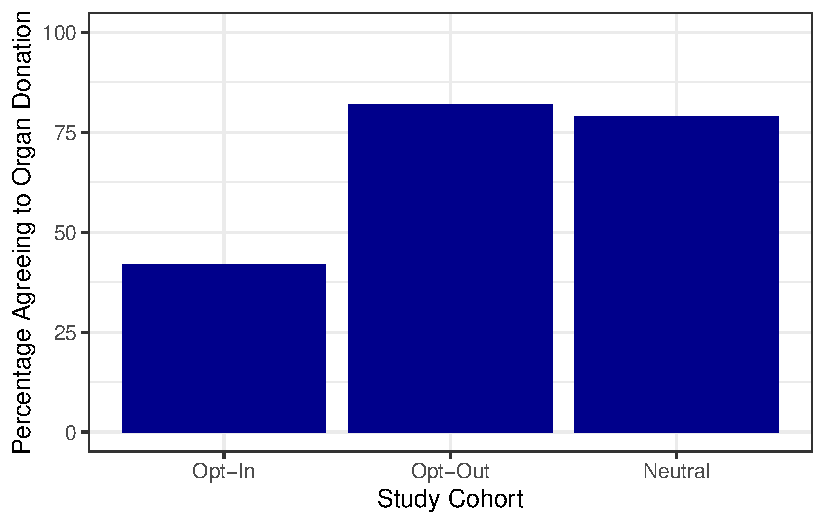
\includegraphics[width=0.8\textwidth,height=\textheight]{./images/fig-basics-organ-plot-1.pdf}

}

\caption{\label{fig-basics-organ-plot}Summary of the responses for the
Organ Donation Study described in
Example~\ref{exm-basics-organ-donation}.}

\end{figure}%

\section{Overview of Drawing
Inference}\label{overview-of-drawing-inference}

Let's begin by taking a step back and considering the big picture of how
data is turned into information. Every research question we pose, at its
heart, is trying to characterize a \textbf{population}, the group of
subjects of ultimate interest.

\begin{definition}[Population]\protect\hypertarget{def-population}{}\label{def-population}

The collection of subjects we would like to say something about.

\end{definition}

In the Organ Donation study (Example~\ref{exm-basics-organ-donation}),
the researchers would like to say something about Americans who are of
the age to consent to organ donation; in particular, they would like to
quantify how likely it is that someone from this group agrees to organ
donation. Therefore, the population is \emph{all Americans who are of
the age to consent to organ donation}.

In general, the subjects (or units of observation) in a population need
not be people; in some studies, the population could be a collection of
screws, cell phones, sheet metal\ldots whatever characterizes the
objects from which we would \emph{like to} obtain measurements. We use
the phrase ``like to'' because in reality it is often impossible (or
impractical) to observe the entire population. Instead, we make
observations on a subset of the population; this smaller group is known
as the \textbf{sample}.

\begin{definition}[Sample]\protect\hypertarget{def-sample}{}\label{def-sample}

The collection of subjects for which we actually obtain measurements
(data).

\end{definition}

\begin{tcolorbox}[enhanced jigsaw, breakable, titlerule=0mm, colframe=quarto-callout-note-color-frame, bottomtitle=1mm, opacityback=0, rightrule=.15mm, toptitle=1mm, arc=.35mm, bottomrule=.15mm, left=2mm, title=\textcolor{quarto-callout-note-color}{\faInfo}\hspace{0.5em}{Note}, leftrule=.75mm, coltitle=black, toprule=.15mm, colbacktitle=quarto-callout-note-color!10!white, colback=white, opacitybacktitle=0.6]

Some readers may associate ``subjects'' with people; to avoid this
confusion, you may prefer ``unit of observation'' to subject. In this
text, we use subject to mean any unit on which observations could be
taken.

\end{tcolorbox}

For each subject within the sample, we obtain a collection of
measurements forming our set of data. The goal of statistical modeling
is to use the sample (the group we actually observe) to say something
about the population of interest (the group we wish we had observed);
this process is known as \textbf{statistical inference} (illustrated in
Figure~\ref{fig-basics-statistical-process}).

\begin{definition}[Statistical
Inference]\protect\hypertarget{def-inference}{}\label{def-inference}

The process of using a sample to characterize some aspect of the
underlying population.

\end{definition}

\begin{figure}

\centering{

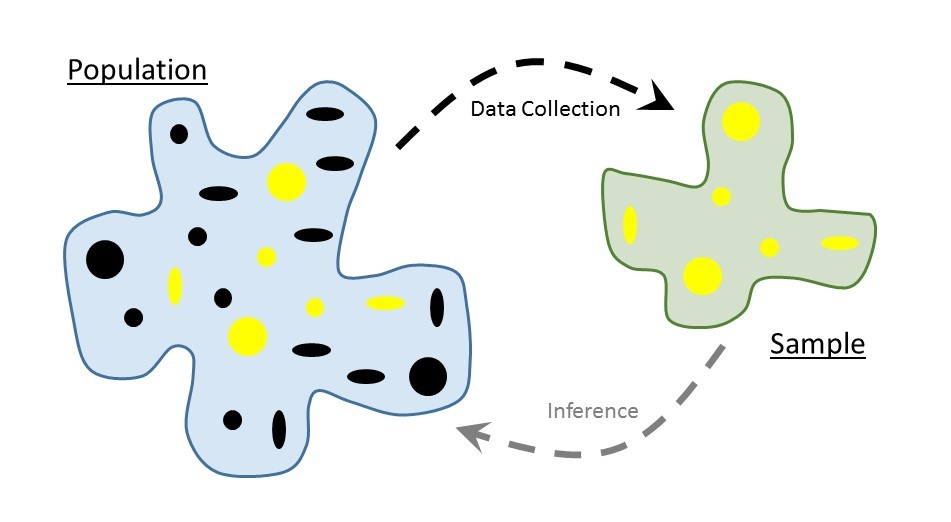
\includegraphics[width=0.8\textwidth,height=\textheight]{images/Basics-Stat-Process.jpg}

}

\caption{\label{fig-basics-statistical-process}Illustration of the
statistical process, using a sample to characterize some aspect of the
underlying population.}

\end{figure}%

\section{Anatomy of a Dataset}\label{anatomy-of-a-dataset}

Once we have our sample, we take measurements on each of the subjects
within this sample. These measurements form the data. When we hear the
word ``data,'' most of us envision a large spreadsheet. In reality, data
can take on many forms --- spreadsheets, images, text files,
unstructured text from a social media feed, etc. Regardless of the form,
all datasets contain information for each subject in the sample; this
information, the various measurements, are called \textbf{variables}.

\begin{definition}[Variable]\protect\hypertarget{def-variable}{}\label{def-variable}

A measurement, or category, describing some aspect of the subject.

\end{definition}

Variables come in one of two flavors. \textbf{Categorical} variables are
those which denote a grouping to which the subject belongs. Examples
include marital status, manufacturer, and experimental treatment group.
\textbf{Numeric} variables are those which take on values for which
ordinary arithmetic (e.g., addition and multiplication) makes sense.
Examples include height, age of a product, and diameter. Note that
sometimes numeric values are used to represent the levels of a
categorical variable in a dataset; for example, 0 may indicate ``No''
and 1 may indicate ``Yes'' for a variable capturing whether a person is
a registered organ donor. Therefore, just because a variable has a
numeric value does not make it a numeric variable; the key here is that
numeric variables are those for which arithmetic makes sense.

\begin{definition}[Categorical
Variable]\protect\hypertarget{def-categorical}{}\label{def-categorical}

Also called a ``qualitative variable,'' a measurement on a subject which
denotes a grouping or categorization.

\end{definition}

\begin{definition}[Numeric
Variable]\protect\hypertarget{def-numeric}{}\label{def-numeric}

Also called a ``quantitative variable,'' a measurement on a subject
which takes on a numeric value \emph{and} for which ordinary arithmetic
makes sense.

\end{definition}

While it may be natural to think of a dataset as a spreadsheet, not all
spreadsheets are created equal.

\begin{tcolorbox}[enhanced jigsaw, breakable, titlerule=0mm, colframe=quarto-callout-tip-color-frame, bottomtitle=1mm, opacityback=0, rightrule=.15mm, toptitle=1mm, arc=.35mm, bottomrule=.15mm, left=2mm, title=\textcolor{quarto-callout-tip-color}{\faLightbulb}\hspace{0.5em}{Characteristics of Well-Structured Data}, leftrule=.75mm, coltitle=black, toprule=.15mm, colbacktitle=quarto-callout-tip-color!10!white, colback=white, opacitybacktitle=0.6]

A well-structured dataset should adhere to the following
characteristics:

\begin{itemize}
\tightlist
\item
  Each column contains a unique variable.
\item
  Each record (row in the dataset) corresponds to a different
  observation of the variables.
\item
  If you have multiple datasets, they should include a column in the
  table that allows them to be linked (subject identifier).
\end{itemize}

\end{tcolorbox}

These characteristics ensure the data is properly formatted for an
analysis. Even unstructured data such as images or text files must be
processed prior to performing a statistical analysis.

\begin{tcolorbox}[enhanced jigsaw, breakable, titlerule=0mm, colframe=quarto-callout-warning-color-frame, bottomtitle=1mm, opacityback=0, rightrule=.15mm, toptitle=1mm, arc=.35mm, bottomrule=.15mm, left=2mm, title=\textcolor{quarto-callout-warning-color}{\faExclamationTriangle}\hspace{0.5em}{Warning}, leftrule=.75mm, coltitle=black, toprule=.15mm, colbacktitle=quarto-callout-warning-color!10!white, colback=white, opacitybacktitle=0.6]

We note the above description eliminates a common method of storing data
in engineering and scientific disciplines --- storing each sample in a
different column.

\end{tcolorbox}

To illustrate the above description, suppose we conduct a study
comparing the lifetime (in hours) of two brands of batteries. We measure
the lifetime of five batteries of Brand A and six of Brand B. It is
common to see a dataset like that in
Table~\ref{tbl-basics-poor-dataset}; the problem here is that the first
record of the dataset contains information on two different units of
observation. We have the lifetime from a battery of Brand A in the same
row as the lifetime from a battery of Brand B. This violates the second
characteristic of datasets described above.

\begin{table}

\caption{\label{tbl-basics-poor-dataset}Example of a common data
structure which does not correspond to the characteristics of
well-structured data we recommend. The data is from a hypothetical study
comparing battery lifetimes (hours).}

\centering{

\centering
\begin{tabular}[t]{cc}
\toprule
Brand A & Brand B\\
\midrule
\cellcolor{gray!10}{8.3} & \cellcolor{gray!10}{8.4}\\
5.1 & 8.6\\
\cellcolor{gray!10}{3.3} & \cellcolor{gray!10}{3.8}\\
5.3 & 4.1\\
\cellcolor{gray!10}{5.7} & \cellcolor{gray!10}{4.5}\\
\addlinespace
 & 4.0\\
\bottomrule
\end{tabular}

}

\end{table}%

In order to adhere to the characteristics of well-structured data
outlined above, we can reformat the data in
Table~\ref{tbl-basics-poor-dataset} to that shown in
Table~\ref{tbl-basics-good-dataset}. Here, each record represents a
unique observation and each column is a different variable. We have also
added a unique identifier.

\begin{table}

\caption{\label{tbl-basics-good-dataset}Example of a well-structured
dataset. The data is from a hypothetical study comparing battery
lifetimes (hours).}

\centering{

\centering
\begin{tabular}[t]{ccc}
\toprule
Battery & Brand & Lifetime\\
\midrule
\cellcolor{gray!10}{1} & \cellcolor{gray!10}{A} & \cellcolor{gray!10}{8.3}\\
2 & A & 5.1\\
\cellcolor{gray!10}{3} & \cellcolor{gray!10}{A} & \cellcolor{gray!10}{3.3}\\
4 & A & 5.3\\
\cellcolor{gray!10}{5} & \cellcolor{gray!10}{A} & \cellcolor{gray!10}{5.7}\\
\addlinespace
6 & B & 8.4\\
\cellcolor{gray!10}{7} & \cellcolor{gray!10}{B} & \cellcolor{gray!10}{8.6}\\
8 & B & 3.8\\
\cellcolor{gray!10}{9} & \cellcolor{gray!10}{B} & \cellcolor{gray!10}{4.1}\\
10 & B & 4.5\\
\addlinespace
\cellcolor{gray!10}{11} & \cellcolor{gray!10}{B} & \cellcolor{gray!10}{4.0}\\
\bottomrule
\end{tabular}

}

\end{table}%

It may take some time to get used to storing data in this format, but it
makes analysis easier and avoids time spent managing the data later.

\section{A Note on Codebooks}\label{a-note-on-codebooks}

A dataset on its own is meaningless if you cannot understand what the
values represent. \emph{Before} you access a dataset, you should always
review any available \textbf{codebooks}.

\begin{definition}[Codebook]\protect\hypertarget{def-codebook}{}\label{def-codebook}

Also called a ``data dictionary,'' these provide complete information
regarding the variables contained within a dataset.

\end{definition}

Some codebooks are excellent, with detailed descriptions of how the
variables were collected alongside appropriate units for the
measurements. Other codebooks give only an indication of what each
variable represents. Whenever you are working with previously collected
data, reviewing a codebook is the first step; and, you should be
prepared to revisit the codebook often throughout an analysis. When you
are collecting your own dataset, constructing a codebook is essential
for others to make use of your data.

\chapter{Case Study: Health Effects of the Deepwater Horizon Oil
Spill}\label{sec-caseDeepwater}

On the evening of April 20, 2010, the \emph{Deepwater Horizon}, an oil
drilling platform positioned off the coast of Louisiana, was engulfed in
flames as the result of an explosion. The drilling rig, leased and
operated by BP, had been tasked with drilling an oil well in water
nearly 5000 feet deep. Eleven personnel were killed in the explosion.
The following screenshot is from the initial coverage by the \emph{New
York Times}\footnote{\url{http://www.nytimes.com/2010/04/22/us/22rig.html?rref=collection\%2Ftimestopic\%2FOil\%20Spills&action=click&contentCollection=timestopics&region=stream&module=stream_unit&version=search&contentPlacement=1&pgtype=collection}}:

\begin{figure}

\centering{

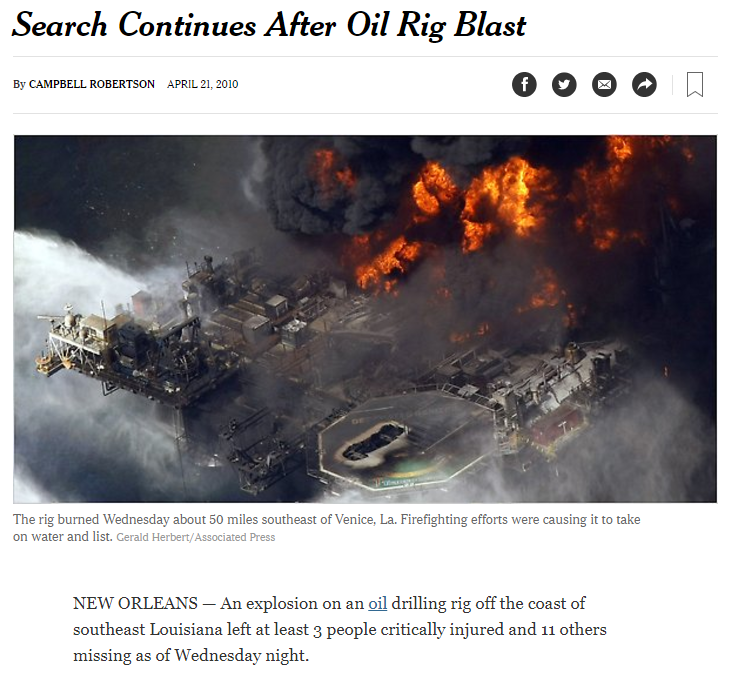
\includegraphics[width=0.8\textwidth,height=\textheight]{./images/Case-Deepwater-NYTclip.png}

}

\caption{\label{fig-casedeepwater-nytclip}\emph{New York Times} coverage
of the \emph{Deepwater Horizon} oil spill.}

\end{figure}%

The incident is considered the worst oil spill in US history, creating
an environmental disaster along the Gulf Coast. In addition to studying
the effects on the local environment, researchers have undertaken
studies to examine the short and long-term health effects caused by the
incident. As an example, we might ask whether volunteers who were
directly exposed to oil, such as when cleaning wildlife, are at higher
risk of respiratory irritation compared to those volunteers who were
helping with administrative tasks (and therefore were not directly
exposed to oil). An article appearing in \emph{The New England Journal
of Medicine} (Goldstein, Osofsky, and Lichtveld 2011) reported the
results from a health symptom survey performed in the Spring and Summer
of 2010 by the National Institute for Occupational Safety and Health. Of
54 volunteers assigned to wildlife cleaning and rehabilitation, 15
reported experiencing ``nose irritation, sinus problems, or sore
throat.'' Of 103 volunteers who had no exposure to oil, dispersants,
cleaners, or other chemicals, 16 reported experiencing ``nose
irritation, sinus problems, or sore throat.''

While a larger fraction of volunteers cleaning wildlife \emph{in the
study} reported respiratory symptoms compared to those who were not
directly exposed to irritants, would we expect similar results if we
were able to interview all volunteers? What about during a future oil
spill? Is there evidence that more than 1 in 5 volunteers who clean
wildlife will develop respiratory symptoms? What is a reasonable value
for the increased risk of respiratory symptoms for those volunteers with
direct exposure compared to those without?

In the first part of this text, we use this motivating example as the
context for discussing how research questions should be framed, methods
for data collection, summarizing and presenting data clearly,
quantifying the variability in an estimate, and quantifying the degree
to which the data disagrees with a proposed model. We capture these
ideas in what we call the \emph{Five Fundamental Ideas of Inference}. We
will also see that any statistical analysis moves between the components
of what we call the \emph{Distributional Quartet}. These two frameworks
allow us to describe the language and logic of inference, serving as a
foundation for the statistical thinking and reasoning needed to address
more complex questions encountered later in the text.

\chapter{Asking the Right Questions}\label{sec-questions}

The discipline of statistics is about turning data into information in
order to address some question. While there may be no such thing as a
stupid question, there are ill-posed questions --- those which cannot be
answered as stated. Consider the \href{01c-casedeepwater.qmd}{Deepwater
Horizon Case Study} (Chapter~\ref{sec-caseDeepwater}). It might seem
natural to ask ``if a volunteer cleans wildlife, will she develop
adverse respiratory symptoms?'' Let's consider the data. Of the 54
volunteers assigned to wildlife cleaning and rehabilitation, 15 reported
experiencing adverse respiratory symptoms (``nose irritation, sinus
problems, or sore throat''); while some volunteers developed symptoms,
others did not. It seems the answer to our question is then ``it
depends'' or ``maybe.'' This is an example of an \emph{ill-posed
question}. Such questions exist because of \textbf{variability}, the
fact that every subject in the population does not behave in exactly the
same way; that is, the value of a variable potentially differs from one
observation to the next. In our example not every volunteer had the same
reaction when directly exposed to oil.

It is variability that creates a need for the discipline of statistics;
in fact, you could think of statistics as the study and characterization
of variability. We must therefore learn to ask the \emph{right}
questions --- those which can be answered in the presence of
variability.

\begin{definition}[Variability]\protect\hypertarget{def-variability}{}\label{def-variability}

The notion that measurements differ from one observation to another.

\end{definition}

\begin{tcolorbox}[enhanced jigsaw, breakable, titlerule=0mm, colframe=quarto-callout-tip-color-frame, bottomtitle=1mm, opacityback=0, rightrule=.15mm, toptitle=1mm, arc=.35mm, bottomrule=.15mm, left=2mm, title=\textcolor{quarto-callout-tip-color}{\faLightbulb}\hspace{0.5em}{Big Idea}, leftrule=.75mm, coltitle=black, toprule=.15mm, colbacktitle=quarto-callout-tip-color!10!white, colback=white, opacitybacktitle=0.6]

The presence of variability makes some questions ill-posed; statistics
concerns itself with how to address questions in the presence of
variability.

\end{tcolorbox}

\section{Characterizing a Variable}\label{characterizing-a-variable}

Recall that the goal of statistical inference is to say something about
the population; as a result, any question we ask should then be about on
this larger group. The first step to constructing a well-posed question
is then to identify the population of interest for the study. For the
\href{01c-casedeepwater.qmd}{Deepwater Horizon Case Study}, it is
unlikely that we are only interested in these 54 observed volunteers
assigned to wildlife cleaning. In reality, we probably want to say
something about volunteers for any oil spill. The 54 volunteers in our
dataset form the sample, a subset from all volunteers who clean wildlife
following an oil spill. Our population of interest is comprised of all
volunteers who clean wildlife following an oil spill.

\begin{tcolorbox}[enhanced jigsaw, breakable, titlerule=0mm, colframe=quarto-callout-note-color-frame, bottomtitle=1mm, opacityback=0, rightrule=.15mm, toptitle=1mm, arc=.35mm, bottomrule=.15mm, left=2mm, title=\textcolor{quarto-callout-note-color}{\faInfo}\hspace{0.5em}{Note}, leftrule=.75mm, coltitle=black, toprule=.15mm, colbacktitle=quarto-callout-note-color!10!white, colback=white, opacitybacktitle=0.6]

When identifying the population of interest for a research question you
have, be specific! Suppose you are trying to estimate the average height
of trees. Are you really interested in \emph{all} trees? Or, are you
interested in Maple trees within the city limits of Terre Haute,
Indiana?

\end{tcolorbox}

Since we expect that the reaction to oil exposure --- the primary
variable of interest for this study, sometimes called the
\textbf{response} --- to vary from one individual to another, we cannot
ask a question about the \emph{value} of the reaction (whether they
experienced symptoms or not). Instead, we want to characterize the
\textbf{distribution} of the response.

\begin{definition}[Response]\protect\hypertarget{def-response}{}\label{def-response}

The primary variable of interest within a study. This is the variable
you would either like to explain or estimate.

\end{definition}

\begin{definition}[Distribution]\protect\hypertarget{def-distribution}{}\label{def-distribution}

The pattern of variability corresponding to a set of values.

\end{definition}

Notice that in this case, the response is a categorical variable;
describing the distribution of such a variable is equivalent to
describing how individuals are divided among the possible groups. With a
finite number of observations, we could present the number of
observations, the \textbf{frequency}, within each group. For example, of
the 54 volunteers, 15 experienced adverse symptoms and 39 did not. This
works well within the sample; however, as our population is infinitely
large (all volunteers cleaning wildlife following an oil spill),
reporting the frequencies is not appropriate. In this case, we report
the fraction of observations, the \textbf{relative frequency}, falling
within each group; this helps convey information about the distribution
of this variable. That is, the relative frequencies give us a sense of
which values of the variable are more or less common in the sample.

\begin{definition}[Frequency]\protect\hypertarget{def-frequency}{}\label{def-frequency}

The number of observations in a sample falling into a particular group
(level) defined by a categorical variable.

\end{definition}

\begin{definition}[Relative
Frequency]\protect\hypertarget{def-relative-frequency}{}\label{def-relative-frequency}

Also called the ``proportion,'' the fraction of observations falling
into a particular group (level) of a categorical variable.

\end{definition}

Numeric quantities, like the proportion, which summarize the
distribution of a variable within the population are known as
\textbf{parameters}.

\begin{definition}[Parameter]\protect\hypertarget{def-parameter}{}\label{def-parameter}

Numeric quantity which summarizes the distribution of a variable within
the \emph{population} of interest. Generally denoted by Greek letters in
statistical formulas.

\end{definition}

While the \emph{value} of a variable may vary across the population, the
\emph{parameter} is a single fixed constant which summarizes the
variable for that population. For example, the grade received on an exam
varies from one student to another in a class; but, the \emph{average
exam grade} is a fixed number which summarizes the class as a whole.
Well-posed questions can be constructed if we limit ourselves to
questions about the parameter. The second step in constructing
well-posed questions is then to identify the parameter of interest.

The questions we ask generally fall into one of two categories:

\begin{itemize}
\tightlist
\item
  Estimation: what \emph{proportion} of volunteers who clean wildlife
  following an oil spill will experience adverse respiratory symptoms?
\item
  Hypothesis Testing: is it reasonable no more than 1 in 5 volunteers
  who clean wildlife following an oil spill will experience adverse
  respiratory symptoms; or, is there evidence more than 1 in 5
  volunteers who clean wildlife following an oil spill will experience
  adverse respiratory symptoms?
\end{itemize}

\begin{definition}[Estimation]\protect\hypertarget{def-estimation}{}\label{def-estimation}

Using the sample to approximate the value of a parameter from the
underlying population.

\end{definition}

\begin{definition}[Hypothesis
Testing]\protect\hypertarget{def-hypothesis-testing}{}\label{def-hypothesis-testing}

Using a sample to determine if the data is consistent with a working
theory or if there is evidence to suggest the data is not consistent
with the theory.

\end{definition}

Since we do not get to observe the population (we only see the sample),
we cannot observe the value of the parameter. That is, we will never
know the true proportion of volunteers who experience symptoms. However,
we can determine what the data suggests about the population (that is
what inference is all about).

\begin{tcolorbox}[enhanced jigsaw, breakable, titlerule=0mm, colframe=quarto-callout-tip-color-frame, bottomtitle=1mm, opacityback=0, rightrule=.15mm, toptitle=1mm, arc=.35mm, bottomrule=.15mm, left=2mm, title=\textcolor{quarto-callout-tip-color}{\faLightbulb}\hspace{0.5em}{Big Idea}, leftrule=.75mm, coltitle=black, toprule=.15mm, colbacktitle=quarto-callout-tip-color!10!white, colback=white, opacitybacktitle=0.6]

Parameters are unknown values and can never, in general, be known.

\end{tcolorbox}

It turns out, the vast majority of research questions can be framed in
terms of a parameter. This is the first of what we consider the
\emph{Five Fundamental Ideas of Inference}.

\begin{tcolorbox}[enhanced jigsaw, breakable, titlerule=0mm, colframe=quarto-callout-important-color-frame, bottomtitle=1mm, opacityback=0, rightrule=.15mm, toptitle=1mm, arc=.35mm, bottomrule=.15mm, left=2mm, title=\textcolor{quarto-callout-important-color}{\faExclamation}\hspace{0.5em}{Fundamental Idea I}, leftrule=.75mm, coltitle=black, toprule=.15mm, colbacktitle=quarto-callout-important-color!10!white, colback=white, opacitybacktitle=0.6]

A research question can often be framed in terms of a parameter that
characterizes the population. Framing the question should then guide our
analysis.

\end{tcolorbox}

We now have a way of describing a well-posed question, a question which
can be addressed using data. Well posed questions are about the
population and can be framed in terms of a parameter which summarizes
that population. We now describe how these questions are typically
framed.

\section{Framing the Question}\label{framing-the-question}

In engineering and scientific applications, many questions fall under
the second category of \textbf{hypothesis testing}, which is a form of
model comparison in which data is collected to help the researcher
choose between two competing theories for the parameter of interest. In
this section, we consider the terminology surrounding specifying such
questions.

For the \href{01c-casedeepwater.qmd}{Deepwater Horizon Case Study}
suppose we are interested in addressing the following question:

\begin{quote}
Is there evidence that more than 1 in 5 volunteers who clean wildlife
following an oil spill will develop adverse respiratory symptoms?
\end{quote}

The question itself is about the population (all volunteers assigned to
clean wildlife following an oil spill) and is centered on a parameter
(the proportion who develop adverse respiratory symptoms). That is, this
is a well-posed question that can be answered with appropriate data. The
overall process for addressing these types of questions is similar to
conducting a trial in a court of law. In the United States, a trial has
the following essential steps:

\begin{enumerate}
\def\labelenumi{\arabic{enumi}.}
\tightlist
\item
  Assume the defendant is innocent.
\item
  Present evidence to establish guilt, to the contrary of innocence
  (prosecution's responsibility).
\item
  Consider the weight of the evidence presented (jury's responsibility).
\item
  Make a decision. If the evidence is ``beyond a reasonable doubt,'' the
  jury declares the defendant guilty; otherwise, the jury declares the
  defendant not guilty.
\end{enumerate}

The process of conducting a hypothesis test has similar essential steps:

\begin{enumerate}
\def\labelenumi{\arabic{enumi}.}
\tightlist
\item
  Assume the opposite of what we want the data to show (develop a
  working theory).
\item
  Gather data and compare it to the proposed model from step (1).
\item
  Quantify the likelihood of our data from step (2) under the proposed
  model.
\item
  If the likelihood is small, conclude the data is not consistent with
  the working model (there is evidence for what we want to show);
  otherwise, conclude the data is consistent with the working model
  (there is no evidence for what we want to show).
\end{enumerate}

Notice that a trial focuses not on proving guilt but on disproving
innocence; similarly, in statistics, we are able to establish evidence
\emph{against} a specified theory. This is one of several subtle points
in hypothesis testing. We will discuss these subtleties at various
points throughout the text and revisit the overall concepts often. Here,
we focus solely on that first step --- developing a working theory that
we want to \emph{disprove}.

\begin{tcolorbox}[enhanced jigsaw, breakable, titlerule=0mm, colframe=quarto-callout-note-color-frame, bottomtitle=1mm, opacityback=0, rightrule=.15mm, toptitle=1mm, arc=.35mm, bottomrule=.15mm, left=2mm, title=\textcolor{quarto-callout-note-color}{\faInfo}\hspace{0.5em}{Note}, leftrule=.75mm, coltitle=black, toprule=.15mm, colbacktitle=quarto-callout-note-color!10!white, colback=white, opacitybacktitle=0.6]

This process may seem counter-intuitive; it is natural to ask ``why
can't we prove guilt directly?'' However, when you disprove one
statement, you are proving that statement's opposite --- a technique
known in mathematics as ``proof by contradiction.'' So, our approach to
proving a statement is to disprove all other possibilities. It is
similar to the technique of the fictional detective Sherlock Holmes
(Doyle 1890, pg. 92): ``Eliminate all other factors, and the one which
remains must be the truth.''

\end{tcolorbox}

Consider the above question for the
\href{01c-casedeepwater.qmd}{Deepwater Horizon Case Study}. We want to
find evidence that the proportion experiencing adverse symptoms exceeds
0.20 (1 in 5). Therefore, we would like to \emph{disprove} (or provide
evidence \emph{against}) the statement that the proportion experiencing
adverse symptoms is no more than 0.20. This statement that we would like
to disprove is known as the \textbf{null hypothesis}; the opposite of
this statement, called the \textbf{alternative hypothesis}, captures
what we as the researchers would like to establish.

\begin{definition}[Null
Hypothesis]\protect\hypertarget{def-null-hypothesis}{}\label{def-null-hypothesis}

The statement (or theory) about the parameter that we would like to
\emph{disprove}. This is denoted \(H_0\), read ``H-naught'' or
``H-zero''.

\end{definition}

\begin{definition}[Alternative
Hypothesis]\protect\hypertarget{def-alternative-hypothesis}{}\label{def-alternative-hypothesis}

The statement (or theory) about the parameter capturing what we would
like to provide evidence \emph{for}; this is the opposite of the null
hypothesis. This is denoted \(H_1\) or \(H_a\), read ``H-one'' and
``H-A'' respectively.

\end{definition}

For the \href{01c-casedeepwater.qmd}{Deepwater Horizon Case Study}, we
write:

\begin{quote}
\(H_0:\) The proportion of volunteers assigned to clean wildlife
following an oil spill who experience adverse respiratory symptoms is no
more than 0.20.\\
\(H_1:\) The proportion of volunteers assigned to clean wildlife
following an oil spill who experience adverse respiratory symptoms
exceeds 0.20.
\end{quote}

Each hypothesis is a well-posed statement (about a parameter
characterizing the entire population), and the two statements are
exactly opposite of one another meaning only one can be a true
statement.

\begin{tcolorbox}[enhanced jigsaw, breakable, titlerule=0mm, colframe=quarto-callout-note-color-frame, bottomtitle=1mm, opacityback=0, rightrule=.15mm, toptitle=1mm, arc=.35mm, bottomrule=.15mm, left=2mm, title=\textcolor{quarto-callout-note-color}{\faInfo}\hspace{0.5em}{Note}, leftrule=.75mm, coltitle=black, toprule=.15mm, colbacktitle=quarto-callout-note-color!10!white, colback=white, opacitybacktitle=0.6]

When framing your questions, be sure your null hypothesis and
alternative hypothesis are exact opposites of one another, and ensure
the ``equality'' component \emph{always} goes in the null hypothesis.

\end{tcolorbox}

We can now collect data and determine if it is \emph{consistent} with
the null hypothesis (a statement similar to ``not guilty'') or if the
data provides \emph{evidence} against the null hypothesis and in favor
of the alternative (a statement similar to ``guilty'').

\begin{tcolorbox}[enhanced jigsaw, breakable, titlerule=0mm, colframe=quarto-callout-warning-color-frame, bottomtitle=1mm, opacityback=0, rightrule=.15mm, toptitle=1mm, arc=.35mm, bottomrule=.15mm, left=2mm, title=\textcolor{quarto-callout-warning-color}{\faExclamationTriangle}\hspace{0.5em}{Consistent vs.~Evidence}, leftrule=.75mm, coltitle=black, toprule=.15mm, colbacktitle=quarto-callout-warning-color!10!white, colback=white, opacitybacktitle=0.6]

The term ``consistent'' and ``reasonable'' will be used interchangeably
throughout the text; however, these terms differ substantially from the
term ``evidence.'' The data is said to be consistent with a statement if
the data is aligned with that statement. We have evidence for a
statement when the data is aligned with that statement \emph{and} it is
not aligned with the opposite of the statement (when we can disprove
something). We will see this develop more in Chapters
\ref{sec-samplingdistns} and \ref{sec-nulldistns}.

\end{tcolorbox}

Often these statements are written in a bit more of a mathematical
structure in which a Greek letter is used to represent the parameter of
interest. For example, we might write

\begin{quote}
Let \(\theta\) represent the proportion of volunteers (assigned to clean
wildlife following an oil spill) who experience adverse respiratory
symptoms.\\
\(H_0: \theta \leq 0.20\)\\
\(H_1: \theta > 0.20\)
\end{quote}

In the above statements, \(\theta\) represents the parameter of
interest; the value 0.20 is known as the \textbf{null value}.

\begin{definition}[Null
Value]\protect\hypertarget{def-null-value}{}\label{def-null-value}

The value associated with the equality component of the null hypothesis;
it forms the threshold or boundary between the hypotheses. Note: not all
questions of interest require a null value be specified.

\end{definition}

\begin{tcolorbox}[enhanced jigsaw, breakable, titlerule=0mm, colframe=quarto-callout-tip-color-frame, bottomtitle=1mm, opacityback=0, rightrule=.15mm, toptitle=1mm, arc=.35mm, bottomrule=.15mm, left=2mm, title=\textcolor{quarto-callout-tip-color}{\faLightbulb}\hspace{0.5em}{Big Idea}, leftrule=.75mm, coltitle=black, toprule=.15mm, colbacktitle=quarto-callout-tip-color!10!white, colback=white, opacitybacktitle=0.6]

Hypothesis testing is a form of statistical inference in which we
quantify the evidence \emph{against} a working theory (captured by the
null hypothesis). We essentially argue that the data supports the
alternative if it is not consistent with the working theory.

\end{tcolorbox}

This section has focused on developing the null and alternative
hypothesis when our question of interest is best characterized as one of
comparing models or evaluating a particular statement. If our goal is
estimation, a null and alternative hypothesis are not applicable. For
example, we might have the following goal:

\begin{quote}
Estimate the proportion of volunteers (assigned to clean wildlife
following an oil spill) who experience adverse respiratory symptoms.
\end{quote}

In this version of our research ``question'' there is no statement which
needs to be evaluated. We are interested in estimation, not hypothesis
testing and thus there is no corresponding null and alternative
hypothesis.

\begin{tcolorbox}[enhanced jigsaw, breakable, titlerule=0mm, colframe=quarto-callout-note-color-frame, bottomtitle=1mm, opacityback=0, rightrule=.15mm, toptitle=1mm, arc=.35mm, bottomrule=.15mm, left=2mm, title=\textcolor{quarto-callout-note-color}{\faInfo}\hspace{0.5em}{Process for Framing a Question}, leftrule=.75mm, coltitle=black, toprule=.15mm, colbacktitle=quarto-callout-note-color!10!white, colback=white, opacitybacktitle=0.6]

In order to frame a research question, consider the following steps:

\begin{enumerate}
\def\labelenumi{\arabic{enumi}.}
\tightlist
\item
  Identify the population of interest.\\
\item
  Identify the parameter(s) of interest.
\item
  Determine if you are interested in estimating the parameter(s) or
  quantifying the evidence against some working theory.\\
\item
  If you are interested in testing a working theory, make the null
  hypothesis the working theory and the alternative hypothesis the exact
  opposite statement (capturing what you want to provide evidence for).
\end{enumerate}

\end{tcolorbox}

\chapter{Gathering the Evidence (Data Collection)}\label{sec-data}

Consider again the goal of statistical inference --- to use a sample as
a snapshot to say something about the underlying population (see
Figure~\ref{fig-data-statistical-process}). This generally provokes
unease in people, leading to a distrust of statistical results. In this
section we attack that distrust head on.

\begin{figure}

\centering{

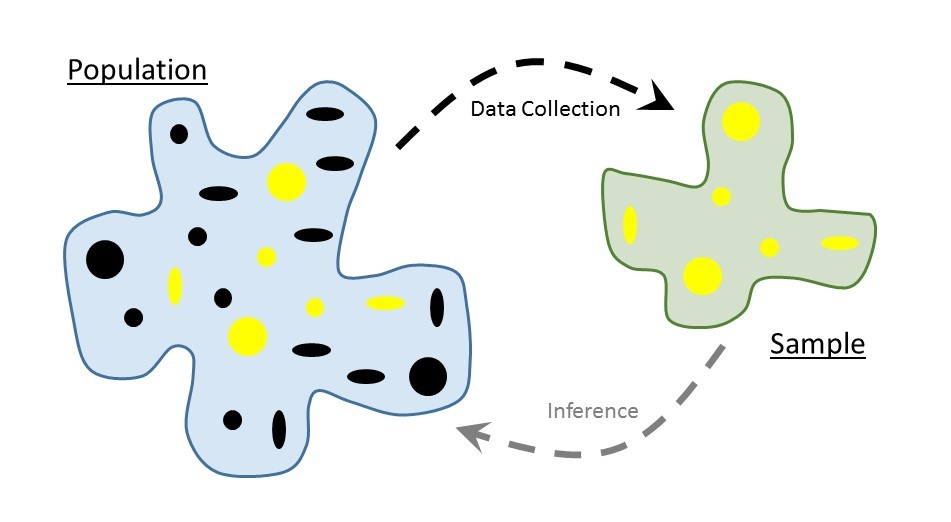
\includegraphics[width=0.8\textwidth,height=\textheight]{images/Basics-Stat-Process.jpg}

}

\caption{\label{fig-data-statistical-process}Illustration of the
statistical process (reprint of
Figure~\ref{fig-basics-statistical-process}).}

\end{figure}%

\section{What Makes a Sample
Reliable}\label{what-makes-a-sample-reliable}

If we are going to have some amount of faith in the statistical results
we produce, we must have data in which we can place our trust. \emph{The
Treachery of Images} (Figure~\ref{fig-data-pipe-img}) is a canvas
painting depicting a pipe, below which the artist wrote the French
phrase ``This is not a pipe.'' Regarding the painting, the artist said

\begin{quote}
The famous pipe. How people reproached me for it! And yet, could you
stuff my pipe? No, it's just a representation, is it not? So if I had
written on my picture ``This is a pipe,'' I'd have been lying!
\end{quote}

\begin{figure}

\centering{

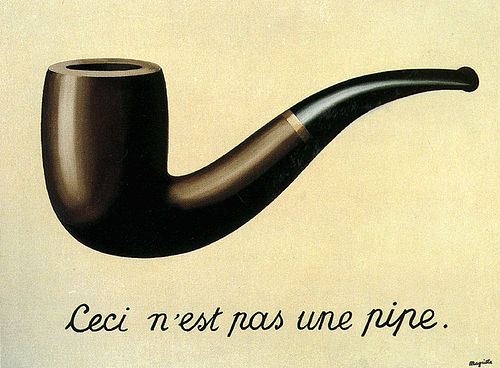
\includegraphics[width=0.8\textwidth,height=\textheight]{./images/Data-Pipe.jpg}

}

\caption{\label{fig-data-pipe-img}\emph{The Treachery of Images} by René
Magritte.}

\end{figure}%

Just as a painting is a representation of the object it depicts, so a
sample should be a representation of the population under study. This is
the primary requirement if we are to rely on the resulting data.

\begin{tcolorbox}[enhanced jigsaw, breakable, titlerule=0mm, colframe=quarto-callout-tip-color-frame, bottomtitle=1mm, opacityback=0, rightrule=.15mm, toptitle=1mm, arc=.35mm, bottomrule=.15mm, left=2mm, title=\textcolor{quarto-callout-tip-color}{\faLightbulb}\hspace{0.5em}{Big Idea}, leftrule=.75mm, coltitle=black, toprule=.15mm, colbacktitle=quarto-callout-tip-color!10!white, colback=white, opacitybacktitle=0.6]

In order for a statistical analysis to be reliable, the sample must be
\emph{representative} of the population under study.

\end{tcolorbox}

We need to be careful to not get carried away in our expectations. What
constitutes ``representative'' really depends on the question, just as
an artist chooses their depiction based on how they want to represent
the object. Let's consider the following example.

\begin{example}[School
Debt]\protect\hypertarget{exm-data-school-debt}{}\label{exm-data-school-debt}

In addition to a degree, college graduates also tend to leave with a
large amount of debt due to college loans. In 2012, a graduate with a
student loan had an average debt of \$29,400; for graduates from private
non-profit institutions, the average debt was \$32,300\footnote{http://ticas.org/sites/default/files/pub\_files/Debt\_Facts\_and\_Sources.pdf}.

Suppose we are interested in determining the average amount of debt in
student loans carried by a graduating senior from Rose-Hulman Institute
of Technology, a small private non-profit engineering school. There are
many faculty at Rose-Hulman who choose to send their children to the
institute. Suppose we were to ask 25 such faculty members who have a
child that attended the institute to report the amount of student loans
their children carried upon graduation from Rose-Hulman. Further,
suppose we compile the responses and compute the average amount of debt.
Using the data, we might report that based on our study, there is
significant evidence the average debt carried by a graduate of
Rose-Hulman is far below the \$32,300 reported above (great news for
this year's graduating class)!

Why should we be hesitant to trust the results from our study?

\end{example}

Many objections to statistical results stem from a distrust of whether
the data (the sample) is really representative of the population of
interest. Rose-Hulman, like many other universities, has a policy that
the children of faculty may attend their university (assuming
admittance) tuition-free. We would therefore expect their children to
carry much less debt than the typical graduating senior. There is a
mismatch between the group we would like to study and the data we have
collected.

This example provides a nice backdrop for discussing what it means to be
representative. First, let's define our population; in this case, we are
interested in graduating seniors from Rose-Hulman. The variable of
interest is the amount of debt carried in student loans; the parameter
of interest is then the \emph{average} amount of debt in student loans
carried by graduating seniors of Rose-Hulman. However, the sample
consists of only graduating seniors of Rose-Hulman \emph{who have a
parent employed by the institute}.

With regard to grade point average, the students in our sample are
probably similar to all graduating seniors; the starting salary of the
students in our sample is probably similar to all graduating seniors;
the fraction of mechanical engineering majors versus math majors is
probably similar. So, in many regards the sample is representative of
the population; however, it fails to be representative with regard to
the variable of interest. This is our concern. The amount of debt
carried by students in our sample is not representative of that debt
carried by all graduating seniors from the university.

\begin{tcolorbox}[enhanced jigsaw, breakable, titlerule=0mm, colframe=quarto-callout-note-color-frame, bottomtitle=1mm, opacityback=0, rightrule=.15mm, toptitle=1mm, arc=.35mm, bottomrule=.15mm, left=2mm, title=\textcolor{quarto-callout-note-color}{\faInfo}\hspace{0.5em}{Note}, leftrule=.75mm, coltitle=black, toprule=.15mm, colbacktitle=quarto-callout-note-color!10!white, colback=white, opacitybacktitle=0.6]

When thinking about whether a sample is representative, focus your
attention to the characteristics specific to your research question or
with regard to how you intend to generalize the results.

\end{tcolorbox}

Does that mean the sample we collected in
Example~\ref{exm-data-school-debt} is useless? Yes and no. The sample
collected cannot be used to answer our initial question of interest
since it is not representative of our population. No statistical method
can fix bad data; statistics adheres to the ``garbage-in, garbage-out''
phenomena. If the data is bad, no analysis will undo that. However,
while the sample cannot be used to answer our initial question, it could
be used to address a different question:

\begin{quote}
What is the average amount of debt in student loans carried by
graduating seniors from Rose-Hulman whose parent is a faculty member at
the institute?
\end{quote}

For this revised question, the sample may indeed be representative. If
we are working with previously collected data, we must consider the
population to which our results will generalize. That is, for what
population is the given sample representative? If we are collecting our
data, we need to be sure we collect data in such a way that the data is
representative of our target population. Let's first look at what
\emph{not} to do.

\section{Poor Methods of Data
Collection}\label{poor-methods-of-data-collection}

Example~\ref{exm-data-school-debt} is an example of a ``convenience
sample,'' when the subjects in the sample are chosen simply due to ease
of collection. Examples include surveying students only in your sorority
when you are interested in all students who are part of a sorority on
campus; taking soil samples from only your city when you are interested
in the soil for the entire state; and, obtaining measurements from only
one brand of phone, because it was the only one you could afford on your
budget, when you are interested in studying all cell phones on the
market. A convenience sample is unlikely to be representative if there
is a relationship between the ease of collection and the variable under
study. This was true in the School Debt example; the relationship of a
student to a faculty member, which is what increased the ease of
collection, was directly related to the amount of debt they carried. As
a result, the resulting sample was not representative of the population.

When conducting a survey with human subjects, it is common to only
illicit responses from volunteers. Such ``volunteer samples'' tend to
draw in those with extreme opinions. Consider product ratings on Amazon.
Individual ratings tend to cluster around 5's and 1's. This is because
those customers who take time to submit a review (which is voluntary)
tend to be those who are really thrilled with their product (and want to
encourage others to purchase it) and those who are really disappointed
with their purchase (and want to encourage others to avoid it). Such
surveys often fail to capture those individuals in the population who
have ``middle of the road'' opinions.

We could not possibly name all the poor methods for collecting a sample;
but, poor methods all share something in common --- it is much more
likely the resulting sample is not representative. Failing to be
representative results in \textbf{biased} estimates of the parameter.

\begin{definition}[Bias]\protect\hypertarget{def-bias}{}\label{def-bias}

A set of measurements is said to be biased if they are
\emph{consistently} too high (or too low). Similarly, an estimate of a
parameter is said to be biased if it is \emph{consistently} too high (or
too low).

\end{definition}

To illustrate the concept of bias, consider shooting at a target as in
Figure~\ref{fig-data-bias}. We can consider the center of our target to
be the parameter we would like to estimate within the population; in
this case, some measure of center. The values in our sample (the strikes
on the target) will vary around the parameter; while we do not expect
any one value to hit the target precisely, a ``representative'' sample
is one in which the values tend to be clustered about the parameter
(unbiased). When the sample is not representative, the values in the
sample tend to cluster off the mark (biased). Notice that to be
unbiased, it may be that not a single value in the sample is perfect,
but aggregated together, they point in the right direction. So, bias is
not about an individual measurement being an ``outlier,'' (more on those
in Chapter~\ref{sec-summaries}) but about \emph{consistently} shooting
in the wrong direction.

\begin{figure}

\centering{

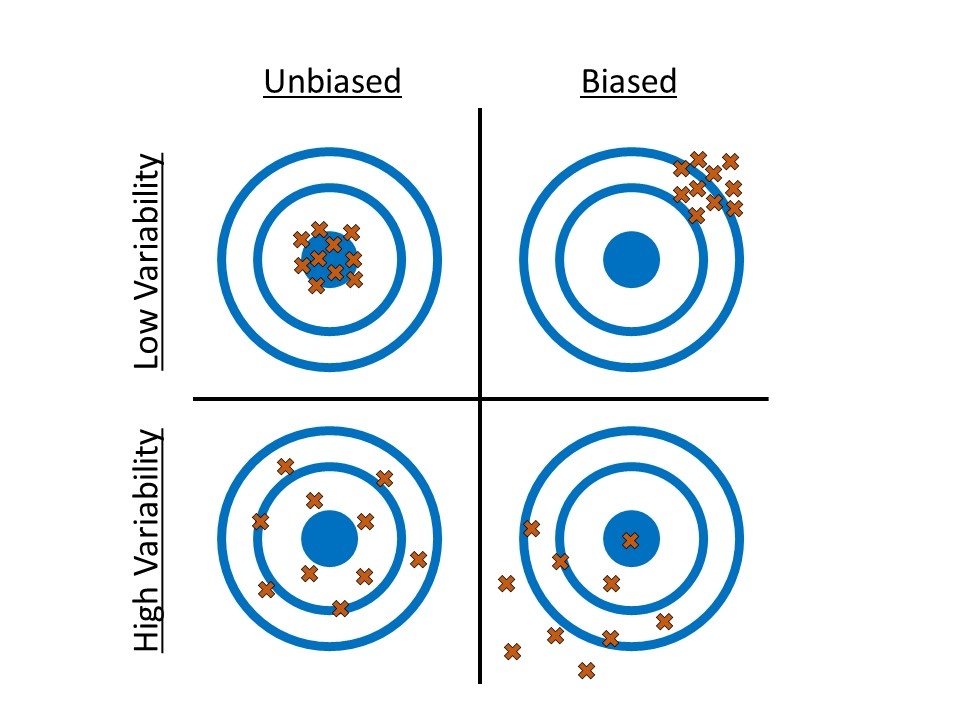
\includegraphics[width=0.8\textwidth,height=\textheight]{./images/Data-Bias.jpg}

}

\caption{\label{fig-data-bias}Illustration of bias and precision.}

\end{figure}%

\begin{tcolorbox}[enhanced jigsaw, breakable, titlerule=0mm, colframe=quarto-callout-warning-color-frame, bottomtitle=1mm, opacityback=0, rightrule=.15mm, toptitle=1mm, arc=.35mm, bottomrule=.15mm, left=2mm, title=\textcolor{quarto-callout-warning-color}{\faExclamationTriangle}\hspace{0.5em}{Accuracy vs.~Precision}, leftrule=.75mm, coltitle=black, toprule=.15mm, colbacktitle=quarto-callout-warning-color!10!white, colback=white, opacitybacktitle=0.6]

There is a difference between \emph{accuracy} and \emph{precision}.
Generally, \emph{accuracy} refers to location (and therefore relates to
bias); we say a process is accurate when it is unbiased.
\emph{Precision} refers to the variability; data which is more precise
has less variability.

\end{tcolorbox}

\begin{tcolorbox}[enhanced jigsaw, breakable, titlerule=0mm, colframe=quarto-callout-tip-color-frame, bottomtitle=1mm, opacityback=0, rightrule=.15mm, toptitle=1mm, arc=.35mm, bottomrule=.15mm, left=2mm, title=\textcolor{quarto-callout-tip-color}{\faLightbulb}\hspace{0.5em}{Big Idea}, leftrule=.75mm, coltitle=black, toprule=.15mm, colbacktitle=quarto-callout-tip-color!10!white, colback=white, opacitybacktitle=0.6]

Biased results are typically due to poor sampling methods that result in
a sample which is not representative of the population of interest.

\end{tcolorbox}

The catch (there is always a catch) is that we will never \emph{know}
with certainty if a sample is actually representative or not. In
practice, we critically examine the method in which the sample was
collected, and we use summaries of the sample to make educated decisions
on whether to generalize the results. Better, however, is to employ
methods of data collection that help to minimize the bias in the sample.

\section{Preferred Methods of
Sampling}\label{preferred-methods-of-sampling}

No method guarantees a perfectly representative sample; but, we can take
measures to reduce or eliminate bias. A useful strategy is to employ
\emph{randomization}. This is summarized in our second Fundamental Idea.

\begin{tcolorbox}[enhanced jigsaw, breakable, titlerule=0mm, colframe=quarto-callout-important-color-frame, bottomtitle=1mm, opacityback=0, rightrule=.15mm, toptitle=1mm, arc=.35mm, bottomrule=.15mm, left=2mm, title=\textcolor{quarto-callout-important-color}{\faExclamation}\hspace{0.5em}{Fundamental Idea II}, leftrule=.75mm, coltitle=black, toprule=.15mm, colbacktitle=quarto-callout-important-color!10!white, colback=white, opacitybacktitle=0.6]

If data is to be useful for making conclusions about the population, a
process referred to as drawing inference, proper data collection is
crucial. Randomization can play an important role ensuring a sample is
representative and that inferential conclusions are appropriate.

\end{tcolorbox}

Consider the School Debt example (Example~\ref{exm-data-school-debt})
again. Suppose instead of the data collection strategy described there,
we had done the following:

\begin{quote}
We constructed a list of all graduating seniors from the institute. We
placed the name of each student on an index card; then, we thoroughly
shuffled the cards and chose the top 25 cards. For these 25 individuals,
we recorded the amount of debt in student loans each carried.
\end{quote}

This essentially describes using a lottery to select the sample. This
popular method is known as taking a \textbf{simple random sample}. By
conducting a lottery, we make it very unlikely that our sample consists
of only students with a very small amount of student debt (as occurred
when we used a convenience sample).

\begin{definition}[Simple Random
Sample]\protect\hypertarget{def-simple-random-sample}{}\label{def-simple-random-sample}

Often abbreviated SRS, this is a sample of size \(n\) such that
\emph{every} collection of size \(n\) is equally likely to be the
resulting sample. This is equivalent to a lottery.

\end{definition}

\begin{tcolorbox}[enhanced jigsaw, breakable, titlerule=0mm, colframe=quarto-callout-note-color-frame, bottomtitle=1mm, opacityback=0, rightrule=.15mm, toptitle=1mm, arc=.35mm, bottomrule=.15mm, left=2mm, title=\textcolor{quarto-callout-note-color}{\faInfo}\hspace{0.5em}{Note}, leftrule=.75mm, coltitle=black, toprule=.15mm, colbacktitle=quarto-callout-note-color!10!white, colback=white, opacitybacktitle=0.6]

It is convention to use \(n\) to represent the sample size.

\end{tcolorbox}

The primary benefit of a simple random sample is that it removes bias.
More specifically, the \emph{process} of simple random sampling is
unbiased; that is, this process does \emph{not} produce values which are
\emph{consistently} too high or low.

There are situations in which a simple random sample does not suffice.
Again, consider our School Debt example. The Rose-Hulman student body is
predominantly domestic, with only about 3\% of the student body being
international students. But, suppose we are interested in comparing the
average debt carried between international and domestic students. It is
very likely, by chance alone, that in a simple random sample of 25
students none will be international. Instead of a simple random sample,
we might consider taking a sample of 13 domestic students and a sample
of 12 international students; this is an example of a \textbf{stratified
random sample}. This approach is useful when there is a natural grouping
of interest within the population.

\begin{definition}[Stratified Random
Sample]\protect\hypertarget{def-stratified-random-sample}{}\label{def-stratified-random-sample}

A sample in which the population is first divided into groups, or
strata, based on a characteristic of interest; a simple random sample is
then taken within each group.

\end{definition}

\begin{tcolorbox}[enhanced jigsaw, breakable, titlerule=0mm, colframe=quarto-callout-warning-color-frame, bottomtitle=1mm, opacityback=0, rightrule=.15mm, toptitle=1mm, arc=.35mm, bottomrule=.15mm, left=2mm, title=\textcolor{quarto-callout-warning-color}{\faExclamationTriangle}\hspace{0.5em}{Warning}, leftrule=.75mm, coltitle=black, toprule=.15mm, colbacktitle=quarto-callout-warning-color!10!white, colback=white, opacitybacktitle=0.6]

Note that a stratified random sample essentially results in a
representative sample \emph{within} each strata. However, the combined
sample may not be representative of the population. If there is interest
in using the sample in its entirety, instead of comparing the strata in
some way, advanced statistical methodology is required. See texts on
analyzing ``complex survey design'' for a more thorough discussion. Our
text will not consider such cases.

\end{tcolorbox}

There are countless sampling techniques used in practice. The two
described above can be very useful starting points for developing a
custom method suitable for a particular application. Their benefit stems
from their use of randomization as it limits researcher influence on the
composition of the sample and therefore minimizes bias.

This section is entitled ``Preferred Methods'' because while these
methods are ideal, they are not always practical. Consider the Deepwater
Horizon Case Study described in Chapter~\ref{sec-caseDeepwater};
conceptually, we can take a simple random sample of the volunteers for
our study. However, as with any study involving human subjects,
researchers would be required to obtain consent from each subject in the
study. That is, any individual has the right to refuse to participate in
the study. Therefore, it is unlikely that a simple random sample as
described above could be obtained. While random selection is a nice
tool, the goal is a sample which is \emph{representative} of the
population. While random sampling is helpful for accomplishing this, we
may need to appeal to the composition of the sample itself to justify
its use. \emph{Based on the characteristics of those willing to
participate in the study, do we feel the study participants form a
representative group of all volunteers?} That is the essential question.
This is often why studies report a table summarizing participant
demographics such as age, gender, etc. It is also why it is extremely
important for researchers to describe how observations were obtained so
that readers may make the judgement for themselves whether the sample is
representative.

\section{Two Types of Studies}\label{two-types-of-studies}

Thinking about how the data was collected helps us determine how the
results generalize beyond the sample itself (to what population the
results apply). When our question of interest is about the relationship
between two variables (as most questions are), we must also carefully
consider the study design. Too often separated from the statistical
analysis that follows, keeping the study design in mind should guide the
analysis as well as inform us about the conclusions we can draw. While
we will discuss study design more fully in Chapter~\ref{sec-anovadata},
we introduce some of the concepts here.

In order to illustrate how study design can impact the results, consider
the following example.

\begin{example}[Kangaroo
Care]\protect\hypertarget{exm-data-kangaroo}{}\label{exm-data-kangaroo}

At birth, infants have low levels of Vitamin K, a vitamin needed in
order to form blood clots. Though rare, without the ability for her
blood to clot, an infant could develop a serious bleed. In order to
prevent this, the American Academy of Pediatrics recommends that all
infants be given a Vitamin K shot shortly after birth in order to raise
Vitamin K levels. As with any shot, there is typically discomfort to the
infant, which can be very discomforting to new parents.

Kangaroo Care is a method of holding a baby which emphasizes
skin-to-skin contact. The child, who is dressed only in a diaper, is
placed upright on the parent's bare chest; a light blanket is draped
over the child. Suppose we are interested in determining if utilizing
the method while giving the child a Vitamin K shot reduces the
discomfort in the infant, as measured by the total amount of time the
child cries following the shot.

Within this context, contrast the following two potential study designs:

\begin{enumerate}
\def\labelenumi{(\Alph{enumi})}
\tightlist
\item
  We allow the attending nurse to determine whether Kangaroo Care is
  initiated prior to giving the Vitamin K shot. Following the shot, we
  record the total time (in seconds) the child cries.\\
\item
  We flip a coin. If it comes up heads, the nurse should have the
  parents implement Kangaroo Care prior to giving the Vitamin K shot; if
  it comes up tails, the nurse should give the Vitamin K shot without
  implementing Kangaroo Care. Following the shot, we record the total
  time (in seconds) the child cries.
\end{enumerate}

Note, in both study designs (A) and (B), we only consider term births
which have no complications to avoid situations that might alter the
timing of the Vitamin K shot or the ability to implement Kangaroo Care.

\end{example}

Note that there are some similarities in the two study designs:

\begin{itemize}
\tightlist
\item
  The underlying population is the same for both designs: infants born
  at term with no complications.
\item
  There are two groups being compared in both designs: the ``Kangaroo
  Care'' group and the ``no Kangaroo Care'' group.
\item
  The response (variable of interest) is the same in both designs: the
  time (in seconds) the infant cries.
\item
  There is action taken by the researcher in both designs: a Vitamin K
  shot is given to the child.
\end{itemize}

There is one prominent difference between the two study designs:

\begin{itemize}
\tightlist
\item
  For design (A), the choice of Kangaroo Care is left up to the nurse
  (self-selected); for design (B), the choice of Kangaroo is
  \emph{assigned} to the nurse by the researcher, and this selection is
  made \emph{at random}.
\end{itemize}

Design (A) is an example of an \textbf{observational study}; design (B)
is a an example of a \textbf{controlled experiment}.

\begin{definition}[Observational
Study]\protect\hypertarget{def-observational-study}{}\label{def-observational-study}

A study in which each subject ``self-selects'' into one of groups being
compared in the study. The phrase ``self-selects'' is used very loosely
here and can include studies for which the groups are defined by an
inherent characteristic or are chosen haphazardly.

\end{definition}

\begin{definition}[Controlled
Experiment]\protect\hypertarget{def-controlled-experiment}{}\label{def-controlled-experiment}

A study in which each subject is \emph{randomly} assigned to one of the
groups being compared in the study.

\end{definition}

It is common to think that anytime the environment is ``controlled'' by
the researcher that a controlled experiment is taking place, but the
defining characteristic is the random assignment to groups (sometimes
referred to as the \emph{factor} under study or \emph{treatment}
groups). In the example above, both study designs involved a controlled
setting (the delivery room of a hospital) in which trained staff (the
nurse) deliver the shot. However, only design (B) is a controlled
experiment because the researchers randomly determined which treatment
the infant would receive.

To understand the impact of random allocation, suppose that we had
conducted a study using design (A); further, the results of the study
suggest that those infants who were given a shot while using Kangaroo
Care cried for a shorter time period, on average. Can we conclude that
it was the Kangaroo Care that led to the shorter crying time? Maybe.
Consider the following two potential explanations for the resulting
data:

\begin{enumerate}
\def\labelenumi{(\arabic{enumi})}
\tightlist
\item
  Kangaroo Care is very effective; as a result, those children who are
  given Kangaroo Care cry for less time, on average, following the
  Vitamin K shot.\\
\item
  It turns out that those nurses who choose to implement Kangaroo Care
  (remember, they have a choice under design (A) whether they implement
  the method) are also the nurses with a gentler bedside manner.
  Therefore, these nurses tend to be very gentle when giving the Vitamin
  K shot whereas the nurses who choose not to implement Kangaroo Care
  tend to jab the needle when giving the shot. The reduced crying time
  is not a result of the Kangaroo Care but the manner in which the shot
  was given.
\end{enumerate}

The problem is that we are unable to determine which of the explanations
is correct under study design (A). Given the data we have collected, we
are unable to tease out the effect of the Kangaroo Care from that of the
nurse's bedside manner. As a result, we are able to say we observed an
\emph{association} between the use of Kangaroo Care and reduced crying
time, but we are unable to conclude that Kangaroo Care \emph{caused} a
reduction in the crying time (that is, the reduced crying time may be
due to something else, like the bedside manner of the nurse). In this
hypothetical scenario, the nurse's bedside manner is called a
\textbf{confounder}.

\begin{definition}[Confounding]\protect\hypertarget{def-confounding}{}\label{def-confounding}

When the effect of a variable on the response is mis-represented due to
the presence of a third, potentially unobserved, variable known as a
confounder.

\end{definition}

\begin{tcolorbox}[enhanced jigsaw, breakable, titlerule=0mm, colframe=quarto-callout-note-color-frame, bottomtitle=1mm, opacityback=0, rightrule=.15mm, toptitle=1mm, arc=.35mm, bottomrule=.15mm, left=2mm, title=\textcolor{quarto-callout-note-color}{\faInfo}\hspace{0.5em}{Note}, leftrule=.75mm, coltitle=black, toprule=.15mm, colbacktitle=quarto-callout-note-color!10!white, colback=white, opacitybacktitle=0.6]

While both result in estimates we may not trust, confounding is not
equivalent to a biased sample.

\end{tcolorbox}

Confounders can mask the relationship between the factor under study and
the response. Did you know there is a documented association between ice
cream sales and the risk of shark attacks? As ice cream sales increase,
the risk of a shark attack also tends to increase. This does not mean
that if a small city in the Midwest increases its ice cream sales that
the citizens are at higher risk of being attacked by a shark. As
Figure~\ref{fig-data-confounding} illustrates, there is a confounder ---
temperature. As the temperatures increase, people tend to buy more ice
cream; as the temperature increases, people tend to go to the beach,
thereby increasing the risk of a shark attack. The two variables, ice
cream sales and shark attacks, appear to be related as a result of the
confounder of temperature.

\begin{figure}

\centering{

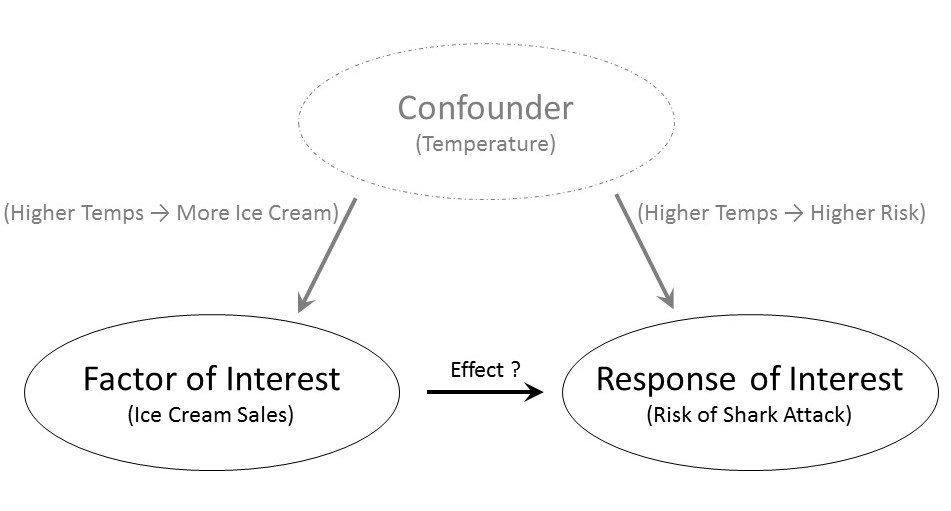
\includegraphics[width=0.8\textwidth,height=\textheight]{./images/Data-Confounding.jpg}

}

\caption{\label{fig-data-confounding}Illustration of a confounding
variable. The confounder, related to both the response and the factor of
interest (or treatment) can make it appear as though there is a causal
relationship when none exists.}

\end{figure}%

\begin{tcolorbox}[enhanced jigsaw, breakable, titlerule=0mm, colframe=quarto-callout-tip-color-frame, bottomtitle=1mm, opacityback=0, rightrule=.15mm, toptitle=1mm, arc=.35mm, bottomrule=.15mm, left=2mm, title=\textcolor{quarto-callout-tip-color}{\faLightbulb}\hspace{0.5em}{Big Idea}, leftrule=.75mm, coltitle=black, toprule=.15mm, colbacktitle=quarto-callout-tip-color!10!white, colback=white, opacitybacktitle=0.6]

Confounders are variables that influence \emph{both} the factor of
interest and the response.

\end{tcolorbox}

Observational studies are subject to confounding; thus, controlled
experiments are often considered the gold standard in research because
they allow us to infer cause-and-effect relationships from the data.
Controlled experiments allow for causal interpretations because the
random allocation to the levels of the factor removes the impact of
confounders. Let's return to the hypothetical Vitamin-K study in
Example~\ref{exm-data-kangaroo}. Suppose there are nurses with a gentle
bedside manner and those who are a little less gentle. If we randomly
determine which infants receive Kangaroo Care, then for every gentle
nurse who is told to implement Kangaroo Care while giving the shot,
there tends to be a gentle nurse who is told to not implement Kangaroo
Care. Similarly, for every less-gentle nurse who is told to implement
Kangaroo Care while giving a shot, there tends to be a less-gentle nurse
who is told to not implement Kangaroo Care. This is illustrated in
Figure~\ref{fig-data-randomization}. For an observational study, the
treatment groups can be unbalanced; for example,
Figure~\ref{fig-data-randomization} illustrates a case in which there is
a higher fraction (11/12 compared to 1/4) of friendly nurses in the
Kangaroo Care group compared to the No Kangaroo Care group. For the
controlled experiment however, the treatment groups tend to be balanced
with respect to this confounder; there is approximately the same
fraction of friendly nurses in both groups. Random assignment is the
great equalizer. It tends to result in groups which are similar in all
respects; therefore, since we have eliminated all other differences
between the groups (other than the treatment they receive), any
differences we observe between the groups \emph{must} be due to the
grouping and not an underlying confounding variable.

\begin{figure}

\centering{

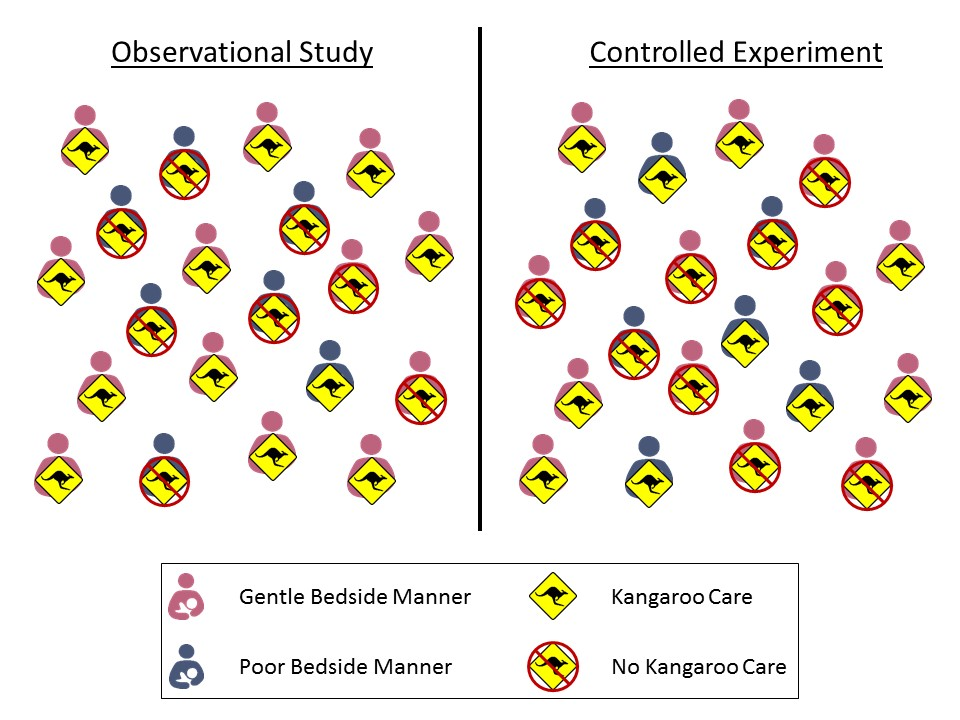
\includegraphics[width=0.8\textwidth,height=\textheight]{./images/Data-Randomization.jpg}

}

\caption{\label{fig-data-randomization}Illustration of the impact of
random assignment in study design. For the observational study, the
treatment groups are unbalanced. For the controlled experiment, the
treatment groups are balanced.}

\end{figure}%

\begin{tcolorbox}[enhanced jigsaw, breakable, titlerule=0mm, colframe=quarto-callout-tip-color-frame, bottomtitle=1mm, opacityback=0, rightrule=.15mm, toptitle=1mm, arc=.35mm, bottomrule=.15mm, left=2mm, title=\textcolor{quarto-callout-tip-color}{\faLightbulb}\hspace{0.5em}{Big Idea}, leftrule=.75mm, coltitle=black, toprule=.15mm, colbacktitle=quarto-callout-tip-color!10!white, colback=white, opacitybacktitle=0.6]

Randomly assigning subjects to groups balances the groups with respect
to any confounders; that is, the groups being compared are similar.
Therefore, any differences between the two groups can be attributed to
the grouping itself, leading to cause-and-effect conclusions.

\end{tcolorbox}

While controlled experiments are a fantastic study design, we should not
discount the use of observational studies. Consider the Deepwater
Horizon Case Study described in Chapter~\ref{sec-caseDeepwater}; suppose
we are interested in the following question:

\begin{quote}
Is there evidence that volunteers who are directly exposed to oil have
an increased risk of developing adverse respiratory symptoms compared to
those who are not directly exposed to oil?
\end{quote}

The response is whether a volunteer develops adverse respiratory
symptoms; the factor of interest is whether the volunteer has direct
exposure to oil. We could conduct a controlled experiment by randomly
determining which volunteers are assigned to wildlife clean up and which
are assigned to administrative tasks, for example. However, it may be
that volunteer tasks need to be determined by skillset or by greatest
need at the time the person volunteers. It may not be feasible to
randomly assign volunteers to specific positions. Or, it could be that
the data was obtained after the fact; that is, the data is not the
result of a planned study in which case random assignment is not
possible because volunteers self-selected into positions in the past. If
random assignment is not possible, it does not mean the data is useless.
But, it does mean we will need to be sure we acknowledge, and
potentially address, the potential confounding when performing the
analysis and discussing the results.

The big idea is that in order to make causal conclusions, we must be
able to state that the groups being compared are balanced with respect
to any potential confounders; random assignment is one technique for
accomplishing this.

\chapter{Presenting the Evidence (Summarizing
Data)}\label{sec-summaries}

If you open any search engine and look up ``data visualization,'' you
will quickly be overwhelmed by a host of pages, texts, and software
filled with tools for summarizing your data. Here is the bottom line: a
good visualization is one that helps you answer your question of
interest. It is both that simple and that complicated.

\begin{tcolorbox}[enhanced jigsaw, breakable, titlerule=0mm, colframe=quarto-callout-important-color-frame, bottomtitle=1mm, opacityback=0, rightrule=.15mm, toptitle=1mm, arc=.35mm, bottomrule=.15mm, left=2mm, title=\textcolor{quarto-callout-important-color}{\faExclamation}\hspace{0.5em}{Fundamental Idea III}, leftrule=.75mm, coltitle=black, toprule=.15mm, colbacktitle=quarto-callout-important-color!10!white, colback=white, opacitybacktitle=0.6]

The use of data for decision making requires that the data be summarized
and presented in ways that address the question of interest and
represent the variability present.

\end{tcolorbox}

Whether simple or complex, all graphical and numerical summaries should
help turn the data into usable information. Pretty pictures for the sake
of pretty pictures are not helpful. In this chapter, we will consider
various simple graphical and numerical summaries to help build a case
for addressing the question of interest. The majority of the chapter is
focused on summarizing a single variable; more complex graphics are
presented in future chapters within a context that requires them.

\section{Characteristics of a Distribution (Summarizing a Single
Variable)}\label{characteristics-of-a-distribution-summarizing-a-single-variable}

Remember that because of \emph{variability}, the key to asking good
questions is to not ask questions about individual values but to
characterize the underlying \emph{distribution} (see
Definition~\ref{def-distribution}). Therefore, characterizing the
underlying distribution is also the key to a good visualization or
numeric summary. For the Deepwater Horizon Case Study described in
Chapter~\ref{sec-caseDeepwater}, the response (whether a volunteer
experienced adverse respiratory symptoms) is categorical. As we stated
previously, summarizing the distribution of a categorical variable
reduces to showing the proportion of individual subjects that fall into
each of the various groups defined by the categorical variable.
Figure~\ref{fig-summaries-deepwater-barchart}) displays a \emph{bar
chart} summarizing the rate of respiratory symptoms for volunteers
cleaning wildlife.

\begin{figure}

\centering{

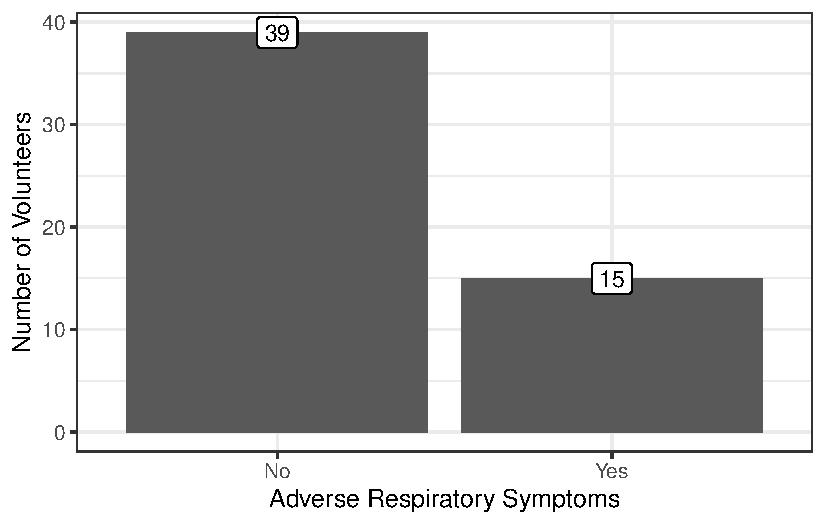
\includegraphics[width=0.8\textwidth,height=\textheight]{./images/fig-summaries-deepwater-barchart-1.pdf}

}

\caption{\label{fig-summaries-deepwater-barchart}Frequency of adverse
respiratory symptoms for volunteers cleaning wildlife following the
Deepwater Horizon oil spill.}

\end{figure}%

In general, it does not matter whether the frequency or the relative
frequencies are reported; however, if the relative frequencies are
plotted, some indication of the sample size should be provided with the
figure, either as an annotation or within the caption. From the above
graphic, we see that nearly 28\% of volunteers assigned to wildlife
experienced adverse respiratory symptoms; the graphic helps address our
question, even if not definitively.

\begin{tcolorbox}[enhanced jigsaw, breakable, titlerule=0mm, colframe=quarto-callout-note-color-frame, bottomtitle=1mm, opacityback=0, rightrule=.15mm, toptitle=1mm, arc=.35mm, bottomrule=.15mm, left=2mm, title=\textcolor{quarto-callout-note-color}{\faInfo}\hspace{0.5em}{Note}, leftrule=.75mm, coltitle=black, toprule=.15mm, colbacktitle=quarto-callout-note-color!10!white, colback=white, opacitybacktitle=0.6]

When you are summarizing only categorical variables, a bar chart is
sufficient. Statisticians tend to agree that bar charts are preferable
to pie charts (see
\href{https://www.perceptualedge.com/articles/visual_business_intelligence/save_the_pies_for_dessert.pdf}{this
whitepaper} and
\href{http://www.storytellingwithdata.com/blog/2014/06/alternatives-to-pies}{this
blog} for further explanation).

\end{tcolorbox}

While a single type of graphic (bar charts) are helpful for looking at
categorical data, summarizing the distribution of a numeric variable
requires a bit more thought. Consider the following example.

\begin{example}[Paper
Strength]\protect\hypertarget{exm-summaries-paper}{}\label{exm-summaries-paper}

While electronic records have become the predominant means of storing
information, we do not yet live in a paperless society. Paper products
are still used in a variety of applications ranging from printing
reports and photography to packaging and bathroom tissue. In
manufacturing paper for a particular application, the strength of the
resulting paper product is a key characteristic.

There are several metrics for the strength of paper. A conventional
metric for assessing the inherent (not dependent upon the physical
characteristics, such as the weight of the paper, which might have an
effect) strength of paper is the \emph{breaking length}. This is the
length of a paper strip, if suspended vertically from one end, that
would break under its own weight. Typically reported in kilometers, the
breaking length is computed from other common measurements. For more
information on paper strength measurements and standards, see the
following website: \url{http://www.paperonweb.com}

A study was conducted at the University of Toronto to investigate the
relationship between pulp fiber properties and the resulting paper
properties (Lee 1992). The breaking length was obtained for each of the
62 paper specimens, the first 5 measurements of which are shown in
Table~\ref{tbl-summaries-paper-table}. The complete dataset is available
online at the following website:
\url{https://vincentarelbundock.github.io/Rdatasets/doc/robustbase/pulpfiber.html}

While there are several questions one might ask with the available data,
here we are primarily interested in characterizing the breaking length
of these paper specimens.

\end{example}

\begin{table}

\caption{\label{tbl-summaries-paper-table}Breaking length (km) for first
5 specimens in the Paper Strength study.}

\centering{

\centering
\begin{tabular}[t]{rr}
\toprule
Specimen & Breaking Length\\
\midrule
\cellcolor{gray!10}{1} & \cellcolor{gray!10}{21.312}\\
2 & 21.206\\
\cellcolor{gray!10}{3} & \cellcolor{gray!10}{20.709}\\
4 & 19.542\\
\cellcolor{gray!10}{5} & \cellcolor{gray!10}{20.449}\\
\bottomrule
\end{tabular}

}

\end{table}%

Figure~\ref{fig-summaries-paper-dotplot} presents the breaking length
for all 62 paper specimens in the sample through a \emph{dot plot} in
which the breaking length for each observed specimen is represented on a
number line using a single dot.

\begin{figure}

\centering{

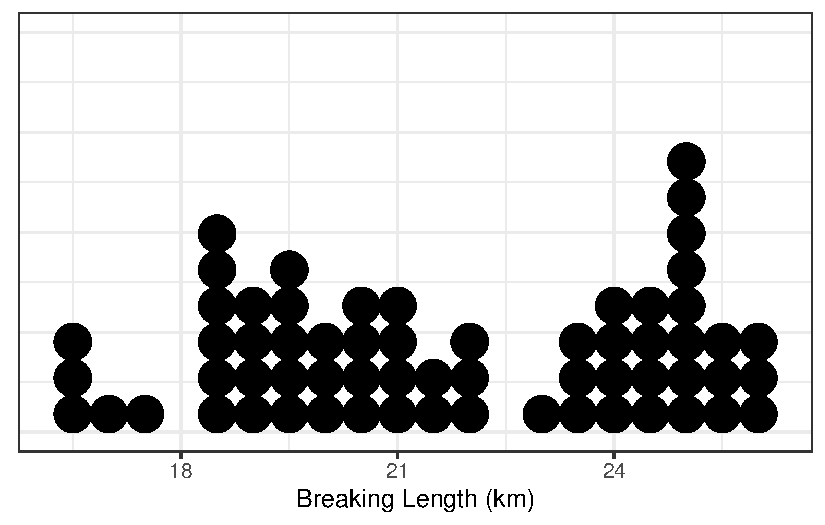
\includegraphics[width=0.8\textwidth,height=\textheight]{./images/fig-summaries-paper-dotplot-1.pdf}

}

\caption{\label{fig-summaries-paper-dotplot}Breaking Length (km) for 62
paper specimens.}

\end{figure}%

With any graphic, we tend to be drawn to three components:

\begin{itemize}
\tightlist
\item
  \emph{where} the values tend to be,
\item
  \emph{how tightly} the values tend to be clustered there, and
\item
  \emph{the way} the values tend to cluster.
\end{itemize}

Notice that about half of the paper specimens in the sample had a
breaking length longer than 21.26 km. Only about 25\% of paper specimens
had a breaking length less than 19.33 km. These are measures of
\emph{location}. In particular, these are known as \textbf{percentiles},
of which the \textbf{median}, \textbf{first quartile} and \textbf{third
quartile} are commonly used examples.

\begin{definition}[Percentile]\protect\hypertarget{def-percentile}{}\label{def-percentile}

The \(k\)-th percentile is the value \(q\) such that \(k\)\% of the
values in the distribution are less than or equal to \(q\). For example,

\begin{itemize}
\tightlist
\item
  25\% of values in a distribution are less than or equal to the 25-th
  percentile (known as the ``first quartile'' and denoted \(Q_1\)).
\item
  50\% of values in a distribution are less than or equal to the 50-th
  percentile (known as the ``median'').
\item
  75\% of values in a distribution are less than or equal to the 75-th
  percentile (known as the ``third quartile'' and denoted \(Q_3\)).
\end{itemize}

\end{definition}

The \textbf{average} is also a common measure of location. The breaking
length of a paper specimen is 21.72 km, on average. In this case, the
average breaking length and median breaking length are very close; this
need not be the case. The average is not describing the ``center'' of
the data in the same way as the median; they capture different
properties.

\begin{definition}[Average]\protect\hypertarget{def-average}{}\label{def-average}

Also known as the ``mean,'' this measure of location represents the
balance point for the distribution. If \(x_i\) represents the \(i\)-th
value of the variable \(x\) in the sample, the sample mean is typically
denoted by \(\bar{x}\).

For a sample of size \(n\), it is computed by
\[\bar{x} = \frac{1}{n}\sum_{i=1}^{n} x_i.\]

When referencing the average for a population, the mean is also called
the ``Expected Value,'' and is often denoted by \(\mu\).

\end{definition}

Clearly, the breaking length is not equivalent for all paper specimens;
that is, there is variability in the measurements. Measures of
\emph{spread} quantify the variability of values within a distribution.
Common examples include the \textbf{standard deviation} (related to
\textbf{variance}) and \textbf{interquartile range}. For the Paper
Strength example, the breaking length varies with a standard deviation
of 2.88 km; the interquartile range for the breaking length is 5.2 km.

The standard deviation is often reported more often than the variance
since it is on the same scale as the original data; however, as we will
see later, the variance is useful from a mathematical perspective for
derivations. Neither of these values has a natural interpretation;
instead, larger values of these measures simply indicate a higher degree
of variability in the data.

\begin{definition}[Variance]\protect\hypertarget{def-variance}{}\label{def-variance}

A measure of spread, this roughly captures the average distance values
in the distribution are from the mean.

For a sample of size \(n\), it is computed by
\[s^2 = \frac{1}{n-1}\sum_{i=1}^{n} \left(x_i - \bar{x}\right)^2\]

where \(\bar{x}\) is the sample mean and \(x_i\) is the \(i\)-th value
in the sample. The division by \(n-1\) instead of \(n\) removes bias in
the statistic.

The symbol \(\sigma^2\) is often used to denote the variance in the
population.

\end{definition}

\begin{definition}[Standard
Deviation]\protect\hypertarget{def-standard-deviation}{}\label{def-standard-deviation}

A measure of spread, this is the square root of the variance.

\end{definition}

\begin{definition}[Interquartile
Range]\protect\hypertarget{def-interquartile-range}{}\label{def-interquartile-range}

Often abbreviated as IQR, this is the distance between the first and
third quartiles. This measure of spread indicates the range over which
the middle 50\% of the data is spread.

\end{definition}

\begin{tcolorbox}[enhanced jigsaw, breakable, titlerule=0mm, colframe=quarto-callout-note-color-frame, bottomtitle=1mm, opacityback=0, rightrule=.15mm, toptitle=1mm, arc=.35mm, bottomrule=.15mm, left=2mm, title=\textcolor{quarto-callout-note-color}{\faInfo}\hspace{0.5em}{Note}, leftrule=.75mm, coltitle=black, toprule=.15mm, colbacktitle=quarto-callout-note-color!10!white, colback=white, opacitybacktitle=0.6]

The IQR is often incorrectly reported as the interval
\(\left(Q_1, Q_3\right)\). The IQR is actually the width of this
interval, not the interval itself.

\end{tcolorbox}

The measures we have discussed so far are illustrated in
Figure~\ref{fig-summaries-summaries}. While some authors suggest the
summaries you choose to report depend on the shape of the distribution,
we argue that it is best to report the values that align with the
question of interest. It is the question that should be shaped by the
beliefs about the underlying distribution.

\begin{figure}

\centering{

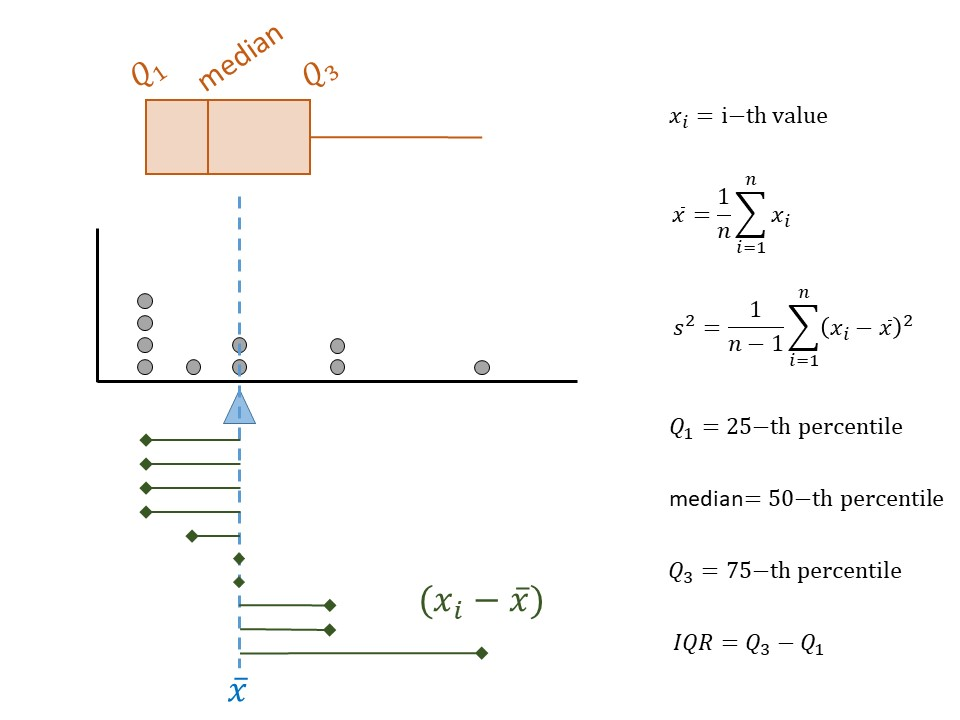
\includegraphics[width=0.8\textwidth,height=\textheight]{./images/Summaries-Summaries.jpg}

}

\caption{\label{fig-summaries-summaries}Illustration of measures of
location and spread for a distribution of values.}

\end{figure}%

Finally, consider the \emph{shape} of the distribution of breaking
length we have observed. The breaking length tends to be clustered in
two locations; we call this \emph{bimodal} (each mode is a ``hump'' in
the distribution). Other terms used to describe the shape of a
distribution are \emph{symmetric} and \emph{skewed}. Symmetry refers to
cutting a distribution in half (at the median) and the lower half being
a mirror image of the upper half; skewed distributions are those which
are not symmetric.

Observe that the dot plot above gives us some idea of the location,
spread, and shape of the distribution, in a way that the table of values
could not. This makes it a useful graphic as it is characterizing the
\textbf{distribution of the sample} we have observed. This is one of the
four components of what we call the \emph{Distributional Quartet}.

\begin{definition}[Distribution of the
Sample]\protect\hypertarget{def-distribution-sample}{}\label{def-distribution-sample}

The pattern of variability in the observed values of a variable.

\end{definition}

When the sample is not large, a dot plot is reasonable. Other common
visualizations for a single numeric variable include:

\begin{itemize}
\tightlist
\item
  \emph{jitter plot}: similar to a dot plot, each value observed is
  represented by a dot; the dots are ``jittered'' (shifted randomly) in
  order to avoid over-plotting when many subjects share the same value
  of the response.
\item
  \emph{box plot}: a visual depiction of five key percentiles; the plot
  includes the minimum, first quartile, median, third quartile, and
  maximum value observed. The quartiles are connected with a box, the
  median cuts the box into two components. Occasionally,
  \textbf{outliers} are denoted on the graphic.
\item
  \emph{histogram}: can be thought of as a grouped dot plot in which
  subjects are ``binned'' into groups of similar values. The height of
  each bin represents the number of subjects falling into that bin.
\item
  \emph{density plot}: a smoothed histogram in which the y-axis has been
  standardized so that the area under the curve has value 1. The y-axis
  is not interpretable directly, but higher values along the y-axis
  indicate that the corresponding values on along the x-axis are more
  likely to occur.
\end{itemize}

\begin{definition}[Outlier]\protect\hypertarget{def-outlier}{}\label{def-outlier}

An individual observation which is so extreme, relative to the rest of
the observations in the sample, that it does not appear to conform to
the same distribution.

\end{definition}

To illustrate these graphics, the breaking length for the Paper Strength
example is summarized using various methods in
Figure~\ref{fig-summaries-univariate}. The latter three visualizations
are more helpful when the dataset is very large and plotting the raw
values actually hides the distribution. There is no right or wrong
graphic; it is about choosing the graphic which addresses the question
and adequately portrays the distribution.

\begin{figure}

\centering{

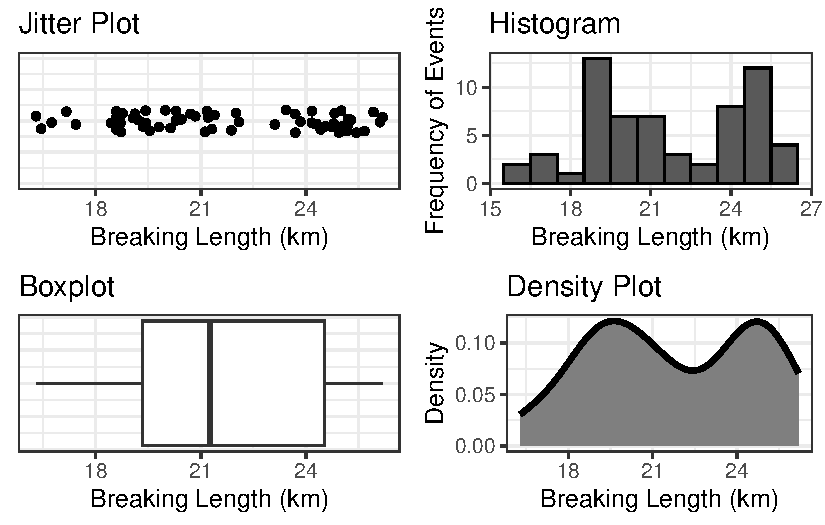
\includegraphics[width=0.8\textwidth,height=\textheight]{./images/fig-summaries-univariate-1.pdf}

}

\caption{\label{fig-summaries-univariate}Four graphical summaries of the
breaking length for the Paper Strength example.}

\end{figure}%

The numeric summaries of a distribution are known as
\textbf{statistics}. While parameters characterize a variable at the
population level, statistics characterize a variable at the sample
level.

\begin{definition}[Statistic]\protect\hypertarget{def-statistic}{}\label{def-statistic}

Numeric quantity which summarizes the distribution of a variable within
a \emph{sample}.

\end{definition}

Why would we compute numerical summaries in the sample if we are
interested in the population? Remember the goal of this discipline is to
use the sample to say something about the underlying population. As long
as the sample is representative, the distribution of the sample should
reflect the \textbf{distribution of the population}; therefore,
summaries of the sample should be close to the analogous summaries of
the population (statistics estimate their corresponding parameters). Now
we see the real importance of having a representative sample; it allows
us to say that what we observe in the sample is a good proxy for what is
happening in the population.

\begin{definition}[Distribution of the
Population]\protect\hypertarget{def-distribution-population}{}\label{def-distribution-population}

The pattern of variability in values of a variable at the population
level. Generally, this is impossible to know, but we might model it.

\end{definition}

Statistics being a proxy for the corresponding parameter implies the
mean in the sample should approximate (estimate) the mean in the
population; the standard deviation of the sample should estimate the
standard deviation in the population; and, the shape of the sample
should approximate the shape of the population, etc. The sample is
acting as a representation in all possible ways of the population.

\begin{tcolorbox}[enhanced jigsaw, breakable, titlerule=0mm, colframe=quarto-callout-tip-color-frame, bottomtitle=1mm, opacityback=0, rightrule=.15mm, toptitle=1mm, arc=.35mm, bottomrule=.15mm, left=2mm, title=\textcolor{quarto-callout-tip-color}{\faLightbulb}\hspace{0.5em}{Big Idea}, leftrule=.75mm, coltitle=black, toprule=.15mm, colbacktitle=quarto-callout-tip-color!10!white, colback=white, opacitybacktitle=0.6]

A representative sample reflects the population; therefore, we can use
statistics as estimates of the population parameters.

\end{tcolorbox}

\begin{tcolorbox}[enhanced jigsaw, breakable, titlerule=0mm, colframe=quarto-callout-note-color-frame, bottomtitle=1mm, opacityback=0, rightrule=.15mm, toptitle=1mm, arc=.35mm, bottomrule=.15mm, left=2mm, title=\textcolor{quarto-callout-note-color}{\faInfo}\hspace{0.5em}{Note}, leftrule=.75mm, coltitle=black, toprule=.15mm, colbacktitle=quarto-callout-note-color!10!white, colback=white, opacitybacktitle=0.6]

Notation in any discipline is both important and somewhat arbitrary. We
can choose any symbol we want to represent the sample mean. However, it
is convention that we never use \(\bar{x}\) to represent a parameter
like the mean of the population. The symbol \(\bar{x}\) (or \(\bar{y}\),
etc.) represents observed values being averaged together. Since the
values are observed, we must be talking about the sample, and therefore
\(\bar{x}\) represents a statistic. A similar statement could be made
for \(s^2\) (sample variance) compared to \(\sigma^2\) (population
variance).

Again, in reality, the symbols themselves are not important. The
importance is on their representation. Statistics are observed while
parameters are not.

\end{tcolorbox}

\section{Summarizing Relationships}\label{summarizing-relationships}

The summaries discussed above are nice for examining a single variable.
In general, however, research questions of interest typically involve
the relationship between two or more variables. Most graphics are
two-dimensional (though 3-dimensional graphics and even virtual reality
are being utilized now); therefore, summarizing a rich set of
relationships may require the use of both axes as well as color, shape,
size, and even multiple plots in order to tell the right story. We will
explore these various features in upcoming units of the text. Here, we
focus on the need to tell a story that answers the question of interest
instead of getting lost in making a graphic. Consider the following
question from the Deepwater Horizon Case Study described in
\#sec-caseDeepwater:

\begin{quote}
What is the increased risk of developing adverse respiratory symptoms
for volunteers cleaning wildlife compared to those volunteers who do not
have direct exposure to oil?
\end{quote}

Consider the graphic in Figure~\ref{fig-summaries-bad-barchart}; this is
\emph{not} a useful graphic. While it compares the number of volunteers
with symptoms in each group, we cannot adequately address the question
because the research question involves comparing the rates for the two
groups; that is, we are lacking a sense of how many volunteers in each
group did not report symptoms.

\begin{figure}

\centering{

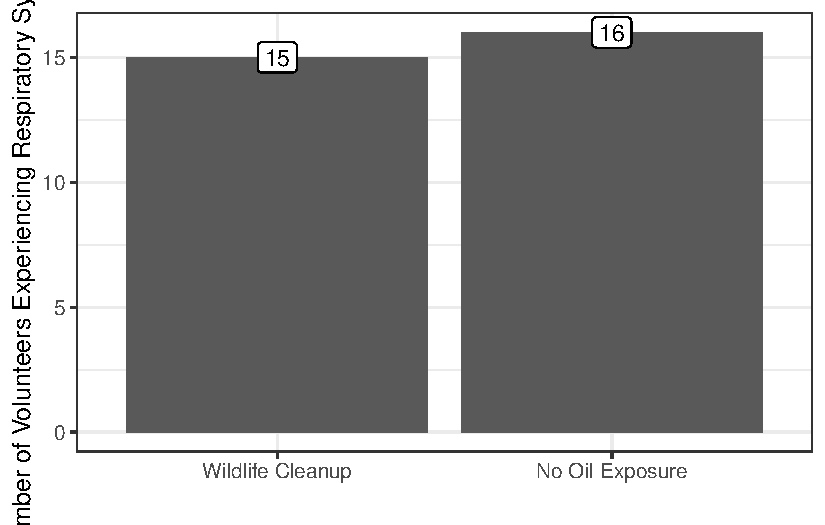
\includegraphics[width=0.8\textwidth,height=\textheight]{./images/fig-summaries-bad-barchart-1.pdf}

}

\caption{\label{fig-summaries-bad-barchart}Illustration of a poor
graphic; the graphic does not give us a sense of the rate within each
group at which volunteers reported symptoms.}

\end{figure}%

Instead, Figure~\ref{fig-summaries-good-barchart} compares the rates
within each group. Note that the graphic is still reporting frequency
along the y-axis; that was not the primary problem with
Figure~\ref{fig-summaries-bad-barchart}. However, by reporting
frequencies for both those with respiratory symptoms and those without,
we get a sense of the relative frequency with which respiratory symptoms
occur.

\begin{figure}

\centering{

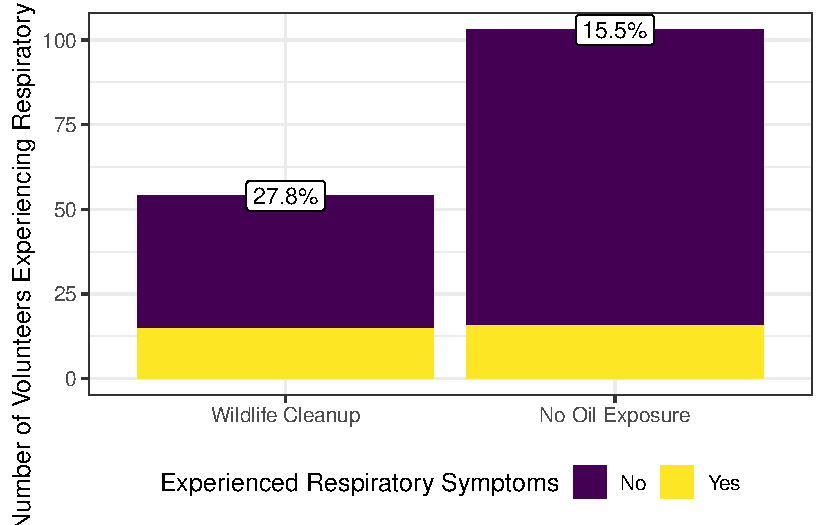
\includegraphics[width=0.8\textwidth,height=\textheight]{./images/fig-summaries-good-barchart-1.pdf}

}

\caption{\label{fig-summaries-good-barchart}Comparison of the rate of
adverse respiratory symptoms among volunteers assigned to different
tasks.}

\end{figure}%

From the graphic, it becomes clear that within the sample a higher
fraction of volunteers cleaning wildlife experienced adverse symptoms
compared with those without oil exposure. In fact, volunteers cleaning
wildlife were 1.79 times more likely to experience adverse respiratory
symptoms.

The key to a good summary is understanding the question of interest and
addressing this question through a useful characterization of the
variability.

\chapter{Assessing the Evidence (Quantifying the Variability in
Estimates)}\label{sec-samplingdistns}

Again, the goal of statistical inference is to use the sample as a
snapshot of the underlying population
(Figure~\ref{fig-basics-statistical-process}). There are generally three
reasons people distrust this process:

\begin{enumerate}
\def\labelenumi{\arabic{enumi}.}
\tightlist
\item
  Fear that the sample does not represent what is going on in the
  population.
\item
  Fear that we cannot make a conclusion with a sample of size \(n\)
  (wanting more data).
\item
  Fear that one study is not enough to make a conclusion.
\end{enumerate}

We have already tackled the first fear in Chapter~\ref{sec-data}; if we
are to trust statistical results, we must collect data that is
representative of the underlying population. The second and third fears
above are tied together, though maybe not obviously. Before launching
into a slightly more formal discussion, consider the following thought
experiment.

\begin{example}[Free
Throws]\protect\hypertarget{exm-samplingdistns-free-throws}{}\label{exm-samplingdistns-free-throws}

Your friend Dave lives for his Wednesday ``pick-up'' basketball games at
the gym. One afternoon, while waiting for a few more players to arrive
Dave shoots 10 free throws, of which he makes 3.

\end{example}

While Dave only exhibited a 30\% success rate from the free throw line
in this sample, we imagine no one is ready to claim \emph{definitively}
that Dave has a 30\% success rate from the free throw line overall. So,
what can we say? Well, if this set of 10 free throws is representative
of Dave's free throw performance, then we would say that 30\% is an
\emph{estimate} for his success rate; that is, the statistic 30\% is a
good guess at the unknown parameter (overall success rate). There are
two ways we might improve our ``trust'' in this estimate. First, we
might consider a larger sample size (make Dave shoot more free throws);
let's continue along these lines for a moment.

\begin{example}[Free Throws
(Cont.)]\protect\hypertarget{exm-samplingdistns-free-throws2}{}\label{exm-samplingdistns-free-throws2}

Joe has also been waiting for a few more players to arrive; however, Joe
shoots 100 free throws (clearly he has more time on his hands) of which
he makes 30.

\end{example}

Again, we probably wouldn't claim \emph{definitively} that Joe has a
30\% success rate from the free throw line overall. And again, assuming
this set of 100 free throws is representative of his overall
performance, we would say 30\% is an \emph{estimate} for his success
rate. But, we might also say we have more ``trust'' in our guess for
Joe's overall performance compared with our guess for Dave's. The more
shots we observe, the more we seem to ``trust'' our estimate. This idea
is known as the \textbf{Law of Large Numbers}.

\begin{definition}[Law of Large
Numbers]\protect\hypertarget{def-lln}{}\label{def-lln}

For our purposes, the Law of Large Numbers essentially says that as a
sample size gets infinitely large, a statistic will become arbitrarily
close (extremely good approximation) of the parameter it estimates.

\end{definition}

There are two drawbacks with the Law of Large Numbers. First, it does
not tell us how ``close'' a statistic is to the parameter for any
specific sample size; second, we cannot take an infinitely large sample.
For our thought experiment, it is probably not feasible to have Dave or
Joe shoot thousands of free throws, for example. Our goal then becomes
to somehow quantify the ``trust'' we have in our estimates \emph{given
the sample size we have available}. That is, given that we only saw Dave
shoot 10 free throws, can we quantify our ``trust'' in that 30\%
estimate of his free throw success? We need some way of measuring
``trust,'' and we do that through a notion of statistical
``confidence.''

\begin{tcolorbox}[enhanced jigsaw, breakable, titlerule=0mm, colframe=quarto-callout-tip-color-frame, bottomtitle=1mm, opacityback=0, rightrule=.15mm, toptitle=1mm, arc=.35mm, bottomrule=.15mm, left=2mm, title=\textcolor{quarto-callout-tip-color}{\faLightbulb}\hspace{0.5em}{Big Idea}, leftrule=.75mm, coltitle=black, toprule=.15mm, colbacktitle=quarto-callout-tip-color!10!white, colback=white, opacitybacktitle=0.6]

In statistics, our ``trust'' is tied to the estimate's repeatability; we
ask the question ``if we were to repeat the study, how much would we
expect our estimate to change?''

\end{tcolorbox}

We will formalize the notion of statistical confidence shortly, but for
now, linking our trust in an estimate to its repeatability gets at the
last fear. We know that if we repeat a study, the results will change;
our job is to quantify (keeping the sample size in mind) the degree to
which the results will change. That is, we need to quantify the
\emph{variability} in the estimate across repeated studies (known as
sampling variability; we told you statistics was all about variability).
This is characterized by the \textbf{sampling distribution}.

\begin{definition}[Sampling
Distribution]\protect\hypertarget{def-sampling-distribution}{}\label{def-sampling-distribution}

The distribution of a \emph{statistic} across repeated samples (of the
same size) from the population.

\end{definition}

This is perhaps the most important of the \emph{Distributional Quartet};
it is the holy grail of statistical inference. Once we have the sampling
distribution, inference is straight-forward.

\begin{tcolorbox}[enhanced jigsaw, breakable, titlerule=0mm, colframe=quarto-callout-important-color-frame, bottomtitle=1mm, opacityback=0, rightrule=.15mm, toptitle=1mm, arc=.35mm, bottomrule=.15mm, left=2mm, title=\textcolor{quarto-callout-important-color}{\faExclamation}\hspace{0.5em}{Fundamental Idea IV}, leftrule=.75mm, coltitle=black, toprule=.15mm, colbacktitle=quarto-callout-important-color!10!white, colback=white, opacitybacktitle=0.6]

Variability is inherent in any process, and as a result, our estimates
are subject to sampling variability. However, these estimates often vary
across samples in a predictable way; that is, they have a distribution
that can be modeled.

\end{tcolorbox}

\section{Conceptualizing the Sampling
Distribution}\label{conceptualizing-the-sampling-distribution}

The sampling distribution of a statistic is one of the most fundamental,
and yet one of the most abstract, concepts in statistics. Its name is
even confusing; the ``distribution of the sample''
(Definition~\ref{def-distribution-sample}) and the ``sampling
distribution'' (Definition~\ref{def-sampling-distribution}) use similar
words but represent two different things. Before we discuss the utility
of the sampling distribution, we first focus on making it a bit more
tangible.

For the Deepwater Horizon Case Study discussed in
Chapter~\ref{sec-caseDeepwater}, consider the following question:

\begin{quote}
What proportion of volunteers assigned to clean wildlife develop adverse
respiratory symptoms?
\end{quote}

In the sample, we observed 15 out of 54 such volunteers (27.8\% or a
proportion of 0.278). This proportion is a good estimate of the rate of
adverse symptoms in the population (assuming the sample is
representative, of course).

Now, imagine randomly selecting 54 \emph{new} volunteers from the
population (repeating the study). For this new sample, it would be
possible to determine the fraction of volunteers that experienced
adverse symptoms; we would expect this value to be a bit different than
what we obtained in the first sample since the two samples consist of
different subjects. Since this second sample is also representative,
however, it also provides a good estimate of the parameter. That is, we
now have two good estimates of the same parameter.

Now, we could take a third random sample of 54 volunteers and compute
the fraction in this third sample which experienced adverse symptoms.
This third sample also provides a good (and potentially unique) estimate
of the parameter. In fact, we could continue this process \(m\) times,
for some large number \(m\), as illustrated in
Figure~\ref{fig-samplingdistns-sampling-distribution}).

\begin{figure}

\centering{

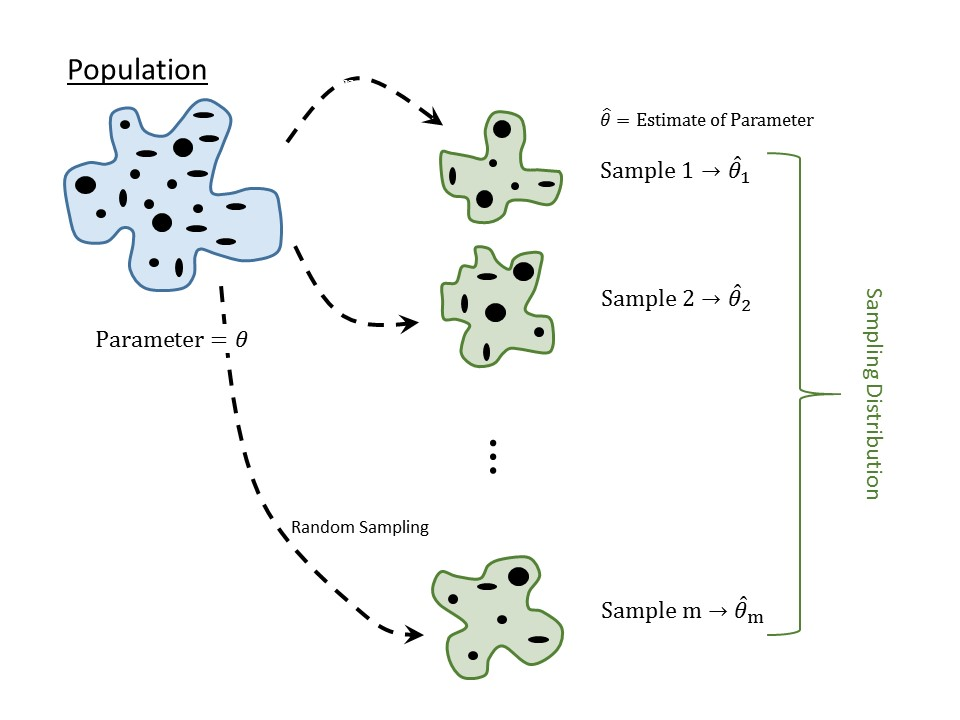
\includegraphics[width=0.8\textwidth,height=\textheight]{./images/SamplingDistns-Sampling-Distribution.jpg}

}

\caption{\label{fig-samplingdistns-sampling-distribution}Illustration of
repeatedly sampling from a population.}

\end{figure}%

Consider what we are describing. With each representative sample, we
have constructed an estimate of the parameter. What we have kept from
each replicate sample is \emph{not} the values of the variables
themselves (whether the volunteers experienced adverse respiratory
symptoms); instead, we have retained the \emph{statistic} from each of
\(m\) completely different studies. So, which of these \(m\) estimates
do we trust? \emph{All of them.} Since each sample is representative of
the population, each estimate is a good (not perfect) estimate of the
parameter. Since we have all these estimates, we should think about what
information they provide. In fact, there is information not only in what
these estimates are but in how different they are from one another.
Describing the way in which these estimates change from one sample to
another is the sampling distribution.

Notice that the sampling distribution is not describing a variable from
our study; it is describing a \emph{statistic}. In order to construct a
sampling distribution, we go through the following steps:

\begin{enumerate}
\def\labelenumi{\arabic{enumi}.}
\tightlist
\item
  Take a sample; record variables of interest.
\item
  Compute the statistic which estimates the parameter and retain this
  value.
\item
  Repeat steps 1 and 2 a large number of times.
\item
  Examine the statistics collected.
\end{enumerate}

So, the sampling distribution is not a plot of the raw values of a
variable on individual subjects but a plot of statistics which summarize
entire samples. That is, the unit of observation has changed in this
distribution. While a sample consists of individual subjects from the
population, the sampling distribution consists of individual samples
from the population.

\begin{tcolorbox}[enhanced jigsaw, breakable, titlerule=0mm, colframe=quarto-callout-tip-color-frame, bottomtitle=1mm, opacityback=0, rightrule=.15mm, toptitle=1mm, arc=.35mm, bottomrule=.15mm, left=2mm, title=\textcolor{quarto-callout-tip-color}{\faLightbulb}\hspace{0.5em}{Big Idea}, leftrule=.75mm, coltitle=black, toprule=.15mm, colbacktitle=quarto-callout-tip-color!10!white, colback=white, opacitybacktitle=0.6]

Re-read the description of a sampling distribution several times, and
return to it often as you read through the text. It takes a while for
this to sink in, but if you truly grasp this one concept, the remainder
of statistical inference becomes much more accessible.

\end{tcolorbox}

\section{Example of a Sampling
Distribution}\label{example-of-a-sampling-distribution}

Since this idea is so critical to grasping statistical inference, we are
going to walk through the process of generating a sampling distribution
for a known data generating process.

\phantomsection\label{ex-samplingdistns-dice}
\section{Dice Experiment}\label{dice-experiment}

Consider an ordinary six-sided die; we are interested in the proportion
of times that rolling the die will result in a 1. Putting this in the
language of the statistics, we have the following:

\begin{itemize}
\tightlist
\item
  The \emph{population} of interest is all rolls of the die. Notice that
  this population is infinitely large as we could roll the die forever.
\item
  The \emph{variable} is the resulting value from the roll. Since this
  can take on only one of six values, this is a categorical variable.
\item
  The \emph{parameter} of interest is the proportion of rolls that
  result in a 1.
\end{itemize}

Our goal is to construct the sampling distribution of the \emph{sample
proportion} of rolls that result in a 1 when the die is rolled 20 times.

What makes this example unique is that we know the value of the
parameter. Because of the physical properties of a die, we know that the
probability a roll results in a 1 is \(\theta = 1/6\). So, statistical
inference is not needed here. This example simply provides a vehicle for
studying sampling distributions. Also, before going on, notice that the
sampling distribution is for the statistic (the \emph{sample
proportion}) and not the parameter; and, it is constructed for a fixed
sample size (in this case, \(n = 20\) rolls). Going back to the steps
for creating a sampling distribution described in the previous section,
we have the following steps:

\begin{enumerate}
\def\labelenumi{\arabic{enumi}.}
\tightlist
\item
  Roll a die 20 times, each time recording the resulting value.
\item
  Compute the proportion of times (out of the 20) the resulting value
  was a 1 and retain this value.
\item
  Repeat steps 1 and 2 a large number of times (let's say 500).
\item
  Plot the resulting values; there should be 500 proportions that we are
  keeping.
\end{enumerate}

Notice that we are actually rolling a die 10000 times (20 rolls repeated
500 times); we only keep 500 values (one proportion for each set of 20
rolls). This is something you could physically do at home. For example,
the first sample might look like that in
Figure~\ref{fig-samplingdistns-dice-example}.

\begin{figure}

\centering{

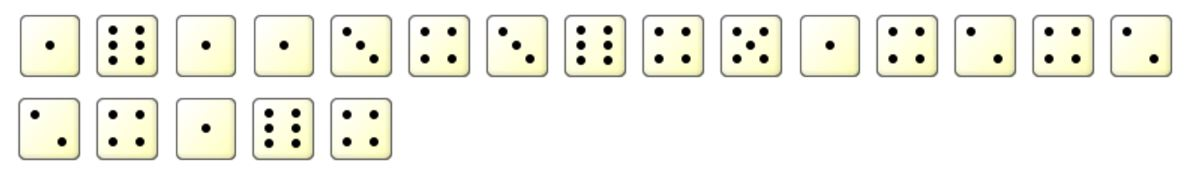
\includegraphics[width=0.8\textwidth,height=\textheight]{./images/SamplingDistns-Dice-Example.jpg}

}

\caption{\label{fig-samplingdistns-dice-example}Potential sample from
rolling a die 20 times.}

\end{figure}%

For this particular sample, the proportion in the sample (our statistic
of interest) would be 0.25 (\(5/20\)). That is the statistic we would
record. We then repeat this 499 more times. You could try a few out
yourself using \href{https://www.random.org/dice/?num=20}{an online
simulator}. Figure~\ref{fig-samplingdistns-dice-dotplot} shows the
resulting proportions for when we simulated this process with 500
samples, each sample consisting of 20 rolls.

\begin{figure}

\centering{

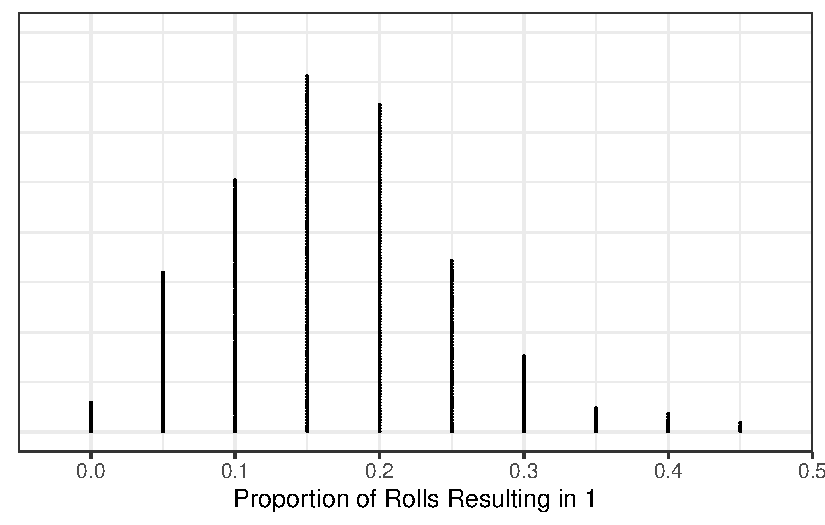
\includegraphics[width=0.8\textwidth,height=\textheight]{./images/fig-samplingdistns-dice-dotplot-1.pdf}

}

\caption{\label{fig-samplingdistns-dice-dotplot}Sampling distribution
for the proportion of 20 rolls of a die which result in a 1. The
distribution is based on repeating the sampling process 500 times.}

\end{figure}%

With modern computing power, there is no need to restrain ourselves to
repeating the study 500 times. A simple computer program could replicate
rolling the study (20 rolls of a die) thousands of times.
Figure~\ref{fig-samplingdistns-dice-histogram} is the sampling
distribution for the proportion of rolls that result in a 1 based on a
sample of size 20, repeating the study 50000 times.

\begin{figure}

\centering{

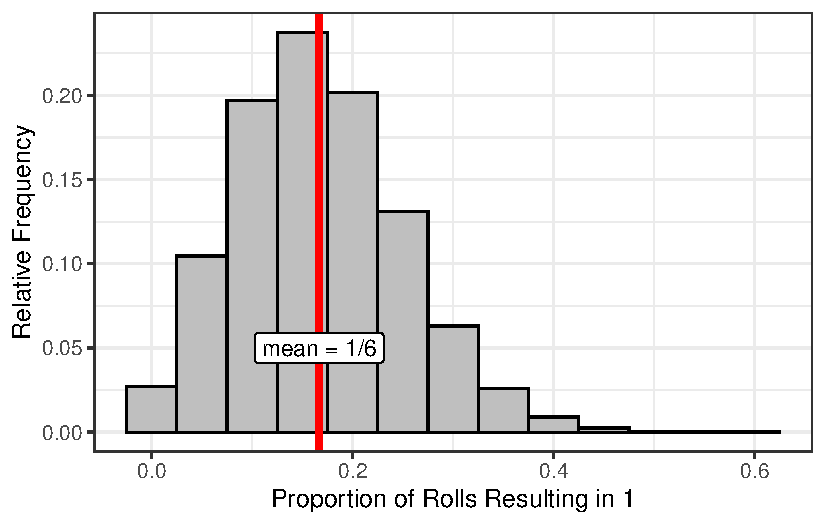
\includegraphics[width=0.8\textwidth,height=\textheight]{./images/fig-samplingdistns-dice-histogram-1.pdf}

}

\caption{\label{fig-samplingdistns-dice-histogram}Sampling distribution
for the proportion of 20 rolls of a die which result in a 1. The
distribution is based on repeating the sampling process 50000 times.}

\end{figure}%

\begin{tcolorbox}[enhanced jigsaw, breakable, titlerule=0mm, colframe=quarto-callout-warning-color-frame, bottomtitle=1mm, opacityback=0, rightrule=.15mm, toptitle=1mm, arc=.35mm, bottomrule=.15mm, left=2mm, title=\textcolor{quarto-callout-warning-color}{\faExclamationTriangle}\hspace{0.5em}{Warning}, leftrule=.75mm, coltitle=black, toprule=.15mm, colbacktitle=quarto-callout-warning-color!10!white, colback=white, opacitybacktitle=0.6]

When looking at a graphical representation of a sampling distribution
(such as Figure~\ref{fig-samplingdistns-dice-histogram}), there is a
tendency to describe the ``data'' in the graphic. However, the use of
the word ``data'' here is inappropriate. We restrict the word ``data''
to refer to information/measurements observed on each subject; this
includes numeric and categorical variables directly measured and any
transformations of these variables.

For example, the total number of credit hours a student has completed is
part of the data observed (quantitative variable). Similarly, using the
total number of credit hours to determine class standing (Freshman,
Sophomore, Junior, Senior) would also be a part of the data observed
(categorical variable).

However, the word ``data'' should not be used to describe the statistics
computed from the sample, or from repeated sampling such as when
constructing a sampling distribution, as these quantities are not
characterizing the individual units under study.

\end{tcolorbox}

Notice that the sampling distribution is centered around the true value
of the parameter (\(\theta = 1/6\)). In general, the sampling
distribution of a statistic, when taken from a random sample, is
centered on the true value of the parameter. This is the unbiased nature
of the data coming out; random samples are representative of the
population. Similarly, note that while no one sample (remember, each
value in the distribution represents a statistic from a sample of 20
values) is perfect, none of the samples produced a statistic which is
really far from the true parameter. That is, a representative sample may
not be perfect, but it will give a \emph{reasonable} estimate of the
parameter. Notice that these properties hold even though we had a
relatively small sample size (only rolling the die \(n = 20\) times).

\begin{tcolorbox}[enhanced jigsaw, breakable, titlerule=0mm, colframe=quarto-callout-tip-color-frame, bottomtitle=1mm, opacityback=0, rightrule=.15mm, toptitle=1mm, arc=.35mm, bottomrule=.15mm, left=2mm, title=\textcolor{quarto-callout-tip-color}{\faLightbulb}\hspace{0.5em}{Big Idea}, leftrule=.75mm, coltitle=black, toprule=.15mm, colbacktitle=quarto-callout-tip-color!10!white, colback=white, opacitybacktitle=0.6]

The size of the sample is not as important as whether it is
representative. A small representative sample is better for making
inference than a large sample which is biased.

\end{tcolorbox}

One of the most useful things about the sampling distribution is that it
gives us an idea of how much we might expect our statistic to change
from one sample to another. Based on
Figure~\ref{fig-samplingdistns-dice-histogram}, we could say that if we
roll a die 20 times, the proportion of rolls which result in a 1 is most
likely to be between 0.05 and 0.30 (so somewhere between 1 and 6 ones
out of the 20 rolls). It would be \emph{extremely} rare to have 12 of
the 20 rolls result in a 1 (notice how small the bar is for a proportion
of 0.6). The sampling distribution is therefore giving us an idea of the
variability in our statistic.

Remember, our goal was to account for the variability in the statistic
(how much it changes from one sample to another) \emph{while accounting
for the sample size}. How is this done? When forming the sampling
distribution, we repeated the study, which included ensuring that for
each replication, we obtained a new sample that \emph{had the same size
as the original sample}. So, the sample size is baked into the sampling
distribution. To see the impact of taking a larger sample, consider
rolling a six-sided die 60 times instead of 20 times. When we build the
sampling distribution, each replication will then involve repeating the
process with 60 new rolls.
Figure~\ref{fig-samplingdistns-dice-histogram2} shows the sampling
distribution of the proportion of 60 rolls which result in a 1, using
50000 replications. Notice that the distribution is still centered on
the true parameter \(\theta = 1/6\). The primary difference between this
figure and the last is that when we increased the sample size, the
sampling distribution narrowed.

\begin{figure}

\centering{

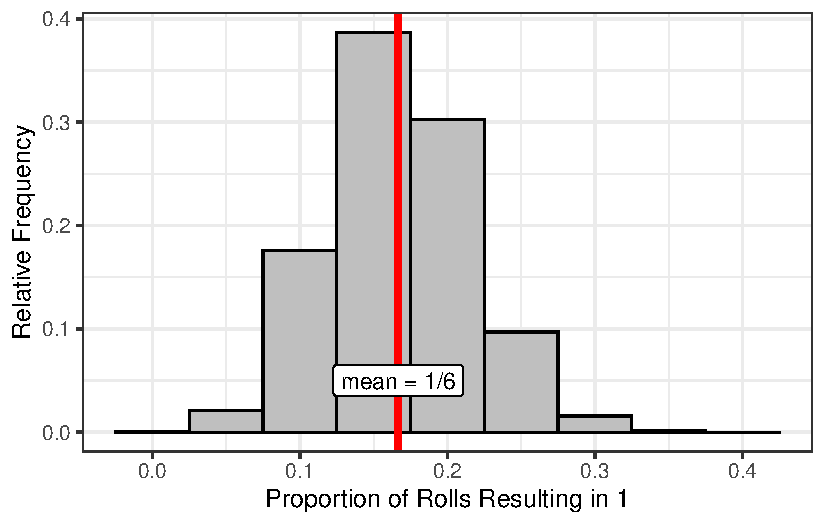
\includegraphics[width=0.8\textwidth,height=\textheight]{./images/fig-samplingdistns-dice-histogram2-1.pdf}

}

\caption{\label{fig-samplingdistns-dice-histogram2}Sampling distribution
for the proportion of 60 rolls of a die which result in a 1. The
distribution is based on repeating the sampling process 50000 times.}

\end{figure}%

We all have this intuition that ``more data is better.'' In truth, we
should say ``more \emph{good} data is better'' since we understand that
having a representative sample is extremely important. With that in
mind, the distinction between Figures
\ref{fig-samplingdistns-dice-histogram} and
\ref{fig-samplingdistns-dice-histogram2} illustrate what we really mean
when we say ``better'' --- the statistic is less variable. We have to be
careful here. We are \textbf{not} saying that the \emph{sample} has less
variability; we are saying the \emph{statistic} has less variability.
That is, we do not expect our estimate to change as much from one sample
to the next. From Figure~\ref{fig-samplingdistns-dice-histogram2}, we
have that if we roll the die 60 times, we expect the proportion of 1's
to be somewhere between 0.1 and 0.25 (somewhere between 6 and 15 ones
out of the 60 show up). The proportion is varying much less from one
sample to the next compared to when we rolled the die only 20 times.

\begin{tcolorbox}[enhanced jigsaw, breakable, titlerule=0mm, colframe=quarto-callout-tip-color-frame, bottomtitle=1mm, opacityback=0, rightrule=.15mm, toptitle=1mm, arc=.35mm, bottomrule=.15mm, left=2mm, title=\textcolor{quarto-callout-tip-color}{\faLightbulb}\hspace{0.5em}{Big Idea}, leftrule=.75mm, coltitle=black, toprule=.15mm, colbacktitle=quarto-callout-tip-color!10!white, colback=white, opacitybacktitle=0.6]

Larger samples result in \emph{statistics} which are less variable. That
is, as the sample size increases, the sampling distribution of a
statistic becomes narrower.

\end{tcolorbox}

\begin{tcolorbox}[enhanced jigsaw, breakable, titlerule=0mm, colframe=quarto-callout-note-color-frame, bottomtitle=1mm, opacityback=0, rightrule=.15mm, toptitle=1mm, arc=.35mm, bottomrule=.15mm, left=2mm, title=\textcolor{quarto-callout-note-color}{\faInfo}\hspace{0.5em}{Note}, leftrule=.75mm, coltitle=black, toprule=.15mm, colbacktitle=quarto-callout-note-color!10!white, colback=white, opacitybacktitle=0.6]

Students often believe that a large sample reduces the variability in
the data. That is not true; a large sample reduces the variability in
the \emph{statistic}.

\end{tcolorbox}

\begin{tcolorbox}[enhanced jigsaw, breakable, titlerule=0mm, colframe=quarto-callout-warning-color-frame, bottomtitle=1mm, opacityback=0, rightrule=.15mm, toptitle=1mm, arc=.35mm, bottomrule=.15mm, left=2mm, title=\textcolor{quarto-callout-warning-color}{\faExclamationTriangle}\hspace{0.5em}{Warning}, leftrule=.75mm, coltitle=black, toprule=.15mm, colbacktitle=quarto-callout-warning-color!10!white, colback=white, opacitybacktitle=0.6]

We repeat a warning here that we stated when introducing the concept of
\emph{bias}. There is a difference between \emph{accuracy} and
\emph{precision}. Generally, \emph{accuracy} refers to location (and
therefore bias); we say an estimate is accurate when it is unbiased.
\emph{Precision} refers to the variability; we say an estimate is more
precise when it has less variability. With regard to sampling
distributions, accuracy refers to the center of the sampling
distribution while precision refers to its spread.

\end{tcolorbox}

We have briefly discussed the center and spread of the sampling
distribution we constructed above. Before leaving this section, a note
on the shape of the sampling distribution is also in order. Note that
for this example, the resulting observations can take on one of only two
values (heads or tails). A bar chart summarizing this distribution (that
of the variable within the \emph{population}) would consist of only two
bars. However, the distribution of the statistic that we record (that
is, the \emph{sampling distribution}) is bell-shaped
(fig-samplingdistns-dice-histogram2). While the sampling distribution
will not always be bell-shaped, it is often the case for the statistics
discussed in this text. The key thing to recognize is that the
distribution of the variable and the distribution of the statistic are
not the same.

\section{Modeling the Sampling
Distribution}\label{modeling-the-sampling-distribution}

Let's return to the Deepwater Horizon Case Study. In particular, suppose
we are trying to address the following question:

\begin{quote}
What proportion of volunteers assigned to clean wildlife develop adverse
respiratory symptoms?
\end{quote}

We have an estimate for this proportion (\(\widehat{p} = 0.278\)) based
on the observed sample. Based on the discussion in the previous section,
we know the sampling distribution of this proportion can help us
quantify the variability in the estimate.
Figure~\ref{fig-samplingdistns-deepwater-histogram} represents the
sampling distribution of this proportion. From the graphic, we would not
expect the proportion of volunteers who experience adverse respiratory
symptoms to move much beyond 0.15 and 0.4 if we were to repeat the
study; it would almost certainly not move beyond 0.1 and 0.5 if we were
to repeat the study.

\begin{figure}

\centering{

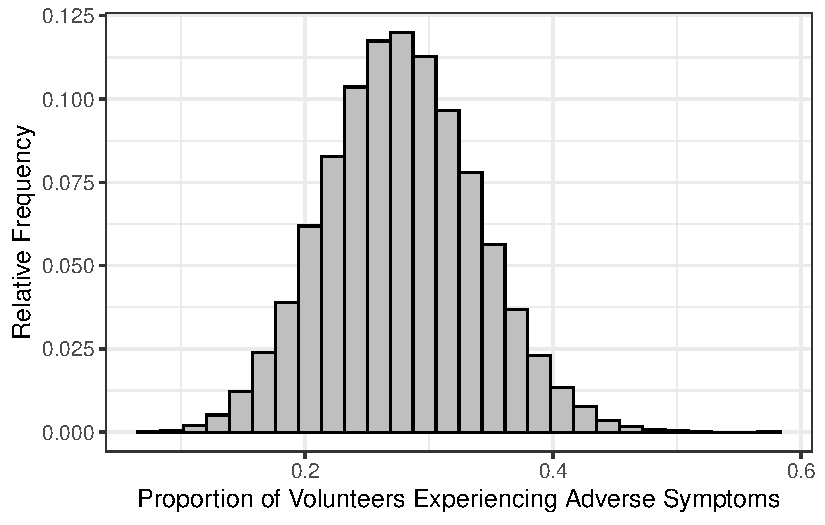
\includegraphics[width=0.8\textwidth,height=\textheight]{./images/fig-samplingdistns-deepwater-histogram-1.pdf}

}

\caption{\label{fig-samplingdistns-deepwater-histogram}Sampling
distribution for the proportion of volunteers assigned to wildlife who
develop adverse symptoms based on a sample of 54 volunteers.}

\end{figure}%

Now, you might ask ``wait, where did this sampling distribution come
from? There is no way you actually repeated the study 50000 times,
right?'' And, you would be right.

In the previous section, we described building the sampling distribution
through repeated sampling. In practice, this is never practical.
Generally, cost is the limiting factor when collecting data; as a
result, we get a single sample to work with. We have essentially argued
that the sampling distribution is critical to making inference, but we
cannot take multiple samples to make it. Where does that leave us? The
answer\ldots modeling. Our goal is to construct a \emph{model} of the
sampling distribution that we can use to make inference.

There are three general techniques for modeling the sampling
distribution of a statistic:

\begin{enumerate}
\def\labelenumi{\arabic{enumi}.}
\tightlist
\item
  Build an empirical model.
\item
  Build an exact analytical model using results from probability theory.
\item
  Build an approximate analytical model using results from theorems
  about limits in probability.
\end{enumerate}

We will focus on the first approach; the latter two approaches are
discussed in Appendix~\ref{sec-app-theory}. Our emphasis in this chapter
is on the conceptual understanding of a sampling distribution and its
model. While these latter two approaches differ in their technique, the
use of the resulting model is the same. We choose to focus on the first
approach because it requires less mathematical background and reinforces
the conceptual understanding of a sampling distribution discussed above.
The idea in constructing an empirical model is to mimic the discussion
above regarding the construction of a sampling distribution. Our
description references Figure~\ref{fig-samplingdistns-bootstrap} often.

We are limited by our resources; because of time and money constraints,
we cannot resample from the population (crossed off resamples in
Figure~\ref{fig-samplingdistns-bootstrap}). So, we pretend for a moment
that our original sample (colored in green in
Figure~\ref{fig-samplingdistns-bootstrap}) is the population. Our idea
is to randomly sample from this original data, creating a
\emph{resample} (colored in orange in
Figure~\ref{fig-samplingdistns-bootstrap}). Forgive the non-technical
terms here, but since the orange ``blob'' is a random sample from the
green ``blob,'' then it is representative of the green blob. Therefore,
if we construct an estimate \(\widehat{\theta}^*\) from the orange blob
(the star denotes a statistic from a resample), then it should be close
to the statistic \(\widehat{\theta}\) from the green blob; but, since
this green blob is representative of the population,
\(\widehat{\theta}\) should be a good estimate of \(\theta\). Therefore,
we have that

\[
\widehat{\theta}^* \approx \widehat{\theta} \approx \theta \Rightarrow \widehat{\theta}^* \approx \theta
\]

That is, each resample produces a statistic which is a good estimate of
the parameter from the underlying population. The benefit here is that
the resamples are taken from the original sample, not the population,
and can therefore be constructed in the computer. And, given today's
computing power, we are not limited by time or money (10000 resamples
can often be taken in a matter of seconds). If you want to see this
process in action, we encourage you to check out the free online app
located at
\url{http://www.lock5stat.com/StatKey/bootstrap_1_cat/bootstrap_1_cat.html}.

\begin{figure}

\centering{

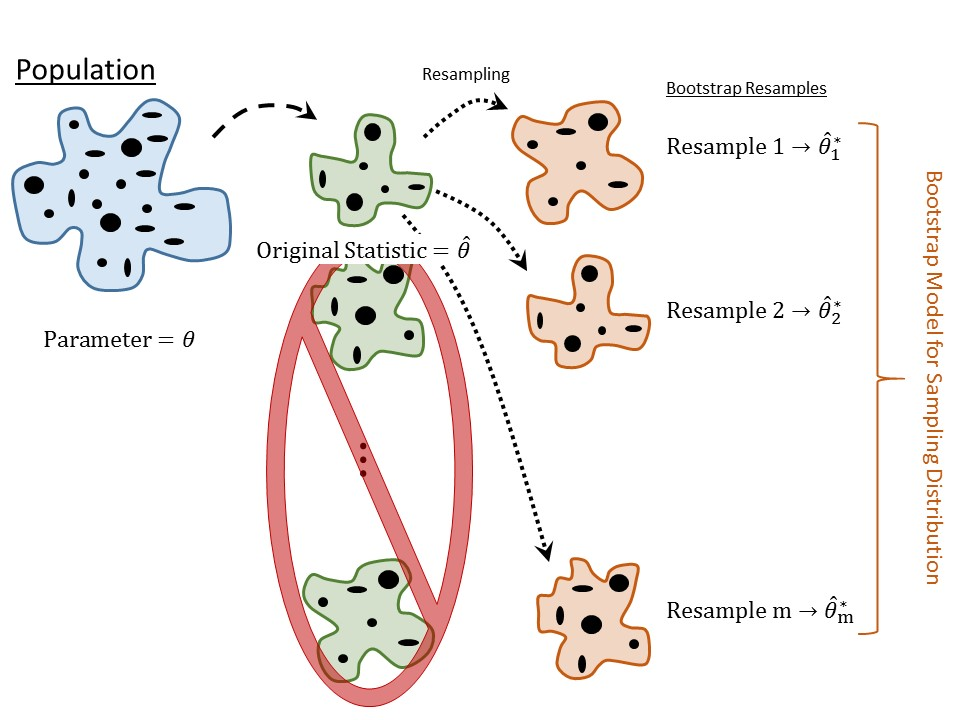
\includegraphics[width=0.8\textwidth,height=\textheight]{./images/SamplingDistns-Bootstrap.jpg}

}

\caption{\label{fig-samplingdistns-bootstrap}Illustration of modeling
the sampling distribution via bootstrapping.}

\end{figure}%

Again, the idea is to mimic in the computer the resampling that we were
unable to do in real life. This process is known as
\textbf{bootstrapping}.

\begin{definition}[Bootstrapping]\protect\hypertarget{def-bootstrap}{}\label{def-bootstrap}

A method of modeling the sampling distribution by repeatedly resampling
from the original data.

\end{definition}

There are actually several variations of bootstrapping; however, for our
purposes currently, we can keep the following details regarding the
implementation in mind:

\begin{enumerate}
\def\labelenumi{\arabic{enumi}.}
\tightlist
\item
  Each resample (known as a \emph{bootstrap resample}) is the same size
  as the original sample.
\item
  Each resample is taken \emph{with replacement}; that means the values
  from the original sample can show up multiple times. Think of ``catch
  and release'' fishing.
\item
  Typically, between 3000 and 10000 bootstrap resamples are taken.
\end{enumerate}

We will avoid actual computation throughout the text, but a quick online
search would provide several resources for implementing the process we
have described (and its many variants) in various computer programming
languages and software packages.

\begin{tcolorbox}[enhanced jigsaw, breakable, titlerule=0mm, colframe=quarto-callout-tip-color-frame, bottomtitle=1mm, opacityback=0, rightrule=.15mm, toptitle=1mm, arc=.35mm, bottomrule=.15mm, left=2mm, title=\textcolor{quarto-callout-tip-color}{\faLightbulb}\hspace{0.5em}{Big Idea}, leftrule=.75mm, coltitle=black, toprule=.15mm, colbacktitle=quarto-callout-tip-color!10!white, colback=white, opacitybacktitle=0.6]

Students often believe that bootstrapping ``creates more data.'' This is
not true. Instead, boostrapping resamples from the existing data. By its
very nature, it takes the limited information in the sample into
account. This highlights the need to have a representative sample when
performing analysis.

\end{tcolorbox}

For the Deepwater Horizon Case Study discussed in
Chapter~\ref{sec-caseDeepwater}, we performed the following steps to
create Figure~\ref{fig-samplingdistns-deepwater-histogram}:

\begin{enumerate}
\def\labelenumi{\arabic{enumi}.}
\tightlist
\item
  Select 54 volunteers at random (with replacement) from the original
  sample of 54 volunteers who had been assigned to clean wildlife.
\item
  For our bootstrap resample, we compute the proportion of those
  individuals who had experienced adverse respiratory symptoms; this is
  our \emph{bootstrap statistic}.
\item
  We repeated steps 1 and 2 several thousand times, retaining the
  bootstrap statistics from each bootstrap resample.
\item
  We plotted the distribution of the bootstrap statistics.
\end{enumerate}

\section{Using a Model for the Sampling Distribution (Confidence
Intervals)}\label{using-a-model-for-the-sampling-distribution-confidence-intervals}

We began this chapter by arguing that quantifying the variability in our
estimates was crucial to making inference on the parameters. A model for
the sampling distribution of a statistic allows us to visualize the
variability in our estimates, and we will capitalize on that in this
section. A stepping stone in that direction is simply estimating the
variability in the sampling distribution. In
Chapter~\ref{sec-summaries}, we discussed various metrics for
quantifying variability; one such metric was the standard deviation.
While we could rely on any metric, the standard deviation is the most
common metric used when quantifying the variability of a statistic; to
distinguish that we are quantifying the variability of a
\emph{statistic} instead of a variable, we refer to this as the
\textbf{standard error}.

\begin{definition}[Standard
Error]\protect\hypertarget{def-standard-error}{}\label{def-standard-error}

The standard error is the estimated standard deviation of a
\emph{statistic}; that is, it is the standard deviation from a
\emph{model} for the sampling distribution of a statistic. It quantifies
the variability in the statistic across repeated samples.

\end{definition}

We will see the usefulness of the standard error in
Chapter~\ref{sec-regconditions}. Until then, we simply note that we are
able to quantify the variability in our statistics.

Returning to our question for the Deepwater Horizon Case Study ---
``What proportion of volunteers assigned to clean wildlife develop
adverse respiratory symptoms?'' --- we have an estimate for this
parameter: \(\widehat{p} = 0.278\). However, there is something
unsatisfying about this estimate\ldots it fails to acknowledge the
variability in the statistic which we know exists. That is, from the
above discussion, we have seen that repeating the study would lead to a
different estimate of the parameter. We would like to leverage the
information contained in our model for the sampling distribution to
provide an estimate which incorporates the variability in this
statistic. To do this, we somewhat ``reverse engineer'' the information
we need from the sampling distribution.

Consider the model for the sampling distribution of the sample
proportion we constructed in
Figure~\ref{fig-samplingdistns-deepwater-histogram}. From the model, we
see that repeatedly resampling from our data, we would not expect to
obtain a proportion (of volunteers who experience adverse symptoms) to
move much lower than 0.15 or much higher than 0.4. How does this help us
in performing inference? Remember that each value in the bootstrap model
for the sampling distribution is an estimate of the underlying
parameter. So, we can think of the above model as showing us what good
estimates of the parameter look like. Another way of saying it: the
model for the sampling distribution shows us the \emph{reasonable} (or
\emph{plausbile}) values of the parameter. Here, by ``reasonable,'' we
mean values of the parameter for which the data is \emph{consistent}.
Consider the following statements (which are equivalent):

\begin{itemize}
\tightlist
\item
  Based on our sample of 54 volunteers, it is reasonable that the
  proportion of volunteers assigned to clean wildlife who would
  experience adverse respiratory symptoms is between 0.15 and 0.4.
\item
  Our sample of 54 volunteers is consistent with between 15\% and 40\%
  of all volunteers assigned to clean wildlife experiencing adverse
  respiratory symptoms.
\end{itemize}

There is another way of thinking about how we move from a model for the
sampling distribution to a range of plausible values for the parameter.
Again, we observed that repeatedly resampling from our data, we would
not expect to obtain a proportion (of volunteers who experience adverse
symptoms) to move much lower than 0.15 or much higher than 0.4. We admit
these are not actual statistics, but they are bootstrap statistics. So,
we conclude that bootstrap statistics tend not to move more than
approximately 0.125 units from the actual statistic we observed in our
sample. Remember, bootstrapping is mimicking the process of a sampling
distribution. Therefore, if bootstrap statistics only move about 0.125
units from the actual statistic, then we can conclude that statistics
computed from resampling from the population would only move about 0.125
units from the actual parameter. As a result, our statistic must only be
about 0.125 units from the true value of the parameter. This leads us to
believe that the data is consistent with between 15\% and 40\% of all
volunteers assigned to clean wildlife experiencing adverse respiratory
symptoms. Notice we are led the same conclusion.

\begin{tcolorbox}[enhanced jigsaw, breakable, titlerule=0mm, colframe=quarto-callout-tip-color-frame, bottomtitle=1mm, opacityback=0, rightrule=.15mm, toptitle=1mm, arc=.35mm, bottomrule=.15mm, left=2mm, title=\textcolor{quarto-callout-tip-color}{\faLightbulb}\hspace{0.5em}{Big Idea}, leftrule=.75mm, coltitle=black, toprule=.15mm, colbacktitle=quarto-callout-tip-color!10!white, colback=white, opacitybacktitle=0.6]

The model for the sampling distribution of a statistic allows us to
determine the reasonable values for the corresponding parameter.

\end{tcolorbox}

We have just conducted inference for ``estimation'' type questions. We
are able to provide an estimate for the parameter which acknowledges
that the data is not perfect and there is variability in sampling
procedures. That variability incorporated itself into constructing an
estimate that is an interval instead of a single point.

The above interval was chosen arbitrarily by just looking at the
sampling distribution and capturing the peak of the distribution. If we
want to be more formal, we might try to capture the middle 95\% of
values. This is known as a \textbf{confidence interval}.

\begin{definition}[Confidence
Interval]\protect\hypertarget{def-confidence-interval}{}\label{def-confidence-interval}

An interval (range of values) estimate of a parameter that incorporates
the variability in the statistic. The process of constructing a \(k\)\%
confidence interval results in these intervals containing the parameter
of interest in \(k\)\% of repeated studies. The value of \(k\) is called
the \emph{confidence level}.

\end{definition}

We have now formally defined ``confidence,'' linking it to the behavior
of a statistic across repeated samples. We have ``higher confidence''
when our process results in capturing the true parameter in a higher
percentage of repeated studies.

If we were to capture the middle 95\% of statistics in our model of the
sampling distribution, a 95\% confidence interval, we would obtain an
interval of (0.167, 0.407), as shown in Figure
Figure~\ref{fig-samplingdistns-deepwater-ci}.

\begin{figure}

\centering{

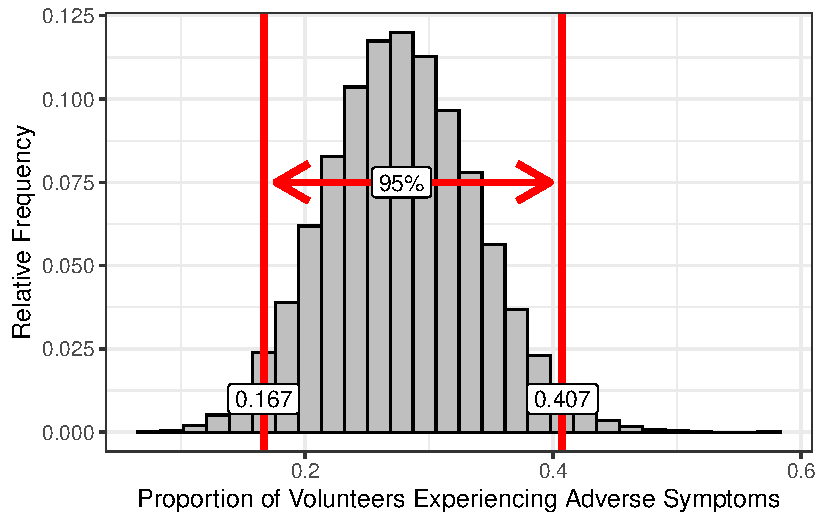
\includegraphics[width=0.8\textwidth,height=\textheight]{./images/fig-samplingdistns-deepwater-ci-1.pdf}

}

\caption{\label{fig-samplingdistns-deepwater-ci}Construction of a
confidence interval via bootstrapping for the proportion of volunteers
assigned to wildlife who develop adverse symptoms based on a sample of
54 volunteers.}

\end{figure}%

\begin{tcolorbox}[enhanced jigsaw, breakable, titlerule=0mm, colframe=quarto-callout-tip-color-frame, bottomtitle=1mm, opacityback=0, rightrule=.15mm, toptitle=1mm, arc=.35mm, bottomrule=.15mm, left=2mm, title=\textcolor{quarto-callout-tip-color}{\faLightbulb}\hspace{0.5em}{Process for Constructing a Confidence Interval}, leftrule=.75mm, coltitle=black, toprule=.15mm, colbacktitle=quarto-callout-tip-color!10!white, colback=white, opacitybacktitle=0.6]

The following is a general procedure for constructing confidence
intervals:

\begin{enumerate}
\def\labelenumi{\arabic{enumi}.}
\tightlist
\item
  Choose a confidence level \(k\) (a decimal between 0 and 1, for
  example 0.95).
\item
  Construct a model for the sampling distribution of the statistic.
\item
  Grab the middle \(100k\)\% of values from the model in step (2).
\end{enumerate}

Notice that the definition of a confidence interval, and this general
procedure, apply regardless of the technique used for constructing the
model of the sampling distribution.

\end{tcolorbox}

Confidence intervals are often misinterpreted; this comes from their
dependence on repeated sampling. When thinking about confidence
intervals, think about playing a game of ring toss: you toss a ring in
hopes of landing on top of a target. The target is the parameter
characterizing the population. The confidence interval is like a ring.
Since the confidence interval is constructed from a model of the
sampling distribution, it changes with each sample; that is, the
confidence interval itself is a statistic. Just like in ring toss where
the ring moves with each toss, the confidence interval moves with each
sample. However, the target (the parameter of interest) stays fixed.
Because of this, there are many incorrect interpretations.

\section{Incorrect Interpretations of a Confidence
Interval}\label{incorrect-interpretations-of-a-confidence-interval}

Suppose we have a \(k\)\% confidence interval; the following are
incorrect interpretations of the interval:

\begin{itemize}
\tightlist
\item
  There is a \(k\)\% chance that individuals in the population have a
  value of the variable within the confidence interval.
\item
  There is a \(k\)\% chance (or we are \(k\)\% sure) that the parameter
  of interest is inside the confidence interval.
\item
  If we were to repeat the study, there is a \(k\)\% chance we would see
  a statistic inside this confidence interval.
\end{itemize}

The first statement above is incorrect because it neglects that a
confidence interval comes from a model for the \emph{sampling
distribution} not the \emph{distribution of the sample}. And, sampling
distributions describe the variability in \emph{statistics}, not the
variability of individuals in the population or sample. Therefore, a
confidence interval cannot make statements about where individual
observations will fall.

The second statement above is incorrect because it treats the parameter
as the thing that is moving. Remember, the target stays fixed in ring
toss; so, we can't say there is a probability the target will move into
the ring. It is tempting to say ``but since the ring is moving, we can
have a chance of catching the target.'' That is a true statement
\emph{before you throw the ring}. However, once the ring is tossed, you
either captured the target or you did not; it no longer makes sense to
say ``I captured the target with 95\% probability.'' The same holds for
confidence intervals. Once the data has been collected, the confidence
interval is a fixed quantity. At this point, neither the estimate nor
the parameter is moving; so, there is no probability left (it either
captured the parameter or it did not). So, the second statement is
really ignoring the dependence of confidence interval interpretations on
repeated sampling.

The third statement above is incorrect because it neglects the idea that
the confidence interval changes with each new sample. Just as the ring
changes location with each toss, so does the confidence interval.

For the Deepwater Horizon Case Study, our 95\% confidence interval was
(0.167, 0.407). Applying the above, the following are \textbf{incorrect}
interpretations:

\begin{itemize}
\tightlist
\item
  There is a 95\% chance that the proportion of volunteers assigned to
  clean wildlife who will experience adverse symptoms is between 0.167
  and 0.407.
\item
  95\% of volunteers assigned to clean wildlife in our sample (or
  population) had a value between 0.167 and 0.407.
\end{itemize}

Returning to how we motivated confidence intervals, appropriate
interpretations rely on the idea of their capturing reasonable values of
the parameter:

\begin{itemize}
\tightlist
\item
  The data is consistent with between 16.7\% and 40.7\% of volunteers
  assigned to clean wildlife experiencing adverse symptoms.
\end{itemize}

We recommend sticking to interpreting a confidence interval as
specifying reasonable values for the parameter.

\begin{tcolorbox}[enhanced jigsaw, breakable, titlerule=0mm, colframe=quarto-callout-tip-color-frame, bottomtitle=1mm, opacityback=0, rightrule=.15mm, toptitle=1mm, arc=.35mm, bottomrule=.15mm, left=2mm, title=\textcolor{quarto-callout-tip-color}{\faLightbulb}\hspace{0.5em}{Big Idea}, leftrule=.75mm, coltitle=black, toprule=.15mm, colbacktitle=quarto-callout-tip-color!10!white, colback=white, opacitybacktitle=0.6]

Confidence intervals specify \emph{reasonable} values of the parameter
based on the data observed.

\end{tcolorbox}

\begin{tcolorbox}[enhanced jigsaw, breakable, titlerule=0mm, colframe=quarto-callout-note-color-frame, bottomtitle=1mm, opacityback=0, rightrule=.15mm, toptitle=1mm, arc=.35mm, bottomrule=.15mm, left=2mm, title=\textcolor{quarto-callout-note-color}{\faInfo}\hspace{0.5em}{Note}, leftrule=.75mm, coltitle=black, toprule=.15mm, colbacktitle=quarto-callout-note-color!10!white, colback=white, opacitybacktitle=0.6]

Other texts will interpret confidence intervals with statements like
``we are 95\% confident that the parameter is inside the interval.'' We
do not recommend this language because the word ``confident'' is
interpreted as ``sure'' in practice, and that leads to an incorrect
interpretation.

\end{tcolorbox}

This is a difficult concept to wrap our heads around; it seems natural
to associate the percentage with the values we have obtained. However,
our confidence is in the \emph{process}, not the resulting interval
itself (Figure~\ref{fig-samplingdistns-ci-process}). That is, 95\%
confidence intervals work 95\% of the time; however, this statement is
about the process of constructing confidence intervals. Once we have
computed a confidence interval, it has either worked or not; the problem
is of course, that since we do not know the parameter, we will never
know if it worked or not. For this reason, we prefer the interpretation
of a confidence interval which avoids these subtleties: a confidence
interval specifies the reasonable values of the parameter. The
percentage (95\% vs 99\% for example) then just specifies what we mean
by ``reasonable.''

\begin{figure}

\centering{

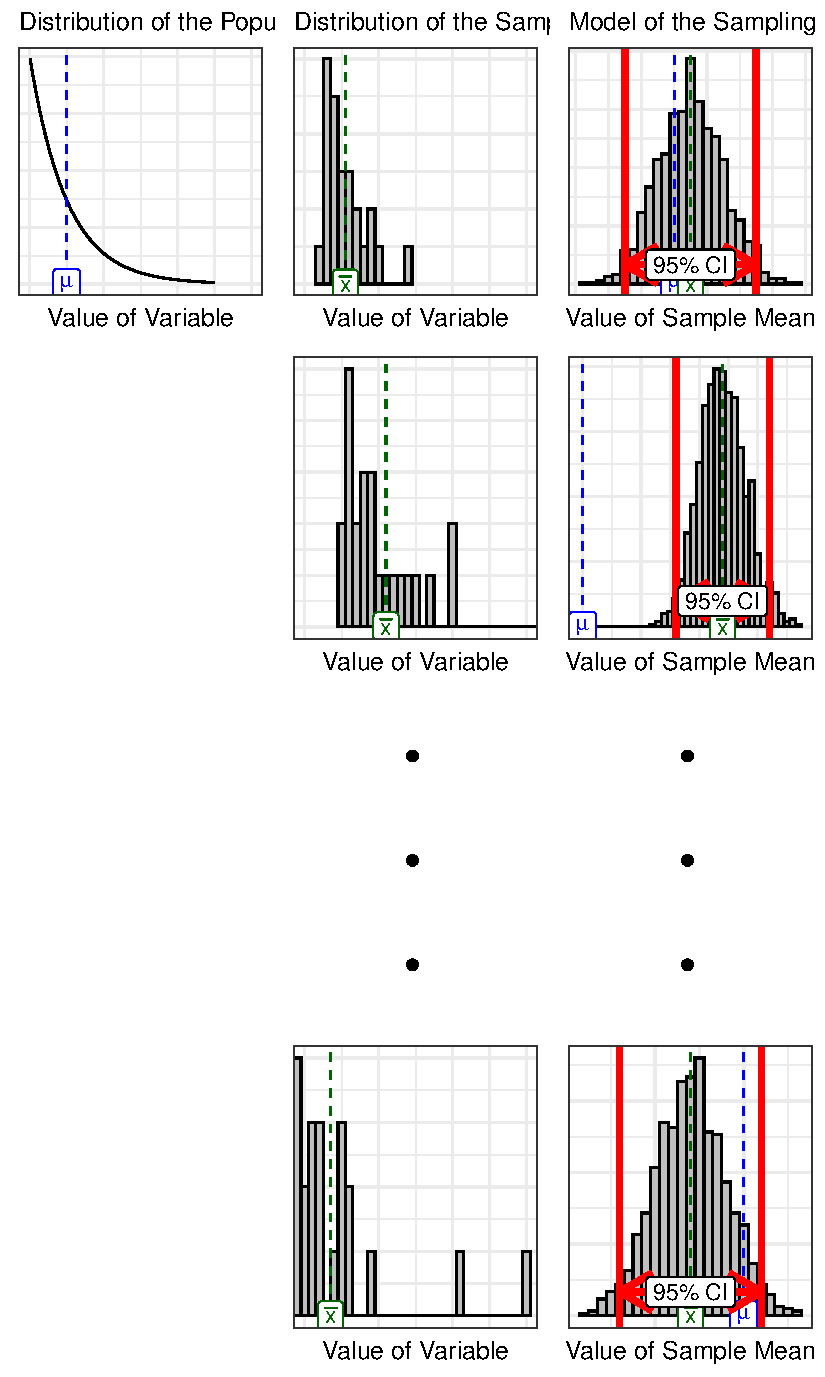
\includegraphics[width=0.8\textwidth,height=\textheight]{./images/fig-samplingdistns-ci-process-1.pdf}

}

\caption{\label{fig-samplingdistns-ci-process}Performance of the
confidence interval process (for the sample mean) across repeated
samples. Our idea of ``confidence'' requires repeated sampling. The
process of constructing a 95\% confidence interval captures the
parameter in 95\% of repeated samples; it is not the specific interval,
but the process that works 95\% of the time.}

\end{figure}%

It may seem like a good idea to make a 100\% confidence interval to be
sure we always capture the parameter. But, such intervals are not
helpful in practice. For example, a 100\% confidence interval for the
proportion of volunteers experiencing adverse symptoms would be (0, 1).
But, this is useless; it essentially says that the proportion has to be
a number between 0 and 1, but we already knew that since all proportions
are between 0 and 1 by definition. Therefore, we must balance the
confidence we desire with the amount of information the interval
conveys.

\begin{tcolorbox}[enhanced jigsaw, breakable, titlerule=0mm, colframe=quarto-callout-tip-color-frame, bottomtitle=1mm, opacityback=0, rightrule=.15mm, toptitle=1mm, arc=.35mm, bottomrule=.15mm, left=2mm, title=\textcolor{quarto-callout-tip-color}{\faLightbulb}\hspace{0.5em}{Big Idea}, leftrule=.75mm, coltitle=black, toprule=.15mm, colbacktitle=quarto-callout-tip-color!10!white, colback=white, opacitybacktitle=0.6]

If you want both a high level of confidence but also a narrow interval,
increase the sample size. As the sample size increases, the variability
in the statistic decreases leading to a narrower interval.

\end{tcolorbox}

\begin{tcolorbox}[enhanced jigsaw, breakable, titlerule=0mm, colframe=quarto-callout-note-color-frame, bottomtitle=1mm, opacityback=0, rightrule=.15mm, toptitle=1mm, arc=.35mm, bottomrule=.15mm, left=2mm, title=\textcolor{quarto-callout-note-color}{\faInfo}\hspace{0.5em}{Note}, leftrule=.75mm, coltitle=black, toprule=.15mm, colbacktitle=quarto-callout-note-color!10!white, colback=white, opacitybacktitle=0.6]

95\% confidence intervals are the most common in practice; however,
90\%, 98\%, and 99\% intervals are also used. It is extremely rare to
use less than a 90\% confidence interval.

\end{tcolorbox}

\section{Bringing it All Together}\label{bringing-it-all-together}

Consider the following question:

\begin{quote}
Does the study provide evidence that more than 1 in 5 volunteers
assigned to clean wildlife develop adverse respiratory symptoms?
\end{quote}

Let's answer this question using a confidence interval. Based on the
data obtained, we found that the 95\% confidence interval (CI) for the
proportion of volunteers experiencing adverse symptoms to be (0.167,
0.407). Is this data consistent with more than 1 in 5 volunteers
developing adverse symptoms? Yes, since there are proportions within
this interval which are larger than 0.2. But, \emph{consistency} is not
the same as \emph{evidence}; remember, evidence is the idea of ``beyond
a reasonable doubt.'' After all, is this data \emph{consistent} with
less than 1 in 5 volunteers developing adverse symptoms? Yes, since
there are proportions within this interval which are less than 0.2.

Confidence intervals specify reasonable values --- those values of the
parameter which are consistent with the data. This data is then
consistent with proportions that are both less than 0.2 and greater than
0.2. So, what can we say then? We can say that the study does \emph{not
provide evidence} that more than 1 in 5 volunteers assigned to clean
wildlife develop adverse respiratory symptoms, but the data \emph{is
consistent} with this claim.

We can say that the study \emph{provides evidence} the proportion of
volunteers who develop symptoms is less than 0.5; the study provides
evidence the proportion of volunteers who develop symptoms is larger
than 0.1. That is, the study provides evidence that more than 10\% of
volunteers develop adverse symptoms and provides evidence this
percentage is not larger than 50\%. How do we know? Because values less
than 10\% are not reasonable values of the parameter based on the 95\%
confidence interval. Values like 0.1 are outside of the confidence
interval and are therefore not reasonable. Similarly, values above 0.5
are outside the confidence interval and are therefore not reasonable.

The power of a model for the sampling distribution is that it allows us
to determine which values of a parameter are reasonable and which values
are not.

\chapter{Quantifying the Evidence (Rejecting Bad
Models)}\label{sec-nulldistns}

Again, the goal of statistical inference is to use the sample as a
snapshot of the underlying population
(Figure~\ref{fig-basics-statistical-process}). Recall that there are
essentially two categories of questions we ask when trying to perform
inference:

\begin{itemize}
\tightlist
\item
  Estimation: for example, what \emph{proportion} of volunteers who
  clean wildlife following an oil spill experience adverse respiratory
  symptoms?
\item
  Hypothesis Testing: is it reasonable no more than 1 in 5 volunteers
  who clean wildlife following an oil spill will experience adverse
  respiratory symptoms; or, is there evidence more than 1 in 5
  volunteers who clean wildlife following an oil spill will experience
  adverse respiratory symptoms?
\end{itemize}

In Chapter~\ref{sec-samplingdistns}, we addressed these questions
through the use of confidence intervals --- by specifying reasonable
values of the parameters through a model of the sampling distribution.
However, when our goal is testing a specific hypothesis, there is a
second approach; this latter approach is useful when the research
question involves multiple parameters and creating a confidence interval
is challenging (see Unit III).

In Chapter~\ref{sec-questions}, we described hypothesis testing as being
similar to performing a trial in a course of law. Once the prosecution
and defense have each presented their case, the jury deliberates and
makes one of two decisions:

\begin{enumerate}
\def\labelenumi{\arabic{enumi}.}
\tightlist
\item
  Vote ``guilty.'' This happens when the jury believes the facts of the
  case are not consistent with an innocent defendant; therefore, the
  prosecution has convinced the jury (``beyond reasonable doubt'') that
  their initial assumption of innocence is not warranted.
\item
  Vote ``not guilty.'' This happens when the jury believes the facts of
  the case are consistent with an innocent defendant; that is, while the
  prosecution presented a case that may have been consistent with a
  guilty defendant, it is still ``reasonable'' that the defendant is
  innocent. That is, the prosecution has not convinced the jury that
  their initial assumption of innocence is unwarranted.
\end{enumerate}

Similar to a jury, we have a working hypothesis (the null hypothesis);
we must quantify the evidence from the sample against this hypothesis.
If we are convinced that the data is not consistent with this working
hypothesis, we will declare we have evidence for the alternative
hypothesis. Our goal in this section is to quantify that evidence.

\section{Some Subtleties}\label{some-subtleties}

We have described hypothesis testing as being similar to a U.S. trial.
That analogy is also helpful in pointing out some subtleties in how we
interpret our results. We take a moment to discuss those subtleties
before discussing the process itself in order to avoid erroneous
interpretations.

The jury weighs the case \emph{under the assumption of innocence}. That
is, they first develop a working hypothesis (the defendant is innocent).
Then, the likelihood of the case against the defendant \emph{under this
assumption} is determined. For example, if a defendant were innocent of
murder, it is unlikely to have five eye witnesses stating the defendant
was seen standing over the victim, holding the murder weapon, and
screaming ``I killed him!'' Since that case against the defendant does
not jive with innocence, the jury convicts. If, however, the only case
presented is that five eye witnesses place the defendant in the same
city as the victim and the defendant matches the description of someone
seen fleeing the crime scene, then the jury would not convict. Why?
Because the case presented, while pointing toward guilt, is not
overwhelming; these things could have happened by chance alone.
Therefore, the case, while \emph{consistent} with guilt does not provide
\emph{evidence} for guilt.

As in Chapter~\ref{sec-samplingdistns}, we are making a distinction
between ``evidence for'' a hypothesis and the data being ``consistent
with'' a hypothesis. Evidence for a particular claim is only established
by providing evidence against the opposite statement. However,
consistency can be established without disqualifying any other
statement; that is, data can be consistent with two opposing claims, but
data cannot provide evidence for two opposing claims.

\begin{tcolorbox}[enhanced jigsaw, breakable, titlerule=0mm, colframe=quarto-callout-tip-color-frame, bottomtitle=1mm, opacityback=0, rightrule=.15mm, toptitle=1mm, arc=.35mm, bottomrule=.15mm, left=2mm, title=\textcolor{quarto-callout-tip-color}{\faLightbulb}\hspace{0.5em}{Big Idea}, leftrule=.75mm, coltitle=black, toprule=.15mm, colbacktitle=quarto-callout-tip-color!10!white, colback=white, opacitybacktitle=0.6]

Data can be \emph{consistent} with two opposing claims, but data cannot
provide \emph{evidence} for two opposing claims.

\end{tcolorbox}

Also notice that a jury saying ``not guilty'' is not the same as saying
``innocent.'' That is, a lack of evidence to convict does not imply the
defendant is innocent. A lack of evidence is simply a lack of evidence.
The defendant may still be guilty, but the evidence has just not proven
it.

\begin{tcolorbox}[enhanced jigsaw, breakable, titlerule=0mm, colframe=quarto-callout-tip-color-frame, bottomtitle=1mm, opacityback=0, rightrule=.15mm, toptitle=1mm, arc=.35mm, bottomrule=.15mm, left=2mm, title=\textcolor{quarto-callout-tip-color}{\faLightbulb}\hspace{0.5em}{Big Idea}, leftrule=.75mm, coltitle=black, toprule=.15mm, colbacktitle=quarto-callout-tip-color!10!white, colback=white, opacitybacktitle=0.6]

A lack of evidence for a signal is not evidence for a lack of a signal.

\end{tcolorbox}

Similarly, when performing a hypothesis test, we will weigh the data
\emph{under the null hypothesis} (our working assumption). Then, the
likelihood of our data occurring by chance alone \emph{under this
hypothesis} is determined. If that likelihood is small (data is not
consistent with the null hypothesis), we can conclude the data supports
the alternative hypothesis (guilty). If, however, that likelihood is
large (data is consistent with the null hypothesis), we can only
conclude that the data is consistent with the hypotheses. We are
\emph{not} able to say ``supports the null'' because that would be like
saying a defendant is innocent. We can't prove innocence because we
started by assuming it!

\section{Assuming the Null
Hypothesis}\label{assuming-the-null-hypothesis}

Consider the question we have been asking regarding the Deepwater
Horizon Case Study discussed in Chapter~\ref{sec-caseDeepwater}:

\begin{quote}
Is there evidence that more than 1 in 5 volunteers assigned to clean
wildlife develop adverse respiratory conditions?
\end{quote}

Remember, we framed this question through statements about a parameter
in Chapter~\ref{sec-questions}:

\begin{quote}
\(H_0:\) the proportion of volunteers assigned to clean wildlife that
develop adverse respiratory symptoms is no more than 0.20.\\
\(H_1:\) the proportion of volunteers assigned to clean wildlife that
develop adverse respiratory symptoms exceeds 0.20.
\end{quote}

Within the sample we observed that 27.8\% of volunteers experienced
adverse symptoms, which is certainly more than the 0.20; drawing the
connection to the courtroom, the 27.8\% is the case presented by the
prosecution. From this, we see that the data is at least trending toward
the alternative hypothesis. Just as a jury has to ask whether the case
is overwhelming (no longer consistent with an innocent defendant) or
whether the case is consistent with an innocent defendant, we must ask
whether the 27.8\% is overwhelming (no longer consistent with 1 in 5
volunteers developing adverse respiratory conditions) or consistent with
the null hypothesis. After all, it is possible that we just have a
strange sample; that is, it is possible our data is a fluke, resulting
in an estimate larger than 0.2 by chance alone.

As we discussed in the previous chapter, we expect our estimate to vary
to some degree from one sample to another. Essentially, we need to know
if 27.8\% of volunteers experiencing symptoms is a strong signal that
the rate within the population is larger than 0.2 (1 in 5) or whether
27.8\% is simply a fluke that might happen due to sampling variability.
While we are going to be attacking the question differently in this
chapter than the previous, we see that the key is still variability in
the estimate. That is, we are back to the \emph{Fourth Fundamental Idea
of Inference}. As stated above, in order to determine evidence for one
statement (captured by the alternative hypothesis), we begin by assuming
the opposite statement (captured by the null hypothesis) as our working
assumption. That is, if we want to know if 27.8\% of volunteers
experiencing adverse symptoms is ``evidence,'' we need to figure out
what we \emph{expect} to happen \emph{if only 1 in 5 volunteers actually
develop adverse respiratory symptoms} (the statement represented by the
equality portion of the null hypothesis).

Consider this last statement. It is equivalent to saying ``what type of
actions would we expect of an innocent person?'' Only when we know what
to expect can we determine if the case in front of us is extreme enough
to convict. Only when we know what to expect can we determine if the
observed sample provides \emph{evidence} in favor of the alternative.
Our strategy is to enter a fake world\ldots a world in which exactly 1
in 5 volunteers actually develop respiratory symptoms. That is, we enter
a world in which the null hypothesis is true. Now, in this world, how do
we know what to expect? We construct the sampling distribution for the
proportion under this assumption that the null hypothesis is true; this
is known as the \textbf{null distribution}.

\begin{definition}[Null
Distribution]\protect\hypertarget{def-null-distribution}{}\label{def-null-distribution}

The sampling distribution of a statistic \emph{when} the null hypothesis
is true.

\end{definition}

The null distribution, the last in our \emph{Distributional Quartet}, is
a sampling distribution; it is just a sampling distribution for a world
in which the null hypothesis is true. As a result, the process for
constructing the null distribution is very similar to the process for
constructing the sampling distribution (illustrated in
Figure~\ref{fig-nulldistns-null-distribution}):

\begin{enumerate}
\def\labelenumi{\arabic{enumi}.}
\tightlist
\item
  Sample randomly from a fake population where the null hypothesis is
  true.
\item
  For each sample, compute the statistic of interest.
\item
  Repeat steps 1 and 2 several thousand times.
\item
  Plot the statistics retained from each sample.
\end{enumerate}

\begin{figure}

\centering{

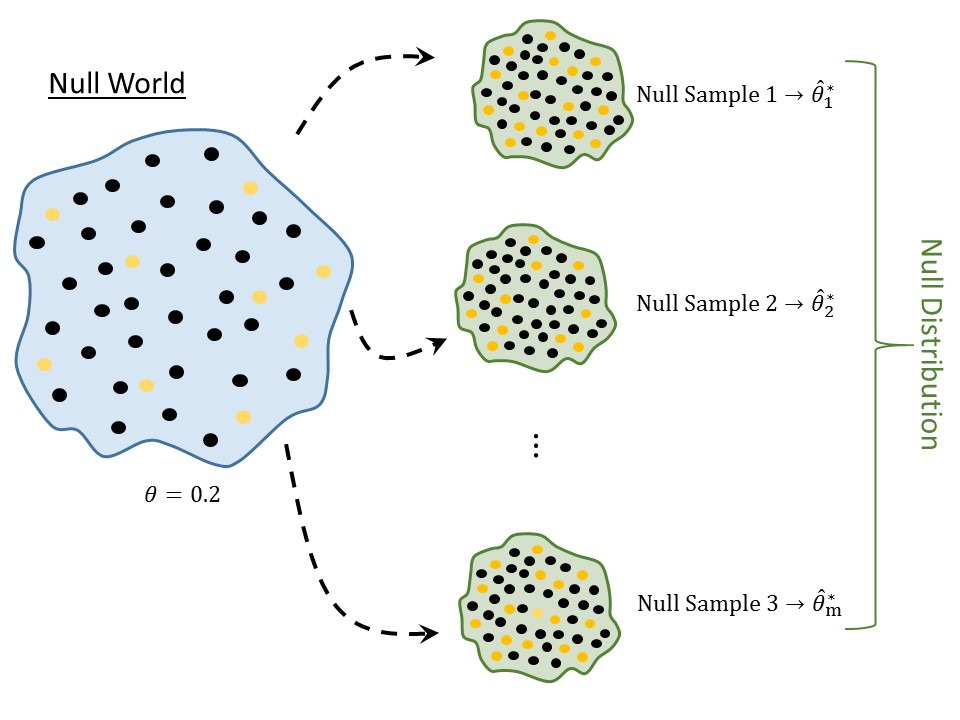
\includegraphics[width=0.8\textwidth,height=\textheight]{./images/NullDistns-Null-Distribution.jpg}

}

\caption{\label{fig-nulldistns-null-distribution}Illustration of
constructing a null distribution. Notice the similarity to constructing
the sampling distributon.}

\end{figure}%

Notice that these are the same steps as constructing a sampling
distribution with the exception that instead of sampling from the
population of interest, we sample from a hypothetical population in
which the null distribution is true.

Since the null distribution is a sampling distribution when a particular
hypothesis is true, we are constrained by the same limitations as
before. Namely, we are generally unable to construct the actual the null
distribution; instead, we must construct a model for it. More, since the
null distribution is a sampling distribution, the same techniques we use
for modeling the sampling distribution can be modified to model the null
distribution. The key is to enforce the null hypothesis to be true. As
with sampling distributions, we emphasize the empirical model approach.

Using the computer, we first create a virtual world in which the null
hypothesis is true. This often involves adjusting the original sample in
order to make it consistent with having been drawn from a population in
which the null hypothesis were true. The augmented data becomes the null
world. We are then able to bootstrap from the augmented data to simulate
repeated sampling when the null hypothesis is true. The details of this
procedure are beyond the scope of our current discussion; it is more
important to understand the conceptual idea of a null distribution at
this point.

Figure~\ref{fig-nulldistns-deepwater-null} represents a model for the
null distribution of the proportion of volunteers in a sample of 54
assigned to clean wildlife which would develop adverse symptoms when the
we assume the actual proportion is 0.20.

\begin{tcolorbox}[enhanced jigsaw, breakable, titlerule=0mm, colframe=quarto-callout-note-color-frame, bottomtitle=1mm, opacityback=0, rightrule=.15mm, toptitle=1mm, arc=.35mm, bottomrule=.15mm, left=2mm, title=\textcolor{quarto-callout-note-color}{\faInfo}\hspace{0.5em}{Note}, leftrule=.75mm, coltitle=black, toprule=.15mm, colbacktitle=quarto-callout-note-color!10!white, colback=white, opacitybacktitle=0.6]

A null distribution is tied to a specific null hypothesis. A sampling
distribution does not require a hypothesis to construct. So, while a
sampling distribution could be used to address a variety of null
hypotheses, a null distribution can only be used to address the
corresponding set of hypotheses for which it was developed.

\end{tcolorbox}

\begin{figure}

\centering{

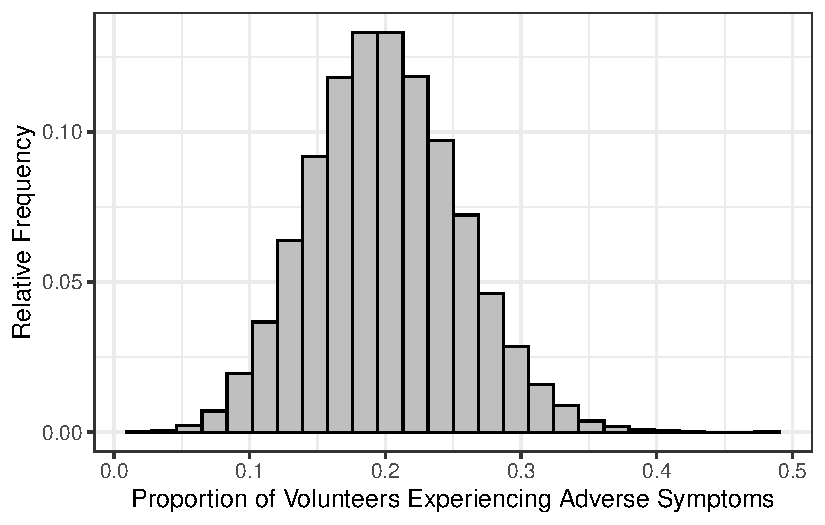
\includegraphics[width=0.8\textwidth,height=\textheight]{./images/fig-nulldistns-deepwater-null-1.pdf}

}

\caption{\label{fig-nulldistns-deepwater-null}Null distribution for the
proportion of volunteers assigned to clean wildlife experiencing adverse
respiratory symptoms. The null hypothesis is that the proportion is
0.20; this model is based on a sample size of 54.}

\end{figure}%

As we are introducing the concept of a null distribution, we will stick
to modeling the null distribution of a statistic. Often times in a
statistical analysis, the null distribution is computed for a numerical
quantity known as a standardized statistic (see
Chapter~\ref{sec-teststat}).

\section{Using the Null Distribution}\label{using-the-null-distribution}

From Figure~\ref{fig-nulldistns-deepwater-null}, we see that \emph{if
the null hypothesis were true} --- if only 1 in 5 volunteers assigned to
clean wildlife experienced symptoms --- then in a sample of 54
individuals, we would expect the proportion who experienced symptoms to
be somewhere between 0.1 and 0.3. So, we can think of the null
distribution as setting up our expectations of what we should have
observed \emph{if the null hypothesis were true}. For example, \emph{if
the null hypothesis were true}, it would be nearly impossible that half
of the individuals experienced symptoms. We are able to say that since
0.5 is way off in the tail region of the distribution, and we know that
values in the tail region are more extreme. The question is then how
extreme is \emph{our} sample? Again, the null distribution is just
setting up expectations; to determine if our sample provides evidence
against the null hypothesis, we have to weigh the data against those
expectations.

In our sample, we observed 27.8\% of volunteers experience symptoms.
Since 0.278 is towards the center of the distribution, we would say that
it is not an extreme sample. In order to quantify how extreme (or not
extreme) it is, we compute the fraction of values which are more extreme
(larger in this case) than the value observed; that is, we compute the
fraction of values that appear further to the right than 0.278 in the
null distribution. Figure~\ref{fig-nulldistns-deepwater-pvalue}
illustrates this computation. Based on the null distribution, there is a
10.6\% chance that \emph{if the null hypothesis were true} --- only 1 in
5 volunteers actually experienced symptoms --- that in a random sample
of 54 volunteers we would obtain data this extreme or more so (an
observed proportion of 0.278 or larger) by chance alone (due to sampling
variability). This area is known as the \textbf{p-value}.

Essentially, this tail area is quantifying the strength of the evidence.
The smaller this area, the further in the tail region our observed
statistic is; that is, the smaller this area, the more unexpected our
data. Therefore, small areas indicate that the data (our case) does not
jive with our expectations under the null hypothesis (innocence),
forcing us to conclude the data provides \emph{evidence against} the
null hypothesis (guilty verdict). On the other hand, the larger this
area, the closer toward the center our observed statistic is; that is,
the larger this area, the less unexpected our data. Therefore, large
areas indicate that the data (our case) is consistent with our
expectations under the null hypothesis (innocence), forcing us to
conclude the data is \emph{consistent with} the null hypothesis (not
guilty verdict).

\begin{definition}[P-Value]\protect\hypertarget{def-pvalue}{}\label{def-pvalue}

The probability, assuming the null hypothesis is true, that we would
observe a statistic, from sampling variability alone, as extreme or more
so as that observed in our sample. The p-value quantifies the strength
of evidence against the null hypothesis, with smaller values indicating
stronger evidence.

\end{definition}

For the Deepwater Horizon Case Study, we observed 27.8\%, which is
towards the center of the null distribution, and our p-value is quite
large. Therefore, our data is consistent with what we might expect if
the null hypothesis were true, and we conclude that there is no evidence
that the rate of those experiencing symptoms exceeds 1 in 5.

\begin{figure}

\centering{

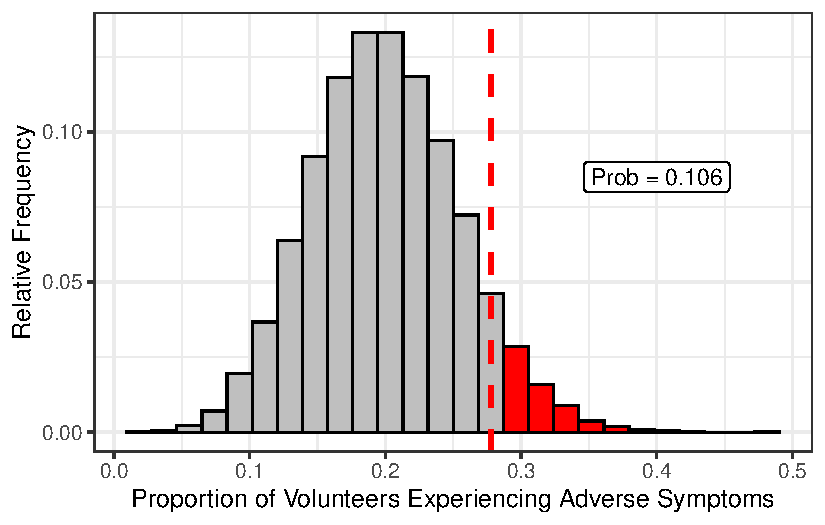
\includegraphics[width=0.8\textwidth,height=\textheight]{./images/fig-nulldistns-deepwater-pvalue-1.pdf}

}

\caption{\label{fig-nulldistns-deepwater-pvalue}Likelihood of obtaining
a statistic as extreme or moreso as that of the original sample when the
parameter of interest is the proportion of volunteers assigned to clean
wildlife experiencing adverse respiratory symptoms. The null hypothesis
is that the proportion is 0.20; this is based on a sample of size 54.}

\end{figure}%

It is natural to ask ``how small does the p-value need to be to prove a
statement?'' Like a trial, the strength of the case presented depends on
the context. In some studies, a p-value less than 0.01 may be strong
evidence while in other studies a p-value less than \(10^{-6}\) is
required. And, as in a trial, it is not only the strength of the case
but the type of information presented (the presence of DNA may carry
more weight than the presence of fingerprints). In statistics, it is
important to consider the \emph{effect size} (some measure of the signal
in the data) as well as the p-value. That is, consider whether the
difference between the estimate and the null value is actually large for
the specific context; this is always based on subject-matter expertise.
It is often helpful, whenever possible, to report a confidence interval
alongside a p-value.

\begin{tcolorbox}[enhanced jigsaw, breakable, titlerule=0mm, colframe=quarto-callout-tip-color-frame, bottomtitle=1mm, opacityback=0, rightrule=.15mm, toptitle=1mm, arc=.35mm, bottomrule=.15mm, left=2mm, title=\textcolor{quarto-callout-tip-color}{\faLightbulb}\hspace{0.5em}{Gradient of Evidence}, leftrule=.75mm, coltitle=black, toprule=.15mm, colbacktitle=quarto-callout-tip-color!10!white, colback=white, opacitybacktitle=0.6]

While what constitutes evidence may vary from discipline to discipline,
the list below is a good rule of thumb:

\begin{itemize}
\tightlist
\item
  \(p \geq 0.1\): no evidence against the null hypothesis.
\item
  \(0.05 \leq p < 0.1\): weak evidence against the null hypothesis.
\item
  \(0.01 \leq p < 0.05\): some evidence against the null hypothesis.
\item
  \(0.001 \leq p < 0.01\): evidence against the null hypothesis.
\item
  \(p < 0.001\): strong evidence against the null hypothesis.
\end{itemize}

Of course, evidence ``against the null hypothesis'' is equivalent to
evidence ``for the alternative hypothesis.'' As with any rule of thumb,
the above gradient should not be considered binding and may vary
depending on the application.

\end{tcolorbox}

We can think of the p-value as a measure of whether the data is able to
\emph{discern} the difference between a hypothesized value (the null
value) and that observed in the sample. When the p-value is sufficiently
low, we might say there is a ``statistically discernible'' difference.

\begin{tcolorbox}[enhanced jigsaw, breakable, titlerule=0mm, colframe=quarto-callout-warning-color-frame, bottomtitle=1mm, opacityback=0, rightrule=.15mm, toptitle=1mm, arc=.35mm, bottomrule=.15mm, left=2mm, title=\textcolor{quarto-callout-warning-color}{\faExclamationTriangle}\hspace{0.5em}{Warning}, leftrule=.75mm, coltitle=black, toprule=.15mm, colbacktitle=quarto-callout-warning-color!10!white, colback=white, opacitybacktitle=0.6]

You may see some authors refer to a ``significance level,'' often
denoted by the Greek letter alpha. The significance level is a
pre-determined threshold for declaring a p-value to be ``small.'' That
is, p-values below the significance level indicate there is evidence
against the null hypothesis, and p-values above the significance level
indicate there is no evidence against the null hypothesis.

This has led to authors stating that a study shows a ``statistically
\emph{significant}'' difference. We dislike this language because the
term ``significant'' suggests the difference is important. However, we
may be able to detect a difference that is not meaningful in real life.
Determining importance is a matter for discipline experts.

We prefer the term ``statistically discernible'' and the gradient of
evidence provided above instead of the binary decision that results from
defining a significance level.

\end{tcolorbox}

As Regina Nuzzo once quipped\footnote{Stated in a keynote presentation
  at USCOTS23
  (\url{https://www.causeweb.org/cause/uscots/uscots23/keynotes/1}).},
we can think of the p-value as an ``index of holy shitness.''
Essentially, small p-values tell you the data was really unexpected
under the null hypothesis (``wow, that was unexpected''); and, larger
p-values tell you the data was about what you would expect under the
null hypothesis (``yeah, that was about what we expected''). When your
data surprises you (from the perspective of the null hypothesis), then
we start to believe that our underlying assumption about that data (the
null hypothesis) is not appropriate.

\begin{tcolorbox}[enhanced jigsaw, breakable, titlerule=0mm, colframe=quarto-callout-tip-color-frame, bottomtitle=1mm, opacityback=0, rightrule=.15mm, toptitle=1mm, arc=.35mm, bottomrule=.15mm, left=2mm, title=\textcolor{quarto-callout-tip-color}{\faLightbulb}\hspace{0.5em}{Big Idea}, leftrule=.75mm, coltitle=black, toprule=.15mm, colbacktitle=quarto-callout-tip-color!10!white, colback=white, opacitybacktitle=0.6]

A p-value should never be reported in isolation. It should always be
accompanied by a confidence interval, a numerical summary of the data,
or a graphical summary of the data --- something which indicates the
effect size and variability in the data.

\end{tcolorbox}

\begin{tcolorbox}[enhanced jigsaw, breakable, titlerule=0mm, colframe=quarto-callout-note-color-frame, bottomtitle=1mm, opacityback=0, rightrule=.15mm, toptitle=1mm, arc=.35mm, bottomrule=.15mm, left=2mm, title=\textcolor{quarto-callout-note-color}{\faInfo}\hspace{0.5em}{Note}, leftrule=.75mm, coltitle=black, toprule=.15mm, colbacktitle=quarto-callout-note-color!10!white, colback=white, opacitybacktitle=0.6]

Here, we refer to the ``effect size'' as the impact of the signal in the
data. However, some disciplines rely on standardized effect sizes which
are unit-less measurements. These measurements are typically a ratio of
the difference between the observed statistic and the null value to a
measure of the variability in the data.

Regardless of whether you use the raw effect size or a standardized
effect size, the idea is the same --- you should understand whether the
signal you are detecting in the data is of practical relevance in your
discipline.

\end{tcolorbox}

\begin{tcolorbox}[enhanced jigsaw, breakable, titlerule=0mm, colframe=quarto-callout-tip-color-frame, bottomtitle=1mm, opacityback=0, rightrule=.15mm, toptitle=1mm, arc=.35mm, bottomrule=.15mm, left=2mm, title=\textcolor{quarto-callout-tip-color}{\faLightbulb}\hspace{0.5em}{Process for Computing a P-Value}, leftrule=.75mm, coltitle=black, toprule=.15mm, colbacktitle=quarto-callout-tip-color!10!white, colback=white, opacitybacktitle=0.6]

The following is a general procedure for computing a p-value:

\begin{enumerate}
\def\labelenumi{\arabic{enumi}.}
\tightlist
\item
  Define the null and alternative hypotheses.
\item
  Construct a model for the null distribution of the desired statistic.
\item
  Compute the desired statistic for the original sample.
\item
  Overlay the statistic from step (3) on the model developed in step
  (2), and then compute the area under the curve for values \emph{more
  extreme} than that observed in step (3).
\end{enumerate}

Notice that the definition of a p-value, and this general procedure,
apply regardless of the technique used for constructing the model of the
null distribution.

\end{tcolorbox}

Like confidence intervals, p-values are often misinterpreted. In fact,
they have become so abused that some researchers argue against their
use. It is our opinion that the p-value can be a useful tool once it is
appropriately understood; so, let's dispel some of the misconceptions.

\section{Incorrect Interpretations of a
P-Value}\label{incorrect-interpretations-of-a-p-value}

Suppose we have a p-value of \(p\). The following are incorrect
interpretations of that p-value:

\begin{itemize}
\tightlist
\item
  There is a \(100p\)\% chance that the null hypothesis is correct.
\item
  When \(p\) is large, we have evidence (or ``the data supports'') the
  null hypothesis is correct.
\end{itemize}

The first statement is incorrect because it assumes the parameter is
moving. Hypotheses are statements about parameters, and parameters are
fixed, unknown values. One of the hypotheses is true, and the other is
not. Our ignorance does not change this. Since the parameter is a fixed
value, it does not make sense to think about the likelihood that either
hypothesis is correct. Instead, the p-value quantifies the likelihood of
observing a particular \emph{statistic} assuming the null is true.

The second statement has circular logic. Again, when computing the
p-value, we assumed the null hypothesis was correct; so, we cannot prove
what we start off assuming. It mistakenly assumes that a lack of
evidence for the alternative hypothesis is evidence for the null
hypothesis, but that is not true. A large p-value simply indicates the
data is consistent with the null hypothesis, but a large p-value cannot
provide evidence to support the null hypothesis. This is similar to the
fact that in a trial, the jury can declare ``not guilty'' (you did not
convince us of guilt), but they do not declare ``innocent.''

For the Deepwater Horizon Case Study, we obtained a p-value of 0.106.
Considering the above, the following are \textbf{incorrect}
interpretations:

\begin{itemize}
\tightlist
\item
  There is a 10.6\% chance that only 1 in 5 volunteers assigned to clean
  wildlife will experience adverse symptoms.
\item
  Since the p-value is large, there is evidence (or the data supports
  the claim) that 1 in 5 volunteers assigned to clean wildlife will
  experience adverse symptoms.
\end{itemize}

Thinking about the p-value correctly, we are led to the following
conclusion:

\begin{itemize}
\tightlist
\item
  With a p-value of 0.106, our data is \emph{consistent with} only 1 in
  5 volunteers assigned to clean wildlife experiencing adverse
  respiratory symptoms.
\end{itemize}

Unfortunately, our data is also \emph{consistent with} more than 1 in 5
volunteers assigned to clean wildlife experiencing adverse respiratory
symptoms. The fact that our data is consistent with both hypotheses may
be an unsatisfying conclusion, but it is still a conclusion nonetheless.

This process of using a p-value to quantify the evidence against a
particular model is captured in our last of the \emph{Five Fundamental
Ideas of Inference}.

\begin{tcolorbox}[enhanced jigsaw, breakable, titlerule=0mm, colframe=quarto-callout-important-color-frame, bottomtitle=1mm, opacityback=0, rightrule=.15mm, toptitle=1mm, arc=.35mm, bottomrule=.15mm, left=2mm, title=\textcolor{quarto-callout-important-color}{\faExclamation}\hspace{0.5em}{Fundamental Idea V}, leftrule=.75mm, coltitle=black, toprule=.15mm, colbacktitle=quarto-callout-important-color!10!white, colback=white, opacitybacktitle=0.6]

With a model for the distribution of a statistic under a proposed model,
we can quantify the the likelihood of an observed sample under that
proposed model. This allows us to draw conclusions about the
corresponding parameter, and therefore the population, of interest.

\end{tcolorbox}

\section{Sampling Distributions vs.~Null
Distributions}\label{sampling-distributions-vs.-null-distributions}

Clearly the sampling distribution and null distribution of a statistic
are closely related. The difference is that the null distribution is
created under a proposed model while the sampling distribution lets the
data speak for itself. It is worth taking just a moment to highlight the
differences in the use of these two components of the
\emph{Distributional Quartet}.

The sampling distribution is centered on the true value of the
parameter; the null distribution is centered on the null value. Once we
assume the null hypothesis is true, we have a value for the parameter;
as a result, we expect the sampling distribution under this assumption
(that is, the null distribution) to be centered on this hypothesized
value. So, null distributions of a statistic are \emph{always} centered
on the null value.

When we model the sampling distribution, this leads to a confidence
interval. That confidence interval specifies the reasonable value of the
parameter based on the observed data.

When we model the null distribution, we are able to compute a p-value.
The p-value quantifies how likely our observed statistic is under the
proposed null hypothesis.

\begin{tcolorbox}[enhanced jigsaw, breakable, titlerule=0mm, colframe=quarto-callout-tip-color-frame, bottomtitle=1mm, opacityback=0, rightrule=.15mm, toptitle=1mm, arc=.35mm, bottomrule=.15mm, left=2mm, title=\textcolor{quarto-callout-tip-color}{\faLightbulb}\hspace{0.5em}{Big Idea}, leftrule=.75mm, coltitle=black, toprule=.15mm, colbacktitle=quarto-callout-tip-color!10!white, colback=white, opacitybacktitle=0.6]

Model the sampling distribution to construct a confidence interval; to
assess a hypothesis the null value is overlaid on the model for the
sampling distribution. Extreme values of the model for the sampling
distribution are unreasonable values for the parameter.

Model the null distribution to compute a p-value; to assess a
hypothesis, the statistic from the sample is overlaid on the model for
the null distribution. Extreme values of the model for the distribution
are values which provide evidence against the null hypothesis.

\end{tcolorbox}

\chapter{Using the Tools Together}\label{sec-recaplanguage}

In this unit, we have introduced the key components in both the language
and logic of statistical inference. In fact, with a firm grasp of the
concepts in this unit, you should be able to read and interpret key
statistical findings. All statistical analyses make use of the
\emph{Five Fundamental Ideas of Inference} and alternate between the
components of the \emph{Distributional Quartet}. The context of each
problem differs, but the logic remains the same. In this chapter, we
present another analysis based on the Deepwater Horizon Case Study of
Chapter~\ref{sec-caseDeepwater}, annotating it along the way to see how
these elements work together fluidly to reach a conclusion.
Specifically, we are interested in the following question:

\begin{quote}
Are volunteers assigned to clean wildlife at higher risk of developing
adverse respiratory symptoms compared to those volunteers who do not
come into direct contact with oil? If so, estimate the increased risk.
\end{quote}

\section{Framing the Question (Fundamental Idea
I)}\label{framing-the-question-fundamental-idea-i}

We are really interested in whether the rate of respiratory symptoms in
one group of volunteers is larger than that in a second group.
Therefore, our working assumption is that the rate of respiratory
symptoms for those assigned to clean wildlife is no more than that for
those assigned to tasks which do not involve direct exposure to oil.
That is, we have

\begin{quote}
\(H_0:\) the rate of adverse respiratory symptoms for volunteers
assigned to clean wildlife is no greater than that for those assigned to
tasks which do not involve direct exposure to oil.\\
\(H_1:\) the rate of adverse respiratory symptoms is greater for
volunteers assigned to clean wildlife compared to those assigned to
tasks which do not involve direct exposure to oil.
\end{quote}

We can also state this more formally with mathematical notation as
follows:

\begin{quote}
Let \(\theta_1\) be the rate of developing adverse respiratory symptoms
for volunteers assigned to clean wildlife.\\
Let \(\theta_2\) be the rate of developing adverse respiratory symptoms
for volunteers assigned to tasks without direct exposure to oil.\\
\(H_0: \theta_1/\theta_2 \leq 1\)\\
\(H_1: \theta_1/\theta_2 > 1\)
\end{quote}

The ratio \(\theta_1/\theta_2\) is known as the \emph{relative risk} as
it captures the increased risk for one group compared to another.

Notice that this is a well-posed question as it centers on parameters
which characterize the population. Therefore, it can be answered with
appropriate data.

\begin{quote}
Distribution of the Population: Our questions of interest are about the
population and therefore focus on characterizing this distribution.
\end{quote}

\section{Getting Good Data (Fundamental Idea
II)}\label{getting-good-data-fundamental-idea-ii}

As we are working with previously collected data, we are unable to
design a good sampling scheme. The only thing we can do at this point is
critique the sample we have. The key question to ask ourselves is
whether there is any reason that this group of volunteers differs
systematically from other volunteers working oil spills. For example,
this oil spill occurred in the Gulf of Mexico; the majority of
volunteers were then naturally residents of Gulf states. It is possible
that these residents are somehow fundamentally different with respect to
their risk of developing adverse respiratory symptoms compared to the
remainder of the United States. If that is the case, the results of this
study would not generalize to oil spills occurring in the Atlantic.
However, it is probably reasonable to say that these results would apply
to future oil spills in the Gulf. If, on the other hand, we believe this
group of volunteers is representative of volunteers for other oil
spills, regardless of location, our results could generalize more
broadly.

Also note that this was not a controlled experiment. Volunteers were not
randomly allocated to their assignments that we know of. Therefore, our
results could be somewhat limited. The two groups should be compared
regarding other attributes (this data is unavailable to us currently) in
order to determine if they are similar with respect to other variables
which may potentially confound the results. If confounding is a concern,
we would not be able to conclude that any observed differences were
\emph{caused} by the exposure to oil; it could be that volunteers who
choose assignments which bring them into contact with oil also share
some trait which puts them at higher risk of respiratory symptoms.

\section{Presenting the Data (Fundamental Idea
III)}\label{presenting-the-data-fundamental-idea-iii}

The heart of this question is comparing the rate of adverse events in
each group. Figure~\ref{fig-recaplanguage-deepwater-plot} makes this
comparison.

\begin{figure}

\centering{

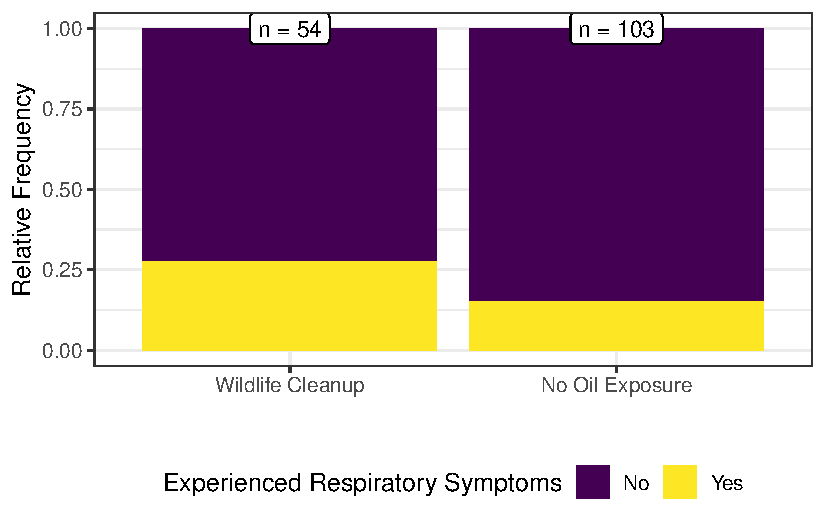
\includegraphics[width=0.8\textwidth,height=\textheight]{./images/fig-recaplanguage-deepwater-plot-1.pdf}

}

\caption{\label{fig-recaplanguage-deepwater-plot}The risk of developing
adverse respiratory symptoms for volunteers assigned to clean wildlife
is higher than that for those volunteers assigned to tasks which do not
have direct exposure to oil.}

\end{figure}%

As seen in Figure~\ref{fig-recaplanguage-deepwater-plot}, the rate of
adverse respiratory symptoms was larger in the group of volunteers
assigned to wildlife cleanup. Specifically, the rate of respiratory
symptoms was 1.79 times higher in the volunteers assigned to clean
wildlife compared to those assigned to tasks with no direct oil
exposure.

Notice that we reported the relative risk comparing the two groups as it
is directly tied to how we specified the hypotheses above. That is, the
statistic we report is governed by the parameter of interest; we compute
a value in the sample to estimate the corresponding value in the
population.

\begin{quote}
Distribution of the Sample: graphics and numerical summaries
characterize this distribution, informing us about the underlying
population. This is possible as long as the sample is representative of
the population.
\end{quote}

\section{Quantifying the Variability in the Estimate (Fundamental Idea
IV)}\label{quantifying-the-variability-in-the-estimate-fundamental-idea-iv}

While we have an estimate for the increased risk of adverse respiratory
symptoms for those volunteers assigned to clean wildlife, the estimate
has not taken into account sampling variability. In order to quantify
this variability, we use a bootstrap procedure to model the sampling
distribution of the relative risk. Observe that we focus on the sampling
distribution of the statistic that estimates the parameter of interest.

Recall that bootstrapping mimics the process for generating a sampling
distribution. In this case, ``repeating the study'' involves collecting
data from not one, but two groups. So, we must resample both from the 54
volunteers who were assigned to clean wildlife and the 103 volunteers
assigned to tasks not involving direct oil exposure. Each time we
resample, we ensure that we select 54 volunteers who clean wildlife and
103 who do not (mimicking the original study). We need the process of
the original study to be maintained. Each time we resample from these
groups, we compute the relative risk and retain this value.
Figure~\ref{fig-recaplanguage-sampling-distribution} shows the model for
the sampling distribution for the relative risk comparing these two
groups. Again, it is important to note that we are not generating
\emph{new} data; we are \emph{resampling} (or \emph{reusing}) the
original sample.

\begin{figure}

\centering{

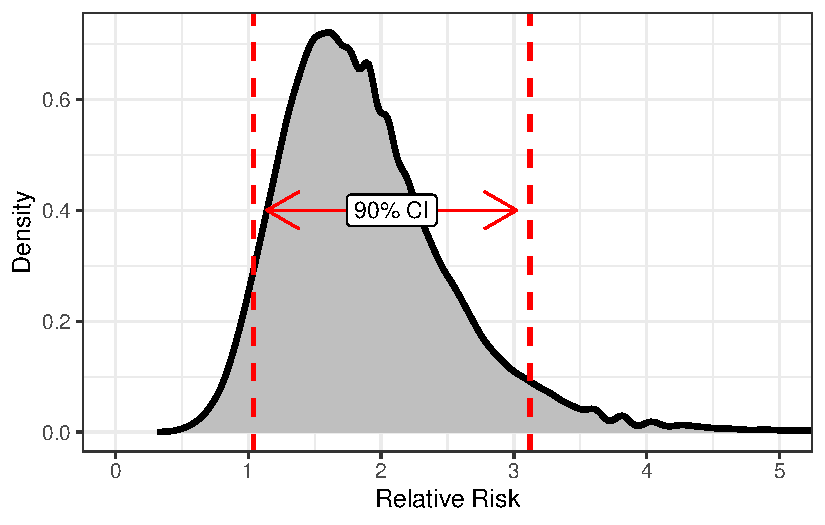
\includegraphics[width=0.8\textwidth,height=\textheight]{./images/fig-recaplanguage-sampling-distribution-1.pdf}

}

\caption{\label{fig-recaplanguage-sampling-distribution}Model of the
sampling distribution for the relative risk comparing volunteers
assigned to clean wildlife to volunteers assigned to tasks not involving
oil exposure. The model was developed via bootstrapping using 50000
replications.}

\end{figure}%

The study suggests that volunteers assigned to clean wildlife are 1.79
times (90\% CI = (1.04, 3.12)) more likely to experience adverse
respiratory symptoms compared to those volunteers assigned to tasks not
requiring direct exposure to oil. Our data is consistent with volunteers
assigned to clean wildlife being at increased risk compared to those who
do not have direct exposure to oil.

\begin{quote}
Sampling Distribution: allows us to quantify the variability in the
statistic and provide an interval estimate for the parameter which
incorporates this variability.
\end{quote}

\section{Quantifying the Evidence (Fundamental Idea
V)}\label{quantifying-the-evidence-fundamental-idea-v}

In order to quantify the departure of the data from our working
assumption that the risk is for those assigned to clean wildlife is no
more than that for those assigned to tasks without direct oil exposure,
we rely on a model for the null distribution and compute a p-value.

\begin{figure}

\centering{

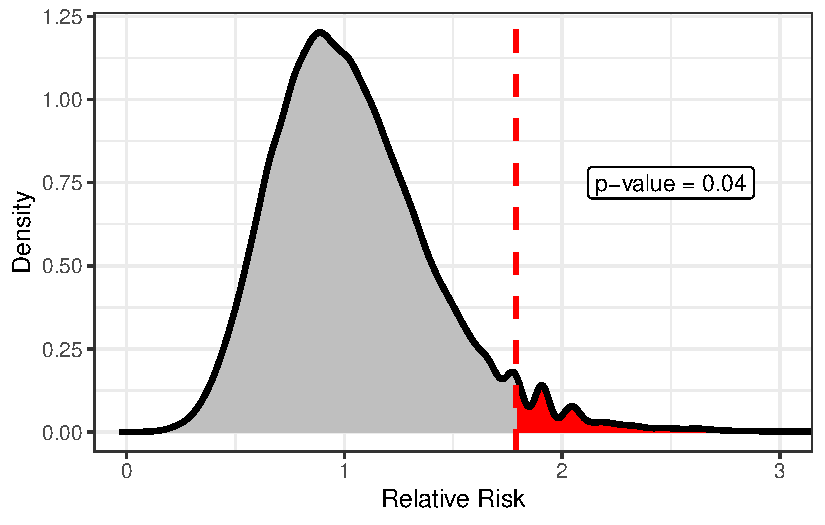
\includegraphics[width=0.8\textwidth,height=\textheight]{./images/fig-recaplanguage-null-distribution-1.pdf}

}

\caption{\label{fig-recaplanguage-null-distribution}Model of the null
distribution for the relative risk comparing volunteers assigned to
clean wildlife to volunteers assigned to tasks not involving oil
exposure. The null hypothesis assumed the two groups of volunteers had
the same risk. The null distribution was developed via bootstrapping
using 50000 replications.}

\end{figure}%

There is some (borderline weak) evidence (p = 0.04) to suggest that
volunteers exposed to oil have an increased risk of developing adverse
respiratory symptoms. Given the estimated level of this increased risk
(see the previous section for the confidence interval), we believe this
is something health officials should investigate further. It would be
worth investigating what aspects of the oil exposure may have led to the
increased risk to determine if it can be avoided in the future.

Note we are careful to not claim that the assignments have caused an
increase in the risk as this data is not from a controlled experiment.
This is one of the limitations of this analysis. However, if we are able
to assume the two groups are fairly similar with respect to other
attributes --- that is, there is no reason why people prone to
respiratory symptoms would be more likely to be assigned to wildlife
cleaning --- then we may have some reason to believe the results are
causal. We will wrestle more with these types of conclusions in future
units.

\begin{quote}
Null Distribution: allows us to quantify the level of evidence against a
particular claim or working hypothesis.
\end{quote}

\section{Summary}\label{summary}

Notice that our analysis moved through the \emph{Five Fundamental
Ideas}, and in doing so made use or referenced each of the four
components of the \emph{Distributional Quartet}. As we move through the
remainder of the text, we will explore how these frameworks are used in
various other analysis scenarios. As we do, we reveal additional
concepts involved in statistical modeling.

We admit that there are several other questions that may be raised by
the above analysis. This unit is meant to introduce the big concepts of
inference. We will concern ourselves more with the details as we
progress through the text.

\part{Unit II: Inference on the Overall Mean Response}

In Unit I, we developed the language and logic of statistical inference.
In this unit, we apply those concepts toward making statements about the
mean response of a variable. Throughout, we will take a modeling
perspective, using this specific context to develop key concepts around
statistical models. This will serve as a bridge between the big ideas in
Unit I and the more interesting models in the remainder of the text.

\chapter{Case Study: Birth Weights of Babies}\label{sec-casebabies}

The Centers for Disease Control and Prevention (CDC) --- using data
provided by the U.S. Department of Health and Human Services, National
Center for Health Statistics, the Division of Vital Statistics and the
CDC --- maintains a database on all babies born in a given
year\footnote{\url{http://wonder.cdc.gov/natality-current.html}}. This
database contains key metrics on each child born, including the weight
of the infant. Low birth weight can be indicative of poor health or
illness in children; and, high birth weight can be indicative of obesity
later in life. Researchers, therefore, use the database to examine links
between lifestyle choices of the parents (such as whether the mother
consumed alcohol during pregnancy) and birth weight of the infant.

Chihara and Hesterberg (2011) describe a random sample from this
database; specifically, the sample consists of 1009 babies born in North
Carolina during 2004. The babies each had a gestation period of at least
37 weeks (full term) and were single births (no twins, triplets, etc.).
For each birth in the sample, we have the following information:

\begin{itemize}
\tightlist
\item
  Age of the mother (in years).
\item
  Whether the mother is a current smoker.
\item
  Whether the mother used tobacco during the pregnancy.
\item
  Whether the mother used alcohol during the pregnancy.
\item
  Sex assigned to the child at birth (male or female).
\item
  Weight of the child at birth (grams).
\item
  Length of gestation (length of pregnancy, weeks).
\end{itemize}

A subset of the collected data is shown in
Table~\ref{tbl-casebabies-table}.

\begin{table}

\caption{\label{tbl-casebabies-table}Subset of a sample of 1009 babies
born in North Carolina during 2004.}

\centering{

\centering\centering
\resizebox{\ifdim\width>\linewidth\linewidth\else\width\fi}{!}{
\begin{tabular}[t]{rllrr}
\toprule
Subject ID & Age Range (years) & Assigned Sex of Baby & Weight of Baby (g) & Gestation (weeks)\\
\midrule
\cellcolor{gray!10}{\cellcolor{gray!10}{1}} & \cellcolor{gray!10}{\cellcolor{gray!10}{30-34}} & \cellcolor{gray!10}{\cellcolor{gray!10}{Male}} & \cellcolor{gray!10}{\cellcolor{gray!10}{3827}} & \cellcolor{gray!10}{\cellcolor{gray!10}{40}}\\
2 & 30-34 & Male & 3629 & 38\\
\cellcolor{gray!10}{\cellcolor{gray!10}{3}} & \cellcolor{gray!10}{\cellcolor{gray!10}{35-39}} & \cellcolor{gray!10}{\cellcolor{gray!10}{Female}} & \cellcolor{gray!10}{\cellcolor{gray!10}{3062}} & \cellcolor{gray!10}{\cellcolor{gray!10}{37}}\\
4 & 20-24 & Female & 3430 & 39\\
\cellcolor{gray!10}{\cellcolor{gray!10}{5}} & \cellcolor{gray!10}{\cellcolor{gray!10}{25-29}} & \cellcolor{gray!10}{\cellcolor{gray!10}{Male}} & \cellcolor{gray!10}{\cellcolor{gray!10}{3827}} & \cellcolor{gray!10}{\cellcolor{gray!10}{38}}\\
\addlinespace
6 & 35-39 & Female & 3119 & 39\\
\cellcolor{gray!10}{\cellcolor{gray!10}{7}} & \cellcolor{gray!10}{\cellcolor{gray!10}{20-24}} & \cellcolor{gray!10}{\cellcolor{gray!10}{Female}} & \cellcolor{gray!10}{\cellcolor{gray!10}{3260}} & \cellcolor{gray!10}{\cellcolor{gray!10}{40}}\\
8 & 20-24 & Male & 3969 & 40\\
\cellcolor{gray!10}{\cellcolor{gray!10}{9}} & \cellcolor{gray!10}{\cellcolor{gray!10}{20-24}} & \cellcolor{gray!10}{\cellcolor{gray!10}{Male}} & \cellcolor{gray!10}{\cellcolor{gray!10}{3175}} & \cellcolor{gray!10}{\cellcolor{gray!10}{39}}\\
10 & 25-29 & Female & 3005 & 39\\
\bottomrule
\end{tabular}}

}

\end{table}%

We might be interested in using this data to estimate the average birth
weight of an infant (carried to full term) born in North Carolina.

\chapter{Model for the Data Generating Process}\label{sec-meanmodels}

The numerical summaries of any study are subject to sampling
variability. That is, if we were to repeat the study with new subjects,
the statistics we compute would almost certainly change to some degree.
The key to feeling confident in our results is to quantify the
variability in our estimates; this was the rationale for developing a
model of the sampling distribution of a statistic
(Chapter~\ref{sec-samplingdistns}) and a model for the null distribution
of a statistic under a specified hypothesis
(Chapter~\ref{sec-nulldistns}). Often times, constructing such models
requires modeling the data-generating process as a precursor. As in any
other discipline, statistical models simplify the actual process being
modeled by making certain assumptions. In this chapter, we develop a
model for the data generating process that will help us make inference
about the mean of a single population. This will also serve as the
foundation for how we approach problems in other contexts moving forward
in the text.

\begin{tcolorbox}[enhanced jigsaw, breakable, titlerule=0mm, colframe=quarto-callout-note-color-frame, bottomtitle=1mm, opacityback=0, rightrule=.15mm, toptitle=1mm, arc=.35mm, bottomrule=.15mm, left=2mm, title=\textcolor{quarto-callout-note-color}{\faInfo}\hspace{0.5em}{Note}, leftrule=.75mm, coltitle=black, toprule=.15mm, colbacktitle=quarto-callout-note-color!10!white, colback=white, opacitybacktitle=0.6]

The word ``model'' is generic, and it applies to any representation of a
complex process. We will either explicitly describe the model we are
discussing (e.g., the model for the sampling distribution of a
statistic), or it should be clear from context. Regardless, it is
important to know which model is being referenced.

\end{tcolorbox}

\section{General Formulation}\label{general-formulation}

Consider dropping a tennis ball from the top of a 50-meter building and
recording the time required before the ball hits the ground. Applying
the principles learned in a first course in physics, we would be able to
compute the time precisely using the formula

\[\text{time} = \sqrt{\frac{2(\text{distance})}{9.8}}\]

where \(9.8 m/s^2\) is the acceleration due to gravity; further, this
formula works regardless of the mass of the object. Plugging 50 meters
into the equation yields a time of 10.2 seconds. If we were to drop a
second tennis ball from the same building, the formula tells us that it
will also take 10.2 seconds to hit the ground below. This is known as a
\textbf{deterministic} system since entering the same input results in
the same output each time.

\begin{definition}[Deterministic
Process]\protect\hypertarget{def-deterministic-process}{}\label{def-deterministic-process}

A process for which the output is completely determined by the input(s).
That is, the output can be determined with certainty.

\end{definition}

While we often think of the above formula as a ``law,'' we should
recognize that it is just a model. It simplifies extremely complex
processes involving the gravitational pull between objects; it makes
simplifying assumptions, such as the gravitational pull of your hand
when you release the ball is negligible compared to the gravitational
pull of the earth. More, the model works really well. Despite how well
it works, it does not always match reality. If we were to repeatedly
drop tennis balls from the same 50-meter building and record the time
before hitting the ground, we might find that the time differs slightly
from one ball to the next (it is true that these differences may be
negligible, but they would exist nonetheless).

There are several reasons why our observed responses do not line up
directly with those predicted by the above equation; for example, our
device for measuring time may be subject to some measurement error, a
strong gust of wind could alter the results (while the above equation
assumes no air resistance), or the person dropping the ball may have
inadvertently increased the initial velocity of the ball. These reasons,
and others, contribute to the observations not lining up exactly with
the model. That is, there is associated noise in the resulting
measurements. A model which incorporates this noise might be written as

\[\text{time} = \sqrt{\frac{2(\text{distance})}{9.8}} + \text{noise}\]

where the noise is not a known quantity. In fact, the noise is not a
constant as it varies from one observation to the next! As a result, the
output of the model (time) is no longer fully determined by the input
(distance); the output also depends on a random component, meaning the
same input could result in different outputs. This is known as a
\textbf{stochastic} model.

\begin{definition}[Stochastic
Process]\protect\hypertarget{def-stochastic-process}{}\label{def-stochastic-process}

A process for which the output cannot be predicted with certainty.

\end{definition}

In the above example, the deterministic model was extended to include a
stochastic component. This extension leads to our general formulation
for a statistical model used in this text:

\begin{equation}\phantomsection\label{eq-general-model}{
\text{Response} = \text{function}(\text{predictor variables, parameters}) + \text{noise}.
}\end{equation}

The response we observe is the result of two components:

\begin{itemize}
\tightlist
\item
  A deterministic component that is a function of predictor variables
  and unknown parameters. It is often this component on which we would
  like to make inference.
\item
  A stochastic component that captures the unexplained variability in
  the data generating process.
\end{itemize}

Since the noise is a random element which varies from one observation to
another, it has a distribution. We often place conditions on the
structure of this distribution to enable inference on the deterministic
component of the model. We discuss this later in the chapter.

This general model introduces what we will see as a theme in statistical
modeling --- partitioning the variability in the response. The model
says that part of the reason the response differs across units (or
subjects) is because those units have different values of the predictor,
and part of the reason the response differs across units is unexplained
random noise. Notice that the response is also governed by the value of
the parameters; however, as discussed in Chapter~\ref{sec-questions},
parameters are numeric constants, so do they not vary from one unit to
another. The above model just makes explicit how the parameters
characterize the population --- through the model for the data
generating process. As before, while the parameters are constants, they
are unknown. Our goal is to use data to make inference on the parameters
and therefore make inference on how the data is generated.

The overall goal of a statistical model is to give an explanation for
why the value of the response is what it is. How did it come to be? What
process generated the values we have observed? Our statistical model
says that these values have some deterministic component plus some
additional random noise we cannot explain.

We now simplify this general formulation for the specific case of making
inference on the population mean.

\begin{tcolorbox}[enhanced jigsaw, breakable, titlerule=0mm, colframe=quarto-callout-note-color-frame, bottomtitle=1mm, opacityback=0, rightrule=.15mm, toptitle=1mm, arc=.35mm, bottomrule=.15mm, left=2mm, title=\textcolor{quarto-callout-note-color}{\faInfo}\hspace{0.5em}{Note}, leftrule=.75mm, coltitle=black, toprule=.15mm, colbacktitle=quarto-callout-note-color!10!white, colback=white, opacitybacktitle=0.6]

We note that the above formulation assumes a quantitative response
variable, which is the focus of this text. If your response is
categorical, you can think of the response as simply the output of a
lottery where the number of outcomes and the likelihood of each outcome
is determined by a function of the predictor variables and parameters.

That is, the process is still stochastic, but the predictor variables
and parameters impact the likelihood of a particular value being
observed:

\[\text{Probability}(\text{Response is } y) = \text{function}(\text{predictor variables, parameters, } y)\]

\end{tcolorbox}

\section{Statistical Model for a Quantitative Response with No
Predictors}\label{statistical-model-for-a-quantitative-response-with-no-predictors}

Consider the Birth Weights Case Study described in
Chapter~\ref{sec-casebabies}.. Suppose we are interested in estimating
the average birth weight of infants (carried to full term) born in North
Carolina, the population from which our sample was taken. Our response
variable is the birth weight of the infant. Our question of interest is
not about the relationship of the birth weight to any other variable;
that is, there are no predictor variables being considered. But, that
does not mean the deterministic portion of our model is empty. We have a
parameter of interest: the average birth weight. This parameter lives in
the deterministic portion of the model. In particular, consider the
following model for the data generating process:

\[(\text{Birth Weight})_i = \mu + \varepsilon_i\]

where \(\mu\) represents the average birth weight of infants born in
North Carolina. In this model for the data generating process, the
function that represents deterministic component of
Equation~\ref{eq-general-model} takes the value \(\mu\), a constant. The
term \(\varepsilon_i\) is used to capture the random noise in the
\(i\)-th measurement; the subscript indexes the individual infants in
the sample, indicating that the noise in the birth weight for each
infant potentially differs. This \(\varepsilon_i\) captures the
difference between the birth weight for the \(i\)-th infant and the
overall mean birth weight of all infants. This model says that the birth
weight for the \(i\)-th infant is shifted (as a result of the noise
term) from the overall average birth weight \(\mu\). Notice that if
there were no noise in the system, the data generating process would say
that all infants have the same birth weight \(\mu\). However, due to
genetic variability, differences in the lifestyle of each mother, and
measurement error, \(\varepsilon_i\) is not a constant (noise does
exist), resulting in each subject having a different response.

Notice that the deterministic portion of the model describes the
\emph{mean response} through the parameter. This will be a running theme
in the models we consider in this text.

\begin{tcolorbox}[enhanced jigsaw, breakable, titlerule=0mm, colframe=quarto-callout-tip-color-frame, bottomtitle=1mm, opacityback=0, rightrule=.15mm, toptitle=1mm, arc=.35mm, bottomrule=.15mm, left=2mm, title=\textcolor{quarto-callout-tip-color}{\faLightbulb}\hspace{0.5em}{Big Idea}, leftrule=.75mm, coltitle=black, toprule=.15mm, colbacktitle=quarto-callout-tip-color!10!white, colback=white, opacitybacktitle=0.6]

The deterministic portion of the data generating process for
Equation~\ref{eq-general-model} describes the mean response; naturally,
it is often referred to as the mean response function. Note that the
mean response function is governed by parameters.

\end{tcolorbox}

Certainly, this model for the data generating process is a simplified
version of reality. Instead of capturing the impact of genetics or the
impacts of lifestyle choices made by the infant's mother on the infant's
birth weight, we simply allow those impacts to enter the random noise
component of the model. This does not make the model for the data
generating process incorrect; instead, it simply means our model will
not explain the variability in the response. In later chapters we will
begin to address this limitation. However, it is worth noting now that
all models for the data generating process are simplified versions of
reality, but that does not mean they are not helpful.

When the model for the data generating process does not contain a
predictor variable, we are saying that the only source of variability in
the response is random noise.

\begin{tcolorbox}[enhanced jigsaw, breakable, titlerule=0mm, colframe=quarto-callout-tip-color-frame, bottomtitle=1mm, opacityback=0, rightrule=.15mm, toptitle=1mm, arc=.35mm, bottomrule=.15mm, left=2mm, title=\textcolor{quarto-callout-tip-color}{\faLightbulb}\hspace{0.5em}{Big Idea}, leftrule=.75mm, coltitle=black, toprule=.15mm, colbacktitle=quarto-callout-tip-color!10!white, colback=white, opacitybacktitle=0.6]

The stochastic component of a statistical model captures the unexplained
variability due to natural variability in the population or measurement
error in the response.

\end{tcolorbox}

\begin{tcolorbox}[enhanced jigsaw, breakable, titlerule=0mm, colframe=quarto-callout-important-color-frame, bottomtitle=1mm, opacityback=0, rightrule=.15mm, toptitle=1mm, arc=.35mm, bottomrule=.15mm, left=2mm, title=\textcolor{quarto-callout-important-color}{\faExclamation}\hspace{0.5em}{Data Generating Process for Single Mean Response}, leftrule=.75mm, coltitle=black, toprule=.15mm, colbacktitle=quarto-callout-important-color!10!white, colback=white, opacitybacktitle=0.6]

In general, given a quantitative response variable and no predictors,
our model for the data generating process is

\begin{equation}\phantomsection\label{eq-single-mean}{(\text{Response})_i = \mu + \varepsilon_i}\end{equation}

where \(\mu\) represents the average response in the population, the
parameter of interest.

\end{tcolorbox}

It is worth pointing out that we have two ``models'' at this point: a
model for the data generating process and a model for the sampling
distribution of a statistic. The model for the data generating process
is used to develop a model for the sampling distribution (or null
distribution) of a statistic. It is the second model that is actually
necessary in order to conduct inference; the model for the data
generating process is simply a stepping stone to the model of interest.

\section{Conditions on the Error
Distribution}\label{conditions-on-the-error-distribution}

In our model for the data generating process we incorporated a component
\(\varepsilon\) to capture the noise observed in the response. Since the
error is a random variable (stochastic element), we know it has a
distribution. We typically impose a certain structure to this
distribution through the assumption of specific conditions. The more
conditions we impose, the easier it is to construct an analytical model
for the sampling distribution of the corresponding statistic. However,
the more conditions we impose, the less applicable our model is in a
general setting. More importantly for our discussion, the conditions we
impose dictate how we conduct inference (the computation of a confidence
interval or p-value).

\begin{tcolorbox}[enhanced jigsaw, breakable, titlerule=0mm, colframe=quarto-callout-note-color-frame, bottomtitle=1mm, opacityback=0, rightrule=.15mm, toptitle=1mm, arc=.35mm, bottomrule=.15mm, left=2mm, title=\textcolor{quarto-callout-note-color}{\faInfo}\hspace{0.5em}{Note}, leftrule=.75mm, coltitle=black, toprule=.15mm, colbacktitle=quarto-callout-note-color!10!white, colback=white, opacitybacktitle=0.6]

Why we need conditions on the stochastic portion of a model can be
confusing at first. Think of it this way: saying a term is ``random'' is
just too broad. It is like saying ``I am thinking of a number. What
number?'' There are too many choices to even have a hope of getting it
correct. We need structure (boundaries, conditions) on the problem.
Placing conditions on what we mean by ``random'' is like saying ``I am
thinking of a whole number between 1 and 10.'' Now, we have a problem we
can at least attack with some confidence.

\end{tcolorbox}

The first condition we consider is that the noise attributed to one
observed unit is \textbf{independent} of the noise attributed to any
other unit observed. That is, the amount of error \(\varepsilon\) in any
one response is unrelated to the error in any other response observed.
In context, the error in the birth weight of one infant is unrelated to
the error in the birth weight of any other infant. It is easiest to
understand this condition by examining a case when the condition would
not hold.

\begin{definition}[Independence]\protect\hypertarget{def-independence}{}\label{def-independence}

Two random variables are said to be independent when the likelihood that
one random variable takes on a particular value does not depend on the
value of the other random variable.

Similarly, two observations are said to be independent when the
likelihood that one observation takes on a particular value does not
depend on the value of the other observation.

\end{definition}

\begin{example}[Tire Rotation
Timing]\protect\hypertarget{exm-tire-rotation}{}\label{exm-tire-rotation}

Suppose we are conducting a study to estimate the amount of time, on
average, required for a novice technician to complete a tire rotation on
an automobile. We gather a sample of 25 novice technicians. We have the
first technician complete a tire rotation, allowing the other
technicians to watch, and record the time required to complete the task.
We then have the second technician complete a tire rotation, again
allowing the other technicians to watch, and record the time required to
complete the task. We continue in this way until we have recorded the
time required to complete a tire rotation for each of the 25
technicians.

We could model the data generating process for this as

\[(\text{Time})_i = \mu + \varepsilon_i\]

where \(\mu\) is the average time required to complete a tire rotation
for a novice technician. We might estimate the parameter \(\mu\) with
\(\frac{1}{25}\sum_{i=1}^{25} (\text{Time})_i\), the sample mean time
for the 25 observed technicians.

\end{example}

In Example~\ref{exm-tire-rotation}, it would \emph{not} be reasonable to
assume the errors are independent of one another. Since each technician
is able to observe the prior technicians, it is plausible that each
technician's performance is dependent on their observations (they are
learning tricks by watching others go before them). As a result, the
amount of noise in one technician's time is related to the amount of
noise in the next technician's time. Requiring independence among
observations prohibits these types of situations.

A second condition we consider is that the error for each subject is
\textbf{identically distributed}. This ensures that every student
essentially belongs to the same population.

\begin{definition}[Identically
Distributed]\protect\hypertarget{def-identically-distributed}{}\label{def-identically-distributed}

A set of random variables is said to be identically distributed if they
are from the same population.

Similarly, a set of observations is said to be identically distributed
if they share the same data generating process.

\end{definition}

Practically, this condition means that we do not have a systematic
component which is causing our population to be different from what we
expected. As an example, let's return to
Example~\ref{exm-tire-rotation}.

\begin{example}[Tire Rotation Timing,
Continued]\protect\hypertarget{exm-tire-rotation-alt}{}\label{exm-tire-rotation-alt}

Suppose we are conducting a study to estimate the amount of time, on
average, required for a novice technician to complete a tire rotation on
an automobile. We gather a sample of 25 novice technicians. All
technicians are permitted to begin training in the facility. During the
first week of training, we have the first technician complete a tire
rotation and record the time required to complete the task. During the
second week of training, we have the second technician complete a tire
rotation and record the time required to complete the task. We continue
in this way until we have recorded the time required to complete a tire
rotation for each of the 25 technicians.

Again, we might posit the same model for the data generating process as
in Example~\ref{exm-tire-rotation}, and we might estimate the average
time in the same way.

\end{example}

It would \emph{not} be reasonable to assume the errors across all
observations are from the same underlying population in
Example~\ref{exm-tire-rotation-alt}. As the technicians are continuing
their training over time, the group under study is changing over time. A
technician with 10 weeks of training should not be expected to perform
in the same way as a technician with 1 week of training. The
observations are being drawn from a population that is changing over
time. Therefore, we could not say that the underlying distribution is
identical for each observation.

While there are many other conditions we might consider imposing on the
data generating process, these two conditions (independence and
identically distributed) are sufficient for modeling the sampling
distribution of the sample mean (our statistic of interest here) using
the bootstrap process we described in Chapter~\ref{sec-samplingdistns}.
In future chapters, we will consider the impact of adding additional
conditions or relaxing these conditions.

\begin{tcolorbox}[enhanced jigsaw, breakable, titlerule=0mm, colframe=quarto-callout-note-color-frame, bottomtitle=1mm, opacityback=0, rightrule=.15mm, toptitle=1mm, arc=.35mm, bottomrule=.15mm, left=2mm, title=\textcolor{quarto-callout-note-color}{\faInfo}\hspace{0.5em}{Note}, leftrule=.75mm, coltitle=black, toprule=.15mm, colbacktitle=quarto-callout-note-color!10!white, colback=white, opacitybacktitle=0.6]

While not all authors make the distinction, we distinguish between a
``condition'' and an ``assumption.'' A \emph{condition} is a
mathematical requirement for justifying the statistical theory on which
we are relying. However, in practice, we are never able to guarantee a
condition is satisfied.

As a result, we will need to make certain \emph{assumptions} about the
data generating process. In future units, we will see how we determine
which assumptions are reasonable. At this point, we simply emphasize
that the assumptions we make govern the process by which we model the
sampling distribution.

\end{tcolorbox}

Throughout this section, we have been discussing the conditions placed
on distribution of the error term --- the stochastic portion of the
model. We emphasize that these conditions are placed on the
\emph{distribution}, not the values themselves. Further, notice that
Equation~\ref{eq-single-mean} states the response is formed by taking
the error and shifting it by the constant \(\mu\); as a result, the
distribution of the responses is simply a shifted version of the
distribution of the error terms. Figure~\ref{fig-meanmodels-shift}
illustrates this for a hypothetical population. Since the distribution
of the response is just a shifted version of the distribution on the
errors, any conditions placed on the distribution of the errors can be
translated to statements on the distribution of the response.

\begin{figure}

\centering{

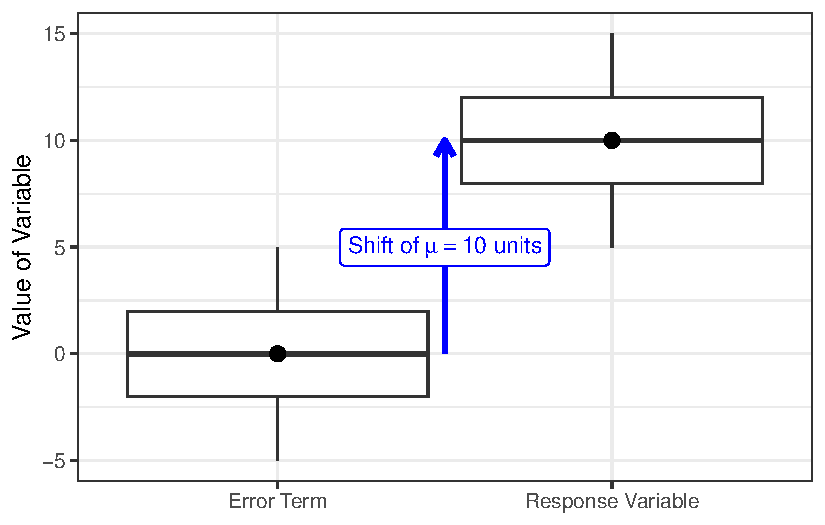
\includegraphics[width=0.8\textwidth,height=\textheight]{./images/fig-meanmodels-shift-1.pdf}

}

\caption{\label{fig-meanmodels-shift}Relationship between the
distribution of the response and the distribution of the error term in
the model for the data generating process involving a single mean
response.}

\end{figure}%

\begin{tcolorbox}[enhanced jigsaw, breakable, titlerule=0mm, colframe=quarto-callout-note-color-frame, bottomtitle=1mm, opacityback=0, rightrule=.15mm, toptitle=1mm, arc=.35mm, bottomrule=.15mm, left=2mm, title=\textcolor{quarto-callout-note-color}{\faInfo}\hspace{0.5em}{Note}, leftrule=.75mm, coltitle=black, toprule=.15mm, colbacktitle=quarto-callout-note-color!10!white, colback=white, opacitybacktitle=0.6]

For the model described in Equation~\ref{eq-single-mean}, stating

\begin{itemize}
\tightlist
\item
  the errors in the response for one observation is independent of the
  error in the response for all other observations, and
\item
  the errors in the response are identically distributed
\end{itemize}

is equivalent to stating

\begin{itemize}
\tightlist
\item
  the response for one observation is independent of the response for
  all other observations, and
\item
  the responses are identically distributed.
\end{itemize}

\end{tcolorbox}

Before leaving this chapter, it is worth noting that the introduction of
a model for the data generating process does not change any of the
fundamentals of inference we have previously discussed. This chapter
simply introduces a framework that allows us to unify all the methods we
discuss in this text.

\chapter{Estimating with Confidence a Single Mean}\label{sec-confint}

Consider the Birth Weight Case Study described in
Chapter~\ref{sec-casebabies}. In the previous chapter, we introduced the
following model for how birth weights for infants are generated:

\[(\text{Birth Weight})_i = \mu + \varepsilon_i\]

where \(\mu\) represents the average birth weight of infants born in
North Carolina. We also discussed imposing two conditions on the
distribution of the random error terms:

\begin{itemize}
\tightlist
\item
  The error in the birth weight for one infant is independent of the
  error in the birth weight for any other infant.\\
\item
  The errors in the birth weight for infants are identically
  distributed.
\end{itemize}

Within this model for the data generating process, \(\mu\) is an unknown
parameter of interest. Consider the following research goal associated
with this parameter:

\begin{quote}
On average, what is the birth weight of an infant born in North
Carolina?
\end{quote}

We can construct a point estimate of the parameter \(\mu\) with the
average birth weight of infants in our sample: 3448.26 g. The data is
graphically summarized in Figure~\ref{fig-confint-histogram}.

\begin{figure}

\centering{

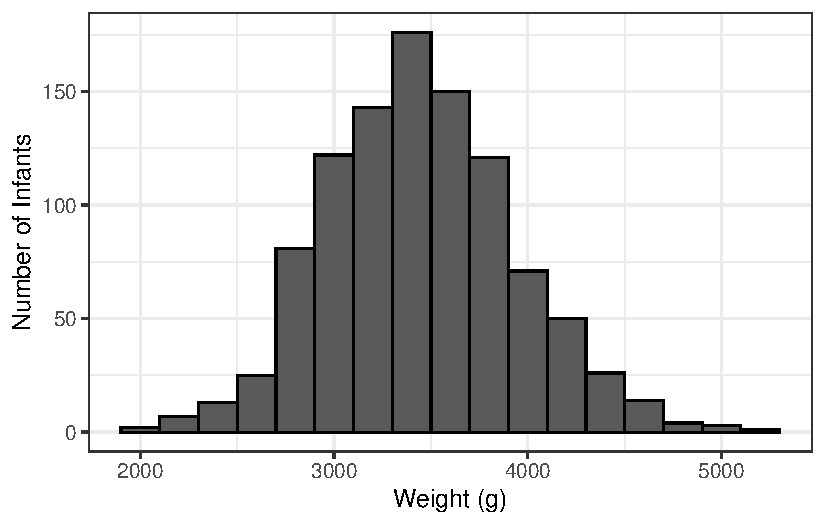
\includegraphics[width=0.8\textwidth,height=\textheight]{./images/fig-confint-histogram-1.pdf}

}

\caption{\label{fig-confint-histogram}Weight of a sample of full-term
infants born in North Carolina.}

\end{figure}%

In order to construct an estimate of \(\mu\) which incorporates the
variability in the sample mean, we must model the sampling distribution
of our estimate. The bootstrap procedure for this case would be

\begin{enumerate}
\def\labelenumi{\arabic{enumi}.}
\tightlist
\item
  Randomly sample, with replacement, 1009 records from the original
  sample.
\item
  For this bootstrap resample, compute the mean birth weight and retain
  this value.
\item
  Repeat steps 1 and 2 many (say 5000) times.
\end{enumerate}

This process is illustrated in Table~\ref{tbl-confint-bootstrap}. Each
row represents the birth weights for a single resample taken with
replacement from the original data. The final column is the computed
(and retained), sample mean from each resample (the bootstrap
statistic).

\begin{table}

\caption{\label{tbl-confint-bootstrap}Partial printout of first 10
bootstrap resamples and the resulting bootstrap statistic.}

\centering{

\centering
\begin{tabular}[t]{rrrlrrrr}
\toprule
Value 1 & Value 2 & Value 3 &         & Value 1007 & Value 1008 & Value 1009 & Boostrap Mean\\
\midrule
\cellcolor{gray!10}{3345} & \cellcolor{gray!10}{3572} & \cellcolor{gray!10}{3572} & \cellcolor{gray!10}{...} & \cellcolor{gray!10}{3827} & \cellcolor{gray!10}{3827} & \cellcolor{gray!10}{3119} & \cellcolor{gray!10}{3461.89}\\
3629 & 2892 & 3827 & ... & 4111 & 3374 & 2948 & 3476.69\\
\cellcolor{gray!10}{2495} & \cellcolor{gray!10}{3686} & \cellcolor{gray!10}{3827} & \cellcolor{gray!10}{...} & \cellcolor{gray!10}{3289} & \cellcolor{gray!10}{3544} & \cellcolor{gray!10}{3487} & \cellcolor{gray!10}{3428.90}\\
3856 & 3430 & 3771 & ... & 3487 & 3742 & 2665 & 3436.20\\
\cellcolor{gray!10}{3430} & \cellcolor{gray!10}{3119} & \cellcolor{gray!10}{4479} & \cellcolor{gray!10}{...} & \cellcolor{gray!10}{3686} & \cellcolor{gray!10}{3090} & \cellcolor{gray!10}{3005} & \cellcolor{gray!10}{3451.09}\\
\addlinespace
3289 & 3459 & 3827 & ... & 3600 & 3856 & 3260 & 3473.89\\
\cellcolor{gray!10}{2863} & \cellcolor{gray!10}{3345} & \cellcolor{gray!10}{3232} & \cellcolor{gray!10}{...} & \cellcolor{gray!10}{3345} & \cellcolor{gray!10}{3544} & \cellcolor{gray!10}{2948} & \cellcolor{gray!10}{3427.89}\\
3289 & 4026 & 3856 & ... & 4338 & 3771 & 3714 & 3435.78\\
\cellcolor{gray!10}{3175} & \cellcolor{gray!10}{3544} & \cellcolor{gray!10}{3771} & \cellcolor{gray!10}{...} & \cellcolor{gray!10}{3572} & \cellcolor{gray!10}{3515} & \cellcolor{gray!10}{3005} & \cellcolor{gray!10}{3419.37}\\
3260 & 3771 & 3742 & ... & 3572 & 4054 & 3033 & 3447.77\\
\bottomrule
\end{tabular}

}

\end{table}%

A plot of the resulting bootstrap sample means is shown in
Figure~\ref{fig-confint-samp-distn}. Notice that the x-axis is different
from that of Figure~\ref{fig-confint-histogram}. While a graphical
summary of the raw data is summarizing the weight of individual infants,
the model for the sampling distribution is summarizing the statistic we
compute in various resamples of the same size. In
Figure~\ref{fig-confint-samp-distn}, we are not keeping track of
individual infant weights but average weights for collections of 1009
infants.

\begin{figure}

\centering{

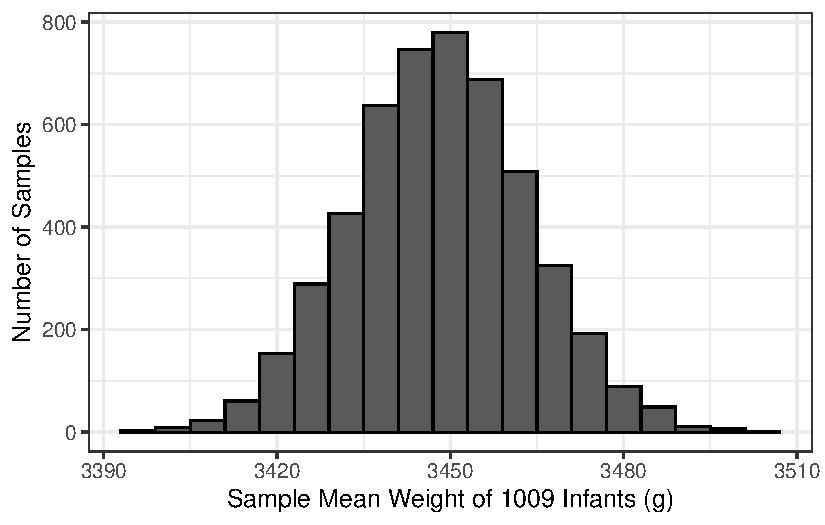
\includegraphics[width=0.8\textwidth,height=\textheight]{./images/fig-confint-samp-distn-1.pdf}

}

\caption{\label{fig-confint-samp-distn}Bootstrap model for the sampling
distribution of the average birth weight for a sample of 1009 infants
born in North Carolina.}

\end{figure}%

Using this model for the sampling distribution, we can then grab the
middle 95\% of values in order to construct a confidence interval for
the parameter of interest. This results in a 95\% confidence interval of
(3418.73, 3479). Based on this confidence interval, the data is
consistent with the birth weight of infants in North Carolina, on
average, being between 3418.73 and 3479; that is, these are the
reasonable values of the mean birth weight.

Notice that we are able to narrow down the reasonable values of the
parameter to a relatively small interval (a difference of about 60
grams). This is not because all babies in North Carolina have an
extremely similar birth weight. It is because we have a relatively large
sample, allowing us to have high confidence in our estimate of the
\emph{average} birth weight of an infant. The confidence interval does
not tell us where we expect an individual infant's birth weight to fall;
it only communicates what we are estimating the average birth weight of
all infants to be based on our observed sample.

Also, notice how much narrower the model for the sampling distribution
is compared to the distribution of the variable in the sample. Remember,
statistics have less variability than individual values. This also
illustrates why a confidence interval could never describe the fraction
of values in the population which fall within a certain range --- the
variability is not comparable because a sampling distribution has a
different x-axis than the distribution of the population or sample.

\chapter{Quantifying the Evidence for a Single Mean}\label{sec-teststat}

Consider the Birth Weight Case Study described in
Chapter~\ref{sec-casebabies}. In the previous chapter, we introduced
focused on estimating the mean response of a variable; in this chapter,
we consider testing a set of hypotheses involving the mean response.

In 2004, when the data for the Birth Weight Case Study was collected, an
infant was considered ``full term'' if it was born anytime between 37
and 42 weeks. However, in 2013 the American College of Obstetricians and
Gynecologists redefined ``full term''\footnote{\url{https://journals.lww.com/greenjournal/Fulltext/2013/11000/Committee_Opinion_No_579___Definition_of_Term.39.aspx}}
to mean an infant born anytime between 39 and 40 weeks. Consider the
following research question:

\begin{quote}
Does our study provide evidence that the average gestation time for
infants born in North Carolina exceeds 38 weeks (so that, on average,
babies are born full term by the new definition)?
\end{quote}

This question is captured by the following set of hypotheses:

\[H_0: \theta \leq 38 \qquad \text{vs.} \qquad H_1: \theta > 38\]

where \(\theta\) is the average gestation period (in weeks) of an infant
born in North Carolina. This parameter characterizes the following model
for the data generating process:

\[(\text{Gestation Period})_i = \theta + \varepsilon_i.\]

We will assume that the gestation period for one infant is independent
of the gestation period for any other infant and that this data is
representative of all infants born in North Carolina; this implies we
can assume the errors are independent and identically distributed.

We can estimate the parameter \(\theta\) with the average gestation
period for the babies in our sample: 39.11 weeks. We seek to quantify
the evidence against the null hypothesis summarized by this data.

In Chapter~\ref{sec-nulldistns}, we discussed the concept of the null
distribution of the statistic. Here, we are interested in modeling the
null distribution of the sample mean gestation for a sample of 1009
infants. Notice, just like when modeling the sampling distribution,
incorporating the sample size is an important aspect of our model.
Assuming the data is consistent with the above two conditions on the
distribution of the errors in the model for the data generating process,
we can construct a model of the null distribution using a bootstrap
procedure. Figure~\ref{fig-teststat-null-mean} illustrates this model
based on 5000 bootstrap replications.

\begin{figure}

\centering{

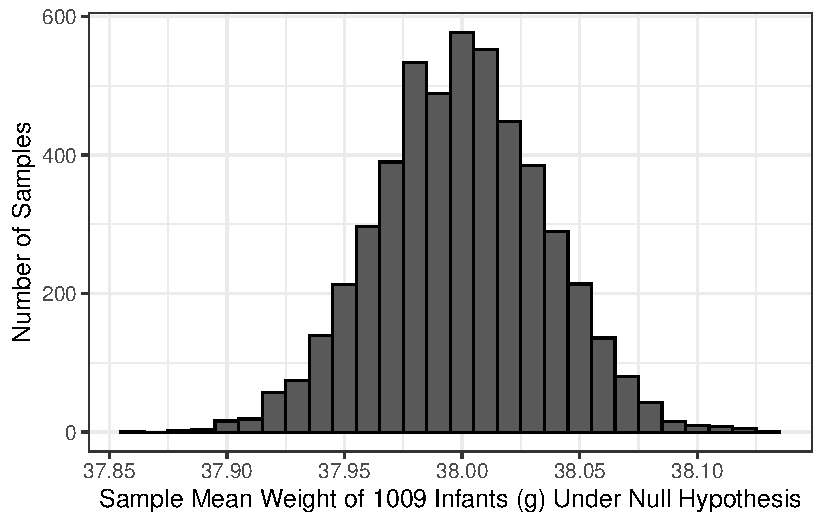
\includegraphics[width=0.8\textwidth,height=\textheight]{./images/fig-teststat-null-mean-1.pdf}

}

\caption{\label{fig-teststat-null-mean}Model of the null distribution of
the sample mean gestation period for a sample of 1009 infants. The model
is based on 5000 bootstrap replications under the null hypothesis that
the average gestation period is 38 weeks.}

\end{figure}%

Figure~\ref{fig-teststat-null-mean} was constructed using the following
procedure:

\begin{enumerate}
\def\labelenumi{\arabic{enumi}.}
\tightlist
\item
  Alter the sample to be representative of having come from a population
  in which the null hypothesis is true; in this case, the data was
  recentered to have a sample mean of 38.
\item
  Randomly sample, with replacement, 1009 records from the altered
  original sample.
\item
  For this bootstrap resample, compute the mean gestation period and
  retain this value.
\item
  Repeat steps 2 and 3 many (say 5000) times.
\end{enumerate}

The resulting simulated data is illustrated in
Table~\ref{tbl-teststat-bootstrap-mean}. Each row represents the
gestation periods for a single resample taken with replacement from the
altered original data. The final column is the computed (and retained),
sample mean from each resample. This is the bootstrap statistic
\emph{under the null hypothesis}.

\begin{longtable}[t]{rrrlrrrr}

\caption{\label{tbl-teststat-bootstrap-mean}Partial printout of first 10
bootstrap resamples under the null hypothesis and the resulting
bootstrap statistic.}

\tabularnewline

\toprule
Value 1 & Value 2 & Value 3 &  & Value 1007 & Value 1008 & Value 1009 & Boostrap Mean\\
\midrule
\cellcolor{gray!10}{36.88503} & \cellcolor{gray!10}{36.88503} & \cellcolor{gray!10}{39.88503} & \cellcolor{gray!10}{...} & \cellcolor{gray!10}{36.88503} & \cellcolor{gray!10}{36.88503} & \cellcolor{gray!10}{37.88503} & \cellcolor{gray!10}{37.96234}\\
36.88503 & 37.88503 & 37.88503 & ... & 39.88503 & 36.88503 & 35.88503 & 37.91278\\
\cellcolor{gray!10}{37.88503} & \cellcolor{gray!10}{37.88503} & \cellcolor{gray!10}{37.88503} & \cellcolor{gray!10}{...} & \cellcolor{gray!10}{38.88503} & \cellcolor{gray!10}{37.88503} & \cellcolor{gray!10}{39.88503} & \cellcolor{gray!10}{37.94747}\\
36.88503 & 37.88503 & 35.88503 & ... & 36.88503 & 38.88503 & 37.88503 & 38.02577\\
\cellcolor{gray!10}{36.88503} & \cellcolor{gray!10}{36.88503} & \cellcolor{gray!10}{37.88503} & \cellcolor{gray!10}{...} & \cellcolor{gray!10}{38.88503} & \cellcolor{gray!10}{37.88503} & \cellcolor{gray!10}{40.88503} & \cellcolor{gray!10}{38.00198}\\
\addlinespace
39.88503 & 38.88503 & 36.88503 & ... & 36.88503 & 37.88503 & 37.88503 & 38.03072\\
\cellcolor{gray!10}{38.88503} & \cellcolor{gray!10}{38.88503} & \cellcolor{gray!10}{36.88503} & \cellcolor{gray!10}{...} & \cellcolor{gray!10}{37.88503} & \cellcolor{gray!10}{36.88503} & \cellcolor{gray!10}{38.88503} & \cellcolor{gray!10}{38.06938}\\
36.88503 & 35.88503 & 39.88503 & ... & 36.88503 & 38.88503 & 37.88503 & 38.00396\\
\cellcolor{gray!10}{37.88503} & \cellcolor{gray!10}{36.88503} & \cellcolor{gray!10}{37.88503} & \cellcolor{gray!10}{...} & \cellcolor{gray!10}{37.88503} & \cellcolor{gray!10}{35.88503} & \cellcolor{gray!10}{35.88503} & \cellcolor{gray!10}{37.96234}\\
39.88503 & 37.88503 & 35.88503 & ... & 36.88503 & 35.88503 & 36.88503 & 37.99802\\
\bottomrule

\end{longtable}

Notice that the null distribution is centered on 38; this is not an
accident. Recall that sampling distributions are centered on the true
value of the parameter; since a null distribution is just the sampling
distribution of a statistic when the parameter is equal to the null
value (in this case 38), the null distribution should be centered on the
null value. That is, the null distribution is designed to be centered on
the null value in the hypotheses. In order to determine if our sample is
consistent with our expectations, we overlay our observed sample mean
(\(\widehat{\theta} = 39.11\)) on our model for the null distribution.
Since this value is in the far right tail of the null distribution (off
the edge of the graph in this case), our sample is \emph{inconsistent}
with the null distribution. This tells us that if the average gestation
period of an infant was only 38 weeks, we would not have expected to
observe a sample mean of \(\widehat{\theta} = 39.11\) or higher in a
sample of 1009 infants. Since our data is not consistent with our
expectations, our study provides evidence that the population from which
our sample was drawn has an average gestation period larger than 38
weeks.

\section{Standardized Statistics}\label{standardized-statistics}

In the above discussion, we compared the observed sample mean to our
distribution of expected sample means if the null hypothesis were true.
We were essentially comparing \(\widehat{\theta}\) to 38 while
accounting for the sampling variability of our estimate
\(\widehat{\theta}\), the sample mean. This is a completely valid
approach to inference. In this section, we consider an equivalent
(conceptually), though alternative, approach which will provide a more
general framework for inference.

At its heart, hypothesis testing is about comparing two models for the
data generating process. So far, we have stated one of those models:

\[\text{Model 1}: \quad (\text{Gestation Period})_i = \theta + \varepsilon_i.\]

This is the data generating process under the alternative hypothesis in
which no restrictions are placed on the value of \(\theta\). However,
\emph{if} the null hypothesis is true, then the model for the data
generating process simplifies to

\[\text{Model 0}: \quad (\text{Gestation Period})_i = 38 + \epsilon_i.\]

This may not seem like a simpler model, but it is because there are less
unknown parameters; specifically, Model 0 has no parameters. A null
hypothesis essentially places further restrictions on the data
generating process. A hypothesis test is then about comparing these two
models.

\begin{tcolorbox}[enhanced jigsaw, breakable, titlerule=0mm, colframe=quarto-callout-tip-color-frame, bottomtitle=1mm, opacityback=0, rightrule=.15mm, toptitle=1mm, arc=.35mm, bottomrule=.15mm, left=2mm, title=\textcolor{quarto-callout-tip-color}{\faLightbulb}\hspace{0.5em}{Big Idea}, leftrule=.75mm, coltitle=black, toprule=.15mm, colbacktitle=quarto-callout-tip-color!10!white, colback=white, opacitybacktitle=0.6]

Hypothesis testing is about comparing two potential models for the data
generating process. Specifically, we are asking whether a reduced model
is sufficient for explaining the data or if there is evidence a more
complex model is necessary.

\end{tcolorbox}

\begin{tcolorbox}[enhanced jigsaw, breakable, titlerule=0mm, colframe=quarto-callout-note-color-frame, bottomtitle=1mm, opacityback=0, rightrule=.15mm, toptitle=1mm, arc=.35mm, bottomrule=.15mm, left=2mm, title=\textcolor{quarto-callout-note-color}{\faInfo}\hspace{0.5em}{Note}, leftrule=.75mm, coltitle=black, toprule=.15mm, colbacktitle=quarto-callout-note-color!10!white, colback=white, opacitybacktitle=0.6]

You may be wondering why we chose the value 38 when writing Model 0
above. After all, the null hypothesis was \(H_0: \theta \leq 38\); so,
it is natural to wonder why we did not choose 37 or one of the other
infinite values below 38. In hypothesis testing, we choose to be as
conservative as possible. If we are to declare that the data is not
consistent with the null hypothesis, we want to be sure we are able to
say the data is not consistent with any part of the null hypothesis.

Recall that our observed statistic was \(\widehat{\theta} = 39.11\); so,
if we are able to state that we would not expect a sample mean gestation
period of 39.11 or larger if the mean gestation period in the population
is 38, then surely we are able to state that we would not expect a
sample mean gestation period of 39.11 or larger if the mean gestation
period in the population is 37. That is, if 39.11 is statistically
discernible from 38, surely it is statistically discernible from 37 (or
any other value less than 38).

That is, when setting up our model for the data generating process under
the null hypothesis --- when modeling the null distribution of our
statistic --- we choose the null value because it is the hardest to
establish evidence against in a one-sided hypothesis test. If we can
statistically discern our statistic differs from the null value, we can
statistically discern our statistic differs from any value specified in
the null hypothesis. That allows us to confidently provide evidence
against the entire null hypothesis.

\end{tcolorbox}

Essentially, the null hypothesis we have been considering
(\(H_0: \theta \leq 38\)) is stating that Model 0 is sufficient for
explaining the data observed. And, the alternative hypothesis
(\(H_1: \theta > 38\)) is stating that Model 0 is not sufficient, and a
more complex model (Model 1) is necessary for explaining the data
observed. This is why we refer to hypothesis testing as assessing model
consistency. We are determining if there is evidence that the data is
inconsistent with a proposed model for the data generating process.

Intuitively, the two proposed models would be equivalent (Model 0 would
be sufficient for explaining the data) if they both performed similarly
in predicting a response. Model 1 would be preferred (Model 0 would not
be sufficient for explaining the data) if it performs better in
predicting the response. While this idea is intuitive, the process for
comparing the models is not --- we can assess ``prediction'' by the
amount of variability in the data. If Model 0 captures a similar amount
of variability in the response as Model 1, then it is reasonable that
Model 0 is sufficient.

For Model 0, the amount of variability can be quantified by

\[SS_0 = \sum_{i=1}^{n} \left[(\text{Gestation Period})_i - 38\right]^2.\]

That is, we are computing the total amount (summation) that the observed
responses deviate (the squared difference) from the proposed mean of 38.
For Model 1, the amount of variability can be quantified by

\[SS_1 = \sum_{i=1}^{n} \left[(\text{Gestation Period})_i - \widehat{\theta}\right]^2\]

where \(\widehat{\theta} = 39.11\), the observed sample mean. Here, we
are computing the total amount (summation) that the observed responses
deviate (the squared difference) from the ``best'' estimate for the
unknown mean response. Since Model 1 does not place any constraints on
the value of the parameter, we use our estimate from the sample.

Notice that these sums of squared (SS) terms are similar to the
definition of sample variance discussed in Chapter~\ref{sec-summaries},
without the scaling factor. The rationale for using these to assess
predictive ability of the model will be further discussed in
Chapter~\ref{sec-regquality}. Here, we simply note that they are
measuring a distance the observed data is from a mean; the difference is
whether that mean is unrestricted (and therefore estimated from the
data, Model 1) or restricted under the null hypothesis (Model 0). If
\(SS_0\) and \(SS_1\) were similar, then it would suggest that
\(\widehat{\theta}\) is close to the null value of 38, and
\(\widehat{\theta}\) differs from the null value only due to sampling
variability, which would be in line with the null hypothesis. If, on the
other hand, \(SS_0\) and \(SS_1\) differ substantially from one another,
it suggests \(\widehat{\theta}\) differs from the null value more than
we would expect due to variability alone. That is, if \(SS_0\) and
\(SS_1\) differ substantially from one another, it suggests that our
data is not something we would expect to observe under the null
hypothesis. Therefore, the difference in these two sums of squares gives
us a measure of the signal in the data against the null hypothesis. The
larger this difference, the stronger the signal.

However, the same signal can be more difficult to detect (or discern) in
the presence of a lot of background noise. Think about having a radio on
in the background of a party, and suppose the radio is set to a specific
volume. If there are not many people talking at the party, it is easy to
hear the radio; the signal is strong relative to the background noise.
However, if there are a lot of people talking at the party, the radio is
difficult to hear \emph{even though its volume hasn't changed}; the
signal is weak \emph{relative} to the background noise. A signal is more
difficult to locate if the background noise is elevated. The same
principle holds in data analysis.

Consider Figure~\ref{fig-teststat-signal-to-noise}. Suppose we want to
use each of these datasets (both containing a sample of size \(n = 20\))
to test the hypotheses:

\[H_0: \mu = 0 \qquad \text{vs.} \qquad H_1: \mu \neq 0\]

where \(\mu\) is the population mean. Both datasets have \emph{exactly}
the same observed sample mean response (the black diamond in the
figure). Therefore, it can be shown that the difference between \(SS_0\)
and \(SS_1\) is exactly the same for both datasets. However, just
visually, it should be clear that Dataset A provides stronger evidence
against the null hypothesis than Dataset B; that is, Dataset A is more
inconsistent with a mean of 0. The difference is the variability --- the
background noise.

\begin{figure}

\centering{

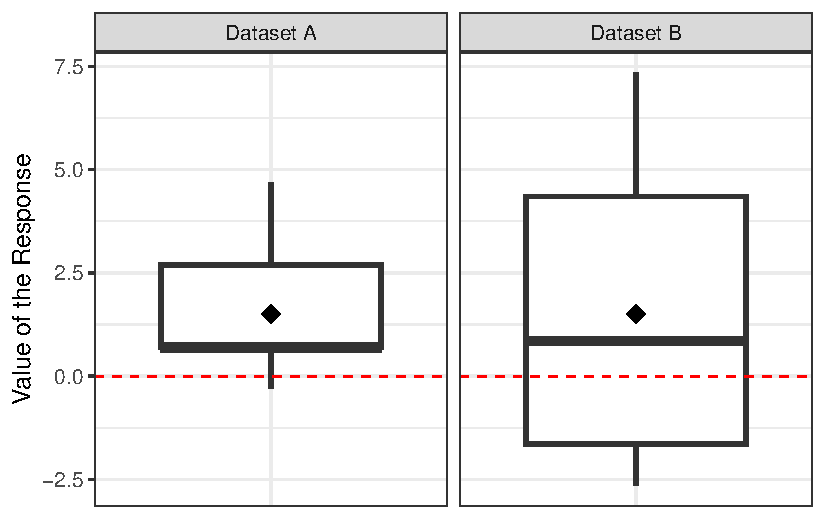
\includegraphics[width=0.8\textwidth,height=\textheight]{./images/fig-teststat-signal-to-noise-1.pdf}

}

\caption{\label{fig-teststat-signal-to-noise}Illustration of the need to
compare a signal to the noise in the data to assess its true strength.}

\end{figure}%

Therefore, when quantifying the strength of a signal in a statistical
analysis, it is common to measure the signal relative to the background
noise. Returning to our example for the Birth Weight Case Study, we have
that \(SS_0 - SS_1\) quantifies our signal. The noise is the variability
in the sample given by

\[s^2 = \frac{1}{n-1}\sum_{i=1}^{n} \left[(\text{Gestation Period})_i - \widehat{\theta}\right]^2,\]

the sample variance. We can examine our signal relative to the noise
using a signal-to-noise ratio,

\[T^* = \frac{SS_0 - SS_1}{s^2} = 963.2\]

for our example. Such signal to noise ratios are known as
\textbf{standardized statistics}.

\begin{definition}[Standardized (Test)
Statistic]\protect\hypertarget{def-standardized-test-statistic}{}\label{def-standardized-test-statistic}

Also, known as a test statistic, a standardized statistic is a ratio of
the signal in the sample to the noise in the sample. The larger the
standardized statistic, the stronger the evidence of a signal; said
another way, the larger the standardized statistic, the stronger the
evidence against the null hypothesis.

\end{definition}

\begin{tcolorbox}[enhanced jigsaw, breakable, titlerule=0mm, colframe=quarto-callout-note-color-frame, bottomtitle=1mm, opacityback=0, rightrule=.15mm, toptitle=1mm, arc=.35mm, bottomrule=.15mm, left=2mm, title=\textcolor{quarto-callout-note-color}{\faInfo}\hspace{0.5em}{Note}, leftrule=.75mm, coltitle=black, toprule=.15mm, colbacktitle=quarto-callout-note-color!10!white, colback=white, opacitybacktitle=0.6]

A standardized statistic is often referred to as a ``test statistic,''
or a ``standardized test statistic,'' because they are heavily used in
hypothesis testing.

\end{tcolorbox}

Of course, the natural question is ``when does a standardized statistic
become large enough?'' Just as we constructed the null distribution for
the observed sample mean in order to construct a distribution of our
expectations under the null hypothesis, we can construct a null
distribution of the standardized statistic to determine our expectations
of this ratio under the null hypothesis. Figure~\ref{fig-teststat-null}
provides a model for the null distribution of our standardized statistic
for the Birth Weight Case Study. This model for the null distribution is
constructed in the same way we constructed the model for the null
distribution of the sample mean except that instead of retaining the
sample mean from each resample, we compute and retain the standardized
statistic from each resample.

\begin{figure}

\centering{

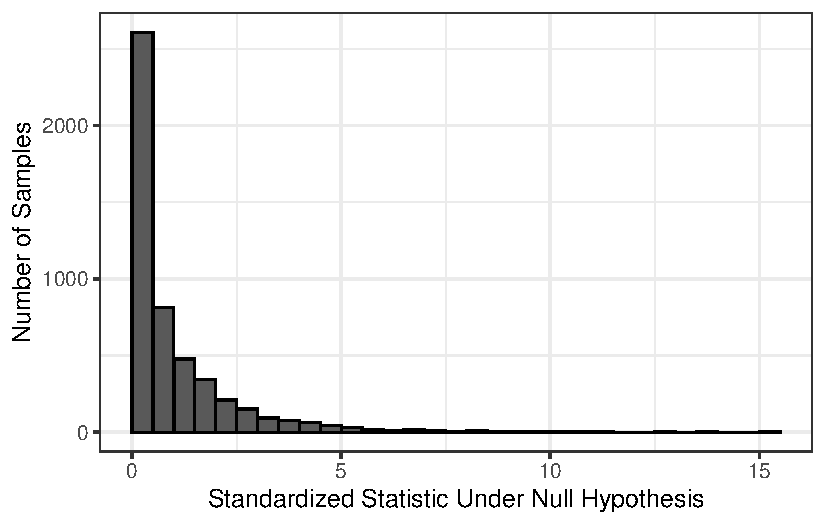
\includegraphics[width=0.8\textwidth,height=\textheight]{./images/fig-teststat-null-1.pdf}

}

\caption{\label{fig-teststat-null}Model of the null distribution of the
standardized statistic for a sample of 1009 infants. The model is based
on 5000 bootstrap replications under the null hypothesis that the
average gestation period is 38 weeks.}

\end{figure}%

Notice that using Figure~\ref{fig-teststat-null} we reach the same
conclusions as when we used Figure~\ref{fig-teststat-null-mean}. In
Figure~\ref{fig-teststat-null}, we see that our observed standardized
statistic of 963.2 is in the far right tail of the null distribution.
Therefore, our data is inconsistent with the null hypothesis. That is,
if the null hypothesis were true, it would be very unlikely to obtain a
sample which produced a standardized statistic this extreme or more so
due to sampling variability alone.

If our conclusions do not change, why the two different approaches? It
turns out there is some theory that says bootstrapping standardized
statistics tends to be a bit more stable computationally, and these
standardized statistics are a bit easier to model analytically using
probability theory (as we will later see). However, we introduce them
because it again provides a nice overarching framework that unifies
several of the approaches discussed in the text.

\begin{tcolorbox}[enhanced jigsaw, breakable, titlerule=0mm, colframe=quarto-callout-tip-color-frame, bottomtitle=1mm, opacityback=0, rightrule=.15mm, toptitle=1mm, arc=.35mm, bottomrule=.15mm, left=2mm, title=\textcolor{quarto-callout-tip-color}{\faLightbulb}\hspace{0.5em}{Big Idea}, leftrule=.75mm, coltitle=black, toprule=.15mm, colbacktitle=quarto-callout-tip-color!10!white, colback=white, opacitybacktitle=0.6]

Quantifying evidence to compare two models for the data generating
process can be done by comparing the signal in the data to the
background noise.

\end{tcolorbox}

Before moving on, we should note that there is not a unique standardized
statistic. Other standardized statistics are often reported; for
example, for hypothesis testing of a single mean response, the ratio

\[\frac{\sqrt{n}\left(\widehat{\theta} - \theta_0\right)}{s}\]

is often reported, where \(\theta_0\) is the value of the mean response
assumed under the null hypothesis.

It can be shown that many standardized statistics are related to one
another (for example, the one given here is the square root of the
standardized statistic reported previously). When the same conditions
are applied to the data generating process, various standardized
statistics yield the same conclusions. Again, we opt for the one
described earlier because it will provide continuity in the text.

\section{Computing the P-value}\label{computing-the-p-value}

Now that we have a model for the null distribution of the standardized
statistic, we can compute a p-value. The p-value is the probability of
observing a sample as or more extreme due only to sampling variability.
Our standardized statistic has the form

\[T^* = \frac{SS_0 - SS_1}{s^2}\]

If the sample were more extreme --- that is, if it produced a larger
signal --- then we would expect the difference between \(SS_0\) and
\(SS_1\) to be even larger. Therefore, larger values of the standardized
statistic present stronger evidence against the null hypothesis. When
looking at the null distribution of the standardized statistic,
computing the p-value corresponds to computing the area to the right of
the observed standardized statistic.

Looking back at Figure~\ref{fig-teststat-null}, our observed
standardized statistic is not even on the graphic, meaning the p-value
(the tail area) is essentially 0. The data therefore provides strong
evidence that the average gestation period of infants born in North
Carolina exceeds 38 weeks.

As stated in Chapter~\ref{sec-nulldistns}, we should never report a
p-value in isolation. We estimated the average gestation period of
infants born in North Carolina to be 39.11 weeks. Our p-value tells us
that we are able to statistically discern a difference between 39.11 and
the 38 weeks from the null hypothesis. This ability to statistically
discern this difference is in part due to the sample size of 1009
infants. To know whether this difference is meaningful, we would want to
discuss the results with an obstetrician. However, informally, the
increase of one week in the gestation period of an infant has a
significant impact on both the health of the infant and the life of the
mother (ask anyone who is 9 months pregnant!).

Finally, we take this opportunity to remind you that our conclusion is
only about the \emph{average} gestation period of infants. We make no
claim about how long any individual infant will be carried prior to
labor.

\part{Unit III: Modeling the Average Response as a Function of a
Continuous Predictor}

Unit I explored the language and logic of statistical inference, and
Unit II applied those concepts toward making inference on the mean
response of a single variable. Within this context, we developed the
idea of a statistical model for the data generating process, and
introduced the concept of a standardized statistic. We now refine these
ideas as we introduce the use of predictors in the data generating
process. Specifically, we model the average response as a linear
function of a single predictor.

\chapter{Case Study: Seismic Activity in Greece}\label{sec-casegreece}

At the intersection of the African plate, the Eurasia plate, and the
smaller Aegean plate, Greece is one of the most earthquake-prone regions
in the world. Between July 2016 and July 2017, Greece experienced 179
earthquakes; by contrast, the state of Texas experienced 28 over the
same span of time. In a region with such seismic activity, careful
consideration must be given to municipal construction. Understanding how
the motion experienced in a location is related to the soil properties
in the area or the magnitude and distance of an earthquake is important.

An article in the \emph{Journal of Earthquake Engineering} (Koutrakis et
al. 2002) examined seismic events in Greece occurring between 1978 and
1997. Of interest for construction is characterizing the ``strong ground
motion,'' when the earth shakes with enough force to cause damage to
infrastructure, with respect to the properties of a location. The study
recorded several measurements from 121 stations (representing 93
distinct seismic events)\footnote{The original article presented
  repeated measurements at each location. We present here only the first
  measurement from each location to simplify any analyses. Repeated
  measurements are discussed briefly later in the text; for a more
  thorough treatment of the subject, we recommend a course in Designed
  Experiments or Biostatistics. The dataset presented here corresponds
  to that presented in Navidi's ``Statistics for Engineers and
  Scientists'' (Chapter 8, Supplementary Exercise 22).}. The primary
variable of interest is the \emph{bracketed duration}, ``the time
interval {[}in seconds{]} between the first and last excursion of the
peak ground acceleration beyond a certain predefined level.'' For our
purposes, we only consider the data corresponding to a threshold of 2\%
of the acceleration due to gravity. A longer bracketed duration would
correspond to more time an area is exposed to violent shaking (and
therefore more time in which damage may occur). In addition to the
bracketed duration, the following measurements were available for each
observation:

\begin{itemize}
\tightlist
\item
  Moment Magnitude: a measure of the size of the earthquake; larger
  values indicate more severe earthquakes.
\item
  Epicentral Distance: distance (kilometers) from the epicenter of the
  earthquake to the location at which the measurement was taken.
\item
  Soil Condition: indicator of the type of soil present at the
  measurement site. Soil was categorized as one of three types -
  alluvium (soft, fine particles of clay, silt, sand, and gravel),
  intermediate soil conditions, or tertiary or older rock (those older
  than 2.58 million years).
\end{itemize}

The first 5 observations in the dataset are shown in
Table~\ref{tbl-casegreece-table}. In this unit, we are particularly
interested in characterizing the relationship between the bracketed
duration at a location and the magnitude of the corresponding
earthquake.

\begin{table}

\caption{\label{tbl-casegreece-table}Data for the first 5 observations
from a study characterizing seismic activity in Greece.}

\centering{

\centering
\begin{tabular}[t]{rrrl}
\toprule
Magnitude & Distance from Epicenter (km) & Bracketed Duration (s) & Soil Conditions\\
\midrule
\cellcolor{gray!10}{6.4} & \cellcolor{gray!10}{30} & \cellcolor{gray!10}{8.82} & \cellcolor{gray!10}{Soft}\\
5.3 & 6 & 4.31 & Intermediate\\
\cellcolor{gray!10}{5.6} & \cellcolor{gray!10}{15} & \cellcolor{gray!10}{5.74} & \cellcolor{gray!10}{Intermediate}\\
5.2 & 7 & 4.08 & Intermediate\\
\cellcolor{gray!10}{6.6} & \cellcolor{gray!10}{31} & \cellcolor{gray!10}{28.27} & \cellcolor{gray!10}{Soft}\\
\bottomrule
\end{tabular}

}

\end{table}%

\chapter{Myriad of Potential Questions}\label{sec-regquestions}

For the Seismic Activity Case Study, we are primarily interested in
characterizing the relationship between the bracketed duration at a
location and the magnitude of the corresponding earthquake. First, note
that this question is about the relationship between a quantitative
response (bracketed duration; see Definition~\ref{def-response}) and a
quantitative predictor (magnitude). Also note that the question is quite
broad. We might actually have one of the following more specific
questions in mind:

\begin{itemize}
\tightlist
\item
  In general, does the bracketed duration change as the magnitude
  changes?
\item
  If two earthquakes with different magnitudes occur in the same
  location, would we expect the same bracketed duration provided the
  locations have the same soil conditions?
\item
  Is the relationship between the bracketed duration and the magnitude
  different depending on the soil condition of where the measurement is
  taken?
\end{itemize}

These illustrate an array of potential questions we could address with
the data. Each represents a different emphasis that we might have in a
research question:

\begin{itemize}
\tightlist
\item
  Marginal Relationship: overall, do two variables tend to move together
  (are they correlated)?
\item
  Isolation of Effect: does a relationship exist after accounting for
  the effect of additional variables? Or, what is the effect ``above and
  beyond'' the effect of additional variables?
\item
  Interplay: how does the relationship between two variables change as a
  result of a third variable?
\end{itemize}

There is no right question to ask; each question examines a different
facet of the relationship between two quantitative variables. In this
unit, we will focus on questions of the first type. However, the
framework we introduce is broad enough to be extended to address each of
these types of questions. This may sound daunting, but keep in mind that
the fundamental ideas we discussed in Unit I and applied in Unit II will
continue to form the foundation of the analyses discussed in this unit;
namely,

\begin{itemize}
\tightlist
\item
  We are using a sample to say something about the underlying
  population.
\item
  In order to make inference, we will need a model for the sampling (or
  null) distribution of our statistic; as a stepping stone, we model the
  data generating process.
\item
  In order to form a standardized statistic of interest which measures
  the strength of the signal in the dataset, we think about variability.
\end{itemize}

The ideas remain the same; the context has changed.

There is one more thing we want to point out before moving on: any
relationships we observe are overall trends, not guaranteed to hold for
any single individual. Recall that in Unit II we emphasized that our
conclusions were about the mean response (the parameter of interest).
Specifically, even if we know the average response within the
population, due to variability, we do not expect every individual to
have that specific value for the response. This will continue in this
unit. If we observe, for example, that an increase in the magnitude is
associated with an increase in the bracketed duration, we are describing
an overall trend. It is highly likely there is some location for which
this trend does not hold, simply due to variability.

\chapter{Nature of Collecting Multivariable Data}\label{sec-regdata}

For the Seismic Activity Case Study, we are primarily interested in
characterizing the relationship between bracketed duration and the
magnitude of the earthquake. As we discussed in the previous chapter,
this general goal might be refined into one of many specific questions:

\begin{itemize}
\tightlist
\item
  In general, does the bracketed duration increase as the magnitude
  increases?
\item
  If two earthquakes with different magnitudes occur, would we expect
  the same bracketed duration provided the two locations of interest are
  the same distance from the epicenter?
\item
  Is the relationship between the bracketed distance and the magnitude
  different depending on the soil condition of where the measurement is
  taken?
\end{itemize}

Notice that these last two questions actually require knowledge of more
than just the bracketed duration and the magnitude of each seismic
event. In order to address the second question, we would also need the
distance from the center of the earthquake; in order to address the
third question, we also need the soil conditions of where the
measurement is taken. Often, research questions require knowledge of
more than just a single variable; such questions are
\textbf{multivariable}.

\begin{definition}[Multivariable]\protect\hypertarget{def-multivariable}{}\label{def-multivariable}

This term refers to questions of interest which involve more than a
single variable. Often, these questions involve many variables.
Multivariable models typically refer to a model with two or more
predictors.

\end{definition}

Consider going to the doctor because you are feeling ill.~The doctor
does not have you simply enter your most prominent symptom (fever, for
example) into a computer and then prescribe a medication based solely on
that single symptom. Instead, a good physician will review all symptoms
you are experiencing, as well as your medical history, other
medications, allergies, etc. The physician operates in a multivariable
world in which there are many contributing factors to a response.
Therefore, when you arrive for this hypothetical visit, they record
several variables that may be of interest.

Studies which collect several variables can be observational studies or
controlled experiments. If an observational study, we want to ensure the
sample of subjects is representative of the target population. Then, for
each individual, we simply record several variables. If a controlled
experiment, we randomly assign subjects to a particular ``treatment''
group; afterwards, we would measure the response in addition to other
variables. Notice that with the latter, subjects are randomly assigned
to only one of the variables; the remaining variables are simply
observed; while this could of course be extended, this is the most
common implementation.

\begin{tcolorbox}[enhanced jigsaw, breakable, titlerule=0mm, colframe=quarto-callout-note-color-frame, bottomtitle=1mm, opacityback=0, rightrule=.15mm, toptitle=1mm, arc=.35mm, bottomrule=.15mm, left=2mm, title=\textcolor{quarto-callout-note-color}{\faInfo}\hspace{0.5em}{Note}, leftrule=.75mm, coltitle=black, toprule=.15mm, colbacktitle=quarto-callout-note-color!10!white, colback=white, opacitybacktitle=0.6]

When a study is primarily interested in characterizing the relationship
between two or more quantitative variables, the data is typically from
an observational study.

\end{tcolorbox}

What we want to emphasize here is that how we collect the data has not
really changed from what we have discussed in previous units. The
primary difference is that we are very aware that we are collecting
several measurements on each subject. The critical element is that our
sample be representative of the target population if we want to apply
any findings to that population.

\chapter{Summarizing Multivariable Data}\label{sec-regsummaries}

For the Seismic Activity Case Study described in
Chapter~\ref{sec-casegreece}, we are primarily interested in
characterizing the relationship between the bracketed duration and the
magnitude of the corresponding earthquake. As we discussed in the
previous chapters, this broad question could be refined into a question
falling into one of three categories:

\begin{itemize}
\tightlist
\item
  Marginal Relationship: overall, does the bracketed duration and the
  magnitude of the corresponding earthquake tend to move together (are
  these two variables correlated)?
\item
  Isolation of Effect: is there an association between the bracketed
  duration and the magnitude of the corresponding earthquake after
  accounting for the impact of additional variables? That is, is there
  an association between the bracketed duration and the magnitude of the
  corresponding earthquake ``above and beyond'' the association with
  additional variables?
\item
  Interplay: how does the relationship between the bracketed duration
  and the magnitude of the corresponding earthquake depend on the type
  of soil?
\end{itemize}

As always, regardless of the question we ask, the key is developing
summaries which help to address that question.

\section{Characterizing the Marginal Relationship of Two Quantitative
Variables}\label{characterizing-the-marginal-relationship-of-two-quantitative-variables}

Suppose we are interested in the following question:

\begin{quote}
In general, does the bracketed duration tend to change as the magnitude
of the corresponding earthquake changes?
\end{quote}

This question is about the overall (marginal) relationship between these
two quantitative variables. Graphically, we can examine the relationship
between these two variables using a \emph{scatter plot}. The response is
placed on the y-axis and the predictor along the x-axis.
Figure~\ref{fig-regsummaries-magnitude} illustrates the relationship
between the bracketed duration at a location and the magnitude of the
corresponding earthquake.

\begin{figure}

\centering{

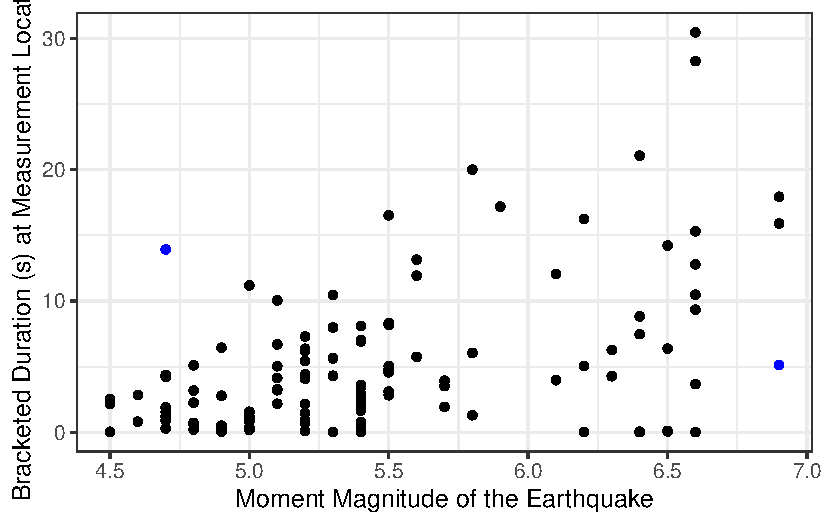
\includegraphics[width=0.8\textwidth,height=\textheight]{./images/fig-regsummaries-magnitude-1.pdf}

}

\caption{\label{fig-regsummaries-magnitude}Relationship between the
bracketed duration at a location in Greece and the magnitude of the
corresponding earthquake.}

\end{figure}%

Figure~\ref{fig-regsummaries-magnitude} highlights several facets of the
relationship. First, we note that as the magnitude of the event
increases, the bracketed duration also tends to increase. This is
intuitive --- as the size of the earthquake increases, the length of
time the ground shakes with extreme force increases. This is a
\emph{trend}; it is not a universal truth. For example, note the two
cases highlighted in blue; the observation with the larger magnitude has
a smaller bracketed duration, which is counter to the overall trend in
the graphic. The research objective was to characterize the overall
trend, not make global statements about all units in the population.
Figure~\ref{fig-regsummaries-magnitude} also reveals that as the
magnitude increases, the variability in the bracketed duration also
tends to increase. That is, for earthquakes of small magnitudes, it
seems fairly easy to anticipate the bracketed duration; however, the
bracketed duration is much more difficult to anticipate for larger
magnitudes.

A nice visual tool when exploring the relationship between two
quantitative variables is a \emph{smoothing spline}. The details of its
construction are beyond the scope of this text, but we can think of it
as representing where the average observed response is located for a
particular value of the predictor; when computing the average response,
information is borrowed form nearby points smoothing out the
relationship (hence the name). We do want to point out that this is an
exploratory device; we should be cautious about over-emphasizing
relationships we observe from the smoother.
Figure~\ref{fig-regsummaries-spline} illustrates a smoother relating the
length of the bracketed duration with the magnitude of the earthquake.
The addition of the spline confirms what we had previously stated about
the relationship appearing fairly linear (as the magnitude of the
earthquake increases so does the bracketed duration at a location). In
addition to the spline, there is a confidence band (generalization of a
confidence interval) around the line in order to convey the variability
in the estimated smoother.

\begin{figure}

\centering{

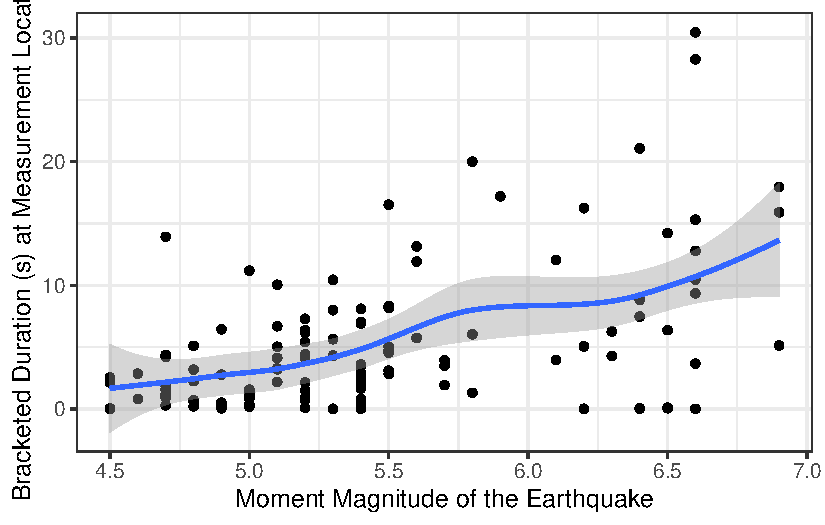
\includegraphics[width=0.8\textwidth,height=\textheight]{./images/fig-regsummaries-spline-1.pdf}

}

\caption{\label{fig-regsummaries-spline}Illustrating the use of a
smoothing spline to explore the relationship between the bracketed
duration and the magnitude of an earthquake for locations Greece.}

\end{figure}%

As we have seen, supplementing graphical summaries with numerical
summaries can help convey our message. As an example,
Figure~\ref{fig-regsummaries-spline} suggests there is a positive,
linear relationship between the bracketed duration and the magnitude of
the corresponding earthquake. But, can we quantify that relationship?
Consider Figure~\ref{fig-regsummaries-correlation}, which consists of
two hypothetical datasets. Both datasets illustrated exhibit a positive,
linear relationship between the response and predictor; however, that
relationship is much stronger (or more apparent) for Dataset A compared
to Dataset B. It would be nice to have a numeric summary which captured
this; such a metric is known as the \textbf{correlation coefficient}.

\begin{figure}

\centering{

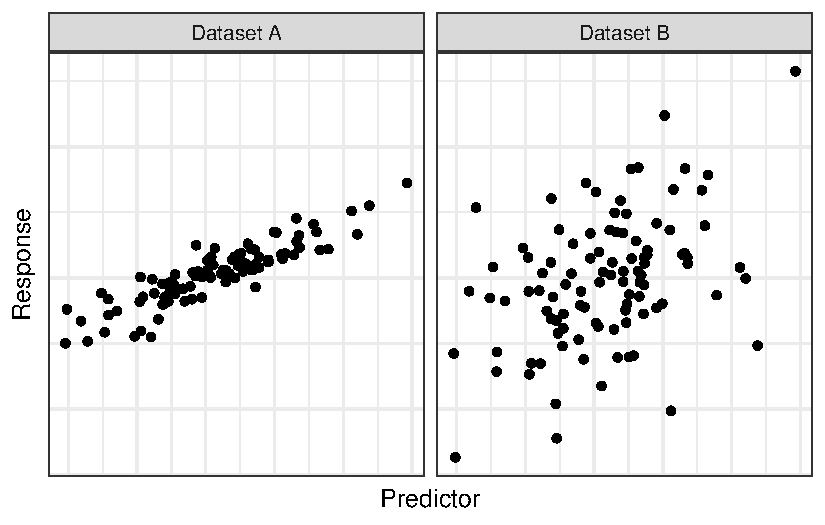
\includegraphics[width=0.8\textwidth,height=\textheight]{./images/fig-regsummaries-correlation-1.pdf}

}

\caption{\label{fig-regsummaries-correlation}The relationship between a
response and predictor for two hypothetical datasets; Dataset A exhibits
a stronger correlation between the response and predictor than Dataset
B.}

\end{figure}%

\begin{definition}[Correlation
Coefficient]\protect\hypertarget{def-correlation-coefficient}{}\label{def-correlation-coefficient}

A numerical measure of the \emph{strength} and \emph{direction} of the
\emph{linear} relationship between two quantitative variables.

The classical Pearson Correlation Coefficient \(r\) is given by the
following formula:

\[r = \frac{\sum_{i=1}^{n} \left(x_i - \bar{x}\right)\left(y_i - \bar{y}\right)}{\sqrt{\sum_{i=1}^n \left(x_i - \bar{x}\right)^2 \sum_{i=1}^n \left(y_i - \bar{y}\right)^2}}\]

where \(\bar{x}\) and \(\bar{y}\) represent the sample means of the
predictor and response, respectively.

\end{definition}

The correlation between the bracketed duration and the magnitude of an
earthquake in our sample is 0.497, indicating the two variables are
positively linearly related, though perhaps the relationship is not
strong.

\begin{tcolorbox}[enhanced jigsaw, breakable, titlerule=0mm, colframe=quarto-callout-note-color-frame, bottomtitle=1mm, opacityback=0, rightrule=.15mm, toptitle=1mm, arc=.35mm, bottomrule=.15mm, left=2mm, title=\textcolor{quarto-callout-note-color}{\faInfo}\hspace{0.5em}{Properties of the Correlation Coefficient}, leftrule=.75mm, coltitle=black, toprule=.15mm, colbacktitle=quarto-callout-note-color!10!white, colback=white, opacitybacktitle=0.6]

The Pearson Correlation Coefficient has the following key properties:

\begin{itemize}
\tightlist
\item
  It takes a value between -1 and 1.
\item
  Negative values mean that the variables tend to move in opposite
  directions.
\item
  Positive values mean that the variables tend to move in the same
  direction.
\item
  It is unitless and therefore unaffected by unit changes in the
  variables.
\end{itemize}

The biggest thing to remember is that a correlation coefficient measures
the strength of a \emph{linear} relationship. A correlation of 0 does
not mean that two variables are unrelated. It simply means they are not
linearly related.

\end{tcolorbox}

\section{Visualizing the Impact of a Third Variable on the Marginal
Relationship}\label{visualizing-the-impact-of-a-third-variable-on-the-marginal-relationship}

In the previous section, we stated that in our sample, the bracketed
duration tends to increase as the magnitude of the corresponding
earthquake increases. It is reasonable to ask the following question:

\begin{quote}
Is the relationship between the bracketed duration and the magnitude
different depending on the soil condition of where the measurement is
taken?
\end{quote}

That is, we want to determine the impact that a third variable (soil
condition) has on the relationship we have observed. While the bulk of
this unit will focus on inferential methods for the marginal
relationship, graphically assessing questions isolating a single
predictor or about the interplay of two predictors is fairly intuitive.
In order to add more depth to our graphical representations, we make use
of various features of the graphic --- the color, shape, and/or size of
the points used in plotting --- as well as facets (multiple graphics
each with a different subset of the data).
Figure~\ref{fig-regsummaries-color} uses color to distinguish between
the three possible types of soil conditions at each measurement
location. Notice the graphic allows us to both visualize the
relationship between the bracketed duration and the magnitude for each
soil condition but also facilitates our comparing these relationships
across soil conditions.

\begin{figure}

\centering{

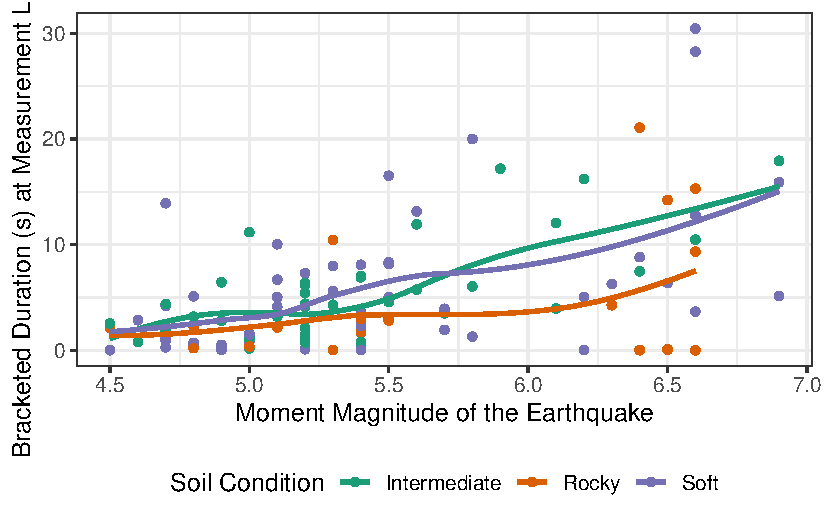
\includegraphics[width=0.8\textwidth,height=\textheight]{./images/fig-regsummaries-color-1.pdf}

}

\caption{\label{fig-regsummaries-color}Relationship of the bracketed
duration and the magnitude of the corresponding earthquake across across
various soil conditions.}

\end{figure}%

Figure~\ref{fig-regsummaries-color} illustrates that the relationship
between the bracketed duration at a location and the magnitude of the
corresponding earthquake is similar for both locations that have soft or
intermediate soil conditions. However, for locations with rocky
conditions, increases in the magnitude of the earthquake are associated
with less pronounced increases in the bracketed duration. This
potentially suggests that foundations on rocky soils are less subject to
the effects of large earthquakes, at least with respect to the amount of
time those areas are subject to extreme motion.

While our focus in this chapter has been on the scatter plot, our
emphasis remains the same as when we used simpler graphics in the first
unit --- summaries need to be constructed to address the question of
interest. And, regardless of the type of graphic, it communicates
information about how the distribution of the response.

\chapter{Bulding our Statistical Model}\label{sec-regmodel}

In Chapter~\ref{sec-meanmodels}, we introduced the statistical modeling
framework. In particular, our general model (see
Equation~\ref{eq-general-model}) for the data generating process was

\[\text{Response} = \text{function}(\text{predictor variables, parameters}) + \text{noise}.\]

Recall that this model has two components:

\begin{itemize}
\tightlist
\item
  A deterministic component which takes the form of a function of
  variables and unknown parameters. It is often this component on which
  we would like to make inference.
\item
  A stochastic component which captures the unexplained variability in
  the data generating process.
\end{itemize}

In the previous unit, we made use of this model, but we only scratched
the surface of its potential applications. In this unit, we explore some
of the capabilities of such a model. Specifically, we consider a model
for the data generating process such that the deterministic component is
a smooth function (specifically, a line) of potentially several
variables. In general, this model building process is known as
\textbf{regression}.

\begin{definition}[Regression]\protect\hypertarget{def-regression}{}\label{def-regression}

Used broadly, this refers to the process of fitting a statistical model
for the data generating process to observed data. More specifically, it
is a process of estimating the parameters in a data generating process
using observed data.

\end{definition}

\section{Statistical Model for A Quantitative Response and Quantitative
Predictor}\label{statistical-model-for-a-quantitative-response-and-quantitative-predictor}

Recall that in Chapter~\ref{sec-meanmodels}, we described a general
model for the data generating process of a quantitative response as a
function of a single parameter:

\[(\text{Response})_i = \mu + \varepsilon_i\]

where \(\mu\) represented the average response. We noted that this model
is fairly limited as it does not allow the response to depend on
additional information collected on each unit. In particular, we might
consider a model of the form

\begin{equation}\phantomsection\label{eq-regmodel-int-only}{(\text{Bracketed Duration})_i = \mu + \varepsilon_i}\end{equation}

for the data generating process of the bracketed duration. However, this
model does not allow the bracketed duration at a location to depend on
the magnitude of the corresponding earthquake. We would like to extend
it so that we can account for this additional information.

It is often easier to discuss modeling in the context of the graphics
used to visualize them. Consider the Seismic Activity Case Study
described in Chapter~\ref{sec-casegreece}. Let's begin with a broad
question:

\begin{quote}
In general, does the bracketed duration tend to change as the magnitude
of the corresponding earthquake changes?
\end{quote}

As we are interested in predicting the bracketed duration, we will treat
it as the response. In order to imagine what an appropriate model for
how the bracketed duration is generated as a function of the magnitude
of an earthquake, consider the graphical summary of how these variables
are related. As discussed in Chapter~\ref{sec-regsummaries}, we can use
a scatter plot to visualize the relationship between our response and
predictor. Figure~\ref{fig-regmodel-slr-plot} overlays a smoothing
spline (grey) on the observed data; however, it also includes a proposed
model (blue) for the data generating process for which the bracketed
duration is linearly related to the magnitude of the corresponding
earthquake.

\begin{figure}

\centering{

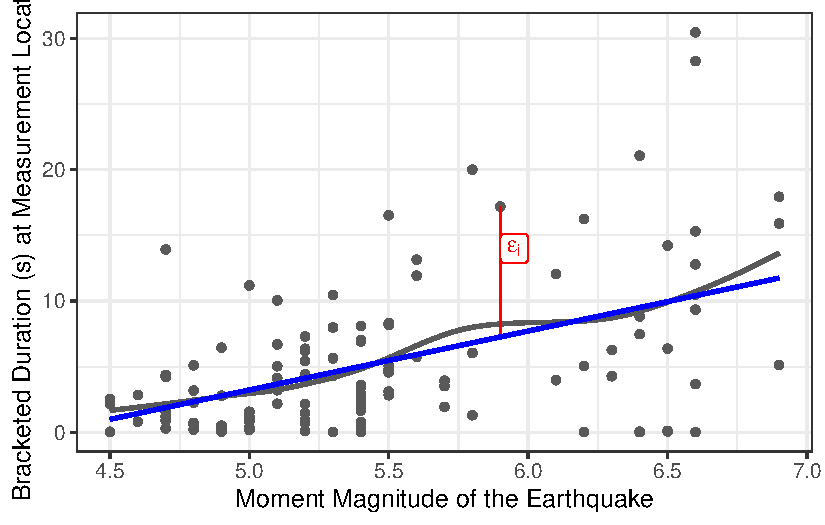
\includegraphics[width=0.8\textwidth,height=\textheight]{./images/fig-regmodel-slr-plot-1.pdf}

}

\caption{\label{fig-regmodel-slr-plot}Relationship between the bracketed
duration at locations across Greece and the magnitude of the
corresponding earthquake. A smoothing spline illustrates the overall
relationship, and a line overlayed represents a potential model for the
data generating process.}

\end{figure}%

Suppose we feel that this line is a good model for the data generating
process. Before proceeding, consider what this statement says. We are
not trying to say that the relationship explains every response we
observe. Instead, the relationship explains the underlying trend ---
what happens \emph{on average}. While not perfect, this linear
relationship at least appears plausible. Therefore, we replace \(\mu\)
in Equation~\ref{eq-regmodel-int-only} with the expression for a line;
this results in

\begin{equation}\phantomsection\label{eq-regmodel-slr}{(\text{Bracketed Duration})_i = \beta_0 + \beta_1 (\text{Magnitude})_i + \varepsilon_i}\end{equation}

where \(\beta_0\) represents the intercept of the line and \(\beta_1\)
the slope. Both the bracketed duration and the magnitude of the
corresponding earthquake are variables that are measures for each
observation. The terms \(\beta_0\) and \(\beta_1\) are unknown constants
(parameters) governing the model for the data generating process.

Observe that very few points in Figure~\ref{fig-regmodel-slr-plot}
actually fall on the proposed line in the graphic, which is to be
expected. This emphasizes the idea that the deterministic portion of the
model is not meant to fully capture a data generating process since
variability is inherent in any process. This is why statistical models
embed a deterministic component alongside a stochastic component --- to
capture the variability due to error or noise in the data generating
process.

The model suggests that the bracketed duration at a location is
primarily determined by the magnitude of the corresponding earthquake;
however, there is a component we cannot explain. That is, the model does
not explain why, for example, when an earthquake with a magnitude of 5.5
hits, all locations do not have the same bracketed duration. This noise
is picked up by the \(\varepsilon_i\) term in the model (as illustrated
for a single observation by the red line in
Figure~\ref{fig-regmodel-slr-plot}). The model is only capturing the
general trend. As in Chapter~\ref{sec-meanmodels}, we refine this model
for the data generating process further by placing additional conditions
on the random noise term in order to aid in conducting inference.

\begin{tcolorbox}[enhanced jigsaw, breakable, titlerule=0mm, colframe=quarto-callout-important-color-frame, bottomtitle=1mm, opacityback=0, rightrule=.15mm, toptitle=1mm, arc=.35mm, bottomrule=.15mm, left=2mm, title=\textcolor{quarto-callout-important-color}{\faExclamation}\hspace{0.5em}{Simple Linear Regression Model}, leftrule=.75mm, coltitle=black, toprule=.15mm, colbacktitle=quarto-callout-important-color!10!white, colback=white, opacitybacktitle=0.6]

For a quantitative response and a quantitative predictor, the general
form of the simple linear regression model is

\begin{equation}\phantomsection\label{eq-slr}{(\text{Response})_i = \beta_0 + \beta_1 (\text{Predictor})_i + \varepsilon_i}\end{equation}

where \(\beta_0\) and \(\beta_1\) are parameters governing the model for
the data generating process.

\end{tcolorbox}

\section{Estimating the Parameters}\label{estimating-the-parameters}

Recall the goal of statistics --- to use a sample to say something about
the underlying population. There is something intuitive about using the
sample mean as an estimate of the population mean; however, now we have
a model for the data generating process that has two parameters (the
intercept and the slope). We want a method that jointly estimates these
parameters.

Before discussing a specific estimation procedure, it is worth
emphasizing that our model for the data generating process has two
parameters. In equation Equation~\ref{eq-slr}, both \(\beta_0\) and
\(\beta_1\) are unknown constants governing the data generating process;
they are parameters. As discussed in Chapter~\ref{sec-questions},
parameters are \emph{unknown} values, and they will always be unknown.
We can use available data to \emph{estimate} these parameters (either
point estimates for interval estimates), and we can use available data
to determine if there is evidence the parameter falls outside of a
specific region (hypothesis testing), but we will \emph{never} be able
to definitely state the value of these parameters from a sample. As a
result, we do not ``compute'' the values of \(\beta_0\) and \(\beta_1\);
we can only estimate them. Indeed, nearly every scientist and engineer
is undoubtedly familiar with a line of ``best fit.'' We are emphasizing
here that any such line simply estimates the parameters in our model for
the data generating process.

We now turn to how such point estimates are constructed. Our model in
Equation~\ref{eq-slr} posits a linear deterministic portion for the data
generating process, and we want to use the data observed to estimate
what that relationship looks like. That is, we want to draw a line
through the points that gives the ``best fit.''
Figure~\ref{fig-regmodel-least-squares} illustrates this for a
hypothetical dataset; it compares two \emph{estimated relationships}.
Again, these are just estimates; neither represents the actual line from
which the data was generated. Examining the two estimated models,
something inside us knows that the blue line is preferred to the orange
line. The orange line does not seem to represent the pattern in the data
because it strays from the cloud of observed points. Intuitively, a
model that adequately describes the relationship between the two
variables should go through the observed points. Trying to formalize
this, we are saying we want a line that is somehow simultaneously as
close to all the data as possible.

\begin{figure}

\centering{

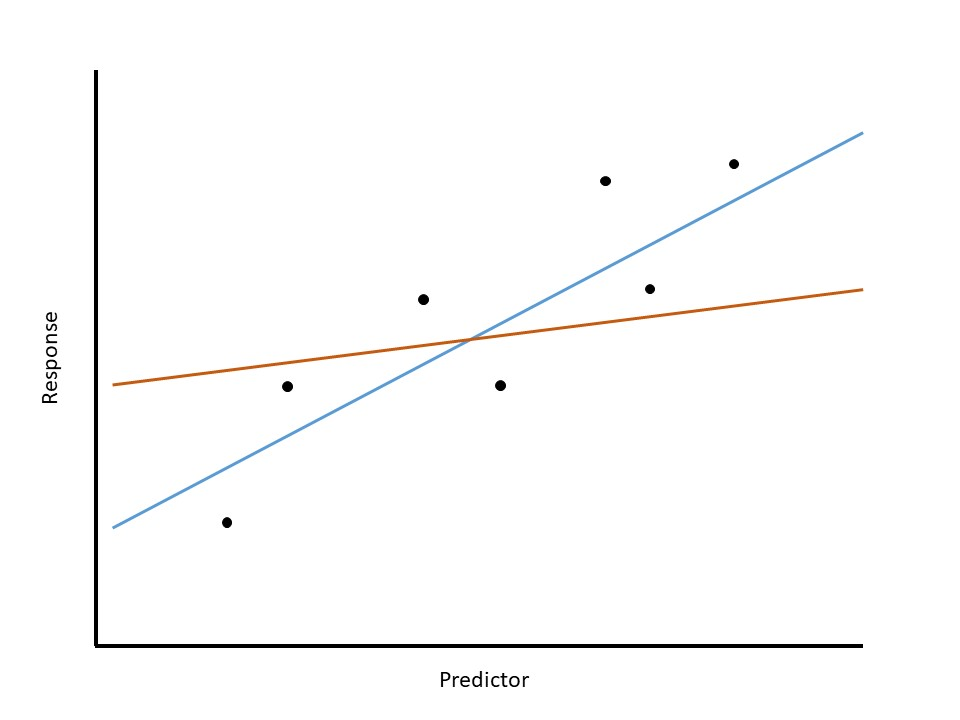
\includegraphics[width=0.8\textwidth,height=\textheight]{./images/RegModel-LeastSquares.jpg}

}

\caption{\label{fig-regmodel-least-squares}Illustration of two competing
estimates of a line which runs through the data.}

\end{figure}%

The most widely used method for accomplishing this goal, for estimating
the parameters in Equation~\ref{eq-slr}, is known as ``the method of
least squares.'' For this reason, the resulting parameter estimates are
often referred to as \textbf{least squares estimates}. This method
essentially chooses estimates for the parameters that minimize the
amount of error within the dataset.

\begin{definition}[Least Squares
Estimates]\protect\hypertarget{def-least-squares-estimates}{}\label{def-least-squares-estimates}

Often called the ``best fit line,'' these are the estimates of the
parameters in a regression model chosen to minimize the sum of squared
errors. Formally, for Equation~\ref{eq-slr}, they are the values of
\(\beta_0\) and \(\beta_1\) which minimize the quantity

\[\sum_{i=1}^n \left[(\text{Response})_i - \beta_0 - \beta_1(\text{Predictor})_{i}\right]^2.\]

The resulting estimates are often denoted by \(\widehat{\beta}_0\) and
\(\widehat{\beta}_1\).

\end{definition}

For those familiar with calculus, we can imagine finding the values of
the parameters which minimize the above quantity by taking partial
derivatives, setting those partial derivatives equal to 0, and solving
the resulting system of equations. In practice, the estimation is
carried out numerically using statistical software.

Estimation is often associated with statistics. However, the least
squares estimates are actually the result of a mathematical minimization
process. In order to make inference on the parameters, we need to
quantify the variability in those estimates --- that is the heart of a
statistical analysis. That is, the statistical aspect is moving into one
of the components of the \emph{Distributional Quartet}. In order to
construct a model for the sampling distribution of these statistics, we
place additional conditions on the stochastic portion of the model for
the data generating process. That is the focus of the next chapter.

\chapter{Conditions on the Error Term of a Regression
Model}\label{sec-regconditions}

In the previous chapter we developed a general model for the data
generating process of a quantitative response as a linear function of a
quantitative predictor:

\[(\text{Response})_i = \beta_0 + \beta_1 (\text{Predictor})_{i} + \varepsilon_i.\]

We also discussed a common method for estimating the parameters of this
model from a sample --- the method of least squares. However, if we are
to construct a model for the sampling distribution of these estimates we
must add some structure to the stochastic component \(\varepsilon\) in
the model. In this chapter, we focus on the most common conditions we
might impose and how those conditions impact the model for the sampling
and null distributions (and therefore the computation of a confidence
interval or p-value).

\section{Correctly Specified Model}\label{correctly-specified-model}

The first condition we consider is the most important. It states that
for every value of the predictor, the average error is 0.

\begin{tcolorbox}[enhanced jigsaw, breakable, titlerule=0mm, colframe=quarto-callout-note-color-frame, bottomtitle=1mm, opacityback=0, rightrule=.15mm, toptitle=1mm, arc=.35mm, bottomrule=.15mm, left=2mm, title=\textcolor{quarto-callout-note-color}{\faInfo}\hspace{0.5em}{Mean-0 Condition}, leftrule=.75mm, coltitle=black, toprule=.15mm, colbacktitle=quarto-callout-note-color!10!white, colback=white, opacitybacktitle=0.6]

The ``mean-0 condition'' states that for every value of the predictor,
the average error is 0.

\end{tcolorbox}

In practice, this condition implies that the deterministic portion of
the model for the data generating process that we have posited is
accurate; that is, it implies the \emph{form} of the model is
appropriate. For Equation~\ref{eq-slr}, this condition states that the
response is linearly related to the predictor.

There is a subtlety to this condition; the phrase ``for every value of
the predictor'' is crucial. Without this phrase, the condition would
simply state that the model may overestimate for some values of the
predictor, but that is balanced out by underestimating for other values
of the predictor. That is, the model for the deterministic portion can
be wrong everywhere, but those ``wrongs'' cancel each other out
(consider the orange line again in
Figure~\ref{fig-regmodel-least-squares}). Instead, we want the
deterministic portion of the model to be correct everywhere, for all
values of the predictor (consider the blue line again in
Figure~\ref{fig-regmodel-least-squares}).

There are two reasons we say that this is the most important condition:

\begin{enumerate}
\def\labelenumi{\arabic{enumi}.}
\tightlist
\item
  If this condition is violated, it says your model for the data
  generating process is fundamentally incorrect in its form. Generally,
  this is the result of ignoring some curvature in the relationship
  between the response and predictor or some important additional
  feature. If the functional form of the model for the deterministic
  portion is incorrect, you have to begin your modeling process over
  again.
\item
  This condition allows us to interpret the parameters of the model.
\end{enumerate}

That is, instead of \(\beta_0\) and \(\beta_1\) representing solely the
intercept and slope, we can interpret these parameters in the context of
the research objective.

\subsection{Interpreting the
Parameters}\label{interpreting-the-parameters}

In Chapter~\ref{sec-meanmodels}, we posited a model of the form

\[(\text{Response})_i = \mu + \varepsilon_i\]

where we said that \(\mu\) represented the average response. When we
impose the mean-0 condition in Equation~\ref{eq-slr}, we are stating
that given a value of the predictor, the average response is given by

\[\beta_0 + \beta_1 (\text{Predictor}).\]

That is, instead of considering the overall average response, we are
acknowledging that the average response may depend on the value of the
predictor. The mean-0 condition essentially tells us that the
deterministic portion of the model for the data generating process
represents the \emph{average} response for a specified value of the
predictor.

\begin{tcolorbox}[enhanced jigsaw, breakable, titlerule=0mm, colframe=quarto-callout-tip-color-frame, bottomtitle=1mm, opacityback=0, rightrule=.15mm, toptitle=1mm, arc=.35mm, bottomrule=.15mm, left=2mm, title=\textcolor{quarto-callout-tip-color}{\faLightbulb}\hspace{0.5em}{Big Idea}, leftrule=.75mm, coltitle=black, toprule=.15mm, colbacktitle=quarto-callout-tip-color!10!white, colback=white, opacitybacktitle=0.6]

The deterministic portion of a simple linear regression model specifies
the \emph{average} value of the response given the value of the
predictor.

\end{tcolorbox}

As an example, consider our model for the Seismic Activity Case Study
developed in Chapter~\ref{sec-regmodel}, which considered the bracketed
duration at a location as a function of the magnitude of the earthquake:

\[(\text{Bracketed Duration})_i = \beta_0 + \beta_1(\text{Magnitude})_i + \varepsilon_i.\]

If we are willing to assume that for earthquakes of any magnitude, the
average error in the bracketed duration is 0 (the mean-0 condition),
then earthquakes with a 5.0 magnitude have an \emph{average} bracketed
duration of

\[\beta_0 + \beta_1(5).\]

Similarly, earthquakes with a 6.0 magnitude have an \emph{average}
bracketed duration of

\[\beta_0 + \beta_1(6).\]

As we have mentioned, the deterministic portion of the model does not
specify the exact response for any individual unit; the deterministic
portion specifies the trend. We are now able to say that the ``trend''
we are modeling is the average response. Further, we can estimate this
average response by plugging in the least squares estimates
\(\widehat{\beta}_0\) and \(\widehat{\beta}_1\). Specifically, using the
method of least squares, the line of best fit was estimated as

\[(\text{Bracketed Duration}) = -19.19 + 4.48 (\text{Magnitude})\]

Therefore, we estimate the average bracketed duration for locations with
5.0 magnitude earthquakes to be 3.22 seconds, and we estimate the
average bracketed duration for locations with 6.0 magnitude earthquakes
to be 7.71 seconds. While we do not expect every location which has a
5.0 magnitude earthquake to have a bracketed duration of 3.22 seconds,
we expect the bracketed duration to vary about this length of time. This
is huge; it says that when we use a regression model to predict a
response, we are actually predicting the \emph{average} response. And,
it provides a direct interpretation of the parameters themselves.

Let's begin with the intercept term, \(\beta_0\). Notice that in our
model above, if we try to predict the bracketed duration for a location
with an earthquake which has a magnitude of 0, then our model returns
\(\beta_0\). In fact, for any regression model, the intercept
\(\beta_0\) is the value of the deterministic portion of the model when
the predictor in the model is set to 0, and we know that deterministic
portion is the average response.

\begin{tcolorbox}[enhanced jigsaw, breakable, titlerule=0mm, colframe=quarto-callout-note-color-frame, bottomtitle=1mm, opacityback=0, rightrule=.15mm, toptitle=1mm, arc=.35mm, bottomrule=.15mm, left=2mm, title=\textcolor{quarto-callout-note-color}{\faInfo}\hspace{0.5em}{Interpretation of the Intercept}, leftrule=.75mm, coltitle=black, toprule=.15mm, colbacktitle=quarto-callout-note-color!10!white, colback=white, opacitybacktitle=0.6]

Consider a regression model of the form Equation~\ref{eq-slr}; if we
impose the mean-0 condition, the intercept \(\beta_0\) represents the
\emph{average} response when the predictor is equal to 0. Note that the
resulting estimate may not be feasible; indeed, considering a predictor
of 0 may not even make sense in every context (e.g., an earthquake with
a magnitude of 0 is not an earthquake).

\end{tcolorbox}

For our particular example, our intercept is estimated to be -19.19;
this estimates the average bracketed duration for an earthquake with a
magnitude of 0. An earthquake with no magnitude is not an earthquake at
all; and, if there is no earthquake, we would not expect the ground to
undergo any duration of extreme motion. Further, even if a magnitude of
0 made sense, a negative duration does not.

When predictions for a model do not make logical sense, it is often the
result of \textbf{extrapolation}. We do not have any data on the
bracketed duration for locations which experienced an earthquake with a
magnitude less than 4.5. Therefore, we are using a model to predict for
a region over which the model was not constructed to operate. This is a
lot like using a screw driver to hammer a nail --- we are using a tool
to accomplish a task for which it was not designed. We should therefore
not be surprised when the tool fails. The primary reason extrapolation
is dangerous is that without data in a particular region, we have
nothing supporting that the posited model for the data generating
process will continue to hold in that region. We have illustrated this
when discussing the intercept, but extrapolation can occur in any region
for which there is no data. For this reason, unless you have strong
scientific justification for why a model will hold over all values of
the predictor, extrapolation should be avoided.

\begin{definition}[Extrapolation]\protect\hypertarget{def-extrapolation}{}\label{def-extrapolation}

Using a model to predict outside of the region for which data is
available.

\end{definition}

With an interpretation of the intercept \(\beta_0\), we now turn our
attention to the slope \(\beta_1\). Notice that based on our estimates
above, the average bracketed duration is 4.48 seconds longer for those
locations which experience a 6.0 magnitude earthquake compared to those
which experience a 5.0 magnitude earthquake, and this difference is the
value of the estimated slope. This is not a coincidence; 4.48 seconds is
the change in the average bracketed duration that is associated with a
1-unit increase in the magnitude of an earthquake. The slope is
essentially comparing the average response for two values of the
predictor that differ by 1 unit.

\begin{tcolorbox}[enhanced jigsaw, breakable, titlerule=0mm, colframe=quarto-callout-note-color-frame, bottomtitle=1mm, opacityback=0, rightrule=.15mm, toptitle=1mm, arc=.35mm, bottomrule=.15mm, left=2mm, title=\textcolor{quarto-callout-note-color}{\faInfo}\hspace{0.5em}{Interpretation of the Slope}, leftrule=.75mm, coltitle=black, toprule=.15mm, colbacktitle=quarto-callout-note-color!10!white, colback=white, opacitybacktitle=0.6]

Consider a regression model of the form Equation~\ref{eq-slr}; if we
impose the mean-0 condition, the slope \(\beta_1\) represents the
\emph{average} change in the response associated with a 1 unit
\emph{increase} in the predictor.

\end{tcolorbox}

\subsection{Embedding our Question in a Statistical
Framework}\label{embedding-our-question-in-a-statistical-framework}

Our first fundamental idea centers on the idea that the majority of
research questions can be framed in terms of a parameter within the
population. This seemed somewhat intuitive when the parameter was simply
the mean response. With parameters which are the slope and intercept of
a line, this seems less clear. However, the mean-0 condition provides
interpretations of the parameters, and this in turn ensures that our
questions of interest can be framed in terms of those parameters.
Consider the following question:

\begin{quote}
On average, are changes in the magnitude of an earthquake associated
with changes in the bracketed duration observed?
\end{quote}

Let's consider how we might write this in terms of a null and
alternative hypotheses. The mean-0 condition states that our form for
the deterministic portion of the model is correct. That is, imposing the
mean-0 condition means we believe the following model for the data
generating process is accurate:

\[(\text{Bracketed Duration})_i = \beta_0 + \beta_1(\text{Magnitude})_i + \varepsilon_i\]

The research question suggests we are looking for a relationship (which
we have posited to be linear \emph{if} it exists). Since a relationship
between the bracketed duration, on average, and the magnitude is what we
are seeking evidence for, the presence of such a relationship should be
captured by the alternative hypothesis. In turn, the null hypothesis
would capture the idea that the average bracketed duration does not
depend on the magnitude. That is, under the null hypothesis, magnitude
should not be present in the model at all; that is, our model would
reduce to

\[(\text{Bracketed Duration})_i = \beta_0 + \varepsilon_i.\]

This reduced model suggests that the bracketed duration does not change
at all as the magnitude changes; instead, the average bracketed duration
remains \(\beta_0\) for all values of the magnitude. This is essentially
a flat line, which comes from a slope of 0. That is, if the null
hypothesis is true --- that changes in the magnitude are not associated
with any changes in the bracketed duration --- then, under our proposed
model for the data generating process (which we believe has the correct
\emph{form} since we have imposed the mean-0 condition), then
\(\beta_1 = 0\). Said another way, under the null hypothesis, our model
for the data generating process of the bracketed duration should not
depend on the magnitude of the earthquake.

Therefore, our null and alternative hypotheses for the above research
question can be written as

\begin{quote}
\(H_0: \beta_1 = 0\)\\
\(H_1: \beta_1 \neq 0\)
\end{quote}

where \(\beta_1\) is the parameter linearly relating the bracketed
duration to the magnitude --- it is the average change in the bracketed
duration associated with a 1 unit increase in the magnitude.

\begin{tcolorbox}[enhanced jigsaw, breakable, titlerule=0mm, colframe=quarto-callout-tip-color-frame, bottomtitle=1mm, opacityback=0, rightrule=.15mm, toptitle=1mm, arc=.35mm, bottomrule=.15mm, left=2mm, title=\textcolor{quarto-callout-tip-color}{\faLightbulb}\hspace{0.5em}{Big Idea}, leftrule=.75mm, coltitle=black, toprule=.15mm, colbacktitle=quarto-callout-tip-color!10!white, colback=white, opacitybacktitle=0.6]

Setting the slope parameter to 0 in Equation~\ref{eq-slr} is associated
with saying that the predictor is not associated with the average
response in a linear fashion --- that it does not belong in the model.

\end{tcolorbox}

The interpretation of our parameters allows us to see that our research
questions are characterizing the relationship between the response and
the predictor, \emph{on average}. As in the previous unit, our questions
are about the average response; instead of looking at the overall
average, however, we are allowing it to depend upon a predictor.

This first condition on the error term --- holding the average error to
be 0 for all values of the predictor --- gives our parameters meaning.

\section{Independent Errors}\label{independent-errors}

The second condition we consider is that the noise attributed to one
observed individual is independent of the noise attributed to any other
individual observed. That is, the amount of error in any one
individual's response is unrelated to the error in any other response
observed. This is the same condition we introduced in
Chapter~\ref{sec-meanmodels}.

\begin{tcolorbox}[enhanced jigsaw, breakable, titlerule=0mm, colframe=quarto-callout-note-color-frame, bottomtitle=1mm, opacityback=0, rightrule=.15mm, toptitle=1mm, arc=.35mm, bottomrule=.15mm, left=2mm, title=\textcolor{quarto-callout-note-color}{\faInfo}\hspace{0.5em}{Independence Condition}, leftrule=.75mm, coltitle=black, toprule=.15mm, colbacktitle=quarto-callout-note-color!10!white, colback=white, opacitybacktitle=0.6]

The independence condition states that the error in one observation is
independent (see Definition~\ref{def-independence}) of the error in all
other observations.

\end{tcolorbox}

With just these first two conditions (that the average error is 0 for
all values of the predictors and the errors are independent of one
another), we can use a bootstrap algorithm in order to model the
sampling distribution of the least squares estimates of our parameters
(see Appendix~\ref{sec-app-theory}). However, additional conditions are
often considered.

\section{Same Degree of Precision}\label{same-degree-of-precision}

The third condition that is typically placed on the distribution of the
errors is that the variability of the errors is the same for all values
of the predictor. Practically, if this condition does not hold, our
response will be more precise in one region than in another. The
technical term for this condition is \emph{homoskedasticity}.

\begin{tcolorbox}[enhanced jigsaw, breakable, titlerule=0mm, colframe=quarto-callout-note-color-frame, bottomtitle=1mm, opacityback=0, rightrule=.15mm, toptitle=1mm, arc=.35mm, bottomrule=.15mm, left=2mm, title=\textcolor{quarto-callout-note-color}{\faInfo}\hspace{0.5em}{Constant Variance}, leftrule=.75mm, coltitle=black, toprule=.15mm, colbacktitle=quarto-callout-note-color!10!white, colback=white, opacitybacktitle=0.6]

Also called homoskedasticity, the constant variance condition states
that the variability of the errors is the same for all values of the
predictor.

\end{tcolorbox}

With this additional condition imposed, we are able to modify our
bootstrap algorithm when constructing a model for the sampling
distribution of the least squares estimates.

\section{Specific form of the Error
Distribution}\label{specific-form-of-the-error-distribution}

Up to this point in the text, we have discussed bootstrapping as the
tool for modeling the sampling distribution (or null distribution) of a
statistic. Bootstrapping results in an empirical (data-driven) model for
the sampling distribution. And, empirical models for distributions can
be unstable in small sample sizes. That is, our model for the sampling
distribution may change quite substantially from one sample to another.
To be clear, our modeling strategy approach takes into account the
sample size and communicates this uncertainty in the form of wider
confidence intervals. Nevertheless, this instability should be kept in
mind. In such cases, alternative bootstrap algorithms should be
considered.

An alternative to building an empirical model is to construct an
analytical model. While the term ``analytical'' as an alternative to
empirical might suggest the model is not data-driven, this is a
misnomer. The model for the sampling distribution of a statistic is
still based on the observed sample; the term ``analytical'' really means
that we can bypass the resampling component of a bootstrap procedure. In
particular, the information gained from bootstrapping (the shape and
spread of the sampling distribution) is obtained from relying on
statistical theory. An analytical approach generally comes from imposing
a fourth condition (common in engineering and scientific disciplines) on
the distribution of the errors.

\subsection{Modeling the Population}\label{modeling-the-population}

Before we delve into more detail, let's set the stage for the bigger
story being told. Recall that our goal is to say something about the
population using a sample. We have developed a process to address this
goal:

\begin{enumerate}
\def\labelenumi{\arabic{enumi}.}
\tightlist
\item
  Frame our question through a parameter of interest.
\item
  Collect data that allows us to estimate the parameter using the
  analogous statistic within the sample.
\item
  Summarize the variability in the data graphically.
\item
  Quantify the variability in the statistic through modeling the
  sampling distribution (or null distribution, whichever is
  appropriate).
\item
  Using the model for the sampling distribution, determine the
  reasonable values of the parameter; or, using the model for the null
  distribution, quantify the evidence in the sample.
\end{enumerate}

This process is presented through our \emph{Five Fundamental Ideas of
Inference} and the \emph{Distributional Quartet}. The key step in this
process is quantifying the variability by modeling the \emph{sampling
distribution} (or \emph{null distribution}, whichever is appropriate for
our research goal). We have described the construction of these models
empirically, through repeating the study by appropriately resampling the
data available and performing the analysis on each resample.

Our goal is still to model the sampling distribution; that is the key
inferential step. Instead of building an empirical model, we can
construct an exact analytical model through an additional step: modeling
the population directly.

\begin{tcolorbox}[enhanced jigsaw, breakable, titlerule=0mm, colframe=quarto-callout-tip-color-frame, bottomtitle=1mm, opacityback=0, rightrule=.15mm, toptitle=1mm, arc=.35mm, bottomrule=.15mm, left=2mm, title=\textcolor{quarto-callout-tip-color}{\faLightbulb}\hspace{0.5em}{Big Idea}, leftrule=.75mm, coltitle=black, toprule=.15mm, colbacktitle=quarto-callout-tip-color!10!white, colback=white, opacitybacktitle=0.6]

A model for the sampling distribution of a statistic can often be
obtained by modeling the distribution of the population.

\end{tcolorbox}

Notice yet another usage of the word ``model.'' We have discussed models
for the data generating process, and we have discussed models for the
sampling (or null) distribution of a statistic. Now, we are discussing a
model for the distribution of the population. As we will see, a model
for the distribution of the population is closely linked to the model
for the data generating process; as such, the model for the distribution
of the population is simply a stepping stone to the model for the
sampling distribution --- the key inferential step. It is important to
separate these steps. We are not interested in directly modeling the
population; we do it in order to construct a model for the sampling
distribution.

Just as with other conditions we have discussed, specifying a particular
model for the distribution of the population can allow us to depend on
some statistical theory; however, in practice, we are \emph{assuming}
this model for the distribution of the population is appropriate.

\subsection{The Normal Distribution}\label{the-normal-distribution}

Probability, a sub-field of mathematics which is used heavily in
statistical theory, is the discipline of modeling randomness. In
statistical theory, we make use of probability to model a distribution.
In order to get a feel for probability models, consider the following
example.

\begin{example}[Iris
Characteristics]\protect\hypertarget{exm-iris}{}\label{exm-iris}

The discipline of statistics began in the early 1900's primarily within
the context of agricultural research. Edgar Anderson was a researcher
investigating the characteristics of the iris. He had collected
measurements on over one hundred iris flowers, including their petal
length and width and their sepal length and width. The sepal is the area
(typically green) beneath the petal of a flower. It offers protection
while the flower is budding and then support for the petals after the
flower blooms.

\end{example}

Figure~\ref{fig-regconditions-iris-histogram} is a histogram of the
sepal width for the iris plants observed by Edgar Anderson; overlayed is
the density plot for the same dataset, which we have described as a
smoothed histogram. Both the histogram and the density plot are
empirical models of the distribution of the sepal width.

\begin{figure}

\centering{

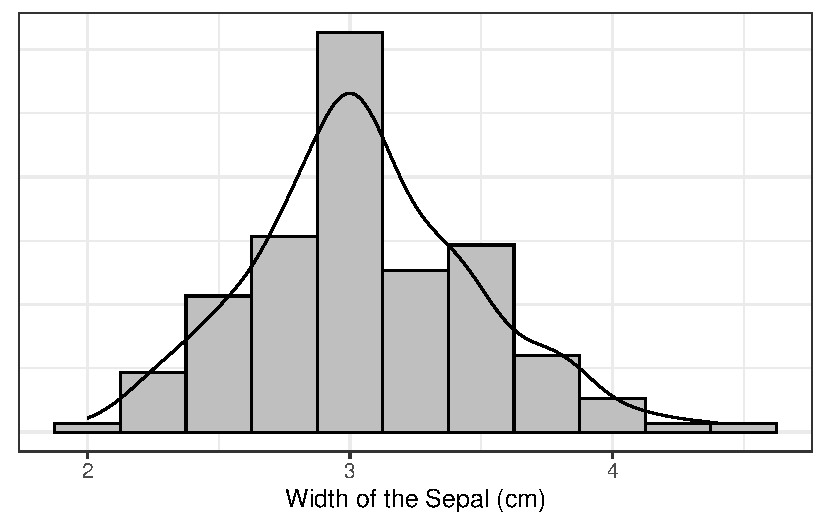
\includegraphics[width=0.8\textwidth,height=\textheight]{./images/fig-regconditions-iris-histogram-1.pdf}

}

\caption{\label{fig-regconditions-iris-histogram}Summary of the
distribution of sepal widths for a sample of irises.}

\end{figure}%

Probability models are analytical models for the distribution of a
variable. Instead of constructing a density using data alone, we posit a
functional form for the density. For example,
Figure~\ref{fig-regconditions-iris-normal} overlays the following
function on top of the the iris data:

\[f(x) = \frac{1}{\sqrt{0.380\pi}} e^{-\frac{1}{0.380}(x - 3.057)^2}.\]

\begin{figure}

\centering{

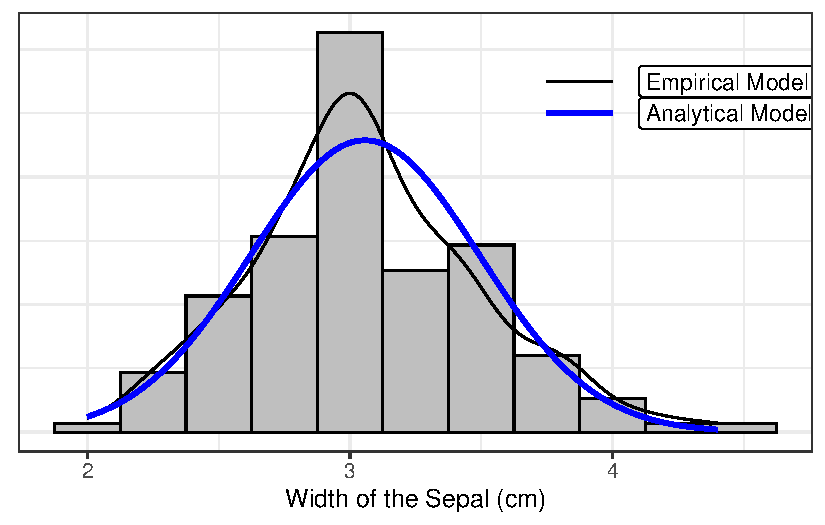
\includegraphics[width=0.8\textwidth,height=\textheight]{./images/fig-regconditions-iris-normal-1.pdf}

}

\caption{\label{fig-regconditions-iris-normal}Summary of the
distribution of the sepal widths for a sample of irises with an
analytical model of the distribution overlayed.}

\end{figure}%

A density (whether constructed empirically or posited analytically) is
just a model for the distribution of a variable. Further, all density
functions share a few basic properties:

\begin{enumerate}
\def\labelenumi{\arabic{enumi}.}
\tightlist
\item
  The density is non-negative for all values of the variable.
\item
  The area under the density function must equal 1.
\end{enumerate}

While the value on the y-axis is not directly meaningful, density
functions provide a link between the value of the variable and the
likelihood of it occurring. Specifically, the probability that a
variable falls in a specific range corresponds to the area under the
curve in that region. For example, based on the analytical model
described above (the blue curve in
Figure~\ref{fig-regconditions-iris-normal}), the probability that an
iris has a sepal width between 3.5 and 4 centimeters is 0.14,
illustrated in Figure~\ref{fig-regconditions-iris-prob}. That is, there
is a 14\% chance a randomly selected iris will have a sepal width
between 3.5 and 4 centimeters based on this model.

\begin{figure}

\centering{

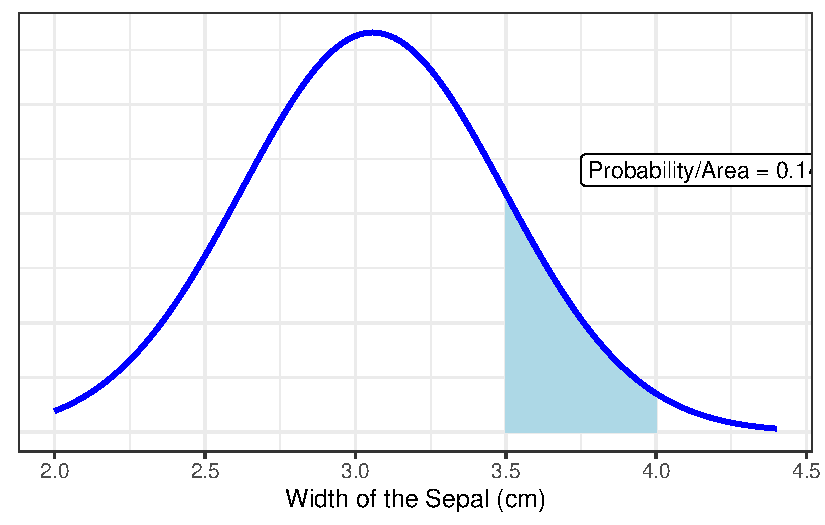
\includegraphics[width=0.8\textwidth,height=\textheight]{./images/fig-regconditions-iris-prob-1.pdf}

}

\caption{\label{fig-regconditions-iris-prob}Using the model for a
density function to compute a probability.}

\end{figure}%

While the above model for the population is not a perfect fit to the
data, it does capture many of the characteristics present in the sample.
Similar to empirical models, analytical models for distributions are
just that --- \emph{models}. As stated previously, the term
``analytical'' does not mean the model does not rely on the data. It is
the \emph{form} of the model that is predetermined; specific components
of the model were estimated based on the available data. The particular
model illustrated in Figure~\ref{fig-regconditions-iris-normal},
characterized by the bell-shape density, is known as the \textbf{Normal
Distribution}.

\begin{definition}[Normal
Distribution]\protect\hypertarget{def-normal-distribution}{}\label{def-normal-distribution}

Also called the Gaussian Distribution, this probability model is popular
for modeling noise within a data generating process. It has the
following characteristics:

\begin{itemize}
\tightlist
\item
  It is bell-shaped.
\item
  It is symmetric, meaning the mean is directly at its center, and the
  lower half of the distribution looks like a mirror image of the upper
  half of the distribution.
\item
  Often useful for modeling noise due to natural phenomena or sums of
  measurements.
\end{itemize}

The functional form of the Normal distribution is

\[f(x) = \frac{1}{\sqrt{2\pi\sigma^2}} e^{-\frac{1}{2\sigma^2}(x - \mu)^2}\]

where \(\mu\) is the mean of the distribution and \(\sigma^2\) is the
variance of the distribution.

\end{definition}

While there are several nice properties of the Normal Distribution, we
are primarily interested in the fact that if the error in a data
generating process follows a Normal Distribution (in addition to the
other three conditions described above placed on the error term), then
the form of the sampling distribution for the least squares estimates of
the slope and intercept is known. That is, with all four conditions in
place, we have an analytical model for the sampling distribution. This
means we avoid simulating in order to build a model for the sampling
distribution; so, computationally it is faster. If the errors really are
from a Normal Distribution, then we also gain power in our study by
imposing this condition.

\begin{tcolorbox}[enhanced jigsaw, breakable, titlerule=0mm, colframe=quarto-callout-note-color-frame, bottomtitle=1mm, opacityback=0, rightrule=.15mm, toptitle=1mm, arc=.35mm, bottomrule=.15mm, left=2mm, title=\textcolor{quarto-callout-note-color}{\faInfo}\hspace{0.5em}{Normality}, leftrule=.75mm, coltitle=black, toprule=.15mm, colbacktitle=quarto-callout-note-color!10!white, colback=white, opacitybacktitle=0.6]

The normality condition states that the distribution of the errors
follows the functional form of a Normal distribution
(Definition~\ref{def-normal-distribution}).

\end{tcolorbox}

\begin{tcolorbox}[enhanced jigsaw, breakable, titlerule=0mm, colframe=quarto-callout-tip-color-frame, bottomtitle=1mm, opacityback=0, rightrule=.15mm, toptitle=1mm, arc=.35mm, bottomrule=.15mm, left=2mm, title=\textcolor{quarto-callout-tip-color}{\faLightbulb}\hspace{0.5em}{Big Idea}, leftrule=.75mm, coltitle=black, toprule=.15mm, colbacktitle=quarto-callout-tip-color!10!white, colback=white, opacitybacktitle=0.6]

If we are willing to assume the distribution of the errors in
Equation~\ref{eq-slr} follows a Normal distribution, then we have an
analytical model for the sampling distribution of the least squares
estimates.

\end{tcolorbox}

Let's think about what this condition means for the responses. Given the
shape of the Normal distribution, imposing this condition (in addition
to the other conditions) implies that some errors are positive and some
are negative. This in turn implies that some responses will tend to fall
above the line (we will under-predict for these observations), and some
response will tend to fall below the line (we will over-predict for
these observations).

\section{Classical Regression Model}\label{classical-regression-model}

We have discussed four conditions we could place on the stochastic
portion of the data generating process. Placing all four conditions on
the error term is what we refer to as the ``Classical Regression
Model.''

\begin{definition}[Classical Regression
Model]\protect\hypertarget{def-classical-regression}{}\label{def-classical-regression}

For a quantitative response and single predictor, the classical
regression model assumes the following data generating process:

\[(\text{Response})_i = \beta_0 + \beta_1 (\text{Predictor})_{i} + \epsilon_i\]

where

\begin{enumerate}
\def\labelenumi{\arabic{enumi}.}
\tightlist
\item
  The error in the response has a mean of 0 for all values of the
  predictor.
\item
  The error in the response for one subject is independent of the error
  in the response for all other subjects.
\item
  The variability in the error of the response is the same for all
  values of the predictor.
\item
  The errors follow a Normal Distribution.
\end{enumerate}

This is the default ``regression'' analysis implemented in the majority
of statistical packages.

\end{definition}

\begin{tcolorbox}[enhanced jigsaw, breakable, titlerule=0mm, colframe=quarto-callout-warning-color-frame, bottomtitle=1mm, opacityback=0, rightrule=.15mm, toptitle=1mm, arc=.35mm, bottomrule=.15mm, left=2mm, title=\textcolor{quarto-callout-warning-color}{\faExclamationTriangle}\hspace{0.5em}{Warning}, leftrule=.75mm, coltitle=black, toprule=.15mm, colbacktitle=quarto-callout-warning-color!10!white, colback=white, opacitybacktitle=0.6]

A ``hidden'' (typically unstated but should not be ignored) condition is
that the sample is representative of the underlying population. In the
one sample case (Chapter~\ref{sec-meanmodels}), we referred to this as
the errors being ``identically distributed.'' We no longer use the
``identically distributed'' language for technical reasons; however, we
still require that the sample be representative of the underlying
population.

\end{tcolorbox}

We note that ``regression'' need not require all four conditions imposed
in Definition~\ref{def-classical-regression}. Placing all four
conditions on the error term results in a specific analytical model for
the sampling distribution of the least squares estimates. Changing the
conditions changes the way we model the sampling distribution.

\begin{tcolorbox}[enhanced jigsaw, breakable, titlerule=0mm, colframe=quarto-callout-tip-color-frame, bottomtitle=1mm, opacityback=0, rightrule=.15mm, toptitle=1mm, arc=.35mm, bottomrule=.15mm, left=2mm, title=\textcolor{quarto-callout-tip-color}{\faLightbulb}\hspace{0.5em}{Big Idea}, leftrule=.75mm, coltitle=black, toprule=.15mm, colbacktitle=quarto-callout-tip-color!10!white, colback=white, opacitybacktitle=0.6]

The model for the sampling distribution of a statistic is determined by
the conditions you place on the stochastic portion of the model for the
data generating process.

\end{tcolorbox}

We have stressed the implications of each condition individually.
Figure~\ref{fig-regconditions-assumptions} illustrates these conditions
working together. The mean-0 condition implies that for a given value of
the predictor, the average response is given by the line (shown as the
dark green dot in the figure). The Normality condition implies that for
a given value of the predictor, the response is distributed evenly about
the regression line according to a Normal distribution; further, the
shape of the Normal distribution implies that these responses will
cluster about the line. The constant variance condition implies that
while the responses vary around the line, they do so to the same degree,
regardless of the value of the predictor; therefore, the model is just
as precise for all values of the predictor. Finally, the independence
condition implies the amount one observation deviates from the line is
unrelated to the amount any other observation deviates from the line.

\begin{figure}

\centering{

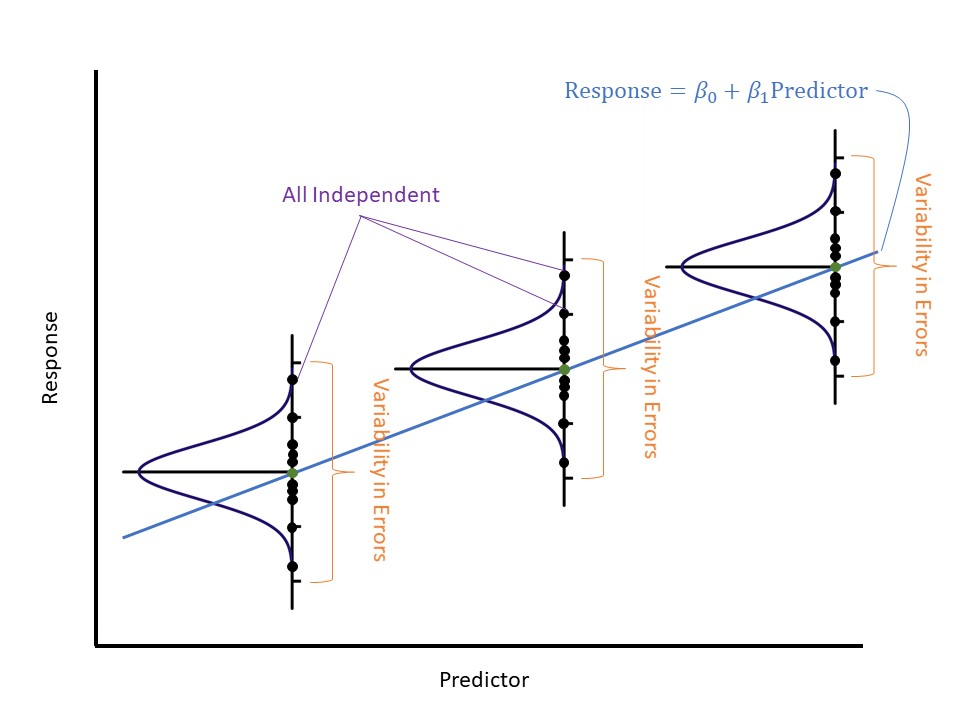
\includegraphics[width=0.8\textwidth,height=\textheight]{./images/RegConditions-Assumptions.jpg}

}

\caption{\label{fig-regconditions-assumptions}Illustration of the
conditions on the error term for the classical regression model.}

\end{figure}%

\section{Imposing the Conditions}\label{imposing-the-conditions}

Let's return to our model for the data generating process of the
bracketed duration as a function of the magnitude of the corresponding
earthquake:

\[(\text{Bracketed Duration})_i = \beta_0 + \beta_1(\text{Magnitude})_i + \varepsilon_i.\]

We were interested in the following research question:

\begin{quote}
On average, are changes in the magnitude of an earthquake associated
with changes in the bracketed duration observed?
\end{quote}

This was captured by the following hypotheses:

\begin{quote}
\(H_0: \beta_1 = 0\)\\
\(H_1: \beta_1 \neq 0\)
\end{quote}

Using the method of least squares, we constructed point estimates of the
parameters in the model; this leads to the following equation for
estimating the average bracketed duration given the magnitude:

\[(\text{Brackted Duration}) = -19.19 + 4.48(\text{Magnitude}).\]

If we are willing to assume the data is consistent with the conditions
for the classical regression model, we are able to model the sampling
distribution (see Appendix~\ref{sec-app-theory}) of these estimates
analytically and therefore construct confidence intervals.
Table~\ref{tbl-regconditions-slr-summary} summarizes the fit for the
above model. In addition to the least squares estimates, it also
contains the standard error (see Definition~\ref{def-standard-error}) of
each statistic, quantifying the variability in the estimates. Finally,
there is a 95\% confidence interval for each parameter. Notice that
based on the confidence interval for the slope, 0 is not a reasonable
value for this parameter. Therefore, we have evidence that the slope
coefficient associated with the magnitude differs from 0; that is, the
sample provides evidence the average bracketed duration depends on the
magnitude of the corresponding earthquake.

\begin{table}

\caption{\label{tbl-regconditions-slr-summary}Summary of the linear
model fit relating the bracketed duration at locations in Greece
following an earthquake with the magnitude of the event.}

\centering{

\centering
\begin{tabular}[t]{lrrrr}
\toprule
Term & Estimate & Standard Error & Lower 95\% CI & Upper 95\% CI\\
\midrule
\cellcolor{gray!10}{(Intercept)} & \cellcolor{gray!10}{-19.194} & \cellcolor{gray!10}{3.975} & \cellcolor{gray!10}{-27.066} & \cellcolor{gray!10}{-11.323}\\
Magnitude & 4.484 & 0.724 & 3.050 & 5.917\\
\bottomrule
\end{tabular}

}

\end{table}%

Chapter~\ref{sec-samplingdistns} described, in general, how confidence
intervals are constructed. Under the classical regression model, there
is an analytical model for the sampling distribution, and it is known.
As a result, the confidence interval can be computed from a formula.

\begin{tcolorbox}[enhanced jigsaw, breakable, titlerule=0mm, colframe=quarto-callout-note-color-frame, bottomtitle=1mm, opacityback=0, rightrule=.15mm, toptitle=1mm, arc=.35mm, bottomrule=.15mm, left=2mm, title=\textcolor{quarto-callout-note-color}{\faInfo}\hspace{0.5em}{Formula for Confidence Interval Under Classical Regression Model}, leftrule=.75mm, coltitle=black, toprule=.15mm, colbacktitle=quarto-callout-note-color!10!white, colback=white, opacitybacktitle=0.6]

If the classical regression model is assumed, the 95\% confidence
interval for the parameter \(\beta_j\) can be approximated by

\[\widehat{\beta}_j \pm (1.96)\left(\text{standard error of } \widehat{\beta}_j\right)\]

\end{tcolorbox}

The confidence interval for the change in the average bracketed duration
for each 1-unit increase in the magnitude of an earthquake (the slope
\(\beta_1\)) was constructed assuming the classical regression model.
Suppose, however, that we are only willing to impose the following
conditions:

\begin{itemize}
\tightlist
\item
  The error in the bracketed duration is 0, on average, for earthquakes
  of any magnitude.
\item
  The error in the bracketed duration for one earthquake is independent
  of the error in the bracketed duration for any other earthquake.
\end{itemize}

Since the conditions for the model of the data generating process have
been altered, the model for the sampling distribution of the estimates
will change, and therefore the corresponding confidence intervals will
also change. Under these reduced conditions, we can appeal to a
bootstrapping algorithm. Specifically, we could resample (with
replacement) 119 earthquakes from the original data; for each resample,
we compute the least squares fit
(Figure~\ref{fig-regconditions-bootstrap}). Since the observations
selected change with each resample, the least squares estimates will
also change. By repeating this process over and over again, we can
obtain a model for how the estimates would change in repeated sampling.

\begin{figure}

\centering{

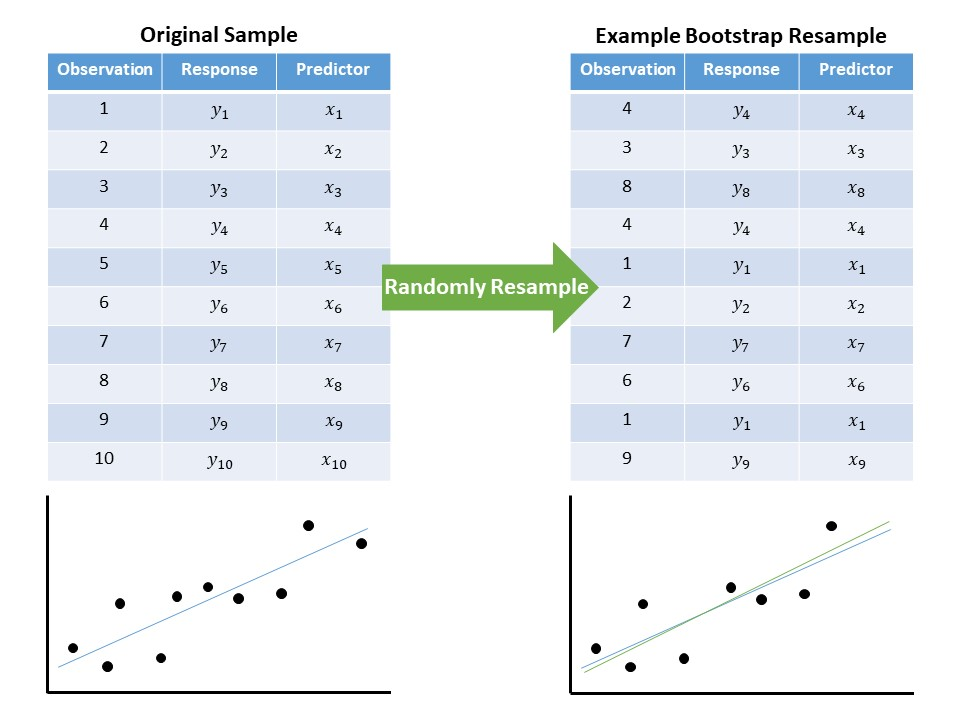
\includegraphics[width=0.8\textwidth,height=\textheight]{./images/RegConditions-Bootstrap.jpg}

}

\caption{\label{fig-regconditions-bootstrap}Illustration of a single
iteration of a bootstrap procedure to construct an empirical estimate of
the sampling distribution for the estimates of the coefficients in a
regression model.}

\end{figure}%

Using the empirical model of the sampling distribution for each
estimate, we can construct a confidence interval for each parameter.
These updated confidence intervals are shown in
Table~\ref{tbl-regconditions-slr-summary-alt}.

\begin{table}

\caption{\label{tbl-regconditions-slr-summary-alt}Summary of the linear
model fit relating the bracketed duration at locations in Greece
following an earthquake with the magnitude of the event. This summary
only assumes the mean-0 and independence conditions.}

\centering{

\centering
\begin{tabular}[t]{lrrrr}
\toprule
Term & Estimate & Standard Error & Lower 95\% CI & Upper 95\% CI\\
\midrule
\cellcolor{gray!10}{(Intercept)} & \cellcolor{gray!10}{-19.194} & \cellcolor{gray!10}{4.960} & \cellcolor{gray!10}{-29.258} & \cellcolor{gray!10}{-9.545}\\
Magnitude & 4.484 & 0.965 & 2.593 & 6.437\\
\bottomrule
\end{tabular}

}

\end{table}%

While the exact interval differs from what we computed previously, our
overall conclusion remains the same --- the sample provides evidence
that the average bracketed duration depends on the magnitude of the
corresponding earthquake. It is natural to ask, which confidence
interval should we use? That depends on the conditions you are willing
to assume, which is an issue we will tackle in
Chapter~\ref{sec-regassessment}.

\section{Recap}\label{recap}

We have covered a lot of ground in this chapter, and it is worth taking
a moment to summarize the big ideas. In order to construct a model for
the sampling distribution of the least squares estimates, we took a step
back and modeled the data generating process. Such a model consists of
two components: a deterministic component explaining the response as a
function of the predictor, and a stochastic component capturing the
noise in the system.

Certain conditions are placed on the distribution of the noise in our
model. With a full set of conditions (classical regression model), we
are able to model the sampling distribution of the least squares
estimates analytically. We can also construct an empirical model for the
sampling distribution of the least squares estimates assuming the data
is consistent with fewer conditions.

In general, the more conditions we are willing to impose on the
data-generating process, the more tractable the analysis; however, the
most important aspect is that the data come from a process which is
consistent with the conditions we impose, which is discussed in
Chapter~\ref{sec-regassessment}.

\chapter{Quantifying the Quality of a Model Fit}\label{sec-regquality}

In the previous two chapters, we described a model for describing the
data generating process for a quantitative response as a function of a
single quantitative predictor:

\[(\text{Response})_i = \beta_0 + \beta_1 (\text{Predictor})_i + \varepsilon_i\]

Chapter~\ref{sec-regmodel} discussed obtaining estimates of these
unknown parameters using the method of least squares.
Chapter~\ref{sec-regconditions} imposed conditions on the stochastic
portion of the model in order to develop a confidence interval for each
parameter. In this chapter, we turn to performing inference through the
computation of a p-value for a set of hypotheses, and we discuss how to
quantify the quality of our model with regard to its utility in making
predictions. It turns out these two tasks are very much related and are
accomplished through partitioning variability. We will describe what we
mean by partitioning variability and how it is used to derive a measure
for the overall performance of a model and to develop a standardized
statistic for comparing two models. As with previous discussions, these
ideas will form another thread of the story that continues throughout
the text.

\section{Partitioning Variability}\label{partitioning-variability}

Let's return to the Seismic Activity Case Study first introduced in
Chapter~\ref{sec-casegreece}. Consider modeling the bracketed duration
at a location as a function of the distance the location is from the
center of the earthquake using the following model for the data
generating process:

\[(\text{Bracketed Duration})_i = \beta_0 + \beta_1(\text{Epicentral Distance})_i + \varepsilon_i.\]

Using least squares to estimate the parameters, and assuming the data is
consistent with the conditions for the classical regression model, the
resulting model fit is summarized below in
Table~\ref{tbl-regquality-fit}.

\begin{table}

\caption{\label{tbl-regquality-fit}Summary of the model fit explaining
the bracketed duration as a function of epicentral distance.}

\centering{

\centering
\begin{tabular}[t]{lrrrr}
\toprule
Term & Estimate & Standard Error & Lower 95\% CI & Upper 95\% CI\\
\midrule
\cellcolor{gray!10}{(Intercept)} & \cellcolor{gray!10}{4.462} & \cellcolor{gray!10}{0.726} & \cellcolor{gray!10}{3.024} & \cellcolor{gray!10}{5.899}\\
Epicentral Distance & 0.029 & 0.018 & -0.007 & 0.064\\
\bottomrule
\end{tabular}

}

\end{table}%

Remember, the goal of the model for the data generating process is to
explain why the response is the value we see --- we are essentially
explaining why the values of the response differ from one individual
unit to another (the variability in the response). Consider the model
for the data generating process summarized above; it includes two
reasons why the bracketed duration is not the same value at each
measured location:

\begin{itemize}
\tightlist
\item
  The locations at which the observations are taken are different
  distances from the epicenter of each earthquake.
\item
  Additional noise due to measurement error in the bracketed duration or
  additional natural sources we are unable to explain or did not account
  for in the model.
\end{itemize}

Looking at the form of the model for the data generating process, it may
seem obvious that there are these two sources of variability --- two
sources for why the bracketed duration differs from one individual
observation to another. Our next endeavor is to quantify the amount of
variability in the response that can be attributed to each of these
components. That is, we move forward with a goal of trying to say
something like

\[\begin{pmatrix} \text{Total Variability} \\ \text{in the Bracketed Duration} \end{pmatrix} = \begin{pmatrix} \text{Variability due} \\ \text{to Distance} \end{pmatrix} + \begin{pmatrix} \text{Variability due} \\ \text{to Noise} \end{pmatrix}\]

As we have seen in both Chapter~\ref{sec-summaries} and
Chapter~\ref{sec-teststat}, variability can be quantified through
considering the ``total'' distance the observations are from a common
target (for example, the mean response) where ``distance'' is captured
by squared deviations. That is, the total variability in bracketed
duration can be measured by

\begin{equation}\phantomsection\label{eq-regquality-sst}{\sum_{i=1}^{n} \left[(\text{Bracketed Duration})_i - (\text{Overall Mean Bracketed Duration})\right]^2.}\end{equation}

Notice this quantity is related to, but not equivalent to, the sample
variance. It measures the distance each response is from the sample mean
and then adds these distances up. This is known as the \textbf{Total Sum
of Squares} since it captures the total variability in the response.

\begin{definition}[Total Sum of
Squares]\protect\hypertarget{def-sst}{}\label{def-sst}

The Total Sum of Squares, abbreviated SST, is given by

\[SST = \sum_{i=1}^{n} \left[(\text{Response})_i - (\text{Overall Mean Response})\right]^2\]

where the overall average response is the sample mean.

\end{definition}

We now have a way of quantifying the total variability in the bracketed
duration; we now want to partition (or separate) out this variability
into its two components: the variability due to the epicentral distance,
and the variability due to noise. In order to capture the variability
due to epicentral distance, we consider how epicentral distance plays a
role in the model for the data generating process: it forms the line
which dictates the mean response. That is, the linear portion in the
model for the data generating process
\(\beta_0 + \beta_1 (\text{Epicentral Distance})\) is the model's
attempt to explain how changes in the epicentral distance explain
changes in the bracketed duration; further, this explanation comes in
the form of the average response. That is, plugging into the
deterministic portion of the model for the data generating process
provides a mean response, and if we use the least squares estimates in
place of the parameters, we are computing an estimate of the mean
response. Finding the variability in the bracketed duration due to the
epicentral distance is then equivalent to finding the variability in
these estimated (or predicted) mean responses:

\begin{equation}\phantomsection\label{eq-regquality-ssr}{\sum_{i=1}^{n} \left[(\text{Predicted Bracketed Duration})_i - (\text{Overall Mean Bracketed Duration})\right]^2.}\end{equation}

This is known as the \textbf{Regression Sum of Squares} as it captures
the variability explained by the regression line.

\begin{definition}[Regression Sum of
Squares]\protect\hypertarget{def-ssr}{}\label{def-ssr}

The Regression Sum of Squares, abbreviated SSR, is given by

\[SSR = \sum_{i=1}^{n} \left[(\text{Predicted Mean Response})_i - (\text{Overall Mean Response})\right]^2\]

where the predicted mean response is computed using the least squares
estimates and the overall mean response is the sample mean.

\end{definition}

Finally, the unexplained noise, \(\varepsilon\) in our model for the
data generating process, is the difference between the actual response
and the deterministic portion of the model (in our case, the true
regression line). This variability in the noise is then the variability
in the bracketed duration where the average is \emph{conditional} on the
epicentral distance instead of ignoring it (which is what happens when
we use the overall sample mean bracketed duration):

\begin{equation}\phantomsection\label{eq-regquality-sse}{\sum_{i=1}^{n} \left[(\text{Bracketed Duration})_i - (\text{Predicted Bracketed Duration})_i\right]^2.}\end{equation}

This is known as the \textbf{Error Sum of Squares} as it captures the
variability not explained by the model but represented by the error term
in the model.

\begin{definition}[Error Sum of
Squares]\protect\hypertarget{def-sse}{}\label{def-sse}

The Error Sum of Squares, abbreviated SSE and sometimes referred to as
the Residual Sum of Squares, is given by

\[SSE = \sum_{i=1}^{n} \left[(\text{Response})_i - (\text{Predicted Mean Response})_i\right]^2\]

where the predicted mean response is computed using the least squares
estimates.

\end{definition}

With some clever algebra, it can be easily seen that the total
variability does in fact partition into these two components. This
discussion is represented in
Figure~\ref{fig-regquality-partition-variability}.

\begin{tcolorbox}[enhanced jigsaw, breakable, titlerule=0mm, colframe=quarto-callout-tip-color-frame, bottomtitle=1mm, opacityback=0, rightrule=.15mm, toptitle=1mm, arc=.35mm, bottomrule=.15mm, left=2mm, title=\textcolor{quarto-callout-tip-color}{\faLightbulb}\hspace{0.5em}{Big Idea}, leftrule=.75mm, coltitle=black, toprule=.15mm, colbacktitle=quarto-callout-tip-color!10!white, colback=white, opacitybacktitle=0.6]

The total variability in a response can be partitioned into two
components: the variability explained by the predictor and the
unexplained variability left in the error term. This is represented in
the formula

\[SST = SSR + SSE\]

\end{tcolorbox}

\begin{figure}

\centering{

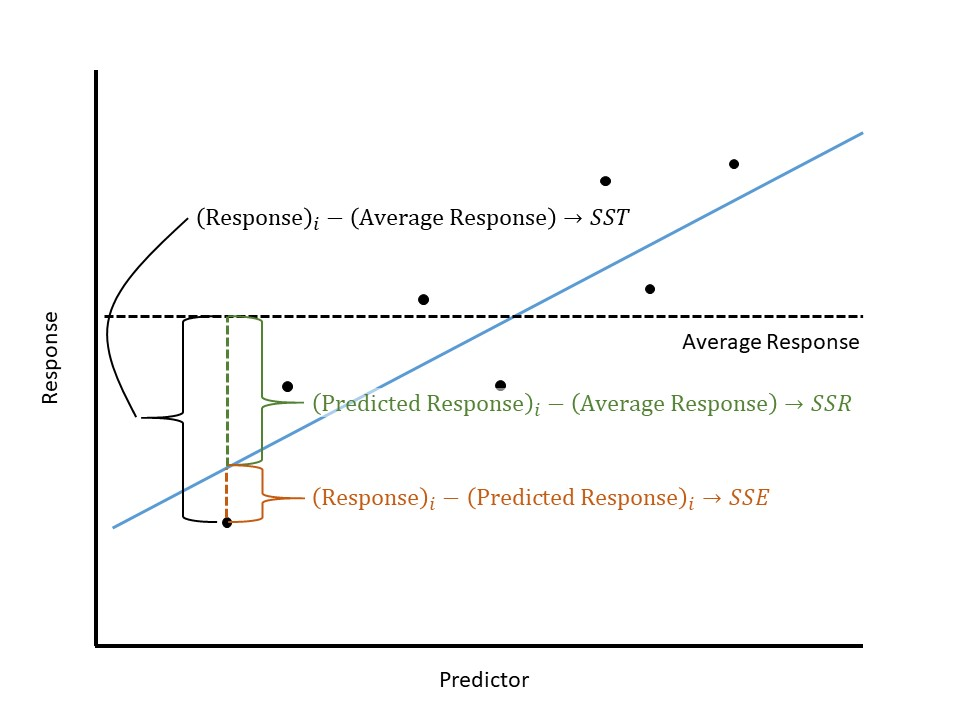
\includegraphics[width=0.8\textwidth,height=\textheight]{./images/RegQuality-Partitioning-Variability.jpg}

}

\caption{\label{fig-regquality-partition-variability}Illustration of
partitioning the variability of a response using a regression model.}

\end{figure}%

\section{R-squared}\label{r-squared}

The key to quantifying the quality of a model for the data generating
process is to understand that a partition breaks a whole into smaller,
distinct components. This means that if you put the components back
together, you have the whole. The sums of squares partition the
variability in the response into that explained by the deterministic
portion of the model for the data generating process and that not
explained. We represented this above by the equation

\[SST = SSR + SSE\].

The benefit partitioning variability is that it makes clear the
breakdown between the variability in the response that the deterministic
portion of the model is explaining (SSR) versus the variability in the
response that cannot be explained (SSE). We are now in a position to
quantify the proportion of the total variability the model is
explaining, which is known as the \textbf{R-squared} value for the
model.

\begin{definition}[R-Squared]\protect\hypertarget{def-r-squared}{}\label{def-r-squared}

Sometimes reported as a percentage, the R-Squared value measures the
proportion of the variability in the response explained by a model. It
is given by

\[\text{R-squared} = \frac{SSR}{SST}.\]

\end{definition}

For our model of the bracketed duration as a function of the epicentral
distance, the R-squared value turns out to be 0.0216; that is, only
2.16\% of the variability in the bracketed duration at a location is
explained by its distance from the center of the corresponding
earthquake.

As R-squared is a proportion, it must take a value between 0 and 1. If
0, that means our model has no predictive ability within our sample.
That is, knowing the predictor does not add to our ability to predict
the response any more than guessing. A value of 1 indicates that our
model has predicted all the variability in the response; that is, given
the predictor, we can perfectly predict the value of the response.

It may appear that obtaining an R-squared value of 1 should be our goal.
And, in one sense, it is. We want a model that has strong predictive
ability. However, there is a danger in obtaining an R-squared of 1 as
well. We must remember that variability is inherent in any process.
Therefore, we should never expect to fully explain all the variability
in a response. George Box (a renowned statistician) once made the
following statement (Box 1979):

\begin{quote}
``Now it would be very remarkable if any system existing in the real
world could be exactly represented by any simple model. However,
cunningly chosen parsimonious models often do provide remarkably useful
approximations. For example, the law \(PV = RT\) relating pressure
\(P\), volume \(V\) and temperature \(T\) of an `ideal' gas via a
constant \(R\) is not exactly true for any real gas, but it frequently
provides a useful approximation and furthermore its structure is
informative since it springs from a physical view of the behavior of gas
molecules.

For such a model there is no need to ask the question `Is the model
true?'. If `truth' is to be the `whole truth' the answer must be `No.'
The only question of interest is `Is the model illuminating and
useful?'.
\end{quote}

The idea here is that we know the model will not capture the data
generating process precisely. Therefore, we should be skeptical of
models which claim to be perfect. For example, consider the two models
illustrated in Figure~\ref{fig-regquality-overfit}. The model
represented by the black line has a perfect fit, but we argue the model
represented by the blue line is better. While the black line captures
all the variability in the response for this sample, it is certainly
trying to do too much. In reality, the blue line captures the underlying
relationship while not overcomplicating that relationship. We sacrifice
a little quality in the fit for \emph{this sample} in order to better
represent the underlying structure of \emph{the population}. The black
line suffers from what is known as \emph{overfitting}; the blue line is
a more \emph{parsimonious} (simple) model, balancing complexity with
model fit.

\begin{figure}

\centering{

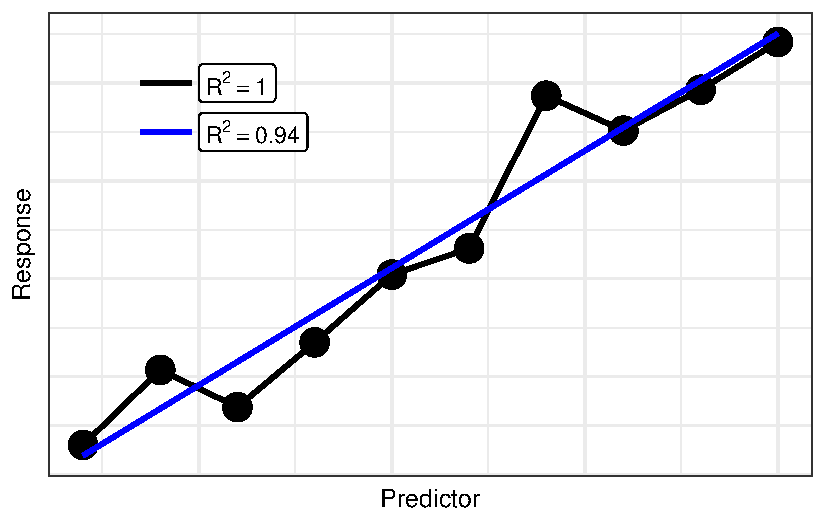
\includegraphics[width=0.8\textwidth,height=\textheight]{./images/fig-regquality-overfit-1.pdf}

}

\caption{\label{fig-regquality-overfit}Illustration of a parsimonious
model compared to one which overfits the data.}

\end{figure}%

Students often ask, ``if not 1, how high of an R-squared represents a
\emph{good} model?'' The answer depends a lot on the discipline. In many
engineering applications within a lab setting, we can control much of
the external variability leading to extremely high R-squared values
(0.95 to 0.99). However, in biological applications, the variability
among the population can be quite large, leading to much smaller
R-squared values (0.3 to 0.6). What is considered ``good'' can depend on
the specific application.

\begin{tcolorbox}[enhanced jigsaw, breakable, titlerule=0mm, colframe=quarto-callout-warning-color-frame, bottomtitle=1mm, opacityback=0, rightrule=.15mm, toptitle=1mm, arc=.35mm, bottomrule=.15mm, left=2mm, title=\textcolor{quarto-callout-warning-color}{\faExclamationTriangle}\hspace{0.5em}{Warning}, leftrule=.75mm, coltitle=black, toprule=.15mm, colbacktitle=quarto-callout-warning-color!10!white, colback=white, opacitybacktitle=0.6]

While R-squared is useful for quantifying the quality of a model on a
set of data, it should not be used to compare two different models as
R-squared always favors more complex models. There are better methods
which adjust for the complexity of the model fit.

\end{tcolorbox}

In addition to the discipline, how you view the R-squared value for a
model may depend on the goal of the model. There are generally two broad
reasons for developing a statistical model:

\begin{itemize}
\tightlist
\item
  Explain the relationship between a response and one or more
  predictors. This can involve examining the marginal relationship,
  isolating the effect, or examining the interplay between predictors.\\
\item
  Predict a future response given a specific value for the predictors.
\end{itemize}

If all we are interested in doing is explaining the relationship, we may
not be concerned about the predictive ability of the model. That is,
since our goal is not to accurately predict a future response, we are
primary concerned with whether we have evidence of a relationship. But,
if our goal is prediction, we would like that estimate to be precise. In
such cases, a high R-squared is required before really relying on the
model we have.

What is perhaps counter-intuitive is that, while related, hypothesis
testing and the R-squared value may not necessarily yield the same
conclusions. That is, it is possible that we have a strong evidence that
the average response depends on the predictor (small p-value) \emph{and}
simultaneously conclude that using the predictor would not result in
precise predictions (low R-squared value).

\section{Hypothesis Testing}\label{hypothesis-testing-1}

In addition to quantifying the quality of the model, partitioning the
variability in a response into two components is the basis for
conducting a hypothesis test to compare two models. In this section, we
expand upon the ideas initially presented in Chapter~\ref{sec-teststat},
broadening them to add to our unifying framework. Recall that hypothesis
testing is really about comparing two models for the data generating
process: a more complex model in which the parameters are free to take
on any value, and a restricted model in which the parameters are
constrained in some way.

When the sample does not provide enough evidence to suggest the more
complex model is necessary to explain the variability in the response,
we conclude it is reasonable the reduced model for the data generating
process is appropriate (some say, we ``fail to reject'' the null
hypothesis). When the sample does provide sufficient evidence to suggest
we can discern the difference in the performance of the reduced and
complex model, we say the simple model is not sufficient for explaining
the variability in the response, and we prefer the more complex model
(some say, we ``reject'' the null hypothesis). Throughout the remainder
of this section, we will consider the following research question:

\begin{quote}
Is there evidence the average bracketed duration for a location
following an earthquake is linearly related to the distance the location
is from the center of the earthquake?
\end{quote}

If we consider the simple linear model for the data generating process
described above, this question can be captured using the following set
of hypotheses:

\[H_0: \beta_1 = 0 \qquad \text{vs.} \qquad H_1: \beta_1 \neq 0.\]

Again, hypothesis testing is really model comparison; that is, these
hypotheses are really suggesting two separate models for the data
generating process:

\[
\begin{aligned}
  \text{Model 1}:& \quad (\text{Bracketed Duration})_i = \beta_0 + \beta_1 (\text{Epicentral Distance})_i + \varepsilon_i \\
  \text{Model 0}:& \quad (\text{Bracketed Duration})_i = \beta_0 + \varepsilon_i.
\end{aligned}
\]

The model under the null hypothesis (Model 0) has fewer parameters
because it is a constrained version of Model 1 resulting from setting
\(\beta_1 = 0\). In fact, while Model 1 says that there are two
components (the epicentral distance and noise) contributing to the
variability observed in the bracketed duration, Model 0 says that there
is only a single component (noise). So, we can think of our hypotheses
as

\[
\begin{aligned}
  H_0: \text{Model 0 is sufficient for explaining the variability in the response} \\
  H_1: \text{Model 0 is not sufficient for explaining the variability in the response.}
\end{aligned}
\]

Regardless of which model we choose, the total variability in the
response remains the same. We are simply asking whether the variability
explained by the predictor is sufficiently large for us to say it has an
impact. In particular, if the null hypothesis were true, we would expect
all the variability in the response to be channeled into the noise
(\(SST \approx SSE\)). In fact, think about computing the error sum of
squares for Model 0 above; it would be

\[SSE_0 = \sum_{i=1}^{n} \left[(\text{Bracketed Duration})_i - (\text{Overall Average Bracketed Duration})\right]^2\]

since the least squares estimate of \(\widehat{\beta}_0\) in Model 0 is
the sample mean (see Appendix~\ref{sec-app-teststat}). But, this is
equivalent to the total sum of squares for Model 1
(Equation~\ref{eq-regquality-sst}). This confirms our intuition that if
the null hypothesis were true, we would expect all the variability in
the response to be channeled into the noise (\(SST \approx SSE\)).

If, however, the alternative hypothesis is true and the epicentral
distance explains some portion of the variability in the bracketed
duration, then we would expect some of the variability to be channeled
out of the noise term (\(SSR > 0\)). Because we have partitioned the
variability, we now take a moment to recognize that

\[SSR = SST - SSE,\]

but we know that the total sum of squares is just the error sum of
squares from the reduced model (Model 0) as shown above. Therefore, we
can write

\begin{equation}\phantomsection\label{eq-regquality-ssr-difference}{SSR = SSE_0 - SSE_1,}\end{equation}

where we use the subscripts to denote whether we are discussing the
error sum of squares from the reduced model (Model 0) or the full
unconstrained model (Model 1). That is,
Equation~\ref{eq-regquality-ssr-difference} reveals that the regression
sum of squares is the equivalent of the shift in the error sum of
squares as we move from the reduced model under the null hypothesis to
the more complex model under the alternative hypothesis.

\begin{tcolorbox}[enhanced jigsaw, breakable, titlerule=0mm, colframe=quarto-callout-tip-color-frame, bottomtitle=1mm, opacityback=0, rightrule=.15mm, toptitle=1mm, arc=.35mm, bottomrule=.15mm, left=2mm, title=\textcolor{quarto-callout-tip-color}{\faLightbulb}\hspace{0.5em}{Big Idea}, leftrule=.75mm, coltitle=black, toprule=.15mm, colbacktitle=quarto-callout-tip-color!10!white, colback=white, opacitybacktitle=0.6]

For a particular dataset, the regression sum of squares quantifies the
shift in the error sum of squares as we move from a reduced model to a
more complex model. It measures the ``signal'' in the data represented
by the more complex model for the data generating process.

\end{tcolorbox}

The regression sum of squares represents our signal. The larger the
value, the more evidence we have that the data is not consistent with
the null hypothesis. However, as we saw in Chapter~\ref{sec-teststat},
we should always examine our signal relative to the noise in the data.
We already have a measure for the amount of variability due to noise ---
the error sum of squares! It then seems reasonable to consider the ratio

\[\frac{SSR}{SSE_1} = \frac{SST - SSE_1}{SSE_1} = \frac{SSE_0 - SSE_1}{SSE_1},\]

where again we have added subscripts to emphasize from which model we
are computing the sums of squares. While this is a reasonable statistic,
it is not yet standardized. Remember that sums of squares capture
variability but are themselves not variances, and it turns out a ratio
of variances is easier to model analytically. If we take a sum of
squares and divide by an appropriate term, known as the \textbf{degrees
of freedom}, we get a true variance term.

\begin{definition}[Degrees of
Freedom]\protect\hypertarget{def-df}{}\label{def-df}

A measure of the flexibility in a sum of squares term; when a sum of
squares is divided by the corresponding degrees of freedom, the result
is a variance term.

\end{definition}

\begin{tcolorbox}[enhanced jigsaw, breakable, titlerule=0mm, colframe=quarto-callout-note-color-frame, bottomtitle=1mm, opacityback=0, rightrule=.15mm, toptitle=1mm, arc=.35mm, bottomrule=.15mm, left=2mm, title=\textcolor{quarto-callout-note-color}{\faInfo}\hspace{0.5em}{Rationale for Degrees of Freedom}, leftrule=.75mm, coltitle=black, toprule=.15mm, colbacktitle=quarto-callout-note-color!10!white, colback=white, opacitybacktitle=0.6]

Degrees of freedom are a very difficult concept to grasp, even for those
who have been studying statistics for a while. Here is our way of
thinking about them --- they are the difference of available terms to
work with. For example, think about the total sum of squares associated
with a full unconstrained linear regression model described in
Equation~\ref{eq-slr}:

\[SST = \sum_{i=1}^{n} \left[(\text{Response})_i - (\text{Overall Mean Response})\right]^2.\]

The first term of the difference has \(n\) different values (one
response for each observation). However, the sample mean is just one
value. Therefore, there are \(n - 1\) degrees of freedom associated with
the total sum of squares. This is often described as starting out with
\(n\) estimates (the data), but needing to estimate one parameter (the
mean) along the way, leading to \(n - 1\).

Similarly, consider the regression sum of squares for the full
unconstrained model:

\[SSR = \sum_{i=1}^{n} \left[(\text{Predicted Mean Response})_i - (\text{Overall Mean Response})\right]^2.\]

While there are \(n\) predicted values, they are all generated from the
same least squares fit
\(\widehat{\beta}_0 + \widehat{\beta}_1 (\text{Predictor})_i\) which can
be computed from two estimates (that for the intercept and slope).
Therefore, we begin with only 2 unique values. Again, the sample mean
has just one value, leading to \(2 - 1 = 1\) degree of freedom
associated with the regression sum of squares.

Finally, consider the error sum of squares for the full unconstrained
model:

\[SSE = \sum_{i=1}^{n} \left[(\text{Response})_i - (\text{Predicted Mean Response})_i\right]^2.\]

We have \(n\) initial values (one for each observation). However, as
described above, we only need 2 terms to estimate the predicted values.
So, we have \(n - 2\) degrees of freedom associated with the error sum
of squares.

Note that just as the sums of squares formed a partition
(\(SST = SSR + SSE\)), the corresponding degrees of freedom form a
partition (\((n - 1) = (2 - 1) + (n - 2)\)).

\end{tcolorbox}

Again, dividing a sum of squares by its associated degrees of freedom
creates a variance term; this term is known as a \textbf{mean square}.
It is important to note that both sums of squares and mean squares
quantify the components of variability in the response, the component
explained by the deterministic portion of the model and the component
that is unexplained. However, they serve different purposes.

\begin{definition}[Mean
Square]\protect\hypertarget{def-ms}{}\label{def-ms}

A mean square is the ratio of a sum of squares and its corresponding
degrees of freedom. For a model of the form in Equation~\ref{eq-slr}, we
have

\begin{itemize}
\tightlist
\item
  \textbf{Mean Square Total (MST)}: estimated variance of the responses;
  this is the same as the sample variance of the response.
\item
  \textbf{Mean Square for Regression (MSR)}: estimated variance of the
  predicted responses.
\item
  \textbf{Mean Square Error (MSE)}: estimated variance of the error
  terms; this is equivalent to the estimated variance of the response
  for a given value of the predictor (the variance of the response about
  the regression line).
\end{itemize}

In each case, the mean square is an estimated variance.

\end{definition}

\begin{tcolorbox}[enhanced jigsaw, breakable, titlerule=0mm, colframe=quarto-callout-note-color-frame, bottomtitle=1mm, opacityback=0, rightrule=.15mm, toptitle=1mm, arc=.35mm, bottomrule=.15mm, left=2mm, title=\textcolor{quarto-callout-note-color}{\faInfo}\hspace{0.5em}{Note}, leftrule=.75mm, coltitle=black, toprule=.15mm, colbacktitle=quarto-callout-note-color!10!white, colback=white, opacitybacktitle=0.6]

Sums of squares partition the variability of the response into smaller
components; mean squares estimate the variance of those smaller
components. While \(SST = SSR + SSE\), note that \(MST \neq MSR + MSE\).

\end{tcolorbox}

Since mean squares are proportional to their corresponding sum of
squares, an increase in the sum of squares is associated with an
increase in the corresponding mean square. We are now ready to define
our standardized statistic as the ratio of mean squares. Instead of the
ratio

\[\frac{SSR}{SSE_1} = \frac{SST - SSE_1}{SSE_1} = \frac{SSE_0 - SSE_1}{SSE_1},\]

we replace the numerator and denominator with mean squares such that

\[\frac{MSR}{MSE} = \frac{\left(SST - SSE_1\right)/(2 - 1)}{SSE_1/(n - 2)} = \frac{\left(SSE_0 - SSE_1\right)/(2 - 1)}{SSE_1/(n - 2)},\]

where again we have added subscripts to emphasize from which model we
are computing the sums of squares. This standardized statistic could be
used to quantify the signal-to-noise ratio (the amount of evidence) in
the sample for testing the hypotheses

\begin{quote}
\(H_0: \beta_1 = 0\)\\
\(H_1: \beta_1 \neq 0.\)
\end{quote}

However, we can generalize this for testing a range of hypotheses within
our model for the data generating process.

\begin{definition}[Standardized Statistic for Simple Linear
Regression]\protect\hypertarget{def-standard-f}{}\label{def-standard-f}

Consider testing a set of hypotheses for a model of the data generating
process of the form (Equation~\ref{eq-slr}):

\[(\text{Response})_i = \beta_0 + \beta_1(\text{Predictor})_i + \varepsilon_i.\]

Denote this model as Model 1, and denote the model that results from
applying the parameter constraints defined under the null hypothesis as
Model 0\footnote{Technically, this standardized statistic only applies
  to a class of potential hypotheses, but that class is quite broad (see
  Appendix~\ref{sec-app-teststat}).}. A standardized statistic,
sometimes called the ``standardized F statistic,'' for testing the
hypotheses is given by

\[T^* = \frac{\left(SSE_0 - SSE_1\right) / (2 - r)}{SSE_1 / (n - 2)},\]

where \(r\) is the number of parameters in the reduced model. Defining

\[MSA = \frac{SSE_0 - SSE_1}{2 - r}\]

to be the ``mean square for additional terms,'' which captures the shift
in the error sum of squares from the reduced model to the full
unconstrained model, we can write the standardized statistic as

\[T^* = \frac{MSA}{MSE}\]

where the mean square error in the denominator comes from the full
unconstrained model.

\end{definition}

It can be shown that this standardized statistic is a generalization of
the one introduced in Chapter~\ref{sec-teststat}. The numerator captures
the signal by examining the difference between what we expect the error
sum of squares to be under the null hypothesis and what we actually
observe; the denominator captures the background noise (relative to the
estimated mean response from the full model). Larger values of this
standardized statistic indicate more evidence in the sample against the
null hypothesis.

We should not lose sight of the fact that our standardized statistic is
really a result of partitioning the variability and considering the
variability explained by the predictor relative to the noise in the
response. Underscoring that the standardized statistic is a result of
this partitioning, the analyses of these sources of variability is often
summarized in a table similar to that represented in
Figure~\ref{fig-regquality-ANOVA-table}.

\begin{figure}

\centering{

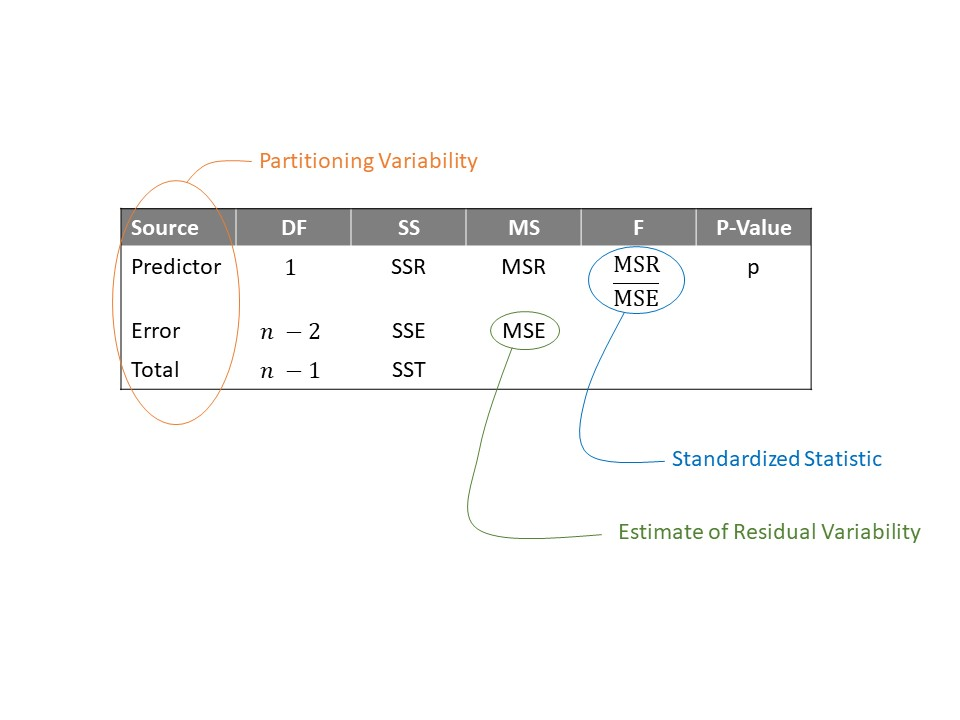
\includegraphics[width=0.8\textwidth,height=\textheight]{./images/RegQuality-ANOVA-Table.jpg}

}

\caption{\label{fig-regquality-ANOVA-table}Table summarizing the
partitioning of variability in a regression model.}

\end{figure}%

The last entry in the table is the p-value. As with any p-value, it is
computed by finding the likelihood, assuming the null hypothesis is
true, of obtaining a standardized statistic, by chance alone, as extreme
or more so than that observed in our sample. ``More extreme'' values of
the statistic would be larger values; so, the area to the right in the
model for the null distribution is needed. The key step is modeling that
null distribution. This is where the conditions we place on the error
term that were discussed in Chapter~\ref{sec-regconditions} come into
play. Under the classical regression conditions, we can model the null
distribution analytically (see Appendix~\ref{sec-app-theory});
otherwise, we can rely on bootstrapping to model the null distribution.

Let's return to our question that inspired our investigation:

\begin{quote}
Is there evidence the average bracketed duration for a location
following an earthquake is linearly related to the distance the location
is from the center of the earthquake?
\end{quote}

This corresponds to testing the hypotheses

\[H_0: \beta_1 = 0 \qquad \text{vs.} \qquad H_1: \beta_1 \neq 0.\]

Table~\ref{tbl-regquality-anova} gives the table summarizing the
partitioned sources of variability in the bracketed duration. We have a
large p-value (computed assuming the data is consistent with the
classical regression model). That is, the sample provides no evidence to
suggest that locations further from the center of the earthquake
experience a bracketed duration which differs, on average, from those
closer to the center of the earthquake.

\begin{table}

\caption{\label{tbl-regquality-anova}Analysis of the sources of
variability in the bracketed duration as a function of epicentral
distance.}

\centering{

\centering\centering
\resizebox{\ifdim\width>\linewidth\linewidth\else\width\fi}{!}{
\begin{tabular}[t]{lrrrrr}
\toprule
Term & DF & Sum of Squares & Mean Square & Standardized Statistic & P-Value\\
\midrule
\cellcolor{gray!10}{\cellcolor{gray!10}{Epicentral Distance}} & \cellcolor{gray!10}{\cellcolor{gray!10}{1}} & \cellcolor{gray!10}{\cellcolor{gray!10}{85.733}} & \cellcolor{gray!10}{\cellcolor{gray!10}{85.733}} & \cellcolor{gray!10}{\cellcolor{gray!10}{2.583}} & \cellcolor{gray!10}{\cellcolor{gray!10}{0.111}}\\
Error & 117 & 3883.708 & 33.194 &  & \\
\bottomrule
\end{tabular}}

}

\end{table}%

\begin{tcolorbox}[enhanced jigsaw, breakable, titlerule=0mm, colframe=quarto-callout-tip-color-frame, bottomtitle=1mm, opacityback=0, rightrule=.15mm, toptitle=1mm, arc=.35mm, bottomrule=.15mm, left=2mm, title=\textcolor{quarto-callout-tip-color}{\faLightbulb}\hspace{0.5em}{Big Idea}, leftrule=.75mm, coltitle=black, toprule=.15mm, colbacktitle=quarto-callout-tip-color!10!white, colback=white, opacitybacktitle=0.6]

Determining if a response is linearly related to a predictor is done by
determining if the predictor explains a significant portion of the
variability in the response.

\end{tcolorbox}

In this section, we partitioned variability as a way of evaluating the
strength of evidence the predictor plays in determining the response. In
the previous section, we used that same partition to quantify the
predictive ability of the model for the data generating process.
Regardless of our goal, conducting inference or predicting a future
response, partitioning the variability is a key step. If inference is
our primary aim, this partitioning allows us to determine if a predictor
adds to the model above and beyond the error alone. If prediction is our
primary aim, the partitioning allows us to quantify the quality of the
model's predictive ability.

\chapter{Assessing the Modeling Conditions}\label{sec-regassessment}

We have been considering the simple linear model described in
Equation~\ref{eq-slr} for the data generating process of a quantitative
response. For example, for the Seismic Activity Case Study, we
considered a model that explained the bracketed duration at a location
as a function of the magnitude of the earthquake:

\[(\text{Bracketed Duration})_i = \beta_0 + \beta_1(\text{Magnitude})_i + \varepsilon_i.\]

Estimates for the unknown parameters in this model were obtained using
the method of least squares (Chapter~\ref{sec-regmodel}). In order to
obtain a model for the sampling distribution of these estimates (or the
null distribution as appropriate), and thereby conduct inference, we
added conditions to the distribution of the error term
(Chapter~\ref{sec-regconditions}). For example, under the ``classical
regression model'' (Definition~\ref{def-classical-regression}) we
require the following four conditions:

\begin{enumerate}
\def\labelenumi{\arabic{enumi}.}
\tightlist
\item
  The error in the bracketed duration has an average of 0 regardless of
  the magnitude of the earthquake.
\item
  The error in the bracketed duration for one location is independent of
  the error in the bracketed duration for any other location.
\item
  The variability of the error in the bracketed duration is the same
  regardless of the magnitude of the earthquake.
\item
  The errors in the bracketed duration follow a Normal distribution.
\end{enumerate}

We also saw in Chapter~\ref{sec-regconditions}, that we could develop an
empirical model for the sampling distribution of the least squares
estimates only enforcing the first two of these conditions on the
distribution of the error. Which of these two models for the sampling
distribution should be used? Unfortunately, we cannot simply state
conditions and then proceed blindly. In order to rely on the p-values
and confidence intervals produced from any modeling procedure, the data
must be consistent with these conditions.

In this section, we discuss how we assess these conditions
qualitatively.

\section{Residuals}\label{residuals}

One of the complications we face is that we are imposing conditions on
the error term, but we do not observe the error (since the parameters
are unknown). However, we are able to determine the difference between
each observation with respect to the \emph{estimated} model for the data
generating process. This difference between each observed response and
what we would have predicted for this observation using the least
squares estimates, called a \textbf{residual}, is analogous to the error
term if the parameters were known. Therefore, residuals should behave
like a sample of error terms.

\begin{definition}[Residual]\protect\hypertarget{def-residual}{}\label{def-residual}

The difference between the observed response and the predicted response
(estimated deterministic portion of the model). Specifically, the
residual for the \(i\)-th observation is given by

\[(\text{Residual})_i = (\text{Response})_i - (\text{Predicted Mean Response})_i\]

where the ``predicted mean response'' is often called the predicted, or
fitted, value.

Residuals mimic the noise in the data generating process.

\end{definition}

For the simple linear regression model, the predicted mean response is
computed by plugging into the formula

\[\widehat{\beta}_0 + \widehat{\beta}_1 (\text{Predictor})_{i},\]

where \(\widehat{\beta}_0\) and \(\widehat{\beta}_1\) are the least
squares estimates. We can use the residuals to qualitatively assess if
the observed data is consistent with each of the four potential
conditions we might place on the distribution of the error term.

\begin{tcolorbox}[enhanced jigsaw, breakable, titlerule=0mm, colframe=quarto-callout-tip-color-frame, bottomtitle=1mm, opacityback=0, rightrule=.15mm, toptitle=1mm, arc=.35mm, bottomrule=.15mm, left=2mm, title=\textcolor{quarto-callout-tip-color}{\faLightbulb}\hspace{0.5em}{Big Idea}, leftrule=.75mm, coltitle=black, toprule=.15mm, colbacktitle=quarto-callout-tip-color!10!white, colback=white, opacitybacktitle=0.6]

Residuals, since they mimic the noise in the data generating process,
provide a way of assessing the modeling conditions placed on the
distribution of the error term. The conditions are placed on the error
term, but they are assessed with residuals.

\end{tcolorbox}

\section{Assessing the Mean-0
Condition}\label{assessing-the-mean-0-condition}

\begin{quote}
The error in the bracketed duration has an average of 0 regardless of
the magnitude of the earthquake.
\end{quote}

It is tempting to read this condition and believe that a rational way to
assess this condition is to determine if the average of the residuals is
0. However, while the difference is subtle, the condition is \emph{not}
that the average error is 0; the condition is that the average error is
0 for \emph{all values of the predictor}. It would seem we need to
determine if, for each value of the predictor possible, if the residuals
average to 0. This is infeasible numerically because we do not generally
have multiple responses for each value of the predictor. We can,
however, assess whether the data is consistent with this condition
graphically. That is, in order to assess this condition, we need to
graphically assess how the average behaves over a range of predictor
values. We capture this by looking at the \emph{predicted (or fitted)
values}. Figure~\ref{fig-regassessment-mean0} shows the relationship
between the residuals and the associated predicted values for the
observations in the data set.

\begin{figure}

\centering{

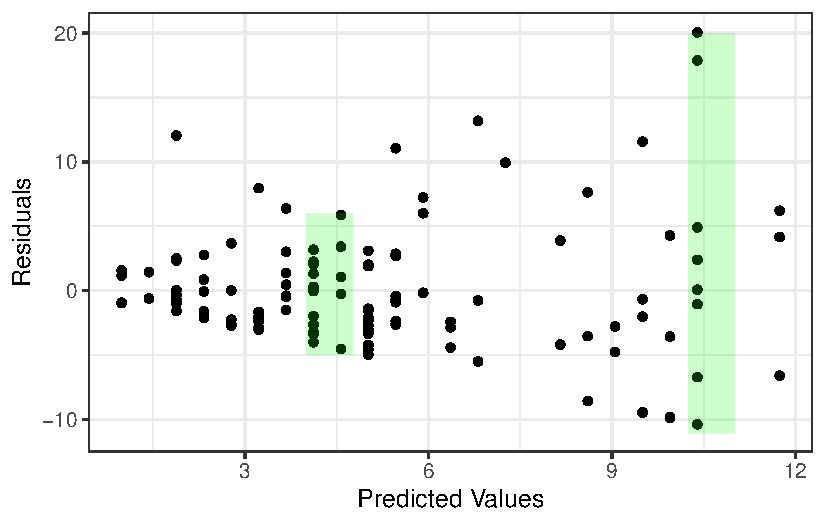
\includegraphics[width=0.8\textwidth,height=\textheight]{./images/fig-regassessment-mean0-1.pdf}

}

\caption{\label{fig-regassessment-mean0}Plot of the residuals vs.~the
predicted values for a model predicting bracketed duration as a function
of the magnitude of an earthquake.}

\end{figure}%

If the errors have a mean of 0 for all values of the predictor, then we
would expect the residuals to have a mean of 0 for all predicted values.
That is, if the data is consistent with the mean-0 condition, then as we
move left to right across the plot, the residuals should tend to balance
out at 0 everywhere along the x-axis. Imagine a ``window'' around the
residuals (shown in the figure as vertical green rectangles), and
imagine moving that window from left to right. If that window has to
shift up or down to contain the cloud of residuals (so that the window
is no longer centered around 0), that indicates a problem. Any trends in
the \emph{location} of this graphic would indicate the data is
\emph{not} consistent with the mean-0 condition.

\begin{tcolorbox}[enhanced jigsaw, breakable, titlerule=0mm, colframe=quarto-callout-note-color-frame, bottomtitle=1mm, opacityback=0, rightrule=.15mm, toptitle=1mm, arc=.35mm, bottomrule=.15mm, left=2mm, title=\textcolor{quarto-callout-note-color}{\faInfo}\hspace{0.5em}{Graphically Assessing the Mean-0 Condition}, leftrule=.75mm, coltitle=black, toprule=.15mm, colbacktitle=quarto-callout-note-color!10!white, colback=white, opacitybacktitle=0.6]

If the data is consistent with the mean-0 condition, there should be no
trends in the \emph{location} of the plot of the residuals against the
predicted values.

\end{tcolorbox}

As we examine Figure~\ref{fig-regassessment-mean0}, the residuals do
tend to balance out at 0 everywhere along the x-axis. That is, we do not
see a trend in the location of the residuals as the predicted values
increase. Therefore, it is reasonable to say the sample is consistent
with the mean-0 condition.

\section{Assessing the Independence
Condition}\label{assessing-the-independence-condition}

\begin{quote}
The error in the bracketed duration for one location is independent of
the error in the bracketed duration for any other location.
\end{quote}

Generally, independence is assessed by considering the method in which
the data was collected and considering the context with a discipline
expert. By carefully considering the manner in which the data was
collected, we can typically determine whether it is reasonable that the
errors in the response are independent of one another. Some key things
to consider when examining the data collection process:

\begin{itemize}
\tightlist
\item
  Are there repeated observations of the same variable made on the same
  subject? This often suggests some type of relationship between the
  observed responses and therefore would not be consistent with errors
  being independent (see Chapter~\ref{sec-blockquestions} and
  Chapter~\ref{sec-blockdata}).
\item
  Is the response measured over time, such as daily temperature over the
  course of a month? Data collected over time often exhibits strong
  period-to-period relationships suggesting the errors are not
  independent. For example, if the temperature today is above average,
  it is more likely to be above average tomorrow as well.
\item
  Is there a learning curve in how the data was collected? Learning
  curves again suggest some dependence from one observation to the next.
  For example, a new nurse may become better at collecting pulse
  readings with more practice over time.
\item
  Measurement devices which are failing over time will introduce a
  dependence from one observation to the next. Imagine a bathroom scale
  that begins to add an additional pound each day. Then, being an above
  average weight one day will most likely lead to an above average
  weight the next, due primarily to the measurement device.
\end{itemize}

These last three points illustrate a particular deviation from our
condition of independence in which two observations collected close
together in time are related. When we know the order in which the data
was collected, we can assess whether the data tends to deviate from the
condition of independence in this manner. This is done graphically
through a \textbf{time-series plot} of the \emph{residuals}. If two
errors were unrelated, then the value of one residual should tell us
nothing about the value of the next residual. Therefore, a plot of the
residuals over time should look like noise (since residuals are supposed
to mimic the noise in the model). If there are any trends, then it
suggests the data is not consistent with independence.

\begin{definition}[Time-Series
Plot]\protect\hypertarget{def-time-series-plot}{}\label{def-time-series-plot}

A time-series plot of a variable is a line plot with the variable on the
y-axis and time on the x-axis.

\end{definition}

\begin{tcolorbox}[enhanced jigsaw, breakable, titlerule=0mm, colframe=quarto-callout-note-color-frame, bottomtitle=1mm, opacityback=0, rightrule=.15mm, toptitle=1mm, arc=.35mm, bottomrule=.15mm, left=2mm, title=\textcolor{quarto-callout-note-color}{\faInfo}\hspace{0.5em}{Graphically Assessing the Independence Condition}, leftrule=.75mm, coltitle=black, toprule=.15mm, colbacktitle=quarto-callout-note-color!10!white, colback=white, opacitybacktitle=0.6]

If the data is consistent with the independence condition, we would not
expect to see a trend in the \emph{location} or \emph{spread} in a
time-series plot of the residuals. Note that this graphic can only be
used if the order in which the data was collected is known, and the
order indicates some natural timing.

\end{tcolorbox}

Figure~\ref{fig-regassessment-independence-violations} shows two
hypothetical datasets. In Panel A, the residuals display a trend in the
location over time. Knowing that a response was below average suggests
the next response will also be below average. In Panel B, the results
display a trend in the spread over time. This suggests that measurements
taken later in the study were less precise. Both panels are examples of
patterns which would suggest the data is not consistent with the
condition of independence.

\begin{figure}

\centering{

\includegraphics[width=0.8\textwidth,height=\textheight]{./images/fig-regassessment-independence-violations-1.pdf}

}

\caption{\label{fig-regassessment-independence-violations}Examples of
trends in a time-series plot of the residuals. Such trends indicate the
data is not consistent with the condition that the errors are
independent of one another.}

\end{figure}%

Instead, if the data were consistent with the condition of independence
on the error terms, we would expect to see a plot similar to
Figure~\ref{fig-regassessment-independence-reasonable}. Notice there are
no trends in the location or spread of the residuals.

\begin{figure}

\centering{

\includegraphics[width=0.8\textwidth,height=\textheight]{./images/fig-regassessment-independence-reasonable-1.pdf}

}

\caption{\label{fig-regassessment-independence-reasonable}Example of a
time-series plot of residuals which shows no trends in location or
spread. This is consistent with what we would expect if the condition of
independence among errors were satisfied.}

\end{figure}%

For the Seismic Activity Case Study, the data was actually collected
over time as earthquakes occurred. More, as technology has changed over
time, it is reasonable to fear that the errors in our observations are
related over time. In order to assess this, consider the time-series
plot of the residuals from our model for the data generating process in
which the bracketed duration is modeled as a linear function of the
magnitude of the earthquake
(Figure~\ref{fig-regassessment-independence}). Based on the figure,
there are no clear trends in either the \emph{location} or \emph{spread}
of the residuals over time (the figure resembles noise with no
patterns). As a result, it is reasonable to assume the data is
consistent with the errors being independent of one another.

\begin{figure}

\centering{

\includegraphics[width=0.8\textwidth,height=\textheight]{./images/fig-regassessment-independence-1.pdf}

}

\caption{\label{fig-regassessment-independence}Time-series plot of the
residuals for a model predicting bracketed duration as a function of the
magnitude of an earthquake.}

\end{figure}%

The condition of independence is another reason we consider
randomization when collecting data. Both random sampling and random
assignment reduces the likelihood of the errors in two observations
being related.

\section{Assessing Homoskedasticity}\label{assessing-homoskedasticity}

\begin{quote}
The variability of the error in the bracketed duration is the same
regardless of the magnitude of the earthquake.
\end{quote}

When assessing the ``mean-0 condition'' above, we saw that the key
phrase was ``for all values of the predictor.'' Similarly,
homoskedasticity suggests the variability in the errors is consistent
\emph{for all values of the predictor}. Therefore, we rely on the same
graphical assessment --- a plot of the residuals against the predicted
values. However, instead of focusing on a trend in the location of the
residuals, we are focused on a trend in the \emph{spread}.

\begin{tcolorbox}[enhanced jigsaw, breakable, titlerule=0mm, colframe=quarto-callout-note-color-frame, bottomtitle=1mm, opacityback=0, rightrule=.15mm, toptitle=1mm, arc=.35mm, bottomrule=.15mm, left=2mm, title=\textcolor{quarto-callout-note-color}{\faInfo}\hspace{0.5em}{Graphically Assessing the Constant Variance Condition}, leftrule=.75mm, coltitle=black, toprule=.15mm, colbacktitle=quarto-callout-note-color!10!white, colback=white, opacitybacktitle=0.6]

If the data is consistent with the constant variance condition, there
should be no trends in the \emph{spread} of the plot of the residuals
against the predicted values.

\end{tcolorbox}

Again, imagine a window (illustrated as vertical green rectangles in
Figure~\ref{fig-regassessment-mean0}) around the residuals. As we move
left to right, if the size of the window has to change in order to keep
the residuals inside (the window stretches or compresses vertically),
then that is an indication that the spread of the residuals is changing.
For our example, there is a clear ``fan shape'' to the residuals as we
move left to right suggesting the precision of the model decreases when
making larger predictions. This goes back to something we observed in
Chapter~\ref{sec-regsummaries} when examining a plot of the response and
predictor (see Figure~\ref{fig-regsummaries-magnitude}). We observed
that for large earthquakes (high magnitudes), the bracketed duration was
much more variable than for smaller earthquakes. So, our model is not as
precise for some values of the predictor. This is evidence that our data
is \emph{not} consistent with the condition that the errors have the
same variability for all values of the predictor.

This partially explains the differences in the confidence intervals
reported in Table~\ref{tbl-regconditions-slr-summary} and
Table~\ref{tbl-regconditions-slr-summary-alt}. Since there is clear
evidence that the data is not consistent with the constant variance
condition, then it is not safe to assume the classical regression model.
That is, the confidence intervals and p-values, as well as the
underlying models for the sampling distribution and null distribution
that generated them, constructed assuming the data is consistent with
all four conditions, are suspect. We should instead rely on an empirical
model for the sampling distribution of the least squares estimates when
constructing confidence intervals or an empirical model for the null
distribution of the standardized statistic if computing a p-value.

\section{Assessing Normality}\label{assessing-normality}

\begin{quote}
The errors in the bracketed duration follow a Normal distribution.
\end{quote}

Assessing whether observations adhere to a particular distribution is a
large area in statistical research. Many methods have been developed for
this purpose. We emphasize a single graphical summary known as a
\textbf{probability plot}. The construction of the plot is beyond the
scope of this text, but the concepts underlying its construction
actually tie in nicely to the big themes we have been discussing. Recall
that if a sample is representative, then it should be a snapshot of the
underlying population. Therefore, if we believe the underlying
population has some particular distribution, we would expect the
properties of this distribution to be apparent in the sample as well.

If we believe the errors follow a Normal distribution, then it is
reasonable that the residuals should maintain some of those properties.
For example, the 10-th percentile of the residuals should roughly equate
to the 10-th percentile expected from a Normal distribution. Mapping the
percentiles that we observe to those that we expect is the essence of a
probability plot.

\begin{definition}[Probability
Plot]\protect\hypertarget{def-probability-plot}{}\label{def-probability-plot}

Also called a ``Quantile-Quantile Plot'', a probability plot is a
graphic for comparing the distribution of an observed sample with a
theoretical probability model for the distribution of the underlying
population. The quantiles observed in the sample are plotted against
those expected under the theoretical model.

\end{definition}

While a probability plot can be constructed for a host of probability
distributions, the most common is the Normal probability plot. The plot
compares the observed residuals with those we would expect if the
residuals were sampled from a Normal distribution. If the residuals
closely aligned with our expectations from a Normal distribution, then
we would expect to see a straight line if these are plotted against one
another. Trends away from a straight line suggest the proposed Normal
distribution is not a reasonable model for the distribution of the
errors.

\begin{tcolorbox}[enhanced jigsaw, breakable, titlerule=0mm, colframe=quarto-callout-note-color-frame, bottomtitle=1mm, opacityback=0, rightrule=.15mm, toptitle=1mm, arc=.35mm, bottomrule=.15mm, left=2mm, title=\textcolor{quarto-callout-note-color}{\faInfo}\hspace{0.5em}{Graphically Assessing the Normality Condition}, leftrule=.75mm, coltitle=black, toprule=.15mm, colbacktitle=quarto-callout-note-color!10!white, colback=white, opacitybacktitle=0.6]

If the data is consistent with the normality condition, the Normal
probability plot of the residuals should exhibit a straight line with
any deviations appearing to be random. Systemic deviations from a
straight line indicate the observed distribution does not align with the
proposed model.

\end{tcolorbox}

Figure~\ref{fig-regassessment-normal} shows the Normal probability plot
of the residuals from our model for the data generating process of the
bracketed duration.

\begin{figure}

\centering{

\includegraphics[width=0.8\textwidth,height=\textheight]{./images/fig-regassessment-normal-1.pdf}

}

\caption{\label{fig-regassessment-normal}Probability plot of the
residuals for a model predicting bracketed duration as a function of the
magnitude of an earthquake.}

\end{figure}%

We note there is some systematic departure from a straight line in the
graphic. In particular, on the left-hand side of the graphic, from -3 to
-1.5 along the x-axis, the points tend to curve upward before changing
direction at -1.5 on the x-axis. While we want to avoid
over-interpreting small deviations from the linear trend, we should pay
attention to clear departures.

We note that of the conditions considered, Normality is probably the
least important as the analytic models for the sampling distributions of
the least squares estimates are generally fairly robust to this
condition. This is especially true in large samples (see
Appendix~\ref{sec-app-theory}). However, we can always relax this
condition by building an empirical model for the sampling distributions
of the least squares estimates. Given the curvature we observed in this
graphic, we would consider an empirical model, especially given we have
already established the data is not consistent with the condition of
homoskedasticity.

For comparison, Figure~\ref{fig-regassessment-normal-comparison}
illustrates a hypothetical dataset for which the residuals suggest the
Normality condition of the errors is unreasonable as well as an example
of when the residuals are consistent with the Normality condition on the
errors.

\begin{figure}

\centering{

\includegraphics[width=0.8\textwidth,height=\textheight]{./images/fig-regassessment-normal-comparison-1.pdf}

}

\caption{\label{fig-regassessment-normal-comparison}Two Normal
probability plots of the residuals for two hypothetical datasets. The
trend away from a straight line in Panel A suggests assuming the errors
follow a Normal distribution would be unreasonable. However, the
reasonably straight line in Panel B suggests the data is consistent with
the errors following a Normal distribution.}

\end{figure}%

\section{General Tips for Assessing
Assumptions}\label{general-tips-for-assessing-assumptions}

Each of the methods presented here are qualitative assessments, which
means they are subjective. That is okay. As the analyst, in consultation
with the discipline expert, it is up to us to determine which conditions
we are willing to assume are reasonable to impose. That is, with which
conditions do we believe the data are consistent? Here are four overall
things to keep in mind.

First, do not spend an extraordinary amount of time examining any one
residual plot. If we stare at a plot too long, we can convince ourselves
there is a pattern in anything. We are looking for glaring evidence that
the data is not consistent with the conditions we have imposed on our
model. This is especially true when we have only a few observations. In
these settings, reading plots can be very difficult. Again, it is about
what we are comfortable assuming.

Second, we have chosen the language carefully throughout this chapter.
We have never once stated that a condition ``was satisfied.'' When we
perform an analysis, we are making an \emph{assumption} that the
conditions are satisfied. We can never prove that they are; we can only
show that the data is consistent with a particular set of conditions. We
can, however, provide evidence that a condition is violated. When that
is the case, we should be wary of trusting the resulting p-values and
confidence intervals which are constructed from imposing that condition.
This is not unlike hypothesis testing; just as we can never prove the
null hypothesis is true, we cannot prove that a condition is satisfied.
The graphics are constructed using residuals, but what we are looking
for comes from how we expect the residuals to behave \emph{if} a
particular condition is true. Just because residuals behave a certain
way, however, does not guarantee a condition is or is not met. Just like
hypothesis testing, we are looking for what we are able to discern given
the data.

\begin{tcolorbox}[enhanced jigsaw, breakable, titlerule=0mm, colframe=quarto-callout-tip-color-frame, bottomtitle=1mm, opacityback=0, rightrule=.15mm, toptitle=1mm, arc=.35mm, bottomrule=.15mm, left=2mm, title=\textcolor{quarto-callout-tip-color}{\faLightbulb}\hspace{0.5em}{Big Idea}, leftrule=.75mm, coltitle=black, toprule=.15mm, colbacktitle=quarto-callout-tip-color!10!white, colback=white, opacitybacktitle=0.6]

We cannot prove a condition is satisfied; we can only hope to show the
data is consistent with the condition and it is therefore reasonable to
\emph{assume} it is satisfied.

\end{tcolorbox}

Third, any conditions required for a particular analysis should be
assessed. If our sample is not consistent with the necessary conditions,
we should choose a different analysis. The inference we obtain from an
analysis is only reliable if the data is consistent with any necessary
conditions.

Finally, transparency is crucial. Perhaps more important than which
conditions we choose to impose is clearly communicating to our audience
our decisions. If our analysis is to be replicated or critiqued fairly
(and any good scientist or engineer should welcome such critique), we
need to be transparent about the decisions we make along the way,
including the assumptions we make on the model for the data generating
process.

\chapter{Extending the Regression Model}\label{sec-regextensions}

The last several chapters have developed an approach for modeling a
quantitative response as a function of a single quantitative predictor
using a model of the form:

\[(\text{Response})_i = \beta_0 + \beta_1 (\text{Predictor})_i + \varepsilon_i.\]

This model is well suited for addressing questions about the marginal
relationship between two variables. However, as we saw in
Chapter~\ref{sec-regquestions}, not all our questions are about the
marginal relationship. The real power of the model in
Equation~\ref{eq-general-model} is our ability to generalize it to
encompass multiple predictors and various types of relationships. In
this chapter, we briefly describe how to extend the regression model to
address some additional questions of interest.

While this chapter can be considered optional for an introductory
treatment to modeling, the concepts discussed here allow us to easily
bridge into the remaining topics covered in later units.

\section{Using a Categorical
Predictor}\label{using-a-categorical-predictor}

We have described the simple linear model (Equation~\ref{eq-slr}) as one
which relates two quantitative variables. However, this framework can be
extended to make use of a categorical predictor. Specifically, we will
consider a binary predictor which categorizes units into one of two
groups. More general categorical predictors will be considered in the
next unit.

Continuing to work with the data from the Seismic Activity Case Study,
Table~\ref{tbl-regextensions-soil} summarizes the bracketed duration at
locations based on the soil conditions.

\begin{table}

\caption{\label{tbl-regextensions-soil}Numerical summaries of the
bracketed duration for locations based on their soil conditions.}

\centering{

\centering
\begin{tabular}[t]{lrrr}
\toprule
Soil Condition & n & Sample Mean & Sample Standard Deviation\\
\midrule
\cellcolor{gray!10}{Intermediate} & \cellcolor{gray!10}{43} & \cellcolor{gray!10}{5.16} & \cellcolor{gray!10}{4.52}\\
Rocky & 24 & 4.14 & 5.72\\
\cellcolor{gray!10}{Soft} & \cellcolor{gray!10}{52} & \cellcolor{gray!10}{5.86} & \cellcolor{gray!10}{6.73}\\
\bottomrule
\end{tabular}

}

\end{table}%

We observe that the bracketed duration appears to differ, on average,
for locations with rocky soils compared to other types of location. We
would like to consider a model for the data generating process of the
form

\[(\text{Bracketed Duration})_i = \beta_0 + \beta_1 (\text{Soil Condition})_i + \varepsilon_i,\]

but the problem is that we do not know how to multiply a number
\(\beta_1\) and a category like ``rocky soil,'' meaning the above model
does not yet even make sense. The key to including a categorical
variable in the model for the data generating process is to construct an
\textbf{indicator variable}.

\begin{definition}[Indicator
Variable]\protect\hypertarget{def-indicator-variable}{}\label{def-indicator-variable}

An indicator variable is a binary (takes the value 0 or 1) variable used
to represent whether an observation belongs to a specific group defined
by a categorical variable.

\end{definition}

Indicator variables essentially create a numeric variable which
represents a yes/no decision regarding a categorical variable. For
example, consider the following variable definition:

\[
(\text{Rocky Soil})_i = \begin{cases} 1 & \text{if } i\text{-th location has rocky soil} \\
0 & \text{if } i\text{-th location has a different soil type}. \end{cases}
\]

Since this variable is numeric, we can use it in our model for the data
generating process. Specifically, consider the following model

\begin{equation}\phantomsection\label{eq-regextensions-ind}{(\text{Bracketed Duration})_i = \beta_0 + \beta_1 (\text{Rocky Soil})_i + \varepsilon_i}\end{equation}

With a variable capturing when the soil is rocky, we might be tempted to
include another indicator variable that takes the value 1 when the soil
is not rocky. But, this is not necessary. Think of an indicator variable
like a ``light switch.'' The indicator variable turns on when an
observation falls into a particular group and turns off otherwise. Just
like a single light switch can place a light into the ``on'' position
and into the ``off'' position, a single indicator variable can capture
two groups in the model for the data generating process. If we have a
location which has ``Intermediate'' soil conditions, then that location
cannot have ``Rocky'' soil; therefore, the indicator variable in our
model turns off. Setting the indicator to 0 (turning it ``off'') then
leaves only the intercept in the model. The group which has a 0 for the
indicator is encoded in the intercept; this is known as the
\textbf{reference group}.

\begin{definition}[Reference
Group]\protect\hypertarget{def-reference-group}{}\label{def-reference-group}

The group defined by setting all indicator variables in a model for the
data generating process equal to 0.

\end{definition}

Remember, provided that we have imposed the mean-0 condition, we know
that the deterministic portion of the model specifies the mean response
for a given value of the predictor. In the case of an indicator
variable, the predictor variable can only take on two values (0 or 1).
Therefore, it only predicts two mean responses:

\begin{itemize}
\tightlist
\item
  When the indicator variable is 0, the model predicts a mean response
  of \(\beta_0\); and,
\item
  When the indicator variable is 1, the model predicts a mean response
  of \(\beta_0 + \beta_1\).
\end{itemize}

So, the ``slope'' \(\beta_1\) is really capturing the shift in the
deterministic portion of the model from one group to the other. This
coincides with the interpretation of the slope discussed in
Chapter~\ref{sec-regconditions} --- \(\beta_1\) represents the change in
the mean response when moving from one group to another. That is, the
slope represents the difference in the average response between the two
groups.

\begin{tcolorbox}[enhanced jigsaw, breakable, titlerule=0mm, colframe=quarto-callout-note-color-frame, bottomtitle=1mm, opacityback=0, rightrule=.15mm, toptitle=1mm, arc=.35mm, bottomrule=.15mm, left=2mm, title=\textcolor{quarto-callout-note-color}{\faInfo}\hspace{0.5em}{Interpretation of the Parameters}, leftrule=.75mm, coltitle=black, toprule=.15mm, colbacktitle=quarto-callout-note-color!10!white, colback=white, opacitybacktitle=0.6]

Suppose we have a simple linear regression model (Equation~\ref{eq-slr})
with a quantitative response and a single indicator variable as the sole
predictor. Then, the intercept represents the average response for the
reference group, and the slope represents the difference in the average
response between the two groups.

\end{tcolorbox}

This shift in the mean response is illustrated in
Figure~\ref{fig-regextensions-ind-plot}. The ``line'' is really
connecting the sample mean response of each group.

\begin{figure}

\centering{

\includegraphics[width=0.8\textwidth,height=\textheight]{./images/fig-regextensions-ind-plot-1.pdf}

}

\caption{\label{fig-regextensions-ind-plot}Comparison of the bracketed
duration between locations with rocky soil and those with other soil
types.}

\end{figure}%

\section{Including Multiple
Precitors}\label{including-multiple-precitors}

The real power of the model in Equation~\ref{eq-general-model} is our
ability to generalize it to encompass multiple predictors and various
types of relationships. That is, suppose that instead of being
interested in the marginal relationship between the bracketed duration
and the magnitude of the corresponding earthquake we are interested in
\emph{isolating} the effect of the magnitude on the bracketed duration:

\begin{quote}
On average, does the bracketed duration change as the magnitude of the
corresponding earthquake changes if the location remains the same
distance from the center of the earthquake?
\end{quote}

This question is asking if there is an effect of the magnitude of the
earthquake above and beyond the impact due to a locations distance from
the epicenter. This question requires a model which has multiple
predictors. What bracketed duration would we expect given the magnitude
and epicentral distance? We extend the simple linear model to include an
additional predictor:

\begin{equation}\phantomsection\label{eq-regextensions-mlr}{(\text{Bracketed Duration})_i = \beta_0 + \beta_1(\text{Magnitude})_i + \beta_2(\text{Epicentral Distance})_i + \varepsilon_i.}\end{equation}

This more complex model is more difficult to visualize, but conceptually
it is similar to the simple linear model in Equation~\ref{eq-slr}. Given
a value for the magnitude \emph{and} epicentral distance, we can predict
the bracketed duration; the model for the data generating process allows
both variables to contribute to the bracketed duration. Our model for
the data generating process also allows for random noise to contribute
to the bracketed duration; that is, there will still be unexplained
variability. One way of envisioning what this model does is to think
about taking the linear relationship we previously had and observing
that we are now saying that the deterministic portion of the model for
the data generating process differs for each group of observations which
have a different epicentral distance. For example, consider all
locations which were located 10 km away from the center of an
earthquake; for this group of earthquakes,
Equation~\ref{eq-regextensions-mlr} suggests the bracketed duration is
generated by

\[
\begin{aligned}
(\text{Bracketed Duration})_i 
  &= \beta_0 + \beta_1(\text{Magnitude})_i + \beta_2(10) + \varepsilon_i \\
  &= \left(\beta_0 + 10\beta_2\right) + \beta_1(\text{Magnitude})_i + \varepsilon_i.
\end{aligned}
\]

Similarly, if we only consider locations which were located 32 km away
from the center of an earthquake, then
Equation~\ref{eq-regextensions-mlr} suggests the bracketed duration is
generate by

\[
\begin{aligned}
(\text{Bracketed Duration})_i 
  &= \beta_0 + \beta_1(\text{Magnitude})_i + \beta_2(32) + \varepsilon_i \\
  &= \left(\beta_0 + 32\beta_2\right) + \beta_1(\text{Magnitude})_i + \varepsilon_i.
\end{aligned}
\]

Figure~\ref{fig-regextensions-mlr-plot} represents this graphically for
a range of potential epicentral distances. Essentially, the relationship
between the bracketed duration and the magnitude shifts depending on the
epicentral distance. The overall trend is similar (the lines are
parallel), but where the line is located is really dependent upon the
distance of the location from the earthquake. Note that while
Figure~\ref{fig-regextensions-mlr-plot} chooses particular values for
the epicentral distance, we could have easily made an analogous graphic
which chooses values for the magnitude and envisions the relationship
between the bracketed duration and the epicentral distance for each of
these choices.

\begin{figure}

\centering{

\includegraphics[width=0.8\textwidth,height=\textheight]{./images/fig-regextensions-mlr-plot-1.pdf}

}

\caption{\label{fig-regextensions-mlr-plot}Relationship between the
bracketed duration and the magnitude of an earthquake after also
considering the epicentral distance from an earthquake. Lines estimating
this relationship for various values of the epicentral distance are
overlayed.}

\end{figure}%

This model has what may appear as an obvious requirement; you cannot use
this model to predict the bracketed duration without specifying
\emph{both} the magnitude of the earthquake and the epicentral distance
of the location. However, it also isolates the effect of the magnitude
above and beyond the epicentral distance.

\subsection{General Model Formulation}\label{general-model-formulation}

Nothing limits us from the inclusion of several predictors. Each
predictor is simply added to the model.

\begin{tcolorbox}[enhanced jigsaw, breakable, titlerule=0mm, colframe=quarto-callout-important-color-frame, bottomtitle=1mm, opacityback=0, rightrule=.15mm, toptitle=1mm, arc=.35mm, bottomrule=.15mm, left=2mm, title=\textcolor{quarto-callout-important-color}{\faExclamation}\hspace{0.5em}{General Linear Regression Model}, leftrule=.75mm, coltitle=black, toprule=.15mm, colbacktitle=quarto-callout-important-color!10!white, colback=white, opacitybacktitle=0.6]

For a quantitative response and one or more predictors, the general form
of the linear regression model is

\begin{equation}\phantomsection\label{eq-mlr}{
\begin{aligned}
  (\text{Response})_i 
    &= \beta_0 + \beta_1 (\text{Predictor 1})_i + \beta_2(\text{Predictor 2})_i + \dotsb + \beta_p (\text{Predictor } p)_i + \varepsilon_i \\
    &= \beta_0 + \sum_{j=1}^{p} \beta_j (\text{Predictor j})_i + \varepsilon_i
\end{aligned}
}\end{equation}

where \(\beta_j\) for \(j = 0, 1, 2, \dotsc, p\) are the \(p + 1\)
parameters governing the model for the data generating process.

\end{tcolorbox}

\begin{tcolorbox}[enhanced jigsaw, breakable, titlerule=0mm, colframe=quarto-callout-note-color-frame, bottomtitle=1mm, opacityback=0, rightrule=.15mm, toptitle=1mm, arc=.35mm, bottomrule=.15mm, left=2mm, title=\textcolor{quarto-callout-note-color}{\faInfo}\hspace{0.5em}{Note}, leftrule=.75mm, coltitle=black, toprule=.15mm, colbacktitle=quarto-callout-note-color!10!white, colback=white, opacitybacktitle=0.6]

The predictors in Equation~\ref{eq-mlr} can be quantitative variables or
indicator variables (Definition~\ref{def-indicator-variable}).

\end{tcolorbox}

The problem, of course, is that the parameters (the \(\beta\)'s in the
model) are unknown. However, we can use the method of least squares to
estimate each of the parameters simultaneously.

\begin{definition}[Least Squares Estimates for General Linear
Model]\protect\hypertarget{def-mlr-least-squares-estimates}{}\label{def-mlr-least-squares-estimates}

The least squares estimates for a general linear model
(Equation~\ref{eq-mlr}) are the values of
\(\beta_0, \beta_1, \beta_2, \dotsc, \beta_p\) which minimize the
quantity

\[\sum_{i=1}^n \left[(\text{Response})_i - \beta_0 - \sum_{j=1}^{p} \beta_j(\text{Predictor } j)_{i}\right]^2.\]

\end{definition}

This minimization procedure is implemented in any statistical software
package.

\subsection{Interpretation of
Parameters}\label{interpretation-of-parameters}

The same conditions described in Chapter~\ref{sec-regconditions} can be
placed on the stochastic portion of the model for the data generating
process. Just as with the simple linear model, assuming the model is
correctly specified (imposing the mean-0 condition) provides us with an
interpretation of each of the parameters.

Consider the model for the data generating process defined in
Equation~\ref{eq-regextensions-mlr}. If we assume that the error in the
bracketed duration has an average of 0 regardless of the magnitude of
the corresponding earthquake and the distance of the location to the
center of the earthquake, then notice that we are saying the expression

\[\beta_0 + \beta_1(\text{Magnitude}) + \beta_2(\text{Epicentral Distance})\]

defines the average bracketed duration (given the magnitude of the
earthquake and epicentral distance of the location).

\begin{tcolorbox}[enhanced jigsaw, breakable, titlerule=0mm, colframe=quarto-callout-tip-color-frame, bottomtitle=1mm, opacityback=0, rightrule=.15mm, toptitle=1mm, arc=.35mm, bottomrule=.15mm, left=2mm, title=\textcolor{quarto-callout-tip-color}{\faLightbulb}\hspace{0.5em}{Big Idea}, leftrule=.75mm, coltitle=black, toprule=.15mm, colbacktitle=quarto-callout-tip-color!10!white, colback=white, opacitybacktitle=0.6]

If we impose the mean-0 condition, the deterministic portion of the
general linear regression model specifies the mean response given the
value of the predictors.

\end{tcolorbox}

Therefore, we can interpret the value of \(\beta_2\) as the change in
the average bracketed duration given a 1-kilometer increase in the
distance a location is from the center of the earthquake \emph{for all
locations which experience an earthquake of the same magnitude}. This
last part is important. In order to interpret one coefficient, we must
hold the value of all other predictors fixed.

\begin{tcolorbox}[enhanced jigsaw, breakable, titlerule=0mm, colframe=quarto-callout-note-color-frame, bottomtitle=1mm, opacityback=0, rightrule=.15mm, toptitle=1mm, arc=.35mm, bottomrule=.15mm, left=2mm, title=\textcolor{quarto-callout-note-color}{\faInfo}\hspace{0.5em}{Interpretation of Parameters}, leftrule=.75mm, coltitle=black, toprule=.15mm, colbacktitle=quarto-callout-note-color!10!white, colback=white, opacitybacktitle=0.6]

For the general linear model (Equation~\ref{eq-mlr}), the intercept
\(\beta_0\) is the average response when \emph{all} predictors are set
equal to 0. The \(j\)-th coefficient \(\beta_j\) represents the average
change in the response associated with a 1-unit increase in the \(j\)-th
predictor holding the value of all other predictors constant.

\end{tcolorbox}

This phrase ``holding the value of all other predictors constant'' has
extreme power. It is because of this phrase that we are able to take our
first steps toward addressing confounding. For example, consider the
model for the data generating process in
Equation~\ref{eq-regextensions-mlr}. Using the method of least squares,
we estimate that for every kilometer further the epicenter of the
earthquake is, we can expect the bracketed duration to decrease by 0.08
seconds, on average. Someone might argue as follows: ``This is not a
controlled experiment; therefore, while there is an association here, it
is possible that what is really happening is that earthquakes which were
further away tended to also be smaller in magnitude. Therefore, it is
not the distance that is driving this observed association but the
magnitude of the earthquake.'' Here, this individual is saying that the
earthquake's magnitude is a confounder --- related to both the bracketed
duration (response) and the variable of interest (distance from the
epicenter). If we had fit a marginal model, this would be a valid
concern. However, remember our interpretation of \(\beta_2\) (and our
estimate of it) --- our fit suggests that for every kilometer further
the epicenter of the earthquake is, we can expect the bracketed duration
to decrease by 0.08 seconds, on average, \emph{holding the magnitude of
the earthquake constant}. Therefore, since this estimate is comparing
two earthquakes of the same magnitude, magnitude cannot be confounding
the relationship observed. We have isolated the effect of the epicentral
distance from any effect due to the magnitude.

Our solution to confounding is to incorporate the relationship between
the confounder and the response into our model for the data generating
process. Then, any remaining variables cannot be affected by the
confounder. Of course this has one major limitation --- we cannot
account for any variables which are not recorded.

There are entire texts devoted to the topic of addressing confounding.
Here, we simply emphasize that regression models allow us to control for
the confounders we have observed. The relationships are ``adjusted for''
these confounders due to the interpretation that a coefficient is the
effect ``holding all other predictors constant.'' Regression models
allow us to compare similar groups, which are balanced on these
confounders after the fact (instead of having addressed confounding
through the design of the study).

\subsection{Inference for the General
Formulation}\label{inference-for-the-general-formulation}

Above, we estimated the change in the average bracketed duration
associated with a 1 kilometer increase in the distance from an
earthquake while holding the magnitude of the earthquake fixed. However,
as we have noted throughout the text, inference requires that we
quantify the variability in those estimates.

The same processes that allowed us to model the sampling of the least
squares estimates for the simple linear regression model, described in
Chapter~\ref{sec-regconditions}, are applicable for the general linear
regression model as well. In particular, under the classical regression
model (imposing all four conditions discussed in
Chapter~\ref{sec-regconditions} on the error term), we can construct an
analytical model of the sampling distribution of the least squares
estimates (extensions of the results discussed in
Appendix~\ref{sec-app-theory}). And, provided we are willing to impose
the mean-0 condition and the independence condition, we can construct an
empirical model of the sampling distribution using a bootstrapping
algorithm. Once we have a model for the sampling distribution of our
estimates, we can construct confidence intervals.

Table~\ref{tbl-regextensions-ci} provide a summary of using the data
from the Seismic Activity Case Study to fit the model for the data
generating process proposed in Equation~\ref{eq-regextensions-mlr}; the
confidence intervals were computed assuming the data was consistent with
all four conditions of the classical regression model.

\begin{table}

\caption{\label{tbl-regextensions-ci}Summary the linear model fit
relating the bracketed duration at locations in Greece following an
earthquake with the magnitude of the event and the distance of the
location from the center of the earthquake.}

\centering{

\centering
\begin{tabular}[t]{lrrrr}
\toprule
Term & Estimate & Standard Error & Lower 95\% CI & Upper 95\% CI\\
\midrule
\cellcolor{gray!10}{(Intercept)} & \cellcolor{gray!10}{-30.715} & \cellcolor{gray!10}{4.887} & \cellcolor{gray!10}{-40.395} & \cellcolor{gray!10}{-21.036}\\
Magnitude & 6.991 & 0.964 & 5.082 & 8.900\\
\cellcolor{gray!10}{Epicentral Distance} & \cellcolor{gray!10}{-0.077} & \cellcolor{gray!10}{0.021} & \cellcolor{gray!10}{-0.118} & \cellcolor{gray!10}{-0.036}\\
\bottomrule
\end{tabular}

}

\end{table}%

From the output, we estimate that for every kilometer further the
epicenter of the earthquake is, it is reasonable to expect the bracketed
duration to decrease between 0.036 and 0.118 seconds, on average,
holding the magnitude of the earthquake fixed.

If we are interested in comparing two models, we formulate a
standardized statistic and model its null distribution. Suppose for the
model we have been considering, we are interested in testing

\[H_0: \beta_1 = \beta_2 = 0 \qquad \text{vs.} \qquad \text{At least one } \beta_j \text{ differs from 0},\]

which corresponds to the following research question:

\begin{quote}
Does the study provide evidence that the average bracketed duration
depends on either the magnitude of the earthquake or the epicentral
distance?
\end{quote}

Note the complexity of this question and the corresponding hypotheses.
We are wanting to drop out two terms from the model for the data
generating process. Just as in Chapter~\ref{sec-regquality}, the key to
testing this hypothesis is to partition out the sources of variability.
We can define the error sums of squares for the general linear
regression model:

\[SSE = \sum_{i=1}^{n}\left[(\text{Response})_i - \sum_{j=1}^{p} \beta_j (\text{Predictor } j)_i\right]^2.\]

The above hypotheses suggest two alternate models for the data
generating process. Under the alternative hypothesis, we have the full
unconstrained model presented in Equation~\ref{eq-regextensions-mlr}
(call that Model 1). Under the null hypothesis, we have a reduced
constrained model for the data generating process (call it Model 0):

\[(\text{Bracketed Duration})_i = \beta_0 + \varepsilon_i.\]

If the null hypothesis is true, we would expect the amount of
unexplained variability in Model 0 to be the same as the amount of
unexplained variability in Model 1 \(\left(SSE_0 \approx SSE_1\right)\).
That is, if the model under the null hypothesis is sufficient for
explaining the variability in the bracketed duration, then it should
perform as well as the full unconstrained model. If, however, Model 1
explains more of the variability in the bracketed duration (therefore
leaving less variability unexplained) than Model 0, then this would
indicate the null hypothesis is false. This suggests that a metric for
quantifying the signal in the data is given by

\[SSE_0 - SSE_1,\]

where we use the subscript to denote the model from which the sum of
squares was computed. As in Chapter~\ref{sec-regquality}, working with
variance terms is easier than working with sums of squares analytically.
And, we need to consider the size of the signal relative to the amount
of background noise. This leads to a form of our standardized statistic
which generalizes our result from Definition~\ref{def-standard-f}.

\begin{definition}[Standardized Statistic for General Linear
Model]\protect\hypertarget{def-general-f}{}\label{def-general-f}

Consider testing a set of hypotheses for a model of the data generating
process of the form (Equation~\ref{eq-mlr}):

\[(\text{Response})_i = \beta_0 + \sum_{j=1}^{p} \beta_j(\text{Predictor } j)_i + \varepsilon_i.\]

Denote this model as Model 1, and denote the model that results from
applying the parameter constraints defined under the null hypothesis as
Model 0. A standardized statistic, sometimes called the ``nested F
statistic,'' for testing the hypotheses is given by

\[T^* = \frac{\left(SSE_0 - SSE_1\right) / (p + 1 - r)}{SSE_1 / (n - p - 1)},\]

where \(p + 1\) is the number of parameters in the full unconstrained
model (including the intercept) and \(r\) is the number of parameters in
the reduced model. Defining

\[MSA = \frac{SSE_0 - SSE_1}{p + 1 - r}\]

to be the ``mean square for additional terms,'' which captures the shift
in the error sum of squares from the reduced model to the full
unconstrained model, we can write the standardized statistic as

\[T^* = \frac{MSA}{MSE}\]

where the mean square error in the denominator comes from the full
unconstrained model. Just as before, the MSE represents the residual
variance --- the variance in the response for a particular set of the
predictors.

\end{definition}

The standardized statistics in Chapter~\ref{sec-teststat} and in
Chapter~\ref{sec-regquality} are special cases of the one presented
here. The numerator captures the signal by examining the difference
between what we expect the error sum of squares to be under the null
hypothesis and what we actually observe; the denominator captures the
background noise (relative to the estimated mean response from the full
model). Larger values of this standardized statistic indicate more
evidence in the sample against the null hypothesis.

Table~\ref{tbl-regextensions-p} provides a summary of partitioning the
variability to test the hypotheses described above using the data from
the Seismic Activity Case Study; the p-value was computed assuming the
data was consistent with all four conditions of the classical regression
model.

\begin{table}

\caption{\label{tbl-regextensions-p}Analysis of the sources of
variability in the bracketed duration as a function of the magnitude of
the earthquake and the epicentral distance.}

\centering{

\centering\centering
\resizebox{\ifdim\width>\linewidth\linewidth\else\width\fi}{!}{
\begin{tabular}[t]{lrrrrl}
\toprule
Term & DF & Sum of Squares & Mean Square & Standardized Statistic & P-Value\\
\midrule
\cellcolor{gray!10}{\cellcolor{gray!10}{Additional Terms}} & \cellcolor{gray!10}{\cellcolor{gray!10}{2}} & \cellcolor{gray!10}{\cellcolor{gray!10}{1297.653}} & \cellcolor{gray!10}{\cellcolor{gray!10}{648.827}} & \cellcolor{gray!10}{\cellcolor{gray!10}{28.17}} & \cellcolor{gray!10}{\cellcolor{gray!10}{< 0.001}}\\
Error & 116 & 2671.787 & 23.033 &  & \\
\bottomrule
\end{tabular}}

}

\end{table}%

Based on the results, the sample provides strong evidence
(\(p < 0.001\)) that the average bracketed duration is associated with
either (or both) the magnitude of the earthquake and the distance the
location is from the center of the earthquake. Note that the p-value
does not tell us the form of the relationship, or whether it is only one
of the predictors that is important or both. Examining the confidence
intervals provides that information. The confidence intervals also allow
a discipline expert to determine if the signal we are discerning is
meaningful in practice.

\section{Modifying an Effect}\label{modifying-an-effect}

There is one type of question we have not yet addressed --- assessing
the interplay between two variables on the response.

Consider the following question:

\begin{quote}
Is the relationship between the average bracketed distance and the
magnitude different depending on whether the soil is rocky where the
measurement is taken?
\end{quote}

This question explains the bracketed duration in terms of both the
magnitude as well as whether the soil is rocky. A first pass at such a
model might be

\[
(\text{Bracketed Duration})_i = \beta_0 + \beta_1(\text{Magnitude})_i + \beta_2(\text{Rocky Soil})_i + \varepsilon_i
\]

where we use an indicator variable to capture whether the soil is rocky
just as before. Just as we did before, we can graphically represent this
model (see Figure~\ref{fig-regextensions-ind-plot2}), and we find that
it is captured by two parallel lines.

\begin{figure}

\centering{

\includegraphics[width=0.8\textwidth,height=\textheight]{./images/fig-regextensions-ind-plot2-1.pdf}

}

\caption{\label{fig-regextensions-ind-plot2}Relationship between the
bracketed duration and magnitude for locations with rocky soil and those
with other soil types.}

\end{figure}%

The lines are parallel because the coefficient associated with Magnitude
\(\left(\beta_1\right)\) is the same regardless of the type of soil.
That is, regardless of whether the soil is rocky, the change in the
bracketed duration, on average, for each 1-unit increase in the
magnitude of an earthquake is the same. Our question of interest is
essentially, is there evidence that this is not the case? So, the above
model actually represents the model for the data generating process
under the null hypothesis of our current question. Under the null
hypothesis, the effect of the magnitude on the bracketed duration (which
captures the relationship between these two variables) is the same
regardless of soil condition. What we posited above is Model 0 which has
an embedded constraint. The question is, how do we form the model for
the data generating process which allows the slope to look differently
depending on soil type? This new model would serve as our full
unconstrained model, Model 1.

Consider adding an additional term to our model above, yielding the
following model:

\[
\begin{aligned}
  (\text{Bracketed Duration})_i 
    &= \beta_0 + \beta_1 (\text{Magnitude})_i + \beta_2 (\text{Rocky Soil})_i \\
    &\qquad + \beta_3 (\text{Magnitude})_i (\text{Rocky Soil})_i + \varepsilon_i
\end{aligned}
\]

This additional term is formed by taking the product of the indicator
variable with the variable magnitude; such a product is known as an
\textbf{interaction term}.

\begin{definition}[Interaction
Term]\protect\hypertarget{def-interaction-term}{}\label{def-interaction-term}

A variable resulting from taking the product of two predictors in a
regression model. The product allows the effect of one predictor to
depend on another predictor, essentially modifying the effect.

\end{definition}

In order to really see the impact of the interaction term, observe that
if we impose the mean-0 condition, our model for the data generating
process says the average bracketed duration for locations with rocky
soil is given by

\[\left(\beta_0 + \beta_2\right) + \left(\beta_1 + \beta_3\right) (\text{Magnitude})\]

which comes from plugging in 1 for the indicator variable (representing
rocky soils) and then combining terms. The model for the data generating
process says the average bracketed duration for locations without rocky
soil is given by

\[\beta_0 + \beta_1 (\text{Magnitude})\]

since we would plug in 0 for the indicator variable (representing soils
that are not rocky). Therefore, our revised model for the data
generating process that includes the interaction term allows both the
intercept and the effect of the magnitude on the bracketed duration to
differ for rocky soils and non-rocky soils. That is, the effect of
magnitude is allowed to differ across the soil types.

\begin{tcolorbox}[enhanced jigsaw, breakable, titlerule=0mm, colframe=quarto-callout-tip-color-frame, bottomtitle=1mm, opacityback=0, rightrule=.15mm, toptitle=1mm, arc=.35mm, bottomrule=.15mm, left=2mm, title=\textcolor{quarto-callout-tip-color}{\faLightbulb}\hspace{0.5em}{Big Idea}, leftrule=.75mm, coltitle=black, toprule=.15mm, colbacktitle=quarto-callout-tip-color!10!white, colback=white, opacitybacktitle=0.6]

It is common to believe that the interaction term measures the effect
between the two variables in the product. However, this is incorrect.
The interaction term allows the effect of one predictor to differ across
the levels of another predictor.

\end{tcolorbox}

Visually, this revised model allows two completely different
associations --- depending on the soil type. This is shown in
Figure~\ref{fig-regextensions-int-plot}. Notice that the lines are no
longer parallel. The question of course is which of the two models is
more appropriate. Is there actually evidence that the more complex
model, which allows the relationship to differ for locations with
different soil types, is required? Or, is the more simplistic model,
which says the relationship is the same across all locations of
different soil types, sufficient?

\begin{figure}

\centering{

\includegraphics[width=0.8\textwidth,height=\textheight]{./images/fig-regextensions-int-plot-1.pdf}

}

\caption{\label{fig-regextensions-int-plot}Relationship between
bracketed duration and the magnitude of an earthquake after also
considering the soil conditions of the measurement location. The
relationship between the bracketed duration and the magnitude is allowed
to differ within each type of soil condition.}

\end{figure}%

We can capture our question of interest in the following hypotheses:

\begin{quote}
\(H_0: \beta_3 = 0\)\\
\(H_1: \beta_3 \neq 0\)
\end{quote}

Notice that if the null hypothesis were true, then the slope would be
the same regardless of whether the soil was rocky because we resort to
Model 0 described above which only allows the intercept to vary across
soil types. However, if \(\beta_3\) is nonzero in Model 1, then the
slope will differ for the rocky soil. So, under the null hypothesis, the
lines are parallel; under the alternative hypothesis, the lines are not
parallel.

Conceptually, comparing these two models is just like any other
hypothesis test. By partitioning the variability as described in the
previous section, we are able to compute a signal-to-noise ratio. We can
essentially determine how much variability in the response is explained
is by the inclusion of the interaction term. That is, we quantify how
the unexplained variability decreases when we include the interaction
term in the model for the data generating process.

Specifically, Table~\ref{tbl-regextensions-fit} gives the estimates
associated with each parameter, and Table~\ref{tbl-regextensions-anova}
presents the corresponding partitioning of the sources of variability
leading to the computation of the p-value. The confidence intervals and
p-value are computed assuming the data is consistent with the conditions
of the classical regression model.

\begin{table}

\caption{\label{tbl-regextensions-fit}Summary of the model fit
explaining the bracketed duration as a function of both magnitude and
soil condition at the measurement location. The effect of the magnitude
was allowed to differ across soil conditions.}

\centering{

\centering\centering
\resizebox{\ifdim\width>\linewidth\linewidth\else\width\fi}{!}{
\begin{tabular}[t]{lrrrr}
\toprule
Term & Estimate & Standard Error & 95\% Lower CI & 95\% Upper CI\\
\midrule
\cellcolor{gray!10}{\cellcolor{gray!10}{(Intercept)}} & \cellcolor{gray!10}{\cellcolor{gray!10}{-23.966}} & \cellcolor{gray!10}{\cellcolor{gray!10}{4.531}} & \cellcolor{gray!10}{\cellcolor{gray!10}{-32.941}} & \cellcolor{gray!10}{\cellcolor{gray!10}{-14.991}}\\
Magnitude & 5.466 & 0.834 & 3.814 & 7.118\\
\cellcolor{gray!10}{\cellcolor{gray!10}{Soil Conditions (Rocky)}} & \cellcolor{gray!10}{\cellcolor{gray!10}{11.925}} & \cellcolor{gray!10}{\cellcolor{gray!10}{9.181}} & \cellcolor{gray!10}{\cellcolor{gray!10}{-6.261}} & \cellcolor{gray!10}{\cellcolor{gray!10}{30.112}}\\
Interaction: Magnitude \& Rocky Soil & -2.614 & 1.626 & -5.835 & 0.607\\
\bottomrule
\end{tabular}}

}

\end{table}%

\begin{table}

\caption{\label{tbl-regextensions-anova}Table partitioning the sources
of variability corresponding to testing whether the effect of the
magnitude of an earthquake on the resulting bracketed duration differs
across soil conditions.}

\centering{

\centering
\begin{tabular}[t]{lrrrrr}
\toprule
Source & DF & SS & MS & Standardized Statistic & P-Value\\
\midrule
\cellcolor{gray!10}{Additional Terms} & \cellcolor{gray!10}{1} & \cellcolor{gray!10}{62.663} & \cellcolor{gray!10}{62.663} & \cellcolor{gray!10}{2.584} & \cellcolor{gray!10}{0.111}\\
Error & 115 & 2788.908 & 24.251 &  & \\
\bottomrule
\end{tabular}

}

\end{table}%

From our analysis, our data is consistent with (\(p = 0.111\)) the
effect of the magnitude being the same across the various soil
conditions. The sample provides no evidence that the association between
the average bracketed duration and the magnitude of an earthquake
depends on the soil conditions.

\chapter{Putting it All Together}\label{sec-regrecap}

For the Seismic Activity Case Study, consider the following question:

\begin{quote}
Overall, does the average bracketed duration at a location depend on the
distance a location is from the center of an earthquake?
\end{quote}

While we have touched on this question in previous chapters, we
investigate this question more fully in this chapter.

\section{Graphical Summary}\label{graphical-summary}

Before developing a statistical model to address our question, we
summarize the data graphically. The question suggests the bracketed
duration is the response variable and the epicentral distance is the
predictor. Figure~\ref{fig-regrecap-plot} illustrates the relationship
between the bracketed duration and the epicentral distance. We note that
the axis for the epicentral distance takes logarithmic steps to better
illustrate the relationship. That is, moving from 1 to 10 kilometers has
roughly the same effect as moving from 10 to 100 kilometers from the
earthquake.

\begin{figure}

\centering{

\includegraphics[width=0.8\textwidth,height=\textheight]{./images/fig-regrecap-plot-1.pdf}

}

\caption{\label{fig-regrecap-plot}Relationship between the bracketed
duration and the distance from the epicenter of an earthquake for
locations measuring seismic activity in Greece.}

\end{figure}%

\section{Development of Statistical
Model}\label{development-of-statistical-model}

In order to address our primary question of interest, we must develop a
statistical model which explains the data generating process and embeds
our question of interest in terms of the parameters of the model. Based
on the question of interest, and our observations in the graphical
exploration above, our model explaining the generation of the bracketed
duration should depend on the epicentral distance. Further, this
relationship should be on a logarithmic scale to account for the
``stretched'' scale in Figure~\ref{fig-regrecap-plot}.

At first, it may seem that the logarithmic scale prevents our use of the
``linear'' model we discussed in this unit, but the model is flexible
enough to accommodate this development. We propose the following model
for the data generating process:

\begin{equation}\phantomsection\label{eq-regrecap-model}{(\text{Bracketed Duration})_i = \beta_0 + \beta_1 \log_{10}(\text{Epicentral Distance})_i + \varepsilon_i.}\end{equation}

Notice that instead of just the epicentral distance, our predictor is
the base-10 logarithm of the epicentral distance. This transformed
variable enters the model just as any other predictor. In addition to
modeling the deterministic portion of the data generating process, we
must also place conditions on the stochastic portion in order to make
inference. We consider the conditions of the classical regression model:

\begin{itemize}
\tightlist
\item
  The error in the bracketed duration is 0, on average for all
  epicentral distances; that is, the model for the deterministic portion
  is correctly specified.
\item
  The error in the bracketed duration for one location is independent of
  the error in the bracketed duration for any other location.
\item
  The variability of the error in the bracketed duration is the same for
  all locations regardless of the epicentral distance.
\item
  The error in the bracketed duration follows a Normal distribution.
\end{itemize}

Before imposing these conditions, however, we should assess them.

\section{Assessment of Conditions}\label{assessment-of-conditions}

Before making inference regarding our question of interest, we should
determine if our data is consistent with the conditions on the error
term we have specified. Figure~\ref{fig-regrecap-normality} is a
probability plot of the residuals used to assess whether the data is
consistent with the Normality condition.

\begin{figure}

\centering{

\includegraphics[width=0.8\textwidth,height=\textheight]{./images/fig-regrecap-normality-1.pdf}

}

\caption{\label{fig-regrecap-normality}Normal probability plot of the
residuals corresponding to a model for the bracketed duration of seismic
events in Greece as a function of the epicentral distance.}

\end{figure}%

The plot reveals some departure from the linear relationship we would
expect if the errors followed a Normal distribution. It seems
unreasonable to impose the Normality condition.

Figure~\ref{fig-regrecap-indep} is a plot of the residuals for the
observations in the order in which they were collected. Since the data
was collected over time, this plot could reveal potential patterns among
the residuals which suggest a departure from independence among the
errors. As there are no trends in either the location or spread of the
residuals, the data is consistent with the independence conditions.

\begin{figure}

\centering{

\includegraphics[width=0.8\textwidth,height=\textheight]{./images/fig-regrecap-indep-1.pdf}

}

\caption{\label{fig-regrecap-indep}Time-series plot of the residuals
corresponding to a model for the bracketed duration of seismic events in
Greece as a function of the epicentral distance.}

\end{figure}%

Figure~\ref{fig-regrecap-mean0} is a plot of the residuals against the
predicted values from the deterministic portion of the model. There are
no obvious trends in the location of the residuals; that is, the
residuals balance out around 0 for all predicted values. Therefore, we
are willing to the data is consistent with the condition that the mean
of the errors is 0 for each combination of the predictors. We note that
while the points balance out around 0 (as indicated by a smoother that
remains near 0), they tend to have a larger range on the positive side
compared to the negative side; this relates back the observation we made
earlier that the residuals do not behave like a sample from a Normal
distribution.

We also note that the spread of the residuals is larger on the right
side of the graphic compared to the left side. As the predicted values
increase, the spread of the residuals also increases. This suggests that
for larger bracketed durations, the model is not as precise. Therefore,
we are not willing to impose the constant variance condition.

\begin{figure}

\centering{

\includegraphics[width=0.8\textwidth,height=\textheight]{./images/fig-regrecap-mean0-1.pdf}

}

\caption{\label{fig-regrecap-mean0}Plot of the residuals against the
predicted values corresponding to a model for the bracketed duration of
seismic events in Greece as a function of the epicentral distance.}

\end{figure}%

Examining the residuals, we determined that the data is consistent with
the following two conditions:

\begin{itemize}
\tightlist
\item
  The error in the bracketed duration for one location is independent of
  the error in the bracketed duration for any other location.
\item
  The error in the bracketed duration is 0, on average, for all
  epicentral distances; that is, the deterministic portion of the model
  for the data generating process is correctly specified.
\end{itemize}

Since we are only willing to assume these two conditions, we will use an
empirical model (bootstrap procedure) for the sampling distribution of
the least squares estimates.

\section{Summary of Model Fit}\label{summary-of-model-fit}

The parameters in our model are estimated via the method of least
squares. The variability in these estimates is quantified using an
empirical model of the sampling distribution based on 5000 bootstrap
replications. Table~\ref{tbl-regrecap-model-fit} summarizes the
estimates for the parameters in Equation~\ref{eq-regrecap-model}.

\begin{table}

\caption{\label{tbl-regrecap-model-fit}Summary of the model
characterizing the bracketed duration of seismic events in Greece as a
function of the epicentral distance.}

\centering{

\centering
\begin{tabular}[t]{lrrrr}
\toprule
Term & Estimate & Standard Error & 95\% Lower CI & 95\% Upper CI\\
\midrule
\cellcolor{gray!10}{(Intercept)} & \cellcolor{gray!10}{2.553} & \cellcolor{gray!10}{1.031} & \cellcolor{gray!10}{0.464} & \cellcolor{gray!10}{4.561}\\
log10(Epicentral Distance) & 2.226 & 0.985 & 0.347 & 4.248\\
\bottomrule
\end{tabular}

}

\end{table}%

The results suggests that for each 10-fold increase in the number of
kilometers a location is from the epicenter of an earthquake (1-unit
increase in the base-10 logarithm), the bracketed duration increases
between 0.347 and 4.248 seconds, on average. This result is
counter-intuitive; it suggests that the further a location is from an
earthquake, the longer it is subjected to major ground motion. First,
remember that this is data from an observational study; so, the result
is not suggesting a causal relationship. Indeed, confounding is playing
a role here. Figure~\ref{fig-regrecap-multivariable} examines the
relationship between the bracketed duration and the epicentral distance
in addition to the magnitude of the earthquake and the soil conditions
of the location. While it is somewhat difficult to see, note that
earthquakes with the largest magnitudes also tended to be recorded
further away. While we would need to confirm with a discipline expert,
it suggests that the major fault line is approximately 100 kilometers
away from the Greek observation stations. As a result, the recording
locations in the study experienced the largest amount of major motion
when these large quakes occurred. A more robust analysis using the
general form of the linear regression model of the previous chapter
would reveal that after accounting for these additional terms, the data
is consistent with decreases in the bracketed durations, on average, for
locations further from the center of an earthquake.

\begin{figure}

\centering{

\includegraphics[width=0.8\textwidth,height=\textheight]{./images/fig-regrecap-multivariable-1.pdf}

}

\caption{\label{fig-regrecap-multivariable}Relationship between the
bracketed duration and the distance from the epicenter of an earthquake
for locations measuring seismic activity in Greece. The relationship is
presented for various soil types.}

\end{figure}%

It is important to always place our analyses in the context of the
problem and consult with discipline experts. This can sometimes reveal
shortcomings in the proposed model for the data generating process.
Remember, statistical analyses are not a crystal ball; they reveal
potential patterns, but only those that we incorporate into our model
for the data generating process.

\part{Unit IV: Comparing the Average Response Across Groups}

Throughout the text, we have developed the language and logic of
statistical inference within the context of a model for the data
generating process. In this unit, we extend these ideas to comparing the
mean response across groups.

\chapter{Case Study: Organic Foods and Superior
Morals}\label{sec-caseorganic}

``You are what you eat'' is a common phrase, dating back to at least the
1820's\footnote{\url{https://www.phrases.org.uk/meanings/you-are-what-you-eat.html}},
used to suggest that if you want to be fit, you must eat healthy foods.
However, does the phrase extend to our personality as well as our
physique? Recent research has suggested that specific tastes (sweet
vs.~disgusting, for example) can influence moral processing. That is,
certain foods may lead us to be nicer to those around us or lead us to
be more judgmental. Organic foods are often marketed using phrases like
``pure'' or ``honest'' (Jessica Alba's
\href{https://www.honest.com/}{Honest Company}, for example); is there
some relationship between the consumption of organic foods and moral
behavior?

Dr.~Eskine of the Department of Psychological Sciences at Loyola
University sought to answer this question (Eskine 2013). He conducted a
study to investigate whether exposure to certain types of food had an
effect on a person's moral processing. Specifically, he randomized 62
Loyola University undergraduates to one of three food types: organic,
comfort, and control. Each participant received a packet containing
pictures of four food items from the assigned category:

\begin{itemize}
\tightlist
\item
  Organic Foods: apple, spinach, tomato, carrot
\item
  Comfort Foods: ice cream, cookie, chocolate, brownie
\item
  Control Foods: oatmeal, rice, mustard, beans
\end{itemize}

The control foods chosen are pre-packaged and are generally considered
staple items; organic foods chosen are associated with a healthy diet;
and, comfort foods were sweets. After viewing the images for a set
period of time, each participant received a packet containing six
counter-balanced moral transgressions. An example of such a
transgression is produced below:

\begin{quote}
Bob was at a family gathering when he met Ellen, a second cousin of his
that he had seen once or twice before. Bob found Ellen very attractive
and he asked her out on a date. Ellen accepted and they began to have a
romantic and sexual relationship. They often go on weekend trips to
romantic hotels in the mountains.
\end{quote}

Participants were then asked to rate the morality of the scenario on a
7-point scale (1 = ``not at all morally wrong'' to 7 = ``very morally
wrong''). The average of the morality scores across the six scenarios
was used as an overall measure of their moral expectations. A higher
value indicates high moral expectations (very strict), and a lower value
indicates lower moral expectations (very lenient).

Dr.~Eskine's analysis revealed the study provided strong evidence
(\(p = 0.001\)) that participants' moral judgments differed, on average,
across the various food exposure groups. In particular, those exposed to
organic foods had higher moral expectations (an average mean moral
judgment of 5.58) compared to those experiencing comfort foods (average
mean moral judgment of 4.89) or control foods (average mean moral
judgment of 5.08). He therefore concluded that exposure to organic food
led to higher moral expectations among the participants.

Understandably, Dr.~Eskine's work caught the interest of various media
outlets and researchers. Two researchers within the Department of
Psychology at Dominican University in Illinois sought to replicate
Dr.~Eskine's work (Moery and Calin-Jageman 2016). There were several
components to their research, but the first phase included a replication
of Dr.~Eskine's initial study with minor variants. They enrolled 123
college students into their study. The participants were presented with
the same food images as in Eskine's study with the exception that celery
was used instead of an apple for organic food. The same moral dilemmas
were given to participants. As in the original study, the average score
from the six moral dilemmas was the primary response for this study. A
subset of the collected data, showing three participants from each
treatment group (type of food shown), is presented in
Table~\ref{tbl-caseorganic-table}. The full dataset has been made
available by the researchers\footnote{There were multiple phases to
  their research. The direct replication of Dr.~Eskine's work was Study
  1, which is the dataset being considered in this text; it is available
  at \url{https://osf.io/atkn7/wiki/home/}.}.

\begin{table}

\caption{\label{tbl-caseorganic-table}Subset of data from study
characterizing moral behavior following exposure to various food
categories.}

\centering{

\centering
\begin{tabular}[t]{rlr}
\toprule
Participant & Food Condition & Response (Avg of Moral Questions)\\
\midrule
\cellcolor{gray!10}{1} & \cellcolor{gray!10}{comfort} & \cellcolor{gray!10}{6.000}\\
2 & comfort & 3.500\\
\cellcolor{gray!10}{3} & \cellcolor{gray!10}{comfort} & \cellcolor{gray!10}{6.167}\\
4 & control & 5.167\\
\cellcolor{gray!10}{10} & \cellcolor{gray!10}{control} & \cellcolor{gray!10}{7.000}\\
\addlinespace
12 & control & 6.833\\
\cellcolor{gray!10}{18} & \cellcolor{gray!10}{organic} & \cellcolor{gray!10}{5.500}\\
20 & organic & 5.500\\
\cellcolor{gray!10}{21} & \cellcolor{gray!10}{organic} & \cellcolor{gray!10}{6.333}\\
\bottomrule
\end{tabular}

}

\end{table}%

\chapter{Framing the Question}\label{sec-anovaquestions}

``Does exposure to various food types lead to different moral
expectations?'' The primary question from the Organic Food Case Study
(Chapter~\ref{sec-caseorganic}) is about the relationship between two
variables: the response (moral expectations; see
Definition~\ref{def-response}) and the \textbf{factor} of interest (food
type).

\begin{definition}[Factor]\protect\hypertarget{def-factor}{}\label{def-factor}

Also referred to as the ``treatment'' in some settings, a factor is a
categorical predictor. The categories represented by this categorical
variable are called ``levels.''

\end{definition}

As we saw in Unit III, the majority of interesting research questions
involve identifying or quantifying the relationship between two
variables. However, the approach to these questions relies on the same
language and logic introduced in Unit I. We begin with asking good
questions, which involves defining the population of interest and
characterizing the variable(s) at the population level through
well-defined parameters.

The question posed from the Organic Food Case Study, as stated above, is
ill-posed. Almost certainly, there are individuals for which exposure to
organic foods may result in higher moral expectations compared to
exposure to comfort foods. However, there are almost certainly
individuals for which the effect is reversed --- higher moral
expectations are expected following exposure to comfort foods compared
with organic foods. That is, we expect there to be \emph{variability} in
the effect of food types on the resulting moral expectations. The
question needs to be refined.

While the study was conducted using college students, the original
question seems quite broad (we discuss this discrepancy in more detail
in the next chapter). Notice that the original question is not
predicated on \emph{consuming} various foods but simply \emph{exposure}
to various foods. The question itself is not limited to only those
individuals which purchase a specific type of food but concerns all
individuals. More, we really see that there are three groups of interest
--- those which are exposed to organic foods, those exposed to comfort
foods, and those exposed to the control foods. We can think of three
distinct populations:

\begin{enumerate}
\def\labelenumi{\arabic{enumi}.}
\tightlist
\item
  All individuals exposed to organic foods.
\item
  All individuals exposed to comfort foods.
\item
  All individuals exposed to control foods.
\end{enumerate}

We now work to characterize the response within each of these three
populations. Since the response of interest is a numeric variable
(taking values between 1 and 7 with higher values indicating higher
moral expectations), summarizing the variable using the mean is
reasonable. That is, we might ask ``does exposure to various food types
lead to different moral expectations, \emph{on average}?'' Our question
is looking for some type of difference in this mean response across the
groups; our working hypothesis is then that the groups are all
equivalent, on average. This could be framed in the following
hypotheses:

\begin{quote}
\(H_0:\) the average moral expectations are the same following exposure
to each of the three types of food.\\
\(H_1:\) the average moral expectations following exposure to food
differ for at least one of the three types.
\end{quote}

We can represent these hypotheses mathematically as

\begin{quote}
\(H_0: \mu_{\text{comfort}} = \mu_{\text{control}} = \mu_{\text{organic}}\)\\
\(H_1:\) At least one \(\mu\) differs from the others,
\end{quote}

where \(\mu_{\text{comfort}}\) is the mean moral expectation for
individuals exposed to comfort foods, \(\mu_{\text{control}}\) is the
mean moral expectation for individuals exposed to control foods, and
\(\mu_{\text{organic}}\) is the mean moral expectation for individuals
exposed to organic foods. The question is now well-posed --- it is
centered on the population and captured through parameters.

For this particular setting, there is an alternative way of thinking
about the population. You might argue that there are not three distinct
populations; instead, there is only a single population (all
individuals) and three different exposures (organic, comfort, and
control foods). This is a reasonable way of characterizing the
population. The hypotheses remain the same:

\begin{quote}
\(H_0: \mu_{\text{comfort}} = \mu_{\text{control}} = \mu_{\text{organic}}\)\\
\(H_1:\) At least one \(\mu\) differs from the others.
\end{quote}

The difference is in our interpretation of the parameters. We would
describe \(\mu_{\text{comfort}}\) as the mean moral expectation when an
individual is exposed to comfort foods, \(\mu_{\text{control}}\) as the
mean moral expectation when an individual is exposed to control foods,
and \(\mu_{\text{organic}}\) as the mean more expectation when an
individual is exposed to organic foods. The distinction, while subtle,
is to place emphasis on switching an individual from one group to
another instead of the groups being completely distinct. In fact, this
latter way of thinking is more in line with how the study was conducted.
Individuals were allocated to one of the exposure groups, suggesting
that exposure is something that could be changed for an individual.

From an analysis perspective, there is little difference between these
two ways of describing the population. The difference is primarily in
our interpretation. In many cases, we can envision the population either
way; however, there are a few instances where that is not possible.
Suppose we were comparing the average number of offspring of mice
compared to rats (a lovely thought, we know). It does not make sense to
think about changing a mouse into a rat; here, it only makes sense to
think about two distinct populations being compared on some metric. How
we describe the population is often related to the question we are
asking.

\begin{tcolorbox}[enhanced jigsaw, breakable, titlerule=0mm, colframe=quarto-callout-note-color-frame, bottomtitle=1mm, opacityback=0, rightrule=.15mm, toptitle=1mm, arc=.35mm, bottomrule=.15mm, left=2mm, title=\textcolor{quarto-callout-note-color}{\faInfo}\hspace{0.5em}{Note}, leftrule=.75mm, coltitle=black, toprule=.15mm, colbacktitle=quarto-callout-note-color!10!white, colback=white, opacitybacktitle=0.6]

How we describe the population is often connected to the study design we
implement. In a controlled experiment, we envision a single population
under various conditions. For an observational study, we generally
consider distinct populations.

\end{tcolorbox}

\section{General Setting}\label{general-setting}

This unit is concerned with comparing the mean response of a numeric
variable across \(k\) groups. Let \(\mu_1, \mu_2, \dotsc, \mu_k\)
represent the mean response for each of the \(k\) groups. Then, we are
primarily interested in the following hypotheses:

\begin{quote}
\(H_0: \mu_1 = \mu_2 = \dotsb = \mu_k\)\\
\(H_1:\) At least one \(\mu\) differs
\end{quote}

When there are only two groups (\(k = 2\)), then this can be written as

\begin{quote}
\(H_0: \mu_1 = \mu_2\)\\
\(H_1: \mu_1 \neq \mu_2\)
\end{quote}

\begin{tcolorbox}[enhanced jigsaw, breakable, titlerule=0mm, colframe=quarto-callout-warning-color-frame, bottomtitle=1mm, opacityback=0, rightrule=.15mm, toptitle=1mm, arc=.35mm, bottomrule=.15mm, left=2mm, title=\textcolor{quarto-callout-warning-color}{\faExclamationTriangle}\hspace{0.5em}{Warning}, leftrule=.75mm, coltitle=black, toprule=.15mm, colbacktitle=quarto-callout-warning-color!10!white, colback=white, opacitybacktitle=0.6]

When there are two groups, it makes sense for the alternative hypothesis
to include ``not equal.'' While tempting to do something similar when
there are more than two groups, it is not possible. The opposite of
``all groups are equal, on average'' is \emph{not} ``all groups differ,
on average.'' Nor is the opposite ``exactly one group differs, on
average.'' The opposite of ``all groups equal are equal, on average'' is
``at least one average differs'' which is what we are capturing with the
above hypotheses. Note that this is \emph{not} saying that one group
must differ from all other groups, on average. It is saying that at
least two of the groups have a different average response. Keep it
simple and do not try to get fancy with the notation.

\end{tcolorbox}

Here we are writing things in the mathematical notation, but let's not
forget that every hypothesis has a context. Throughout this unit, we are
looking for some signal in the \emph{location} of the response across
the groups. Our working assumption then states that the groups are all
similar, \emph{on average}. This may not be the only comparison of
interest to make in practice. For example, it may not be the location
that is of interest but the spread of a process. In some applications,
managers would prefer to choose the process that is the most precise.
These questions are beyond the scope of this unit, but the concepts are
similar to what we discuss here.

\chapter{Study Design}\label{sec-anovadata}

Chapter~\ref{sec-data} discussed the impact that the design of a study
has on interpreting the results. Recall that the goal of any statistical
analysis is to use the sample to say something about the underlying
population. Observational studies are subject to confounding. In order
to use the available data in order to make causal statements that apply
within the population, we need to address this confounding. There are
two ways of doing this:

\begin{enumerate}
\def\labelenumi{\arabic{enumi}.}
\tightlist
\item
  Conduct a controlled experiment. While we do not limit our discussion
  to controlled experiments in this unit, our discussion will emphasize
  the elements of a well designed study.\\
\item
  Use observational data and account for confounders. This can be
  addressed through regression modeling as suggested in
  Chapter~\ref{sec-regextensions}.
\end{enumerate}

As discussed in Chapter~\ref{sec-data}, controlled experiments
(Definition~\ref{def-controlled-experiment}) balance the groups being
compared relative to any potential confounders. As a result, such
studies permit causal conclusions to be drawn. While controlled
experiments are a useful tool, there are many aspects to consider when
designing a study.

\section{Aspects of a Well-Designed
Study}\label{aspects-of-a-well-designed-study}

Generally speaking, there are three components to a well-designed study:
replication, randomization, and reduction of extraneous noise.

\begin{tcolorbox}[enhanced jigsaw, breakable, titlerule=0mm, colframe=quarto-callout-warning-color-frame, bottomtitle=1mm, opacityback=0, rightrule=.15mm, toptitle=1mm, arc=.35mm, bottomrule=.15mm, left=2mm, title=\textcolor{quarto-callout-warning-color}{\faExclamationTriangle}\hspace{0.5em}{Warning}, leftrule=.75mm, coltitle=black, toprule=.15mm, colbacktitle=quarto-callout-warning-color!10!white, colback=white, opacitybacktitle=0.6]

A study is not poor just because it lacks one of these elements. That
is, a study can provide meaningful insights even if it did not make use
of each of these elements; every study is unique and should be designed
to address the research objective. These elements are simply helpful in
creating study designs.

\end{tcolorbox}

As we have stated repeatedly, variability is inherit in any process. We
know there is variability in the population; not every subject will
respond exactly the same to each treatment. Therefore, our questions do
not seek to answer statements about individuals but about general trends
in the population. For example, as discussed in
Chapter~\ref{sec-anovaquestions}, we may be interested in comparing the
mean response across various groups. In order to establish these general
trends, we must allow that subject-to-subject variability be present
within the study itself. This is accomplished through
\textbf{replication}, obtaining data on multiple subjects from each
group. Each subject's response would be expected to be similar, with
variability within the group due to the inherent variability in the data
generating process.

\begin{definition}[Replication]\protect\hypertarget{def-replication}{}\label{def-replication}

Replication results from taking measurements on different units (or
subjects), for which you expect the results to be similar. That is, any
variability across the units is due to natural variability within the
population.

\end{definition}

\begin{tcolorbox}[enhanced jigsaw, breakable, titlerule=0mm, colframe=quarto-callout-warning-color-frame, bottomtitle=1mm, opacityback=0, rightrule=.15mm, toptitle=1mm, arc=.35mm, bottomrule=.15mm, left=2mm, title=\textcolor{quarto-callout-warning-color}{\faExclamationTriangle}\hspace{0.5em}{Warning}, leftrule=.75mm, coltitle=black, toprule=.15mm, colbacktitle=quarto-callout-warning-color!10!white, colback=white, opacitybacktitle=0.6]

The term ``replication'' is also used in the context of discussing
whether the results of a study are replicable. While our use of the term
is about replicating a measurement process within a study, this does not
downplay the importance of replicating an entire study.

\end{tcolorbox}

When we talk about gathering ``more data,'' we typically mean obtaining
a larger number of replicates. Ideally, replicates will be obtained
through \emph{random selection} from the underlying population to ensure
they are representative. The subjects are then \emph{randomly allocated}
to a particular level of the factor under study (randomly allocated to a
group) when performing a controlled experiment. This random allocation
breaks the link between the factor and any potential confounders,
allowing for causal interpretations. However, random allocation
preserves any link between the factor and the response, if a link
exists. These are the two aspects of \textbf{randomization}.

\begin{definition}[Randomization]\protect\hypertarget{def-randomization}{}\label{def-randomization}

Randomization can refer to random \emph{selection} or random
\emph{allocation}. Random selection refers to the use of a random
mechanism (e.g., a simple random sample,
Definition~\ref{def-simple-random-sample}, or a stratified random
sample, Definition~\ref{def-stratified-random-sample}) to select units
from the population. Random selection minimizes bias.

Random allocation refers to the use of a random mechanism when assigning
units to a specific treatment group in a controlled experiment
(Definition~\ref{def-controlled-experiment}). Random allocation
eliminates confounding and permits causal interpretations.

\end{definition}

\begin{tcolorbox}[enhanced jigsaw, breakable, titlerule=0mm, colframe=quarto-callout-note-color-frame, bottomtitle=1mm, opacityback=0, rightrule=.15mm, toptitle=1mm, arc=.35mm, bottomrule=.15mm, left=2mm, title=\textcolor{quarto-callout-note-color}{\faInfo}\hspace{0.5em}{Note}, leftrule=.75mm, coltitle=black, toprule=.15mm, colbacktitle=quarto-callout-note-color!10!white, colback=white, opacitybacktitle=0.6]

While those new to study design can typically describe random selection
and random allocation, they often confuse their purpose. Random
selection is to ensure the sample is representative. Random allocation
balances the groups with respect to confounders.

\end{tcolorbox}

It is tempting to manually adjust the treatment groups to achieve what
the researcher views as balance between the groups. This temptation
should be avoided as balancing one feature of the subjects may lead to
an imbalance in other features. Remember, random allocation leads to
balance. Of course, random allocation does not guarantee any particular
sample is perfectly balanced; however, any differences are due to chance
alone. The likelihood of such differences can then be studied and
quantified (think about the construction of a model for the null
distribution and the definition of a p-value). As the sample size
increases, these differences due to chance are minimized.

Even with random allocation providing balance between the groups, there
will still be variability within each group. The more variability
present, the more difficult it is to detect a signal --- to discern a
difference in the mean response across groups. The study will have more
\textbf{power} to detect the signal if the groups are similar. This
leads to the third component of a well-designed study --- the
\textbf{reduction of noise}.

\begin{definition}[Power]\protect\hypertarget{def-power}{}\label{def-power}

In statistics, power refers to the probability that a study will discern
a signal when one really exists in the data generating process. More
technically, it is the probability a study will provide evidence against
the null hypothesis when the null hypothesis is false.

\end{definition}

Statistical power is like asking the question ``what is the probability
a guilty defendant will be found guilty by the jury?''

\begin{definition}[Reduction of
Noise]\protect\hypertarget{def-noise-reduction}{}\label{def-noise-reduction}

Reducing extraneous sources of variability can be accomplished by fixing
extraneous variables or blocking (Definition~\ref{def-blocking}). These
actions reduce the number of differences between the units under study.

\end{definition}

\begin{tcolorbox}[enhanced jigsaw, breakable, titlerule=0mm, colframe=quarto-callout-note-color-frame, bottomtitle=1mm, opacityback=0, rightrule=.15mm, toptitle=1mm, arc=.35mm, bottomrule=.15mm, left=2mm, title=\textcolor{quarto-callout-note-color}{\faInfo}\hspace{0.5em}{Tension between Lab Settings and Reality}, leftrule=.75mm, coltitle=black, toprule=.15mm, colbacktitle=quarto-callout-note-color!10!white, colback=white, opacitybacktitle=0.6]

Scientists and engineers are trained to control unwanted sources of
variability (or sources of error in the data generating process). This
creates a tension between what is observed in the study (under ``lab''
settings) and what is observed in practice (in ``real-world'' settings).
This tension always exists, and the proper balance depends on the goals
of the researchers.

\end{tcolorbox}

Fixing the value of extraneous variables can reduce variability in a
study. For example, in the Organic Foods Case Study, the study was only
conducted among college students in a psychology class. This choice
indirectly impacts the value of an extraneous variable. Depending on the
university, for example, this choice could imply the age of participants
is most likely between 18 and 22. That reduces the ``noise'' in how
participants respond due to generational differences, which is an
extraneous (not directly being considered in the study) variable.
However, note that this decision also potentially limits the scope of
the study. It may no longer be appropriate to apply these results to the
population at large; that is, elderly individuals may respond
differently than what we observe in the study.

An additional tool for reducing noise is \textbf{blocking}, in which
observations which are dependent on one another because of a shared
characteristic are grouped together.

\begin{definition}[Blocking]\protect\hypertarget{def-blocking}{}\label{def-blocking}

Blocking is a way of minimizing the variability contributed by an
inherent characteristic that results in dependent observations. In some
cases, the blocks are the unit of observation which is sampled from a
larger population, and multiple observations are taken on each unit. In
other cases, the blocks are formed by grouping the units of observations
according to an inherent characteristic; in these cases that shared
characteristic can be thought of having a value that was sampled from a
larger population.

In both cases, the observed blocks can be thought of as a random sample;
within each block, we have multiple observations, and the observations
from the same block are more similar than observations from different
blocks.

\end{definition}

\begin{example}[Overseeding Golf
Greens]\protect\hypertarget{exm-anovadata-golf}{}\label{exm-anovadata-golf}

Golf is a major pastime, especially in southern states. Each winter, the
putting greens need to be overseeded with grasses that will thrive in
cooler weather. This overseeding can affect how the ball rolls along the
green. Dudeck and Peeacock (1981) reports on an experiment that involved
comparing the ball roll for greens seeded with one of five varieties of
rye grass. Ball roll was measured by the mean distance (in meters) that
five balls traveled on the green. In order to induce a constant initial
velocity, each ball was rolled down an inclined plane.

Because the distance a ball rolls is influenced by the slope of the
green, 20 greens were placed into four groups in such a way that the
five greens in the same group had a similar slope. Then, within each of
these four groups, each of the five greens was randomly assigned to be
overseeded with one of the five types of Rye grass. The average ball
roll was recorded for each of the 20 greens.

\end{example}

The data from Example~\ref{exm-anovadata-golf} are shown in
Table~\ref{tbl-anovadata-golf-table}.

\begin{table}

\caption{\label{tbl-anovadata-golf-table}Data from the Overseeding Golf
Greens example.}

\centering{

\centering
\begin{tabular}[t]{llr}
\toprule
Rye Grass Variety & Slope of Green Grouping & Mean Distance Traveled (m)\\
\midrule
\cellcolor{gray!10}{A} & \cellcolor{gray!10}{1} & \cellcolor{gray!10}{2.764}\\
B & 1 & 2.568\\
\cellcolor{gray!10}{C} & \cellcolor{gray!10}{1} & \cellcolor{gray!10}{2.506}\\
D & 1 & 2.612\\
\cellcolor{gray!10}{E} & \cellcolor{gray!10}{1} & \cellcolor{gray!10}{2.238}\\
\addlinespace
A & 2 & 3.043\\
\cellcolor{gray!10}{B} & \cellcolor{gray!10}{2} & \cellcolor{gray!10}{2.977}\\
C & 2 & 2.533\\
\cellcolor{gray!10}{D} & \cellcolor{gray!10}{2} & \cellcolor{gray!10}{2.675}\\
E & 2 & 2.616\\
\addlinespace
\cellcolor{gray!10}{A} & \cellcolor{gray!10}{3} & \cellcolor{gray!10}{2.600}\\
B & 3 & 2.183\\
\cellcolor{gray!10}{C} & \cellcolor{gray!10}{3} & \cellcolor{gray!10}{2.334}\\
D & 3 & 2.164\\
\cellcolor{gray!10}{E} & \cellcolor{gray!10}{3} & \cellcolor{gray!10}{2.127}\\
\addlinespace
A & 4 & 3.049\\
\cellcolor{gray!10}{B} & \cellcolor{gray!10}{4} & \cellcolor{gray!10}{3.028}\\
C & 4 & 2.895\\
\cellcolor{gray!10}{D} & \cellcolor{gray!10}{4} & \cellcolor{gray!10}{2.724}\\
E & 4 & 2.697\\
\bottomrule
\end{tabular}

}

\end{table}%

It would have been easy to simply assign 4 greens to each of the Rye
grass varieties; the random allocation would have balanced any
confounders across the five varieties. However, an additional layer was
added to the design in order to control some of that additional
variability. In particular, greens with similar slopes were grouped
together; then, the random allocation to Rye grass varieties happened
\emph{within} the grouped greens. The blocks in this study are the
``slope groups.'' Each block represents greens with a different slope.
Certainly, there are more than 4 potential slopes that a green might
have; yet, we observed 4 such groups in our study. We can think of these
4 observed slopes as a sample of all slopes that might exist on a
putting green.

Within each block, we have five units of observations; these five units
were randomized to the five treatment groups (the five Rye grass
varieties). Notice the random allocation strategy ensures that each
variety appears exactly once within each slope grouping. This study
design will allow us to compare the impact of the Rye grass variety
while minimizing the extraneous variability due to the slope of the
green, which is a nuisance characteristic. To see how we capitalize on
blocking in the analysis, we refer you to Unit IV of the text.

\begin{tcolorbox}[enhanced jigsaw, breakable, titlerule=0mm, colframe=quarto-callout-note-color-frame, bottomtitle=1mm, opacityback=0, rightrule=.15mm, toptitle=1mm, arc=.35mm, bottomrule=.15mm, left=2mm, title=\textcolor{quarto-callout-note-color}{\faInfo}\hspace{0.5em}{Note}, leftrule=.75mm, coltitle=black, toprule=.15mm, colbacktitle=quarto-callout-note-color!10!white, colback=white, opacitybacktitle=0.6]

Blocking is often a way of gaining additional power when limited
resources require your study to have a small sample size.

\end{tcolorbox}

An extreme case of blocking occurs when you repeatedly measure the
response on the same subject under different treatment conditions. For
example, a pre-test/post-test study is an example of a study which
incorporates blocking. In this case, the blocks are the individual
subjects, the unit of observation. The response is then observed on the
subject both prior to the intervention (the ``test'') and following the
intervention. The rationale here is to use every subject as his or her
own ``control.'' This reduces extraneous noise because the two treatment
groups (the pre-test group and the post-test group) are identical.

\begin{tcolorbox}[enhanced jigsaw, breakable, titlerule=0mm, colframe=quarto-callout-tip-color-frame, bottomtitle=1mm, opacityback=0, rightrule=.15mm, toptitle=1mm, arc=.35mm, bottomrule=.15mm, left=2mm, title=\textcolor{quarto-callout-tip-color}{\faLightbulb}\hspace{0.5em}{Big Idea}, leftrule=.75mm, coltitle=black, toprule=.15mm, colbacktitle=quarto-callout-tip-color!10!white, colback=white, opacitybacktitle=0.6]

A block is a secondary grouping variable present during the data
collection that records a nuisance characteristic. While it reduces
extraneous noise in the sample, the block must be accounted for
appropriately during the analysis of the data (as described in Unit IV).

\end{tcolorbox}

\section{Critiquing the Organic Food Case Study
Design}\label{critiquing-the-organic-food-case-study-design}

In the previous section, we described various aspects of a well-designed
study. We now consider how the Organic Food Case Study incorporated
these aspects.

We notice that random allocation was utilized. Each of the 123
participants was randomly assigned to one of three treatment groups
(type of food to which the participant was exposed). The random
allocation allows us to make causal conclusions from the data as
confounders will be balanced across treatment groups. For example,
subjects who adhere to a strict diet for religious purposes would
naturally tend toward organic foods and higher moral expectations.
However, for each subject like this who was assigned to the organic
foods group, there is someone like this (on average) who was assigned to
the comfort foods group.

We also note that there is replication. Instead of assigning only one
subject to each of the three treatment groups, we have several subjects
within each group. This allows us to evaluate the degree to which the
results vary within a particular treatment group.

As discussed above, the researchers chose only to collect data among
college students taking a psychology class. This most likely limits the
age of the participants significantly. While this does serve to reduce
noise due to generational differences, it also limits the scope of the
study. This is a potential limitation of the study.

The study does not make use of blocking. There are a couple of potential
reasons for this; first, with such a large sample size, the researchers
may not have thought it necessary. Second, it could be that there was a
restriction on time. For example, researchers may have considered having
students be exposed to each of the three types of food and answering
different scenarios after each. However, this would take a longer amount
of time to collect data. Third, it could be that researchers were not
concerned about any identifiable characteristics that would generate
additional variability. Regardless, the study is not worse off because
it did not use blocking; it is still a very reliable design.

While it is clear that random allocation was utilized in the design,
random selection was not. Students participating in the study are those
from a particular lecture hall. As a result, these students were not
randomly sampled from all college students (or even from the university
student body). As a result, we must really consider whether the
conclusions drawn from this study would apply to all college students
within the United States. Having additional information on their
demographics may help determine this, but in general, this is not
something that can be definitively answered. It is an assumption we are
either willing to make or not. More, notice that the original question
was not focused on college students; however, the sample consists only
of college students. This can impact the broader generalization of our
results. It is quite possible that we observe an effect in college
students that is not present in the larger population. We should always
be careful to ensure that the sample we are using adequately represents
the population of interest. When the sample does not represent the
population, the study may not be useless, but we should critically
consider what population the sample represents.

\section{Collecting Observational
Data}\label{collecting-observational-data}

An inability to conduct a controlled experiment does not mean we neglect
study design. Random sampling is still helpful in ensuring that the data
is representative of the population. And, even if random sampling is not
feasible, we should still aim to minimize bias and have a sample that is
representative of our population. Similarly, ensuring there are a
sufficient number of replications to capture the variability within the
data is an important aspect of conducting an observational study. When
collecting observational data, one of the most important steps is
constructing a list of potential confounders and then collecting data on
these variables as well. This will allow us to account for these
confounders in our analysis (see Chapter~\ref{sec-regextensions}); we
cannot model what we do not collect. Finally, observational studies may
still permit the blocking of subjects and accounting for this additional
variability in our analysis (Unit IV).

\chapter{Presenting the Data}\label{sec-anovasummaries}

Chapter~\ref{sec-regquality} introduced the importance of partitioning
sources of variability in the response. This theme impacts both the
manner in which we summarize data and the analysis we conduct. We keep
this idea in mind as we also construct graphical and numerical summaries
which address our research objective.

We have already argued that variability makes addressing questions
difficult. If every subject in the Organic Food Case Study had the same
moral expectation when exposed to the same food type, there would be no
need for statistics. We would simply evaluate one subject and determine
which treatment to give. Statistics exists because of the ambiguity
created by variability in the responses. As a result of this
variability, our statistical graphics (and later our model for the data
generating process) must distinguish the various sources of variability.
That is, with any analysis, we try to answer the question ``why aren't
all the values the same? What are the reasons for the difference we are
observing?''

From the Organic Food Case Study, consider the primary question of
interest:

\begin{quote}
Is there evidence of a relationship between the type of food a person is
exposed to and their moral expectations, on average, following exposure?
\end{quote}

We are really asking ``does the food exposure help explain the
differences in the moral expectations of individuals?'' We know that
there are differences in moral expectations between individuals. But,
are these differences solely due to natural variability (some people are
just inherently, possibly due to how they were raised, more or less
strict in terms of their moral beliefs); or, is there some systematic
component that explains at least a portion of the differences between
individuals?

A good graphic must then tease out how much of the difference in the
moral expectations is from subject-to-subject variability and how much
is due to the food exposure. When our response and predictor were both
quantitative, a scatterplot was appropriate
(Chapter~\ref{sec-regsummaries}). When our response is categorical, we
may turn to other options, but the goal is the same --- address the
research objective and tease out the various sources of variability in
the response. Consider a common graphic which is \textbf{not} useful in
this situation (Figure~\ref{fig-anovasummaries-bad-bar}).

\begin{figure}

\centering{

\includegraphics[width=0.8\textwidth,height=\textheight]{./images/fig-anovasummaries-bad-bar-1.pdf}

}

\caption{\label{fig-anovasummaries-bad-bar}Illustration of a poor
graphic using the Organic Food Case Study; the graphic does not give us
a sense of variability. As a result, it is not clear how different these
means really are.}

\end{figure}%

To determine an appropriate graphic, we need to remember that we want to
partition the variability. So, we must not only compare the differences
between the groups but also allow the viewer to get a sense of the
variability within the group. A common way of doing this within
engineering and scientific disciplines is to construct side-by-side
boxplots, as illustrated in
Figure~\ref{fig-anovasummaries-organic-boxplot}.

\begin{figure}

\centering{

\includegraphics[width=0.8\textwidth,height=\textheight]{./images/fig-anovasummaries-organic-boxplot-1.pdf}

}

\caption{\label{fig-anovasummaries-organic-boxplot}Comparison of the
moral expectations for college students exposed to different types of
food.}

\end{figure}%

From the graphic, we see that the moral expectation scores seem to have
nearly the same pattern in each of the exposure groups. More, the center
of each of the groups is roughly the same. That is, there does not
appear to be any evidence that the type of food to which a subject is
exposed is associated with moral expectations, on average.

Side-by-side boxplots can be helpful in comparing large samples as they
summarize the location and spread of the data. When the sample is
smaller, it can be helpful to overlay the raw data on the graphic in
addition to the summary provided by the boxplot. We might also consider
adding additional information, like the mean within each group. An
alternative to boxplots is to use violin plots which emphasize the shape
of the distribution instead of summarizing it like boxplots; again, this
is most helpful when the sample size is large. Yet another option is to
construct density plots which are overlayed on one another; again, this
is most appropriate for larger samples. This works when there are only a
small number of groups; if the number of groups is large, then placing
the distributions side-by-side is much more effective. A comparison of
these approaches is in
Figure~\ref{fig-anovasummaries-organic-comparison}.

\begin{figure}

\centering{

\includegraphics[width=0.8\textwidth,height=\textheight]{./images/fig-anovasummaries-organic-comparison-1.pdf}

}

\caption{\label{fig-anovasummaries-organic-comparison}Multiple ways to
effectively compare a quantitative response (in this case, the moral
expectation score) across multiple groups (in this case, the type of
food to which the participant was exposed).}

\end{figure}%

\begin{tcolorbox}[enhanced jigsaw, breakable, titlerule=0mm, colframe=quarto-callout-warning-color-frame, bottomtitle=1mm, opacityback=0, rightrule=.15mm, toptitle=1mm, arc=.35mm, bottomrule=.15mm, left=2mm, title=\textcolor{quarto-callout-warning-color}{\faExclamationTriangle}\hspace{0.5em}{Warning}, leftrule=.75mm, coltitle=black, toprule=.15mm, colbacktitle=quarto-callout-warning-color!10!white, colback=white, opacitybacktitle=0.6]

If you have smaller than 10 observations in a group, it is more
appropriate to use an individual value plot (equivalent to a scatterplot
when one axis is a categorical variable) or a jitter plot. Having the
raw data is important in these cases.

\end{tcolorbox}

Each of the plots in Figure~\ref{fig-anovasummaries-organic-comparison}
is reasonable. What makes them useful in addressing the research
question is that in each plot, we can compare the degree to which the
groups differ relative to the variability within a group. That is, we
partition the variability. With each plot, we can say that one of the
reasons the groups differ is because of exposure to different food
types; however, this difference is extremely small relative to the fact
that regardless of which food group you were exposed to, the variability
in moral expectations with that group is quite large. Since the
predominant variability in the moral exposure is the variability within
the groups, we would say there is no signal here. That is, the graphics
do not indicate there is any evidence that the average moral expectation
scores differ across food exposure groups.

The key to a good summary is understanding the question of interest and
building a graphic which addresses this question through a useful
characterization of the variability.

\chapter{Building the Statistical Model}\label{sec-anovamodel}

In Chapter~\ref{sec-meanmodels}, we introduced the statistical modeling
framework. In particular, our general model (see
Equation~\ref{eq-general-model}) for the data generating process was

\[\text{Response} = \text{function}(\text{predictor variables, parameters}) + \text{noise}.\]

Recall that this model has two components:

\begin{itemize}
\tightlist
\item
  A deterministic component which takes the form of a function of
  variables and unknown parameters. It is often this component on which
  we would like to make inference.
\item
  A stochastic component which captures the unexplained variability in
  the data generating process.
\end{itemize}

In the previous units we made use of this model for making inference on
a single mean response and then extended the model so that the mean
response of a quantitative variable could depend on a quantitative
predictor through a linear function. In this chapter, we discuss how to
choose a function for the deterministic portion of the model so that we
can compare the mean response of a quantitative variable across the
levels of a factor (categorical predictor).

\begin{tcolorbox}[enhanced jigsaw, breakable, titlerule=0mm, colframe=quarto-callout-note-color-frame, bottomtitle=1mm, opacityback=0, rightrule=.15mm, toptitle=1mm, arc=.35mm, bottomrule=.15mm, left=2mm, title=\textcolor{quarto-callout-note-color}{\faInfo}\hspace{0.5em}{Note}, leftrule=.75mm, coltitle=black, toprule=.15mm, colbacktitle=quarto-callout-note-color!10!white, colback=white, opacitybacktitle=0.6]

For those that felt comfortable with Chapter~\ref{sec-regextensions},
you may notice that much of what we discuss is a special case of the
concepts discussed for the general linear regression model. However, we
have tried to make this unit stand alone; that is,
Chapter~\ref{sec-regextensions} (indeed, none of Unit III) is required
prior to reading the material discussed in Unit IV, though we may
occasionally make references to Unit III to draw connections between the
material.

\end{tcolorbox}

\section{Statistical Model for A Quantitative Response and a Categorical
Predictor}\label{statistical-model-for-a-quantitative-response-and-a-categorical-predictor}

For the Organic Food Case Study, we are comparing the moral expectations
(quantitative response) for different food exposures (levels of a
categorical variable). Our model for the data generating process is best
understood in light of the graphic we used to display the data (see
Figure~\ref{fig-anovamodel-organic-plot}).

\begin{figure}

\centering{

\includegraphics[width=0.8\textwidth,height=\textheight]{./images/fig-anovamodel-organic-plot-1.pdf}

}

\caption{\label{fig-anovamodel-organic-plot}Moral expectation scores for
students following exposure to one of three food types.}

\end{figure}%

Let's consider how the value 3.67, highlighted red in
Figure~\ref{fig-anovamodel-organic-plot}, was generated. As we mentioned
in the previous chapter, there are two sources of variability that
contribute to the moral expectation scores (two reasons that the values
are not all the same). One reason the moral expectations differ across
participants is the fact that some participants were exposed to
different food groups. That is, one reason the value 3.67 differs from
others observed is because this subject belongs to the organic group and
not the comfort or control groups. In order to incorporate the food type
into the model for the data generating process, we might initially
consider something like the simple linear model (Equation~\ref{eq-slr})
discussed in Chapter~\ref{sec-regmodel}:

\[(\text{Moral Expectation Score})_i = \beta_0 + \beta_1 (\text{Food Exposure Group})_i + \varepsilon_i.\]

However, the food exposure group is not a quantitative variable. That
is, we cannot multiply \(\beta_1\) (a number) and ``comfort'' (a word)
together as the model suggests. Our solution is to consider the
deterministic portion of the data generating process to be a piecewise
function:

\[
\text{function}\left((\text{Food Exposure Group})_i, \text{parameters}\right) =
\begin{cases}
  \mu_1 & \text{if i-th participant exposed to comfort foods} \\
  \mu_2 & \text{if i-th participant exposed to control foods} \\
  \mu_3 & \text{if i-th participant exposed to organic foods.} 
\end{cases}
\]

This is a completely acceptable function; it involves both the
parameters, the mean response \(\mu_1, \mu_2, \mu_3\) for each of the
three groups, and the factor of interest (which good group participants
are exposed to). However, this function is cumbersome to write, and it
is not necessarily easy to communicate to the computer or generalize to
more complex settings. In order to create something that is a bit easier
to work with, observe how the function works: it receives an input
regarding which group a participant belongs to, and it directs you to
the appropriate parameter to represent the mean response for their group
(the output of the function). We can recreate this through a clever use
of indicator variables (Definition~\ref{def-indicator-variable}).

\section{Indicator Variable}\label{indicator-variable-1}

An indicator variable is a binary (takes the value 0 or 1) variable used
to represent whether an observation belongs to a specific group defined
by a categorical variable.

Consider defining the following indicator variables:

\[
\begin{aligned}
  (\text{Comfort})_i 
    &= \begin{cases} 1 & \text{if i-th participant exposed to comfort foods} \\ 0 & \text{otherwise} \end{cases} \\
  (\text{Control})_i 
    &= \begin{cases} 1 & \text{if i-th participant exposed to control foods} \\ 0 & \text{otherwise} \end{cases} \\
  (\text{Organic})_i 
    &= \begin{cases} 1 & \text{if i-th participant exposed to organic foods} \\ 0 & \text{otherwise}. \end{cases}
\end{aligned}
\]

Each of these indicator variables acts as a light switch, clicking
``on'' (taking the value 1) when a participant belongs to the
corresponding group, and turning ``off'' (taking the value 0) when they
do not. Further, because of how the categorical variable is defined,
each participant must belong to exactly one group; therefore, exactly
one light switch is turned on for each participant. These indicator
variables allow us to capture the piecewise nature of the above
function:

\begin{equation}\phantomsection\label{eq-anovamodel-model}{
(\text{Moral Expectations})_i = \mu_1 (\text{Comfort})_i + \mu_2 (\text{Control})_i + \mu_3 (\text{Organic})_i + \varepsilon_i.
}\end{equation}

\begin{tcolorbox}[enhanced jigsaw, breakable, titlerule=0mm, colframe=quarto-callout-note-color-frame, bottomtitle=1mm, opacityback=0, rightrule=.15mm, toptitle=1mm, arc=.35mm, bottomrule=.15mm, left=2mm, title=\textcolor{quarto-callout-note-color}{\faInfo}\hspace{0.5em}{Note}, leftrule=.75mm, coltitle=black, toprule=.15mm, colbacktitle=quarto-callout-note-color!10!white, colback=white, opacitybacktitle=0.6]

In Chapter~\ref{sec-regextensions}, a single indicator variable was used
to capture two groups; this was possible because the model for the data
generating process included an intercept term --- a parameter not
associated with any predictor variable. In this chapter, there is no
intercept term.

\end{tcolorbox}

Consider the group of individuals exposed to comfort foods; for this
group, the ``comfort'' indicator variable takes the value 1, and the
``control'' and ``organic'' indicator variables take the value 0.
Therefore, the model suggests the average moral expectations for
individuals exposed to comfort foods is

\[\mu_1 (1) + \mu_2 (0) + \mu_3 (0) = \mu_1.\]

Notice that the deterministic portion of our model for the data
generating process is specifying the mean response, continuing what we
have seen in previous units.

\begin{tcolorbox}[enhanced jigsaw, breakable, titlerule=0mm, colframe=quarto-callout-tip-color-frame, bottomtitle=1mm, opacityback=0, rightrule=.15mm, toptitle=1mm, arc=.35mm, bottomrule=.15mm, left=2mm, title=\textcolor{quarto-callout-tip-color}{\faLightbulb}\hspace{0.5em}{Big Idea}, leftrule=.75mm, coltitle=black, toprule=.15mm, colbacktitle=quarto-callout-tip-color!10!white, colback=white, opacitybacktitle=0.6]

The deterministic component of a statistical model for the data
generating process incorporates the parameters which govern the question
of interest. It is built to explain differences in the mean response of
the units of observation.

\end{tcolorbox}

The deterministic portion of Equation~\ref{eq-anovamodel-model} says
that every single person exposed to the same food group should have the
same moral expectations, and the stochastic portion of
Equation~\ref{eq-anovamodel-model} allows individuals within the same
group to vary because of random noise.

\begin{tcolorbox}[enhanced jigsaw, breakable, titlerule=0mm, colframe=quarto-callout-tip-color-frame, bottomtitle=1mm, opacityback=0, rightrule=.15mm, toptitle=1mm, arc=.35mm, bottomrule=.15mm, left=2mm, title=\textcolor{quarto-callout-tip-color}{\faLightbulb}\hspace{0.5em}{Big Idea}, leftrule=.75mm, coltitle=black, toprule=.15mm, colbacktitle=quarto-callout-tip-color!10!white, colback=white, opacitybacktitle=0.6]

The stochastic component of a statistical model for the data generating
process captures the unexplained variability due to natural variability
in the population or measurement error in the response.

\end{tcolorbox}

Because this model is very directly partitioning the variability in the
response (into the portion explained by the factor of interest and the
portion unexplained by the factor of interest), it is often called an
ANOVA (ANalysis Of VAriance) model.

\begin{tcolorbox}[enhanced jigsaw, breakable, titlerule=0mm, colframe=quarto-callout-important-color-frame, bottomtitle=1mm, opacityback=0, rightrule=.15mm, toptitle=1mm, arc=.35mm, bottomrule=.15mm, left=2mm, title=\textcolor{quarto-callout-important-color}{\faExclamation}\hspace{0.5em}{ANOVA Model}, leftrule=.75mm, coltitle=black, toprule=.15mm, colbacktitle=quarto-callout-important-color!10!white, colback=white, opacitybacktitle=0.6]

For a quantitative response and a single categorical predictor (also
known as a factor) with \(k\) levels, the ANOVA model is

\begin{equation}\phantomsection\label{eq-anova}{(\text{Response})_i = \sum_{j = 1}^{k} \mu_j (\text{Group } j)_i + \varepsilon_i}\end{equation}

where

\[(\text{Group } j)_i = \begin{cases} 1 & \text{i-th unit belongs to group } j \\ 0 & \text{otherwise} \end{cases}\]

is an indicator variable capturing whether a unit belongs to the
\(j\)-th group and \(\mu_1, \mu_2, \dotsc, \mu_k\) are the parameters
governing the model for the data generating process.

\end{tcolorbox}

This is somewhat of a silly name since we have seen that all statistical
models partition the variability in the response, and the above model is
simply a special case of the general linear regression model. But, the
name has stuck.

\begin{tcolorbox}[enhanced jigsaw, breakable, titlerule=0mm, colframe=quarto-callout-note-color-frame, bottomtitle=1mm, opacityback=0, rightrule=.15mm, toptitle=1mm, arc=.35mm, bottomrule=.15mm, left=2mm, title=\textcolor{quarto-callout-note-color}{\faInfo}\hspace{0.5em}{(Optional) Comparison of ANOVA to General Linear Regression Model}, leftrule=.75mm, coltitle=black, toprule=.15mm, colbacktitle=quarto-callout-note-color!10!white, colback=white, opacitybacktitle=0.6]

Notice that Equation~\ref{eq-anova} has a very similar form to
Equation~\ref{eq-mlr}. The primary difference is the presence of an
intercept term in Equation~\ref{eq-mlr}. Each indicator is acting as a
predictor in the model for the data generating process. If we were to
add an intercept to Equation~\ref{eq-anova}, and then remove one of the
indicator variables to construct a reference group, then we would
completely fall under the general linear regression model framework.
This means that as we move forward, we can adopt results established for
the general linear regression model.

\end{tcolorbox}

As each parameter in Equation~\ref{eq-anovamodel-model} represents the
mean response of a particular food exposure group, it is intuitive that
we would estimate the parameter with the observed sample mean of the
corresponding food exposure group. This turns out to be equivalent to
estimating the parameters through the method of least squares
(Definition~\ref{def-least-squares-estimates}).

\begin{tcolorbox}[enhanced jigsaw, breakable, titlerule=0mm, colframe=quarto-callout-note-color-frame, bottomtitle=1mm, opacityback=0, rightrule=.15mm, toptitle=1mm, arc=.35mm, bottomrule=.15mm, left=2mm, title=\textcolor{quarto-callout-note-color}{\faInfo}\hspace{0.5em}{Note}, leftrule=.75mm, coltitle=black, toprule=.15mm, colbacktitle=quarto-callout-note-color!10!white, colback=white, opacitybacktitle=0.6]

The least squares estimate of \(\mu_j\) in Equation~\ref{eq-anova} is
the sample mean response from the \(j\)-th group. That is, we use the
observed mean response from each group as an estimate of the mean
response for each group.

\end{tcolorbox}

Just as before, while point estimates are helpful, inference requires
that we quantify the variability in our estimates. And, just as before,
we need to distinguish between the model for the data generating process
and the model for the sampling distribution of the parameter estimates
and the model for the null distribution of a standardized statistic.
And, just as before, to move from the model for the data generating
process to a model for the sampling distribution of the parameter
estimates, we impose conditions on the stochastic component.

\chapter{Conditions on the Error Term of an ANOVA
Model}\label{sec-anovaconditions}

In the previous chapter we developed a general model for the data
generating process of a quantitative response as a function of a
categorical predictor:

\[(\text{Response})_i = \sum_{j=1}^{k} \mu_k (\text{Group } j)_{i} + \varepsilon_i,\]

where

\[(\text{Group } j)_i = \begin{cases} 1 & \text{if the i-th observation is from Group } j \\ 0 & \text{otherwise} \end{cases}\]

are indicator variables to capture the level of the factor to which each
observation belongs.

We also discussed a common method for estimating the parameters of this
model from a sample --- the method of least squares. However, if we are
to construct a model for the sampling distribution of these estimates we
must add some structure to the stochastic component \(\varepsilon\) in
the model. In this chapter, we focus on the most common conditions we
might impose and how those conditions impact the model for the sampling
and null distributions (and therefore the computation of a confidence
interval or p-value).

\section{Independent Errors}\label{independent-errors-1}

The first condition we consider is that the noise attributed to one
observed individual is independent of the noise attributed to any other
individual observed. That is, the amount of error in any one
individual's response is unrelated to the error in any other response
observed. This is the same condition we introduced in
Chapter~\ref{sec-meanmodels} and Chapter~\ref{sec-regconditions}.

\begin{tcolorbox}[enhanced jigsaw, breakable, titlerule=0mm, colframe=quarto-callout-note-color-frame, bottomtitle=1mm, opacityback=0, rightrule=.15mm, toptitle=1mm, arc=.35mm, bottomrule=.15mm, left=2mm, title=\textcolor{quarto-callout-note-color}{\faInfo}\hspace{0.5em}{Independence Condition}, leftrule=.75mm, coltitle=black, toprule=.15mm, colbacktitle=quarto-callout-note-color!10!white, colback=white, opacitybacktitle=0.6]

The independence condition states that the error in one observation is
independent (see Definition~\ref{def-independence}) of the error in all
other observations.

\end{tcolorbox}

With just this condition, we can use a bootstrap algorithm in order to
model the sampling distribution of the least squares estimates of our
parameters (see Appendix~\ref{sec-app-theory}). However, additional
conditions are often considered.

\section{Same Degree of Precision}\label{same-degree-of-precision-1}

The second condition that is typically placed on the distribution of the
errors is that the variability of the errors is the same in each group.
We introduced this condition in Chapter~\ref{sec-regconditions}.
Practically, this condition implies that the variability of the response
within each group is the same for all groups.

\begin{tcolorbox}[enhanced jigsaw, breakable, titlerule=0mm, colframe=quarto-callout-note-color-frame, bottomtitle=1mm, opacityback=0, rightrule=.15mm, toptitle=1mm, arc=.35mm, bottomrule=.15mm, left=2mm, title=\textcolor{quarto-callout-note-color}{\faInfo}\hspace{0.5em}{Constant Variance}, leftrule=.75mm, coltitle=black, toprule=.15mm, colbacktitle=quarto-callout-note-color!10!white, colback=white, opacitybacktitle=0.6]

Also called homoskedasticity, the constant variance condition states
that the variability of the errors within each group is the same across
all groups.

\end{tcolorbox}

With this additional condition imposed, we are able to modify our
bootstrap algorithm when constructing a model for the sampling
distribution of the least squares estimates.

At this point, you might ask ``if we assume constant variance in the
classical ANOVA model and in the classical regression model, why did we
not consider this assumption in the single response case
(Chapter~\ref{sec-meanmodels})?'' Remember, the condition is not that
the errors are the same; the condition is that the \emph{variability} of
the errors \emph{within each group} is the \emph{same for every group}.
In Chapter~\ref{sec-meanmodels}, our model for the data generating
response did not have a predictor; therefore, there was only a single
group to which the response belonged. The variability in the response
cannot vary across the predictor if there is no predictor; so, this
condition could not be violated in that setting!

\section{Specific Form of the Error
Distribution}\label{specific-form-of-the-error-distribution-1}

The third condition that is typically placed on the distribution of the
errors is that the errors follow a Normal distribution, as discussed in
Chapter~\ref{sec-regconditions}. Here, we are assuming a particular
structure on the distribution of the error population.

\begin{tcolorbox}[enhanced jigsaw, breakable, titlerule=0mm, colframe=quarto-callout-note-color-frame, bottomtitle=1mm, opacityback=0, rightrule=.15mm, toptitle=1mm, arc=.35mm, bottomrule=.15mm, left=2mm, title=\textcolor{quarto-callout-note-color}{\faInfo}\hspace{0.5em}{Normality}, leftrule=.75mm, coltitle=black, toprule=.15mm, colbacktitle=quarto-callout-note-color!10!white, colback=white, opacitybacktitle=0.6]

The normality condition states that the distribution of the errors
follows the functional form of a Normal distribution
(Definition~\ref{def-normal-distribution}).

\end{tcolorbox}

Let's think about what this condition means for the responses. Given the
shape of the Normal distribution, imposing this condition (in addition
to the other conditions) implies that some errors are positive and some
are negative. This in turn implies that some responses will be above
average for their group, and some responses will be below average for
their group. More, because the distribution of the response within each
group is just a shifted version of the distribution of the errors, we
know that the distribution of the response variable itself follows a
Normal distribution.

With this last condition imposed, we can construct an analytic model for
the sampling distribution of the least squares estimates. As in
regression modeling, we are not required to impose all three conditions
in order to obtain a model for the sampling distribution of the
estimates. Historically, however, all three conditions have been
routinely imposed in the scientific and engineering literature.

\section{Classical ANOVA Model}\label{classical-anova-model}

We have discussed three conditions we could place on the stochastic
portion of the data generating process. Placing all three conditions on
the error term is what we refer to as the ``Classical ANOVA Model.''

\begin{definition}[Classical ANOVA
Model]\protect\hypertarget{def-classical-anova}{}\label{def-classical-anova}

For a quantitative response and single categorical predictor with \(k\)
levels, the classical ANOVA model assumes the following data generating
process:

\[(\text{Response})_i = \sum_{j=1}^{k} \mu_j (\text{Group } j)_i + \varepsilon_i\]

where

\[
(\text{Group } j)_{i} = \begin{cases}
  1 & \text{if i-th observation belongs to group } j \\
  0 & \text{otherwise}
  \end{cases}
\]

are indicator variables and where

\begin{enumerate}
\def\labelenumi{\arabic{enumi}.}
\tightlist
\item
  The error in the response for one subject is independent of the error
  in the response for all other subjects.
\item
  The variability in the error of the response within each group is the
  same across all groups.
\item
  The errors follow a Normal Distribution.
\end{enumerate}

This is the default ``ANOVA'' analysis implemented in the majority of
statistical packages.

\end{definition}

\begin{tcolorbox}[enhanced jigsaw, breakable, titlerule=0mm, colframe=quarto-callout-warning-color-frame, bottomtitle=1mm, opacityback=0, rightrule=.15mm, toptitle=1mm, arc=.35mm, bottomrule=.15mm, left=2mm, title=\textcolor{quarto-callout-warning-color}{\faExclamationTriangle}\hspace{0.5em}{Warning}, leftrule=.75mm, coltitle=black, toprule=.15mm, colbacktitle=quarto-callout-warning-color!10!white, colback=white, opacitybacktitle=0.6]

A ``hidden'' (typically unstated but should not be ignored) condition is
that the sample is representative of the underlying population. In the
one sample case (Chapter~\ref{sec-meanmodels}), we referred to this as
the errors being ``identically distributed.'' We no longer use the
``identically distributed'' language for technical reasons; however, we
still require that the sample be representative of the underlying
population.

\end{tcolorbox}

We note that ``ANOVA'' need not require all three conditions imposed in
Definition~\ref{def-classical-anova}. Placing all three conditions on
the error term results in a specific analytical model for the sampling
distribution of the least squares estimates. Changing the conditions
changes the way we model the sampling distribution.

\begin{tcolorbox}[enhanced jigsaw, breakable, titlerule=0mm, colframe=quarto-callout-tip-color-frame, bottomtitle=1mm, opacityback=0, rightrule=.15mm, toptitle=1mm, arc=.35mm, bottomrule=.15mm, left=2mm, title=\textcolor{quarto-callout-tip-color}{\faLightbulb}\hspace{0.5em}{Big Idea}, leftrule=.75mm, coltitle=black, toprule=.15mm, colbacktitle=quarto-callout-tip-color!10!white, colback=white, opacitybacktitle=0.6]

The model for the sampling distribution of a statistic is determined by
the conditions you place on the stochastic portion of the model for the
data generating process.

\end{tcolorbox}

At this point, you might be wondering what happened to the ``mean-0''
condition we imposed in regression models. The mean-0 condition stated
that the error was 0, on average, for all values of the predictor.
Recall that this assumption implied that the model for the mean response
was correctly specified --- that no curvature was ignored. In our model
above, with only a single categorical predictor with \(k\) levels
(captured through \(k\) indicator variables), there is no ``trend''
being described. That is, instead of saying that the mean response
increases, decreases, or has any particular form, the deterministic
portion of the model allows the mean response in one group to be
completely unrelated to the mean response in any other group. Since
there is no ``trend'' term in the mean response model, we cannot have
misspecified that trend. The mean-0 condition is only required when you
make a simplifying assumption constraining the mean response to follow a
specific functional form.

\begin{tcolorbox}[enhanced jigsaw, breakable, titlerule=0mm, colframe=quarto-callout-note-color-frame, bottomtitle=1mm, opacityback=0, rightrule=.15mm, toptitle=1mm, arc=.35mm, bottomrule=.15mm, left=2mm, title=\textcolor{quarto-callout-note-color}{\faInfo}\hspace{0.5em}{Note}, leftrule=.75mm, coltitle=black, toprule=.15mm, colbacktitle=quarto-callout-note-color!10!white, colback=white, opacitybacktitle=0.6]

The lack of the mean-0 condition in ANOVA is why we did not need to
consider the mean-0 condition in Unit I when we were focused on
inference about a single mean.

\end{tcolorbox}

\section{Imposing the Conditions}\label{imposing-the-conditions-1}

Let's return to our model for the moral expectation score as a function
of the food exposure group given in Equation~\ref{eq-anovamodel-model}:

\[(\text{Moral Expectations})_i = \mu_1 (\text{Comfort})_i + \mu_2 (\text{Control})_i + \mu_3 (\text{Organic})_i + \varepsilon_i,\]

where we use the same indicator variables defined in
Chapter~\ref{sec-anovamodel}. We were interested in the following
research question:

\begin{quote}
Does the average moral expectation score differ for at least one of the
three food exposure groups?
\end{quote}

This was captured by the following hypotheses:

\begin{quote}
\(H_0: \mu_1 = \mu_2 = \mu_3\)\\
\(H_1: \text{at least one } \mu_j \text{ differs}.\)
\end{quote}

Using the method of least squares, we constructed point estimates of the
parameters in the model; this leads to the following estimates of the
average moral expectation score for each exposure group:

\begin{table}

\caption{\label{tbl-anovaconditions-fit}Estimated average moral
expectation score for participants exposed to one of three food groups.}

\centering{

\centering
\begin{tabular}[t]{lr}
\toprule
Exposure Group & Estimated Mean Moral Expectation Score\\
\midrule
\cellcolor{gray!10}{Comfort Foods} & \cellcolor{gray!10}{5.58}\\
Control Foods & 5.65\\
\cellcolor{gray!10}{Organic Foods} & \cellcolor{gray!10}{5.75}\\
\bottomrule
\end{tabular}

}

\end{table}%

If we are willing to assume the data is consistent with the conditions
for the classical ANOVA model, we are able to model the sampling
distribution of these estimates and therefore construct confidence
intervals. Table~\ref{tbl-anovaconditions-summary} summarizes the
results of fitting the model described in
Equation~\ref{eq-anovamodel-model} using the data available from the
Organic Foods Case Study. In addition to the least squares estimates, it
also contains the standard error (see
Definition~\ref{def-standard-error}) of each statistic, quantifying the
variability in the estimates. Finally, there is a 95\% confidence
interval for each parameter.

\begin{table}

\caption{\label{tbl-anovaconditions-summary}Summary of the model fit
relating the moral expectation score of college students to the type of
food to which they were exposed.}

\centering{

\centering
\begin{tabular}[t]{lrrrr}
\toprule
Term & Estimate & Standard Error & Lower 95\% CI & Upper 95\% CI\\
\midrule
\cellcolor{gray!10}{Comfort Foods Group} & \cellcolor{gray!10}{5.585} & \cellcolor{gray!10}{0.128} & \cellcolor{gray!10}{5.331} & \cellcolor{gray!10}{5.839}\\
Control Foods Group & 5.654 & 0.130 & 5.397 & 5.912\\
\cellcolor{gray!10}{Organic Foods Group} & \cellcolor{gray!10}{5.750} & \cellcolor{gray!10}{0.131} & \cellcolor{gray!10}{5.490} & \cellcolor{gray!10}{6.010}\\
\bottomrule
\end{tabular}

}

\end{table}%

Chapter~\ref{sec-samplingdistns} described, in general, how confidence
intervals are constructed. Under the classical ANOVA model, there is an
analytical model for the sampling distribution, and it is known. As a
result, the confidence interval can be computed from a formula.

\begin{tcolorbox}[enhanced jigsaw, breakable, titlerule=0mm, colframe=quarto-callout-note-color-frame, bottomtitle=1mm, opacityback=0, rightrule=.15mm, toptitle=1mm, arc=.35mm, bottomrule=.15mm, left=2mm, title=\textcolor{quarto-callout-note-color}{\faInfo}\hspace{0.5em}{Formula for Confidence Interval Under Classical ANOVA Model}, leftrule=.75mm, coltitle=black, toprule=.15mm, colbacktitle=quarto-callout-note-color!10!white, colback=white, opacitybacktitle=0.6]

If the classical ANOVA model is assumed, the 95\% confidence interval
for the parameter \(\mu_j\) can be approximated by

\[\widehat{\mu}_j \pm (1.96) \left(\text{standard error of } \widehat{\mu}_j\right)\]

\end{tcolorbox}

The confidence intervals for the mean moral expectation score within
each group were constructed assuming the classical ANOVA model. And,
while the confidence intervals are similar for each of the groups, we
have not actually addressed the question of interest. We cannot use the
confidence intervals given to directly compare the groups. Instead, we
must directly attack the hypotheses of interest by computing a p-value.
We consider this in the next chapter.

\begin{tcolorbox}[enhanced jigsaw, breakable, titlerule=0mm, colframe=quarto-callout-warning-color-frame, bottomtitle=1mm, opacityback=0, rightrule=.15mm, toptitle=1mm, arc=.35mm, bottomrule=.15mm, left=2mm, title=\textcolor{quarto-callout-warning-color}{\faExclamationTriangle}\hspace{0.5em}{Warning}, leftrule=.75mm, coltitle=black, toprule=.15mm, colbacktitle=quarto-callout-warning-color!10!white, colback=white, opacitybacktitle=0.6]

It is common to try and compare the mean response of several groups by
determining if the confidence intervals for the mean response of each
group overlap. This is a mistake. If you want to compare groups, you
need to do conduct an analysis that directly addresses the hypothesis of
interest.

\end{tcolorbox}

\section{Recap}\label{recap-1}

We have covered a lot of ground in this chapter, and it is worth taking
a moment to summarize the big ideas. In order to compare the mean
response in each group, we took a step back and modeled the data
generating process. Such a model consists of two components: a
deterministic component explaining the response as a function of the
predictor, and a stochastic component capturing the noise in the system.

Certain conditions are placed on the distribution of the noise in our
model. With a full set of conditions (classical ANOVA model), we are
able to model the sampling distribution of the least squares estimates
analytically. We can also construct an empirical model for the sampling
distribution of the least squares estimates assuming the data is
consistent with fewer conditions.

In general, the more conditions we are willing to impose on the data
generating process, the more tractable the analysis; however, the most
important aspect is that the data come from a process which is
consistent with the conditions we impose, which is discussed in
Chapter~\ref{sec-anovaassessment}.

\chapter{Quantifying the Evidence}\label{sec-anovateststat}

In the previous two chapters, we described a model for describing the
data generating process for a quantitative response as a function of a
single categorical predictor:

\[(\text{Response})_i = \sum_{j = 1}^{k} \mu_j (\text{Group } j)_i + \varepsilon_i\]

where

\[(\text{Group } j)_i = \begin{cases} 1 & \text{i-th unit belongs to group } j \\ 0 & \text{otherwise} \end{cases}\]

is an indicator variable.

Chapter~\ref{sec-anovamodel} discussed obtaining estimates of these
unknown parameters using the method of least squares.
Chapter~\ref{sec-anovaconditions} imposed conditions on the stochastic
portion of the model in order to develop a confidence interval for each
parameter. In this chapter, we turn to performing inference through the
computation of a p-value for a set of hypotheses. As we saw with
regression models in Chapter~\ref{sec-regquality}, this is accomplished
through partitioning variability.

Figure~\ref{fig-anovateststat-boxplots} displays a numeric response
across three groups for two different datasets. Consider the following
question:

\begin{quote}
For which dataset is there \emph{stronger} evidence that the response is
associated with the grouping variable?
\end{quote}

\begin{figure}

\centering{

\includegraphics[width=0.8\textwidth,height=\textheight]{./images/fig-anovateststat-boxplots-1.pdf}

}

\caption{\label{fig-anovateststat-boxplots}Simulated data illustrating
that signal strength is determined by partitioning variability. There is
a clear signal (difference in the location across groups) for Dataset A
but not for Dataset B.}

\end{figure}%

Nearly everyone would say that Dataset A provides stronger evidence of a
relationship between the grouping variable and the response. We
generated these data such that the mean for Groups I, II and III are 5,
6 and 7, respectively, \emph{for both Datasets A and B}. While there is
a difference, on average, in the response across the groups in both
cases, it is correct that Dataset A provides stronger evidence for that
relationship. The real question is ``what is it that leads everyone to
make the same conclusion when we have not yet discussed how to analyze
this data?'' When we ask students why they feel Dataset A provides
stronger evidence, we typically hear that it is because the ``gaps''
between the groups ``look bigger.'' Exactly!

\section{Partitioning Variability}\label{partitioning-variability-1}

Subconsciously, when we are deciding whether there is a difference in
the average response between the groups, we are partitioning the
variability in the response. We are essentially describing two sources
of variability: the variability in the response caused by subjects
belonging to different groups and the variability in the response within
a group (Figure~\ref{fig-anovateststat-partition-variability}). In both
Datasets A and B from Figure~\ref{fig-anovateststat-boxplots}, the
\textbf{between-group variability} is the same; the difference in the
means from one group to another is the same for both datasets. However,
the \textbf{within-group variability} is much smaller for Dataset A
compared to Dataset B.

\begin{figure}

\centering{

\includegraphics[width=0.8\textwidth,height=\textheight]{./images/ANOVATestStat-Partition-Variability.jpg}

}

\caption{\label{fig-anovateststat-partition-variability}Illustration of
partitioning the variability in the response to assess the strength of a
signal.}

\end{figure}%

\begin{definition}[Between Group
Variability]\protect\hypertarget{def-between-group-variability}{}\label{def-between-group-variability}

When comparing a quantitative response across groups, the between group
variability is the variability in the average response from one group to
another.

\end{definition}

\begin{definition}[Within Group
Variability]\protect\hypertarget{def-within-group-variability}{}\label{def-within-group-variability}

When comparing a quantitative response across groups, the within group
variability is the variability in the response within each group.

\end{definition}

The power of Figure~\ref{fig-anovateststat-boxplots} is that it allows
us to examine the between group variability (how the average responses
differ from one another) \emph{relative to} the within group variability
(how the responses within a group differ from one another). What we see
is that the larger this ratio, the stronger the signal. Quantifying the
strength of a signal is then about quantifying the ratio of these two
sources of variability. Let this sink in because it is completely
counterintuitive. We are saying that in order to determine if there is a
difference in the mean response across groups, we have to examine
variability. Further, a signal in data is measured by the variability it
produces. It is for this reason that comparing a quantitative response
across a categorical variable is termed ANalysis Of VAriance (ANOVA).

\begin{tcolorbox}[enhanced jigsaw, breakable, titlerule=0mm, colframe=quarto-callout-tip-color-frame, bottomtitle=1mm, opacityback=0, rightrule=.15mm, toptitle=1mm, arc=.35mm, bottomrule=.15mm, left=2mm, title=\textcolor{quarto-callout-tip-color}{\faLightbulb}\hspace{0.5em}{Big Idea}, leftrule=.75mm, coltitle=black, toprule=.15mm, colbacktitle=quarto-callout-tip-color!10!white, colback=white, opacitybacktitle=0.6]

Consider the ratio of the variability between groups to the variability
within groups. The larger this ratio, the stronger the evidence of a
signal provided by the data.

\end{tcolorbox}

This partitioning is a bit easier to visualize here than it was for the
simple linear regression model, but the process is actually exactly the
same.

\section{Forming a Standardized Test
Statistic}\label{forming-a-standardized-test-statistic}

Let's return to our model for the moral expectation score as a function
of the food exposure group given in Equation~\ref{eq-anovamodel-model}:

\[(\text{Moral Expectations})_i = \mu_1 (\text{Comfort})_i + \mu_2 (\text{Control})_i + \mu_3 (\text{Organic})_i + \varepsilon_i,\]

where we use the same indicator variables defined in
Chapter~\ref{sec-anovamodel}. We were interested in the following
research question:

\begin{quote}
Does the average moral expectation score differ for at least one of the
three food exposure groups?
\end{quote}

This was captured by the following hypotheses:

\begin{quote}
\(H_0: \mu_1 = \mu_2 = \mu_3\)\\
\(H_1: \text{at least one } \mu_j \text{ differs}.\)
\end{quote}

As we stated above, quantifying the strength of a signal is equivalent
to quantifying the ratio of two sources of variability. This ratio will
form our standardized statistic. Our model acknowledges these two
sources of variability; the question we then have before us is the
following: how do we measure these sources of variability?

As with the linear regression model, we want to move forward with a goal
of trying to say something like

\[\begin{pmatrix} \text{Total Variability} \\ \text{in the Moral Expectations} \end{pmatrix} = \begin{pmatrix} \text{Variability due} \\ \text{to Food Exposure} \end{pmatrix} + \begin{pmatrix} \text{Variability due} \\ \text{to Noise} \end{pmatrix}\]

As we have seen in Chapter~\ref{sec-summaries},
Chapter~\ref{sec-teststat}, and in Chapter~\ref{sec-regquality},
variability can be quantified through considering the ``total'' distance
the observations are from a common target (for example, the mean
response) where ``distance'' is captured by squared deviations. That is,
the total variability in the moral expectation score can be measured by

\begin{equation}\phantomsection\label{eq-anovateststat-sst}{\sum_{i=1}^{n} \left[(\text{Moral Expectation})_i - (\text{Overall Mean Moral Expectation})\right]^2.}\end{equation}

Notice this quantity is related to, but is not equivalent to, the sample
variance. It measures the distance each response is from the sample mean
and then adds these distances up. This \textbf{Total Sum of Squares} is
exactly the same as we developed for the regression model
(Definition~\ref{def-sst}):

\section{Total Sum of Squares}\label{total-sum-of-squares-1}

The Total Sum of Squares, abbreviated SST, is given by

\[SST = \sum_{i=1}^{n} \left[(\text{Response})_i - (\text{Overall Mean Response})\right]^2\]

where the overall average response is the sample mean.

We now have a way of quantifying the total variability in the moral
expectation scores we observed; we now want to partition (or separate)
out this variability into its two components. In order to capture the
variability due to the food exposure groups, we consider how it plays a
role in the model for the data generating process: it allows
participants from different groups to have a different mean response.
That is, the deterministic portion of the model for the data generating
process is the model's attempt to explain how changes in the group
explain changes in the moral expectation score. Finding the variability
in the moral expectations due to the food exposure groups is then
equivalent to finding the variability among these estimated (or
predicted) mean responses:

\begin{equation}\phantomsection\label{eq-anovateststat-ssr}{\sum_{i=1}^{n} \left[(\text{Group Mean Moral Expectation})_i - (\text{Overall Mean Moral Expectation})\right]^2.}\end{equation}

This term quantifies the variability explained by the groups, and it is
called the \textbf{Treatment Sum of Squares}, but it is equivalent to
the \textbf{Regression Sum of Squares} (Definition~\ref{def-ssr}):

\section{Regression Sum of Squares}\label{regression-sum-of-squares-1}

The Regression Sum of Squares, abbreviated SSR, is given by

\[SSR = \sum_{i=1}^{n} \left[(\text{Predicted Mean Response})_i - (\text{Overall Mean Response})\right]^2\]

where the predicted mean response is computed using the least squares
estimates and the overall mean response is the sample mean.

This is also known as the Treatment Sum of Squares (abbreviated SSTrt)
in ANOVA.

We need to be careful here that the overall mean response is the sample
mean across all groups, while the ``predicted mean response'' is the
observed sample mean within each group.

Finally, the unexplained noise, \(\varepsilon\) in our model for the
data generating process, is the difference between the actual response
and the deterministic portion of the model (in our case, the true mean
response in each group). This variability in the noise is then the
variability within each group:

\[\sum_{i=1}^{n} \left[(\text{Moral Expectation})_i - (\text{Group Mean Moral Expectation})_i\right]^2.\]
\{eq-anovateststat-sse\}

This \textbf{Error Sum of Squares} is exactly the same as we developed
for the regression model (Definition~\ref{def-sse}):

\section{Error Sum of Squares}\label{error-sum-of-squares-1}

The Error Sum of Squares, abbreviated SSE and sometimes referred to as
the Residual Sum of Squares, is given by

\[SSE = \sum_{i=1}^{n} \left[(\text{Response})_i - (\text{Predicted Mean Response})_i\right]^2\]

where the predicted mean response is computed using the least squares
estimates.

Again, the ``predicted mean response'' for ANOVA is the observed sample
mean within each group.

\begin{tcolorbox}[enhanced jigsaw, breakable, titlerule=0mm, colframe=quarto-callout-tip-color-frame, bottomtitle=1mm, opacityback=0, rightrule=.15mm, toptitle=1mm, arc=.35mm, bottomrule=.15mm, left=2mm, title=\textcolor{quarto-callout-tip-color}{\faLightbulb}\hspace{0.5em}{Big Idea}, leftrule=.75mm, coltitle=black, toprule=.15mm, colbacktitle=quarto-callout-tip-color!10!white, colback=white, opacitybacktitle=0.6]

The total variability in a response can be partitioned into two
components: the variability explained by the predictor and the
unexplained variability left in the error term. This is represented in
the formula

\[SST = SSR + SSE\]

\end{tcolorbox}

As we have seen repeatedly, hypothesis testing is really model
comparison; that is, our hypotheses of interest comparing the means
really suggest two separate models for the data generating process:

\[
\begin{aligned}
  \text{Model 1}:& \quad (\text{Moral Expectation})_i = \mu_1 (\text{Comfort})_i + \mu_2 (\text{Control})_i + \mu_3 (\text{Organic})_i + \varepsilon_i \\
  \text{Model 0}:& \quad (\text{Moral Expectation})_i = \mu + \varepsilon_i,
\end{aligned}
\]

where \(\mu\) represents the common value of \(\mu_1, \mu_2, \mu_3\)
under the null hypothesis (that is, the shared overall mean moral
expectation score). The model under the null hypothesis (Model 0) has
fewer parameters because it is a constrained version of Model 1
resulting from setting \(\mu_1 = \mu_2 = \mu_3\) (the common value of
which we called \(\mu\)). In fact, while Model 1 says there are two
components (food exposure group and noise) contributing to the
variability observed in the moral expectations, Model 0 says that there
is only a single component (noise).

Regardless of which model we choose, the total variability in the
response remains the same. We are simply asking whether the variability
explained by the food exposure group is sufficiently large for us to say
it has an impact. In particular, if the null hypothesis were true, we
would expect all the variability in the response to be channeled into
the noise (\(SST \approx SSE\)). In fact, think about computing the
error sum of squares for Model 0 above; it would be

\[SSE_0 = \sum_{i=1}^{n} \left[(\text{Moral Expectations})_i - (\text{Overall Mean Moral Expectation})\right]^2\]

since the least squares estimate of \(\mu\) in Model 0 is the sample
mean (see Appendix~\ref{sec-app-teststat}). But, this is equivalent to
the total sum of squares for Model 1
(Equation~\ref{eq-anovateststat-sst}). This confirms our intuition that
if the null hypothesis were true, we would expect all the variability in
the response to be channeled into the noise.

If, however, the alternative hypothesis is true and the food exposure
group explains some portion of the variability in the moral
expectations, then we would expect some of the variability to be
channeled out of the noise term (\(SSR > 0\)). Because we have
partitioned the variability, we now take a moment to recognize that

\[SSR = SST - SSE,\]

but we know that the total sum of squares is just the error sum of
squares from the reduced model (Model 0) as shown above. Therefore, we
can write

\begin{equation}\phantomsection\label{eq-anovateststat-ssr-difference}{SSR = SSE_0 - SSE_1,}\end{equation}

where we use the subscripts to denote whether we are discussing the
error sum of squares from the reduced model (Model 0) or the full
unconstrained model (Model 1). That is,
Equation~\ref{eq-regquality-ssr-difference} reveals that the regression
sum of squares is the equivalent of the shift in the error sum of
squares as we move from the reduced model under the null hypothesis to
the more complex model under the alternative hypothesis.

\begin{tcolorbox}[enhanced jigsaw, breakable, titlerule=0mm, colframe=quarto-callout-tip-color-frame, bottomtitle=1mm, opacityback=0, rightrule=.15mm, toptitle=1mm, arc=.35mm, bottomrule=.15mm, left=2mm, title=\textcolor{quarto-callout-tip-color}{\faLightbulb}\hspace{0.5em}{Big Idea}, leftrule=.75mm, coltitle=black, toprule=.15mm, colbacktitle=quarto-callout-tip-color!10!white, colback=white, opacitybacktitle=0.6]

For a particular dataset, the regression sum of squares quantifies the
shift in the error sum of squares as we move from a reduced model to a
more complex model. It measures the ``signal'' in the data represented
by the more complex model for the data generating process.

\end{tcolorbox}

Just as we stated in Chapter~\ref{sec-regquality}, while sums of squares
partition the variability, mean squares quantify the actual variance,
and it turns out working with variances is beneficial. To move from a
sum of squares to a mean square, we need to divide by the
\textbf{degrees of freedom} (Definition~\ref{def-df}).

\section{Degrees of Freedom}\label{degrees-of-freedom-1}

A measure of the flexibility in a sum of squares term; when a sum of
squares is divided by the corresponding degrees of freedom, the result
is a variance term.

\begin{definition}[Mean Square (in
ANOVA)]\protect\hypertarget{def-ms-anova}{}\label{def-ms-anova}

A mean square is the ratio of a sum of squares and its corresponding
degrees of freedom. For a model of the form in Equation~\ref{eq-anova},
we have

\begin{itemize}
\tightlist
\item
  \textbf{Mean Square Total (MST)}: estimated variance of the responses;
  this is the same as the sample variance of the response.
\item
  \textbf{Mean Square for Regression (MSR)}: estimated variance of the
  sample mean responses from each group; this is also called the Mean
  Square for Treatment (MSTrt) in ANOVA.
\item
  \textbf{Mean Square Error (MSE)}: estimated variance of the error
  terms; this is equivalent to the estimated variance of the response
  within a group.
\end{itemize}

In each case, the mean square is an estimated variance. These are
equivalent to the MST, MSR, and MSE in the regression model
(Definition~\ref{def-ms}).

\end{definition}

The MSR quantifies the between group variability and the MSE quantifies
the within group variability. The MSR is our signal. The larger this
variance, the further apart the observed group sample means are from one
another (providing evidence for the alternative hypothesis); the smaller
this variance, the closer the observed group sample means are
(consistent with the null hypothesis).

\begin{tcolorbox}[enhanced jigsaw, breakable, titlerule=0mm, colframe=quarto-callout-note-color-frame, bottomtitle=1mm, opacityback=0, rightrule=.15mm, toptitle=1mm, arc=.35mm, bottomrule=.15mm, left=2mm, title=\textcolor{quarto-callout-note-color}{\faInfo}\hspace{0.5em}{Degrees of Freedom for MSR (or MSTrt)}, leftrule=.75mm, coltitle=black, toprule=.15mm, colbacktitle=quarto-callout-note-color!10!white, colback=white, opacitybacktitle=0.6]

In an ANOVA model, the MSR is capturing the variability among \(k\)
sample means; therefore, the associated degrees of freedom are
\(k - 1\).

\end{tcolorbox}

MSE provides a measure of the noise within the data. Again, in
Figure~\ref{fig-anovateststat-boxplots}, the variability between the
means is identical for the two datasets; the signal is easier to discern
for Dataset A because this variability is larger \emph{with respect to
the noise}.

\begin{tcolorbox}[enhanced jigsaw, breakable, titlerule=0mm, colframe=quarto-callout-note-color-frame, bottomtitle=1mm, opacityback=0, rightrule=.15mm, toptitle=1mm, arc=.35mm, bottomrule=.15mm, left=2mm, title=\textcolor{quarto-callout-note-color}{\faInfo}\hspace{0.5em}{Applicability of MSE}, leftrule=.75mm, coltitle=black, toprule=.15mm, colbacktitle=quarto-callout-note-color!10!white, colback=white, opacitybacktitle=0.6]

The MSE is a pooled estimate of the variance within a group. That is, it
is a weighted average of the observed group sample variances. Therefore,
interpreting this value only makes sense if we are willing to impose the
constant-variance condition. However, regardless of whether we impose
the constant-variance condition, the MSE is helpful in computing a
standardized statistic.

\end{tcolorbox}

\begin{tcolorbox}[enhanced jigsaw, breakable, titlerule=0mm, colframe=quarto-callout-note-color-frame, bottomtitle=1mm, opacityback=0, rightrule=.15mm, toptitle=1mm, arc=.35mm, bottomrule=.15mm, left=2mm, title=\textcolor{quarto-callout-note-color}{\faInfo}\hspace{0.5em}{Degrees of Freedom for MSE}, leftrule=.75mm, coltitle=black, toprule=.15mm, colbacktitle=quarto-callout-note-color!10!white, colback=white, opacitybacktitle=0.6]

In an ANOVA model, predicting the mean response requires estimating
\(k\) parameters (the sample mean within each of the \(k\) groups);
therefore, the associated degrees of freedom are \(n - k\).

\end{tcolorbox}

We are now ready to define our standardized statistic as the ratio of
mean squares:

\[\frac{MSR}{MSE} = \frac{\left(SST - SSE_1\right)/(k - 1)}{SSE_1 / (n - k)} = \frac{\left(SSE_0 - SSE_1\right)/(k - 1)}{SSE_1 / (n - k)},\]

where again we have added subscripts to emphasize from which model we
are computing the above sums of squares. This standardized statistic
could be used to quantify the signal-to-noise ratio (the amount of
evidence) in the sample for testing the hypotheses

\begin{quote}
\(H_0: \mu_1 = \mu_2 = \mu_3\)\\
\(H_1: \text{At least one } \mu_j \text{ differs}\)
\end{quote}

However, we can generalize this for testing a range of hypotheses within
our model for the data generating process.

\begin{definition}[Standardized Statistic for
ANOVA]\protect\hypertarget{def-anova-f}{}\label{def-anova-f}

Consider testing a set of hypotheses for a model of the data generating
process of the form (Equation~\ref{eq-anova}):

\[(\text{Response})_i = \sum_{j=1}^{k} \mu_j(\text{Group } j)_i + \varepsilon_i,\]

where

\[(\text{Group } j)_i = \begin{cases} 1 & \text{i-th unit belongs to group } j \\ 0 & \text{otherwise} \end{cases}\]

is an indicator variable. Denote this model as Model 1, and denote the
model that results from applying the parameter constraints defined under
the null hypothesis as Model 0. A standardized statistic, sometimes
called the ``standardized F statistic,'' for testing the hypotheses is
given by

\[T^* = \frac{\left(SSE_0 - SSE_1\right) / (k - r)}{SSE_1 / (n - k)},\]

where \(k\) is the number of parameters in the full unconstrained model
and \(r\) is the number of parameters in the reduced model. Defining

\[MSA = \frac{SSE_0 - SSE_1}{k - r}\]

to be the ``mean square for additional terms,'' which captures the shift
in the error sum of squares from the reduced model to the full
unconstrained model, we can write the standardized statistic as

\[T^* = \frac{MSA}{MSE}\]

where the mean square error in the denominator comes from the full
unconstrained model. Just as before, the MSE represents the residual
variance --- the variance in the response for a particular set of the
predictors.

\end{definition}

It can be shown that this standardized statistic is a special case of
the one discussed in Chapter~\ref{sec-regextensions} and is therefore
consistent with the ones presented in Chapter~\ref{sec-regquality} and
Chapter~\ref{sec-teststat}. The numerator captures the signal by
examining the difference between what we expect the error sum of squares
to be under the null hypothesis and what we actually observe; the
denominator captures the background noise (relative to the estimated
mean response from the full model). Larger values of this standardized
statistic indicate more evidence in the sample against the null
hypothesis.

We should not lose sight of the fact that our standardized statistic is
really a result of partitioning the variability and considering the
variability explained by the factor of interest relative to the noise in
the response. Underscoring that the standardized statistic is a result
of this partitioning, the analyses of these sources of variability is
often summarized in a table similar to that represented in
Figure~\ref{fig-regquality-ANOVA-table}, which is called an ``ANOVA
table'' (Figure~\ref{fig-anovateststat-anova-table}).

\begin{figure}

\centering{

\includegraphics[width=0.8\textwidth,height=\textheight]{./images/ANOVAteststat-Table.jpg}

}

\caption{\label{fig-anovateststat-anova-table}Layout of an ANOVA table
which summarizes the analysis conducted. Emphasis is on partitioning the
variability.}

\end{figure}%

This table is extremely familiar as we encountered it in
Chapter~\ref{sec-regquality}. Just as before, the last entry in the
table is the p-value. As with any p-value, it is computed by finding the
likelihood, assuming the null hypothesis is true, of getting, by chance
alone, a standardized statistic as extreme or more so than that observed
in our sample. ``More extreme'' values of the statistic would be larger
values; so, the area under the null distribution to the right of the
observed statistic is the p-value.

We note that while mathematical formulas have been provided to add some
clarity to those who think algebraically, our emphasis is \emph{not} on
the computational formulas as much as the idea that we are comparing two
sources of variability.

Let's return to the question that inspired our investigation in this
chapter:

\begin{quote}
Does the average moral expectation score differ for at least one of the
three food exposure groups?
\end{quote}

This was captured by the following hypotheses:

\begin{quote}
\(H_0: \mu_1 = \mu_2 = \mu_3\)\\
\(H_1: \text{at least one } \mu_j \text{ differs}.\)
\end{quote}

Table~\ref{tbl-anovateststat-anova} gives the ANOVA table summarizing
the partitioned sources of variability in the moral expectation score.
We have a large p-value (computed assuming the data is consistent with
the classical ANOVA model). That is, the sample provides no evidence to
suggest the average moral expectation differs across any of the food
exposure groups. The study suggests it is reasonable to assume that the
foods we are exposed to do not impact our moral expectation, on average.

\begin{table}

\caption{\label{tbl-anovateststat-anova}Analysis of the sources of
variability in the moral expectation sore as a function of the food
exposure groups.}

\centering{

\centering\centering
\resizebox{\ifdim\width>\linewidth\linewidth\else\width\fi}{!}{
\begin{tabular}[t]{lrrrrr}
\toprule
Term & DF & Sum of Squares & Mean Square & Standardized Statistic & P-Value\\
\midrule
\cellcolor{gray!10}{\cellcolor{gray!10}{Food Exposure Group}} & \cellcolor{gray!10}{\cellcolor{gray!10}{2}} & \cellcolor{gray!10}{\cellcolor{gray!10}{0.562}} & \cellcolor{gray!10}{\cellcolor{gray!10}{0.281}} & \cellcolor{gray!10}{\cellcolor{gray!10}{0.406}} & \cellcolor{gray!10}{\cellcolor{gray!10}{0.667}}\\
Error & 120 & 82.951 & 0.691 &  & \\
\bottomrule
\end{tabular}}

}

\end{table}%

\begin{tcolorbox}[enhanced jigsaw, breakable, titlerule=0mm, colframe=quarto-callout-tip-color-frame, bottomtitle=1mm, opacityback=0, rightrule=.15mm, toptitle=1mm, arc=.35mm, bottomrule=.15mm, left=2mm, title=\textcolor{quarto-callout-tip-color}{\faLightbulb}\hspace{0.5em}{Big Idea}, leftrule=.75mm, coltitle=black, toprule=.15mm, colbacktitle=quarto-callout-tip-color!10!white, colback=white, opacitybacktitle=0.6]

Determining if a response is related to a categorical predictor is done
by determining if the predictor explains a significant portion of the
variability in the response.

\end{tcolorbox}

In this chapter, we partitioned variability as a way of evaluating the
strength of evidence the predictor plays in determining the response. As
with the linear regression model, partitioning the variability is a key
step. By partitioning the variability in the response, we are able to
construct a standardized statistic for testing the hypothesis of
interest. The model for the null distribution of this statistic depends
upon the conditions we are willing to impose on the stochastic portion
of the data generating process. Regardless of the conditions we impose,
we can interpret the resulting p-value similarly. It provides an
indication of whether the data suggests that the average response
differs for at least one of the groups.

Of course, the interpretation of the p-value depends on the conditions
we impose. We should not choose such conditions without performing some
type of assessment to ensure those conditions are reasonable --- that
the data is consistent with the conditions. That is the focus of the
next chapter.

\chapter{Assessing the Modeling Conditions in
ANOVA}\label{sec-anovaassessment}

In this unit we have discussed a model relating a quantitative response
to a categorical predictor. For the Organic Food Case Study, our model
has had the form

\[(\text{Moral Expectations})_i = \mu_1 (\text{Comfort})_i + \mu_2 (\text{Control})_i + \mu_3 (\text{Organic})_i + \varepsilon_i,\]

where we use the same indicator variables defined in
Chapter~\ref{sec-anovamodel}. Further, we considered three conditions on
the distribution of the error term:

\begin{enumerate}
\def\labelenumi{\arabic{enumi}.}
\tightlist
\item
  The error in the moral expectation score for one individual is
  independent of the error in the moral expectation score for all other
  individuals.\\
\item
  The variability in the error for the moral expectation score within a
  group is the same for any food exposure group.
\item
  The error in the moral expectation score follows a Normal
  distribution.
\end{enumerate}

However, while we imposed all three of these conditions in
Chapter~\ref{sec-anovateststat}, we could have developed an empirical
model for the null distribution of the standardized statistic only
enforcing the first of these conditions on the distribution of the
error. Unfortunately, we cannot simply state conditions and then proceed
blindly. In order to rely on the p-values and confidence intervals
produced from any modeling procedure, the data must be consistent with
the conditions imposed.

In this section, we discuss how we assess these conditions
qualitatively. Just as we saw in Chapter~\ref{sec-regassessment}, while
the conditions are placed on the error terms, they are assessed using
\textbf{residuals}.

\section{Residual}\label{residual-1}

The difference between the observed response and the predicted response
(estimated deterministic portion of the model). Specifically, the
residual for the \(i\)-th observation is given by

\[(\text{Residual})_i = (\text{Response})_i - (\text{Predicted Mean Response})_i\]

where the ``predicted mean response'' is often called the predicted, or
fitted, value.

Residuals mimic the noise in the data generating process.

For the ANOVA model, the predicted mean response is the observed sample
mean of each group.

\begin{tcolorbox}[enhanced jigsaw, breakable, titlerule=0mm, colframe=quarto-callout-tip-color-frame, bottomtitle=1mm, opacityback=0, rightrule=.15mm, toptitle=1mm, arc=.35mm, bottomrule=.15mm, left=2mm, title=\textcolor{quarto-callout-tip-color}{\faLightbulb}\hspace{0.5em}{Big Idea}, leftrule=.75mm, coltitle=black, toprule=.15mm, colbacktitle=quarto-callout-tip-color!10!white, colback=white, opacitybacktitle=0.6]

The conditions are placed on the error term, but they are assessed with
residuals.

\end{tcolorbox}

\section{Assessing the Independence
Condition}\label{assessing-the-independence-condition-1}

\begin{quote}
The error in the moral expectation score for one individual is
independent of the error in the moral expectation score for all other
individuals.
\end{quote}

Generally, independence is assessed by considering the method in which
the data was collected and considering the context with a discipline
expert. By carefully considering the manner in which the data was
collected, we can typically determine whether it is reasonable that the
errors in the response are independent of one another. Some key things
to consider when examining the data collection process:

\begin{itemize}
\tightlist
\item
  Are there repeated observations made on the same subject? This often
  suggests some type of relationship between the responses and therefore
  would not be consistent with errors being independent. In particular,
  look for blocking.
\item
  Is the response measured over time (time-series) such as daily
  temperature over the course of a month? Time-series data often
  exhibits strong period-to-period relationships suggesting the errors
  are not independent. For example, if it is hot today, it will probably
  be hot tomorrow as well.
\item
  Is there a learning curve in how the data was collected? Learning
  curves again suggest some dependence from one observation to the next.
  For example, a new nurse may become better at collecting pulse
  readings with more practice over time.
\item
  Measurement devices which are failing over time will introduce a
  dependence from one observation to the next. Imagine a bathroom scale
  that begins to add an additional pound each day. Then, being above
  average weight one day will most likely lead to an above average
  weight the next, due primarily to the measurement device. Generally,
  independence is assessed through the context of the data collection
  scheme. By carefully considering the manner in which the data was
  collected, we can typically determine whether it is reasonable that
  the errors in the response are independent of one another. Some key
  things to consider when examining the data collection process:
\end{itemize}

These last three points illustrate a particular deviation from our
condition of independence in which two observations collected close
together in time are related. When we know the order in which the data
was collected, we can assess whether the data tends to deviate from the
condition of independence in this manner. This is done graphically
through a \textbf{time-series plot} of the \emph{residuals}. If two
errors were unrelated, then the value of one residual should tell us
nothing about the value of the next residual. Therefore, a plot of the
residuals over time should look like noise (since residuals are supposed
to mimic the noise in the model). If there are any trends, then it
suggests the data is not consistent with independence.

\section{Time-Series Plot}\label{time-series-plot-1}

A time-series plot of a variable is a line plot with the variable on the
y-axis and time on the x-axis.

\begin{tcolorbox}[enhanced jigsaw, breakable, titlerule=0mm, colframe=quarto-callout-note-color-frame, bottomtitle=1mm, opacityback=0, rightrule=.15mm, toptitle=1mm, arc=.35mm, bottomrule=.15mm, left=2mm, title=\textcolor{quarto-callout-note-color}{\faInfo}\hspace{0.5em}{Graphically Assessing the Independence Condition}, leftrule=.75mm, coltitle=black, toprule=.15mm, colbacktitle=quarto-callout-note-color!10!white, colback=white, opacitybacktitle=0.6]

If the data is consistent with the independence condition, we would not
expect to see a trend in the \emph{location} or \emph{spread} in a
time-series plot of the residuals. Note that this graphic can only be
used if the order in which the data was collected is known, and the
order indicates some natural timing.

\end{tcolorbox}

For the Organic Food Case Study, participants were assessed
simultaneously within a large lecture. Therefore, there is no ordering
in time to be concerned about, and a time-series plot of the residuals
would not be useful here. Since we cannot rely on a graphic, we can only
rely on what we know about how the data was collected. Students worked
individually on the questionnaire; there was nothing in the data
description of how the data was collected that would lead us to believe
that one student's response would be impacted by any other student's
response. And, no blocking was implemented. Our review of the data
collection methods suggests it is reasonable to assume that the errors
in the moral expectation score are unrelated to one another.

\section{Assessing Homoskedasticity}\label{assessing-homoskedasticity-1}

\begin{quote}
The variability of the error in the moral expectation within each food
exposure group is the same across all food exposure groups.
\end{quote}

We want the variability in the errors within a group to be the same
across the groups. We can do this by examining side-by-side boxplots (or
jitter plots, etc.) of the residuals within each of the groups.
Figure~\ref{fig-anovaassessment-variance-organic} shows the residuals
for each individual across the various groups. Notice that the boxes for
each group are roughly the same size; that is, the interquartile ranges
are similar. This suggests that the variability within each group is
similar from one group to the next. That is, the data is consistent with
the constant variance condition.

\begin{figure}

\centering{

\includegraphics[width=0.8\textwidth,height=\textheight]{./images/fig-anovaassessment-variance-organic-1.pdf}

}

\caption{\label{fig-anovaassessment-variance-organic}Comparison of the
residuals predicting the moral expectation score for college students
exposed to different types of food.}

\end{figure}%

There is a second (equivalent) approach to assessing this condition.
From the model for the data generating process, we see that the response
for any individual is some constant plus noise; therefore, the
distribution of the responses for any group is simply a shifted version
of the distribution of the errors within the same group. If the
variability in the errors for each response is the same, then the
variability of the response must be the same for each group. Therefore,
we can also examine the side-by-side boxplots (or jitter plots, etc.) of
the response instead of the residuals.
Figure~\ref{fig-anovaassessment-variance-organic-alt} shows the moral
expectation score for each individual across the various groups. Just as
in the previous graphic, the interquartile ranges are similar for each
of the three groups indicating the data is consistent with this
condition. The benefit of the first approach is that the residuals will
always be centered around 0 within each group; this allows for easy
side-by-side comparisons; when looking at the observed response, the
data need not be aligned across the groups.

\begin{figure}

\centering{

\includegraphics[width=0.8\textwidth,height=\textheight]{./images/fig-anovaassessment-variance-organic-alt-1.pdf}

}

\caption{\label{fig-anovaassessment-variance-organic-alt}Comparison of
the moral expectation scores for college students exposed to different
types of food.}

\end{figure}%

Finally, there is a third (equivalent) approach to assessing this
condition --- assessing it just as we did for linear regression models.
We can create a plot of the residuals against the fitted values.
Figure~\ref{fig-anovaassessment-variance-organic-alt2} shows the
residuals plotted against the fitted values. Just as in the previous
graphic, the interquartile ranges are similar for each of the three
groups indicating the data is consistent with this condition.

\begin{figure}

\centering{

\includegraphics[width=0.8\textwidth,height=\textheight]{./images/fig-anovaassessment-variance-organic-alt2-1.pdf}

}

\caption{\label{fig-anovaassessment-variance-organic-alt2}Residuals
plotted against the predicted the moral expectation scores for college
students exposed to different types of food.}

\end{figure}%

This does not have the same pattern as what we might have expected from
Chapter~\ref{sec-regassessment}. Remember, our study only had three
groups; therefore, the deterministic portion of the model for the data
generating process is only comparing three groups, and as a result, it
can only predict one of three values for the average response. Each
vertical ``slice'' in
Figure~\ref{fig-anovaassessment-variance-organic-alt2} represents the
residuals from one of those three predicted responses.

\begin{tcolorbox}[enhanced jigsaw, breakable, titlerule=0mm, colframe=quarto-callout-warning-color-frame, bottomtitle=1mm, opacityback=0, rightrule=.15mm, toptitle=1mm, arc=.35mm, bottomrule=.15mm, left=2mm, title=\textcolor{quarto-callout-warning-color}{\faExclamationTriangle}\hspace{0.5em}{Warning}, leftrule=.75mm, coltitle=black, toprule=.15mm, colbacktitle=quarto-callout-warning-color!10!white, colback=white, opacitybacktitle=0.6]

The order of the groups when plotting the response against the groups
need not be the same as the order when plotting the residuals against
the fitted values.

\end{tcolorbox}

\begin{tcolorbox}[enhanced jigsaw, breakable, titlerule=0mm, colframe=quarto-callout-warning-color-frame, bottomtitle=1mm, opacityback=0, rightrule=.15mm, toptitle=1mm, arc=.35mm, bottomrule=.15mm, left=2mm, title=\textcolor{quarto-callout-warning-color}{\faExclamationTriangle}\hspace{0.5em}{Warning}, leftrule=.75mm, coltitle=black, toprule=.15mm, colbacktitle=quarto-callout-warning-color!10!white, colback=white, opacitybacktitle=0.6]

When plotting the residuals against the fitted values in ANOVA, if two
groups are similar, but these differ from the other groups, the vertical
``slices'' can be nearly on top of one another, making it difficult to
assess the constant variance condition. It is for this reason we prefer
one of the first two methods discussed in this section.

\end{tcolorbox}

\begin{tcolorbox}[enhanced jigsaw, breakable, titlerule=0mm, colframe=quarto-callout-note-color-frame, bottomtitle=1mm, opacityback=0, rightrule=.15mm, toptitle=1mm, arc=.35mm, bottomrule=.15mm, left=2mm, title=\textcolor{quarto-callout-note-color}{\faInfo}\hspace{0.5em}{Graphically Assessing the Constant Variance Condition}, leftrule=.75mm, coltitle=black, toprule=.15mm, colbacktitle=quarto-callout-note-color!10!white, colback=white, opacitybacktitle=0.6]

If the data is consistent with the constant variance condition, there
should be no trends in the \emph{spread} of the residuals (or the
response) across each group.

\end{tcolorbox}

\section{Assessing Normality}\label{assessing-normality-1}

\begin{quote}
The errors in the moral expectation score follows a Normal distribution.
\end{quote}

If the errors follow a Normal distribution, then we would expect the
residuals to mimic a sample taken from a Normal distribution. As
introduced in Chapter~\ref{sec-regassessment}, we emphasize the Normal
\textbf{probability plot} for assessing the Normality condition.

\section{Probability Plot}\label{probability-plot-1}

Also called a ``Quantile-Quantile Plot'', a probability plot is a
graphic for comparing the distribution of an observed sample with a
theoretical probability model for the distribution of the underlying
population. The quantiles observed in the sample are plotted against
those expected under the theoretical model.

\begin{tcolorbox}[enhanced jigsaw, breakable, titlerule=0mm, colframe=quarto-callout-note-color-frame, bottomtitle=1mm, opacityback=0, rightrule=.15mm, toptitle=1mm, arc=.35mm, bottomrule=.15mm, left=2mm, title=\textcolor{quarto-callout-note-color}{\faInfo}\hspace{0.5em}{Graphically Assessing the Normality Condition}, leftrule=.75mm, coltitle=black, toprule=.15mm, colbacktitle=quarto-callout-note-color!10!white, colback=white, opacitybacktitle=0.6]

If the data is consistent with the normality condition, the Normal
probability plot of the residuals should exhibit a straight line with
any deviations appearing to be random. Systemic deviations from a
straight line indicate the observed distribution does not align with the
proposed model.

\end{tcolorbox}

Figure~\ref{fig-anovaassessment-normal-organic} shows the probability
plot for the residuals from the Organic Food Case Study.

\begin{figure}

\centering{

\includegraphics[width=0.8\textwidth,height=\textheight]{./images/fig-anovaassessment-normal-organic-1.pdf}

}

\caption{\label{fig-anovaassessment-normal-organic}Normal probability
plot of the residuals for the Organic Food Case Study.}

\end{figure}%

Overall, the points do tend to follow a straight line. There are some
deviations from a linear relationship at each end of the plot, but the
deviations are not extreme and do not appear to be systematic.
Deviations in the tails are common, especially with larger datasets. And
with naturally less data in the tails, it can become more difficult to
establish a pattern. We are generally not concerned unless these tails
form a part of a larger pattern of deviating from the linear trend. We
believe these residuals are consistent with the errors having a Normal
distribution.

\section{General Tips for Assessing
Assumptions}\label{general-tips-for-assessing-assumptions-1}

First discussed in Chapter~\ref{sec-regassessment}, we want to remember
four things that should be kept in mind when assessing conditions:

\begin{enumerate}
\def\labelenumi{\arabic{enumi}.}
\tightlist
\item
  We should not spend an extraordinary amount of time examining any one
  residual plot; we might convince ourselves of patterns that do not
  exist. We are looking for major deviations from our expectations.
\item
  We can never prove a condition is satisfied; we can only determine
  whether the data is consistent with a condition or whether it is not
  consistent with a condition.
\item
  Any condition required for a particular analysis should be assessed.
\item
  Transparency is crucial.
\end{enumerate}

\chapter{Using the Tools Together}\label{sec-anovarecap}

This unit introduced a framework for determining if there is an
association between a quantitative response and a categorical predictor.
We formed a standardized statistic for measuring the signal, and
developed a model for the data generating process which allowed us to
model the null distribution of the standardized statistic. In this
chapter, we pull these tools together once more to answer a research
question.

The primary question we have been addressing in this unit was whether
the moral expectations of students were affected by the type of food to
which they were exposed. We saw that there was little evidence of a
relationship between these two variables. We now use the data from the
Organic Food Case Study to answer a related question:

\begin{quote}
Do the moral expectations of males and females differ?
\end{quote}

\begin{tcolorbox}[enhanced jigsaw, breakable, titlerule=0mm, colframe=quarto-callout-warning-color-frame, bottomtitle=1mm, opacityback=0, rightrule=.15mm, toptitle=1mm, arc=.35mm, bottomrule=.15mm, left=2mm, title=\textcolor{quarto-callout-warning-color}{\faExclamationTriangle}\hspace{0.5em}{Warning}, leftrule=.75mm, coltitle=black, toprule=.15mm, colbacktitle=quarto-callout-warning-color!10!white, colback=white, opacitybacktitle=0.6]

This question enforces a gender binary. Whether the questionnaire
provided to students during the study only allowed for ``male'' and
``female,'' or whether the responses from participants only included
these two genders, we do not know. Those identifying with a gender other
than ``male'' or ``female'' are not represented by this study, and that
is reflected in the above question.

We note that in general, non-binary genders have been historically
overlooked in research design.

\end{tcolorbox}

\section{Framing the Question (Fundamental Idea
I)}\label{framing-the-question-fundamental-idea-i-1}

As stated, the above question is ill-posed. We have not identified a
variable or parameter of interest. We refine this question to be

\begin{quote}
Does the average moral expectation score of males differ from that of
females?
\end{quote}

This question could also be stated as the following set of hypotheses:

\begin{quote}
Let \(\mu_1\) and \(\mu_2\) represent the average moral expectation
score for males and females, respectively.\\
\(H_0: \mu_1 = \mu_2\)\\
\(H_1: \mu_1 \neq \mu_2\)
\end{quote}

\section{Getting Good Data (Fundamental Idea
II)}\label{getting-good-data-fundamental-idea-ii-1}

As we are working with previously collected data, our goal in this
discussion is not how best to collect the data but making note of the
limitations of the data as a result of how it was collected. We
previously described the Organic Food Case Study as an example of a
controlled experiment. This was true \emph{with regard to the primary
question of interest} (moral expectations and food exposure). However,
the subjects were \emph{not} randomly assigned to gender; therefore,
with regard to this question of interest, the data represents an
observational study.

It is common for young researchers to believe that if initially a
controlled experiment was performed that the data always permits a
causal interpretation. However, we must always examine the data
collection with respect to the question of interest. Such ``secondary
analyses'' (using data collected from a study to answer a question for
which the data was not initially collected) are generally observational
studies. As a result, there may be other factors related to gender and
moral expectations that drive any associations we observe.

\begin{tcolorbox}[enhanced jigsaw, breakable, titlerule=0mm, colframe=quarto-callout-warning-color-frame, bottomtitle=1mm, opacityback=0, rightrule=.15mm, toptitle=1mm, arc=.35mm, bottomrule=.15mm, left=2mm, title=\textcolor{quarto-callout-warning-color}{\faExclamationTriangle}\hspace{0.5em}{Warning}, leftrule=.75mm, coltitle=black, toprule=.15mm, colbacktitle=quarto-callout-warning-color!10!white, colback=white, opacitybacktitle=0.6]

When answering a question for which a controlled experiment was not
originally designed, carefully consider the question as causal
interpretations may no longer be appropriate.

\end{tcolorbox}

\section{Presenting the Data (Fundamental Idea
III)}\label{presenting-the-data-fundamental-idea-iii-1}

Our question here is examining the relationship between a quantitative
response (moral expectation score) and a categorical predictor (gender).
Figure~\ref{fig-anovarecap-boxplot} compares the distribution of the
moral expectation score for the two groups. Note that 3 students did not
specify their gender; these subjects are removed from the analysis.

\begin{tcolorbox}[enhanced jigsaw, breakable, titlerule=0mm, colframe=quarto-callout-warning-color-frame, bottomtitle=1mm, opacityback=0, rightrule=.15mm, toptitle=1mm, arc=.35mm, bottomrule=.15mm, left=2mm, title=\textcolor{quarto-callout-warning-color}{\faExclamationTriangle}\hspace{0.5em}{Warning}, leftrule=.75mm, coltitle=black, toprule=.15mm, colbacktitle=quarto-callout-warning-color!10!white, colback=white, opacitybacktitle=0.6]

If the group is unknown, the corresponding observation cannot
contributed to the analysis. It is therefore common to remove missing
values. In this example, however, we note that not specifying a gender
may be informative. These individuals may be indicating that they prefer
not to provide their gender or that they do not identify with the two
gender options available on the questionnaire.

In this case, given the few number of individuals not indicating their
gender, we do not feel confident in using their results to make a claim
about students who would not provide their gender on such a
questionnaire. It is for this reason they were removed from the
analysis.

\end{tcolorbox}

\begin{figure}

\centering{

\includegraphics[width=0.8\textwidth,height=\textheight]{./images/fig-anovarecap-boxplot-1.pdf}

}

\caption{\label{fig-anovarecap-boxplot}Comparison of the moral
expectations of males and females. The average value is added for each
group. The three students who did not specify their gender are not
represented in this graphic.}

\end{figure}%

We note that there were substantially more females in the study than
males. This could be a result of the demographics within the home
department of the course or demographics of the university at which the
study was conducted. From the graphic, it appears the female
participants tended to have higher moral expectations by about 1 point,
compared to the male participants.

\section{Quantifying the Variability in the Estimate (Fundamental Idea
IV)}\label{quantifying-the-variability-in-the-estimate-fundamental-idea-iv-1}

In order to measure the size of the signal, we partition the variability
in an ANOVA table, which allows us to compute a standardized statistic.
In order to partition the variability, we first consider the following
model for the data generating process:

\begin{equation}\phantomsection\label{eq-anovarecap-model}{(\text{Moral Expectation Score})_i = \mu_1(\text{Male})_i + \mu_2 (\text{Female})_i + \varepsilon_i}\end{equation}

where

\[
\begin{aligned}
  (\text{Male})_i &= \begin{cases}
    1 & \text{if i-th participant is male} \\
    0 & \text{otherwise} 
    \end{cases} \\
  (\text{Female})_i &= \begin{cases}
    1 & \text{if i-th participant is female} \\
    0 & \text{otherwise}
    \end{cases}
\end{aligned}
\]

are indicator variables capturing the participant's gender.
Table~\ref{tbl-anovarecap-anova-table} reports the standardized
statistic from our study corresponding to testing the hypotheses

\[H_0: \mu_1 = \mu_2 \qquad \text{vs.} \qquad H_1: \mu_1 \neq \mu_2.\]

\begin{table}

\caption{\label{tbl-anovarecap-anova-table}ANOVA table summarizing the
comparison of the moral expectation score across gender within the
Organic Food Case Study.}

\centering{

\centering
\begin{tabular}[t]{lrrrr}
\toprule
Term & DF & Sum of Squares & Mean Square & Standardized Statistic\\
\midrule
\cellcolor{gray!10}{Gender} & \cellcolor{gray!10}{1} & \cellcolor{gray!10}{4.363} & \cellcolor{gray!10}{4.363} & \cellcolor{gray!10}{6.517}\\
Error & 118 & 79.008 & 0.670 & \\
\bottomrule
\end{tabular}

}

\end{table}%

Of course, if we were to collect a new sample, we would expect our
standardized statistic to change. If we want to conduct inference and
determine the strength of evidence in this study, we need a model for
its null distribution. In order to construct a model for the null
distribution of the standardized statistic, we need to place appropriate
conditions on the error term. We have three possibilities:

\begin{enumerate}
\def\labelenumi{\arabic{enumi}.}
\tightlist
\item
  The error in the moral expectation score for one individual is
  independent of the error in the moral expectation score for any other
  individual.
\item
  The variance of the error in the moral expectation scores for males is
  the same as the variance of the error in moral expectation scores for
  females.
\item
  The error in the moral expectation score for individuals follows a
  Normal Distribution.
\end{enumerate}

Before creating a model for the null distribution and computing a
p-value, we need to assess whether the data is consistent with these
assumptions. This requires examining the residuals from the model.
First, we discuss the assumption of independence. Since the data was
collected at a single point in time, known as a \emph{cross-sectional
study}, constructing a time-series plot of the residuals would not
provide any information regarding this assumption. Instead, we rely on
the context of the problem to make some statements regarding whether the
data is consistent with this condition (whether making this assumption
is reasonable). It is reasonable that the errors are independent. One
case in which this might be violated is if students discussed their
answers to the questions as they filled out the survey; then, it is
plausible that one student influenced another student's responses. As
this is unlikely given the description of the data collection, we feel
it is reasonable to assume independence.

Again, note that there is a condition of independence; we are simply
saying whether we are willing to assume the condition is satisfied.
There is no way to ensure the condition holds.

In order to assess the constant variance condition, let us look back at
the boxplots given in Figure~\ref{fig-anovarecap-boxplot}. As the spread
of the moral expectation score for each of the two genders is roughly
the same, it is reasonable to assume the variability of the errors in
each group is the same.

Finally, to assess the Normality condition, we consider a Normal
probability plot of the residuals
(Figure~\ref{fig-anovarecap-resids-probplot}). Given that the residuals
tend to display a linear relationship, it is reasonable that the errors
follow a Normal Distribution.

\begin{figure}

\centering{

\includegraphics[width=0.8\textwidth,height=\textheight]{./images/fig-anovarecap-resids-probplot-1.pdf}

}

\caption{\label{fig-anovarecap-resids-probplot}Normal probability plot
assessing the assumption that the errors for our model comparing the
moral expectation score across gender follow a Normal distribution.}

\end{figure}%

Given that we are comfortable assuming the data is consistent with all
conditions from the classical ANOVA model
(Definition~\ref{def-classical-anova}), we can make use of an analytical
model for the null distribution.

\section{Quantifying the Evidence (Fundamental Idea
V)}\label{quantifying-the-evidence-fundamental-idea-v-1}

Now that we have a model for the null distribution of our standardized
statistic, we can determine how extreme our particular sample was by
comparing the standardized statistic for our sample with this null
distribution (Figure~\ref{fig-anovarecap-null-distribution}).

\begin{figure}

\centering{

\includegraphics[width=0.8\textwidth,height=\textheight]{./images/fig-anovarecap-null-distribution-1.pdf}

}

\caption{\label{fig-anovarecap-null-distribution}Analytical model of the
null distribution of the standardized statistic computed from the
Organic Foods Case Study comparing the moral expectation scores across
males and females.}

\end{figure}%

Based on the results, the study suggests there is some evidence (p =
0.012) that the average moral expectations of male students differs from
that of female students. Looking back at
Figure~\ref{fig-anovarecap-boxplot}, females tend to have higher moral
expectations on average.

\section{Conclusion}\label{conclusion}

Throughout this unit, we have examined a framework for examining the
association between a quantitative response and a categorical predictor.
This reinforces a couple of big ideas we have seen throughout this text:

\begin{itemize}
\tightlist
\item
  The key to measuring a signal is to partition the variability in the
  response.
\item
  A standardized statistic is a numeric measure of the signal strength
  in the sample.
\item
  Modeling the data generating process provides us a way of modeling the
  sampling distribution of the parameter estimates and the null
  distribution of a standardized statistic when combined with conditions
  on the stochastic portion of the model for the data generating
  process.
\item
  Before imposing conditions on the stochastic portion of a data
  generating process, we should graphically assess whether the data is
  consistent with these conditions.
\end{itemize}

\part{Unit V: Comparing the Average Response Across Correlated Groups}

Throughout the text, we have developed the language and logic of
statistical inference within the context of a model for the data
generating process. In the previous unit, we extended these ideas to
comparing the mean response across groups. The key condition required to
perform inference was that the error in the observation from one
observation was independent of the error in any other observation. A
consequence of this condition is that the observations from different
groups are independent. In this unit, we consider comparing the mean
response across groups under a special case when independence cannot be
consumed.

\chapter{Case Study: Paying a Premium for the
Experience}\label{sec-caseyogurt}

Around 2010, Americans were in love with frozen yogurt. Self-serve
frozen yogurt shops were popping up in towns across the country. By
2016, the craze had begun to subside\footnote{\url{https://www.washingtonpost.com/business/economy/baked-goods-coffee-and-cash-rise-from-the-ashes-of-the-frozen-yogurt-craze/2015/12/05/3c1e7d72-99fd-11e5-b499-76cbec161973_story.html?noredirect=on&utm_term=.5012f2fabf08}}.
What happened to this once booming industry? One possibility is that
consumers began to believe that they were paying a premium for the
experience; that is, consumers were paying an increased price to
purchase a product in a self-serve shop that could be purchased for much
less at a local grocery store. Under this theory, the increased price
point reflected the experience of eating at the yogurt shop, not an
improvement in the quality of the product purchased. While we cannot
fully determine why self-serve shops began to disappear, we can assess
whether consumers identify a difference in the quality of yogurt from
self-serve shops compared with their local grocery retailer.

A group of college students taking a Practice of Science class at a
small university conducted a study in which nine consumers were given a
cup of vanilla yogurt from each of three different locations:

\begin{itemize}
\tightlist
\item
  East-Side Yogurt: a local frozen yogurt self-serve shop on the east
  side of town.
\item
  South-Side Yogurt: a local frozen yogurt self-serve shop on the south
  side of town.
\item
  Name Brand: frozen yogurt from a name-brand regional dairy available
  at local grocery retailers.
\end{itemize}

The order in which each participant tasted the yogurt was determined
randomly. Each cup was labeled A, B or C to prevent participants from
knowing which location each cup represented. The participants were asked
to rate the taste, the texture, and the appearance of each cup on a
10-point scale (higher values representing a more appetizing score).

The full dataset is presented below.

\begin{table}

\caption{\label{tbl-caseyogurt-table}Subset of data from blind taste
test comparing the qualities of frozen yogurt across three vendors.}

\centering{

\centering
\begin{tabular}[t]{lrrrl}
\toprule
Participant ID & Taste Rating & Texture Rating & Appearance Rating & Type\\
\midrule
\cellcolor{gray!10}{1} & \cellcolor{gray!10}{5} & \cellcolor{gray!10}{7} & \cellcolor{gray!10}{8} & \cellcolor{gray!10}{Name Brand}\\
1 & 7 & 7 & 8 & South Side\\
\cellcolor{gray!10}{1} & \cellcolor{gray!10}{8} & \cellcolor{gray!10}{7} & \cellcolor{gray!10}{8} & \cellcolor{gray!10}{East Side}\\
2 & 8 & 5 & 8 & Name Brand\\
\cellcolor{gray!10}{2} & \cellcolor{gray!10}{6} & \cellcolor{gray!10}{7} & \cellcolor{gray!10}{9} & \cellcolor{gray!10}{South Side}\\
\addlinespace
2 & 9 & 8 & 10 & East Side\\
\cellcolor{gray!10}{3} & \cellcolor{gray!10}{8} & \cellcolor{gray!10}{6} & \cellcolor{gray!10}{6} & \cellcolor{gray!10}{Name Brand}\\
3 & 6 & 9 & 9 & South Side\\
\cellcolor{gray!10}{3} & \cellcolor{gray!10}{9} & \cellcolor{gray!10}{5} & \cellcolor{gray!10}{8} & \cellcolor{gray!10}{East Side}\\
4 & 8 & 7 & 8 & Name Brand\\
\addlinespace
\cellcolor{gray!10}{4} & \cellcolor{gray!10}{6} & \cellcolor{gray!10}{7} & \cellcolor{gray!10}{8} & \cellcolor{gray!10}{South Side}\\
4 & 9 & 9 & 8 & East Side\\
\cellcolor{gray!10}{5} & \cellcolor{gray!10}{8} & \cellcolor{gray!10}{5} & \cellcolor{gray!10}{5} & \cellcolor{gray!10}{Name Brand}\\
5 & 4 & 7 & 8 & South Side\\
\cellcolor{gray!10}{5} & \cellcolor{gray!10}{9} & \cellcolor{gray!10}{9} & \cellcolor{gray!10}{8} & \cellcolor{gray!10}{East Side}\\
\addlinespace
6 & 4 & 5 & 8 & Name Brand\\
\cellcolor{gray!10}{6} & \cellcolor{gray!10}{8} & \cellcolor{gray!10}{9} & \cellcolor{gray!10}{8} & \cellcolor{gray!10}{South Side}\\
6 & 2 & 7 & 6 & East Side\\
\cellcolor{gray!10}{7} & \cellcolor{gray!10}{9} & \cellcolor{gray!10}{7} & \cellcolor{gray!10}{9} & \cellcolor{gray!10}{Name Brand}\\
7 & 9 & 8 & 9 & South Side\\
\addlinespace
\cellcolor{gray!10}{7} & \cellcolor{gray!10}{10} & \cellcolor{gray!10}{10} & \cellcolor{gray!10}{5} & \cellcolor{gray!10}{East Side}\\
8 & 5 & 2 & 6 & Name Brand\\
\cellcolor{gray!10}{8} & \cellcolor{gray!10}{8} & \cellcolor{gray!10}{7} & \cellcolor{gray!10}{7} & \cellcolor{gray!10}{South Side}\\
8 & 7 & 8 & 7 & East Side\\
\cellcolor{gray!10}{9} & \cellcolor{gray!10}{8} & \cellcolor{gray!10}{3} & \cellcolor{gray!10}{8} & \cellcolor{gray!10}{Name Brand}\\
\addlinespace
9 & 4 & 8 & 7 & South Side\\
\cellcolor{gray!10}{9} & \cellcolor{gray!10}{2} & \cellcolor{gray!10}{8} & \cellcolor{gray!10}{7} & \cellcolor{gray!10}{East Side}\\
\bottomrule
\end{tabular}

}

\end{table}%

\chapter{Framing the Question}\label{sec-blockquestions}

``Do college students rate (based on taste) yogurts from different
vendors differently?'' As in the previous two units, the primary
question in the Frozen Yogurt Case Study is about the relationship
between two variables: the response (taste of the product on scale of 1
to 10; see Definition~\ref{def-response}) and the factor of interest
(vendor of yogurt; see Definition~\ref{def-factor}).

The question, as stated above, is ill-posed. Instead of asking about
individual tastes, we want to know if, on average, there is a difference
in the taste of yogurt between vendors. That is, we want to test the
following hypotheses:

\begin{quote}
\(H_0:\) the average taste rating is the same for each of the three
vendors.\\
\(H_1:\) the average taste rating differs for at least one of the three
vendors.
\end{quote}

Mathematically, we write

\begin{quote}
\(H_0: \theta_1 = \theta_2 = \theta_3\)\\
\(H_1:\) At least one \(\theta_j\) differs from the others
\end{quote}

where \(\theta_1, \theta_2, \theta_3\) represent the average taste
ratings for the East Side, Name Brand, and South Side yogurts,
respectively. Our question is now centered on the population and
captured through parameters, making it a well-posed question. In fact,
this seems to be a question we have already addressed. In a way, it is.

In this unit, we will be tackling the same types of questions we did in
Chapter~\ref{sec-anovaquestions} --- we are comparing the mean of a
quantitative response across the levels of a categorical predictor. The
difference is that the observations we have observed are not independent
of one another, and we must account for this lack of independence in the
analysis.

\section{General Setting}\label{general-setting-1}

This unit is concerned with comparing the mean response of a numeric
variable across \(k\) groups. Let
\(\theta_1, \theta_2, \dotsc, \theta_k\) represent the mean response for
each of the \(k\) groups. Then, we are primarily interested in the
following hypotheses:

\begin{quote}
\(H_0: \theta_1 = \theta_2 = \dotsb = \theta_k\)\\
\(H_1:\) At least one \(\theta_j\) differs from the others.
\end{quote}

When there are only two groups (\(k = 2\)), then this can be written as

\begin{quote}
\(H_0: \theta_1 = \theta_2\)\\
\(H_1: \theta_1 \neq \theta_2.\)
\end{quote}

Here we are writing things in the mathematical notation, but let's not
forget that every hypothesis has a context. Throughout this unit, we are
looking for some signal in the \emph{location} of the response across
the groups. Our working assumption then states that the groups are all
similar, \emph{on average}.

\chapter{Correlated Data}\label{sec-blockdata}

Chapter~\ref{sec-anovadata} discussed three aspects of a well-designed
study: replication, randomization, and reduction of noise. Of particular
interest for us in this unit is the concept of blocking for creating
groups which are as similar as possible to reduce external variability.

\section{Blocking}\label{blocking-1}

Blocking is a way of minimizing the variability contributed by an
inherent characteristic that results in dependent observations. In some
cases, the blocks are the unit of observation which is sampled from a
larger population, and multiple observations are taken on each unit. In
other cases, the blocks are formed by grouping the units of observations
according to an inherent characteristic; in these cases that shared
characteristic can be thought of having a value that was sampled from a
larger population.

In both cases, the observed blocks can be thought of as a random sample;
within each block, we have multiple observations, and the observations
from the same block are more similar than observations from different
blocks.

A block is formed by subjects which have some underlying commonality. An
extreme case occurs when you repeatedly measure the response on the same
unit under different treatment conditions. This is exactly what happened
in the Frozen Yogurt Case Study. Each participant was measured three
times, once for each of the three vendors. In order to really comprehend
the effect of this, consider an alternative study design:

\begin{quote}
Take each of the nine study participants and randomly assign each to one
of the three yogurt vendors (3 participants to each yogurt vendor). Each
participant rates only the yogurt assigned.
\end{quote}

This alternative study design is completely valid and feasible, but
there seems an intuitive advantage to having each participant rate not
just one yogurt but instead rate all the yogurts being tested. This is
indeed the case; by making the participants taste each of the three
vendor yogurts, the three groups are as similar as possible (the same
group exposed to each of the three treatments). This reduces the noise
across the three levels of the factor being studied. This in turn
increases the power of the study (given the same number of
participants), but it also has an effect on the analysis we conduct.

\begin{tcolorbox}[enhanced jigsaw, breakable, titlerule=0mm, colframe=quarto-callout-note-color-frame, bottomtitle=1mm, opacityback=0, rightrule=.15mm, toptitle=1mm, arc=.35mm, bottomrule=.15mm, left=2mm, title=\textcolor{quarto-callout-note-color}{\faInfo}\hspace{0.5em}{Note}, leftrule=.75mm, coltitle=black, toprule=.15mm, colbacktitle=quarto-callout-note-color!10!white, colback=white, opacitybacktitle=0.6]

Examine the language in the above paragraph; we intentionally use
``groups,'' ``treatments,'' and ``levels of the factor''
interchangeably. Some disciplines prefer one of these terms to the
others.

\end{tcolorbox}

Suppose one of the participants in the study does not really enjoy
frozen yogurt (more of an ice cream fan); then, their rating on the
taste will tend to be lower than that given by other participants
\emph{for each of the vendors}. Similarly, a huge frozen yogurt fan will
tend to have taste ratings (for each vendor) which are higher than other
participants. If you are told the taste rating for the Name Brand vendor
given by the anti-frozen-yogurt participant, you have a pretty good
guess of what their rating will be for the other vendors. There is a
\emph{correlation} between that participant's responses across the
factor levels; that is, those three responses are not independent of one
another. This relationship is what provides power in the study, but it
is also what prevents us from using the methods previously discussed in
this text to analyze the data.

In the Frozen Yogurt Case Study, the order in which the yogurt from each
vendor was given to a participant was randomized. That is, participants
were not randomly assigned to vendors (randomization at the unit-level);
instead, the order of the vendors was assigned within each participant
(randomization within the unit). When randomization occurs within the
block, and the blocks are balanced with respect to the treatment groups,
the study is referred to as a \textbf{randomized complete block design}.

\begin{definition}[Randomized Complete Block
Design]\protect\hypertarget{def-rcbd}{}\label{def-rcbd}

A randomized complete block design is an example of a controlled
experiment utilizing blocking. Each treatment is randomized to
observations within blocks such that within each block every treatment
is present and the same number of observations are assigned to each
treatment.

\end{definition}

In the Frozen Yogurt Case Study, the blocks are formed by taking
repeated measurements (multiple ratings) on each participant.
Example~\ref{exm-anovadata-golf} provides an example of a randomized
complete block design where the blocks are not formed by taking repeated
measurements on the same units; instead, the blocks were composed of
separate units (golf greens) which had a similar characteristic (slope
of green) which created the block.

While a randomized complete block design is a controlled experiment that
uses blocking, we can also have observational studies that make use of
blocks. For example, pre-post tests are an example of a block design in
which each participant is tested prior to and following some
intervention. The participants act as the blocks; however, the
``treatment'' groups (pre and post) are not randomized; instead, they
occur in a specific order (pre measurement taken, treatment applied,
post measurement taken). This would be an example of an observational
study with blocks.

\begin{example}[Jump
Height]\protect\hypertarget{exm-blockdata-jumpheight}{}\label{exm-blockdata-jumpheight}

Biomedical Engineering students conducted a study investigating how
vertical jump height changes with age. They hypothesized that jump
height would increase with age. The students enrolled 19 participants
into their study. Each participant was asked to perform a vertical jump,
the height of which was recorded using the Qualisys Motion Capture
system. The participant's age and height were also recorded.

Students noted that the 19 participants represented 6 families (2
families of 3 individuals, 2 families of 4 individuals, and 1 family of
5 individuals). The engineering students believed that athletic ability
(and therefore jump height) may have both a genetic and environmental
component common among families.

The primary goal of the study was to quantify the change in the average
vertical jump height as the age of subjects increase while accounting
for similarities among members of the same family.

\end{example}

Example~\ref{exm-blockdata-jumpheight} is another example of an
observational study using blocks. Notice that participants are not
assigned to their age; so, no random allocation occurs. However, there
are still blocks that pertain to an inherent characteristic among units.
The jump heights from members of the same family are correlated.

In each of the examples given, we can think of the blocks as being a
sample from some larger population. In the Frozen Yogurt Case Study, the
participants form the blocks; we can imagine these college students are
a sample from among all college students. In
Example~\ref{exm-anovadata-golf}, the blocks are formed by the slope of
the green; we can imagine these slopes form a sample from among all
potential slopes a green could have. And, in
Example~\ref{exm-blockdata-jumpheight}, the blocks are created by
families; we can imagine the families being a sample from among all
families in the world, for example. Blocks are distinguished from
secondary factors of interest because comparing the blocks themselves is
not relevant to the question; instead, the blocks are a nuisance that
result in correlated responses, and that correlation must be accounted
for.

\begin{example}[Greenhouse
Study]\protect\hypertarget{exm-blockdata-greenhouse}{}\label{exm-blockdata-greenhouse}

A greenhouse study was conducted to determine the effects of two types
of environmental conditions (amount of light and daily temperature) on
the growth of a certain species of plant. Specifically, two amounts of
light were considered: 10 hours and 12 hours. And, two temperatures were
considered: 70 degrees and 80 degrees Fahrenheit. Researchers ultimately
wanted to decide which of the four possible combinations of these
conditions resulted in the maximum growth of the plant. A total of
twelve plants were randomized to be grown under one of the four
combinations of light and temperature (with three plants being
randomized to each of the four combinations). After 10 weeks of
exposure, the measured dry weight of the plant material for each of the
twelve plants was recorded.

\end{example}

For Example~\ref{exm-blockdata-greenhouse}, there are two grouping
variables: amount of light and temperature. However, neither variable
represents a block. In this example, researchers are particularly
interested in comparing the specific levels of each variable. That is,
both variables represent factors of interest. Instead of being a
``nuisance,'' both the amount of light and the daily temperature are
important variables in examining the response. While the method for
addressing a second factor and addressing a block are similar in
practice, conceptually, the a secondary factor is very different from a
block.

\begin{tcolorbox}[enhanced jigsaw, breakable, titlerule=0mm, colframe=quarto-callout-tip-color-frame, bottomtitle=1mm, opacityback=0, rightrule=.15mm, toptitle=1mm, arc=.35mm, bottomrule=.15mm, left=2mm, title=\textcolor{quarto-callout-tip-color}{\faLightbulb}\hspace{0.5em}{Identifying a Block Variable}, leftrule=.75mm, coltitle=black, toprule=.15mm, colbacktitle=quarto-callout-tip-color!10!white, colback=white, opacitybacktitle=0.6]

It can be helpful to ask two questions when determining if a categorical
variable is a factor or a block:

\begin{enumerate}
\def\labelenumi{\arabic{enumi}.}
\tightlist
\item
  Are we interested in comparing the levels of the variable to one
  another?
\item
  If we were to repeat the study, would the exact same levels of the
  variable be present in the study?
\end{enumerate}

If we answer ``yes'' to the first question, the variable is almost
certainly a factor. This first question is helpful, and is easy to
grasp, but it is not fool-proof. It is possible that a variable is a
factor, but that factor is not of primary interest in the study (but may
be present to adjust for confounding, for example).

If we answer ``no'' to the second question, the variable is almost
certainly a block. Since blocks typically represent a sample from a
larger population, if we were to repeat the study, we generally would
observed different blocks forming (different individuals, different
families, etc.).

\end{tcolorbox}

\chapter{Presenting Correlated Data}\label{sec-blocksummaries}

Consider the graphical summary in
Figure~\ref{fig-blocksummaries-bad-plot} of the data from the Frozen
Yogurt Case Study. While this graphic was praised for comparing a
quantitative response across multiple groups, when a study makes use of
blocking, such graphics are no longer appropriate. In particular,
nothing in the graphic suggests correlation among some observations.

\begin{figure}

\centering{

\includegraphics[width=0.8\textwidth,height=\textheight]{./images/fig-blocksummaries-bad-plot-1.pdf}

}

\caption{\label{fig-blocksummaries-bad-plot}Illustration of a poor
graphic summarizing correlated data; the graphic hides the fact that
there were repeated measures on the participants. It is not clear that
the responses are in any way correlated.}

\end{figure}%

Summarizing correlated data can be quite difficult. If there are only a
few blocks, indicating which observations correspond to the same block
using some aesthetic (color, size, shape, etc.) can be helpful. For
example, Figure~\ref{fig-blocksummaries-color-plot} uses color to
distinguish responses from the same participant. The color allows you to
see that one participant (represented by a blue color) does indeed tend
to rate all yogurts highly compared to other participants. The color
draws out the correlation structure.

\begin{figure}

\centering{

\includegraphics[width=0.8\textwidth,height=\textheight]{./images/fig-blocksummaries-color-plot-1.pdf}

}

\caption{\label{fig-blocksummaries-color-plot}Results from a blind taste
test comparing how participants rated the taste of yogurt from three
different vendors. Ratings from the same participant are displayed using
the same color.}

\end{figure}%

\begin{tcolorbox}[enhanced jigsaw, breakable, titlerule=0mm, colframe=quarto-callout-note-color-frame, bottomtitle=1mm, opacityback=0, rightrule=.15mm, toptitle=1mm, arc=.35mm, bottomrule=.15mm, left=2mm, title=\textcolor{quarto-callout-note-color}{\faInfo}\hspace{0.5em}{Note}, leftrule=.75mm, coltitle=black, toprule=.15mm, colbacktitle=quarto-callout-note-color!10!white, colback=white, opacitybacktitle=0.6]

When color (or some other aesthetic) is used to denote observations from
the same block, we often do not include a corresponding legend since the
specific levels are not of interest. That is, which points correspond to
Block 1 or Block 2 is not important; it is only important to know which
points correspond to the same block.

\end{tcolorbox}

Even with only nine blocks, it can be difficult to distinguish one
participant's response from another in
Figure~\ref{fig-blocksummaries-color-plot}. Another technique is to
connect the responses from a single subject; this is illustrated in
Figure~\ref{fig-blocksummaries-line-plot}. We note that within
participants, there was not a universally preferred yogurt; however,
most tended to prefer East Side to the Name Brand.

\begin{figure}

\centering{

\includegraphics[width=0.8\textwidth,height=\textheight]{./images/fig-blocksummaries-line-plot-1.pdf}

}

\caption{\label{fig-blocksummaries-line-plot}Results from a blind taste
test comparing how participants rated the taste of yogurt from three
different vendors. Ratings from the same participant are connected.}

\end{figure}%

There is no universally adopted gold standard for summarizing correlated
data. The key here is that the correlation in the data should not be
ignored and should be illustrated in the summary while still addressing
the primary question of interest.

We note that the correlation structure does not impact the average
rating for each group. That is, we can still compute and report the
average response within each group; however, the correlation structure
is what helps us to properly visualize the variability when examining
graphical summaries.

\begin{tcolorbox}[enhanced jigsaw, breakable, titlerule=0mm, colframe=quarto-callout-tip-color-frame, bottomtitle=1mm, opacityback=0, rightrule=.15mm, toptitle=1mm, arc=.35mm, bottomrule=.15mm, left=2mm, title=\textcolor{quarto-callout-tip-color}{\faLightbulb}\hspace{0.5em}{Big Idea}, leftrule=.75mm, coltitle=black, toprule=.15mm, colbacktitle=quarto-callout-tip-color!10!white, colback=white, opacitybacktitle=0.6]

A good graphic should aid in partitioning the variability; with
correlated responses, this includes indicating values which are related
so that we can visually assess the variability between independent
groups and within related groups.

\end{tcolorbox}

\chapter{Modeling Correlated Responses}\label{sec-blockmodel}

Our question of interest in this unit is the same as that in our
previous unit:

\[H_0: \theta_1 = \theta_2 = \dotsb = \theta_k \qquad \text{vs.} \qquad H_1: \text{At least one } \theta_j \text{ differs}.\]

As this is the same question associated with an Analysis of Variance
(ANOVA), it seems reasonable to begin with the model for describing a
quantitative response as a function of a categorical predictor described
in Chapter~\ref{sec-anovamodel}. In this chapter, we extend this model
to account for the correlation between responses.

\section{Statistical Model for Correlated
Responses}\label{statistical-model-for-correlated-responses}

For the Frozen Yogurt Case Study, we are comparing the average taste
rating for different vendors. We might consider the following model for
the data generating process (Equation~\ref{eq-anova}) introduced in the
previous unit:

\[(\text{Taste Rating})_i = \mu_1 (\text{East Side})_i + \mu_2 (\text{Name Brand})_i + \mu_3 (\text{South Side})_i + \varepsilon_i\]

where

\[
\begin{aligned}
  (\text{East Side})_i &= \begin{cases}
    1 & \text{if i-th rating associated with east side yogurt vendor} \\
    0 & \text{otherwise}
    \end{cases} \\
  (\text{Name Brand})_i &= \begin{cases}
    1 & \text{if i-th rating associated with name brand yogurt vendor} \\
    0 & \text{otherwise}
    \end{cases} \\
  (\text{South Side})_i &= \begin{cases}
    1 & \text{if i-th rating associated with south side yogurt vendor} \\
    0 & \text{otherwise}
    \end{cases} 
\end{aligned}
\]

are indicator variables to capture the various factor levels. In order
to use this model, the first condition we imposed on the error term was
that the error in the rating for one observation is independent of the
error in the rating for all other observations. In fact, this condition
is required to implement any form of inference (bootstrapping or an
analytical approach). However, for the Frozen Yogurt Case Study, we know
this condition is violated. If the errors were independent of one
another, it would imply the responses were independent of one another.
But, since each participant rated each of the three vendors, the ratings
from the same participant are related.

Consider the participant who loves frozen yogurt and tends to always
give a higher rating than other participants. This individual would tend
to give a higher than average rating regardless of the vendor. That is,
the error (which represents the difference between an observed rating
and the average rating for that corresponding vendor) for this
participant's response for the Name Brand vendor would be a large
positive value; however, the error for this participant's response for
the East Side vendor would also be a large positive value. That is,
knowing the error for one of the participant's responses would help us
predict the error for another of their responses. This indicates a
dependency. However, knowing this individual's error is large for one
vendor tells us nothing about how the next participant's error term will
behave.

\begin{tcolorbox}[enhanced jigsaw, breakable, titlerule=0mm, colframe=quarto-callout-note-color-frame, bottomtitle=1mm, opacityback=0, rightrule=.15mm, toptitle=1mm, arc=.35mm, bottomrule=.15mm, left=2mm, title=\textcolor{quarto-callout-note-color}{\faInfo}\hspace{0.5em}{Note}, leftrule=.75mm, coltitle=black, toprule=.15mm, colbacktitle=quarto-callout-note-color!10!white, colback=white, opacitybacktitle=0.6]

Violations of the independence condition can occur in clusters, which is
what happens when blocks are present. Specifically, while observations
from the same block are dependent on one another (correlated),
observations from different blocks can remain independent.

\end{tcolorbox}

At this point in the text, hopefully it is not a surprise that the way
to address the correlated error terms is to \emph{partition the
variability} in the response further. Essentially, the blocking in the
study informs us of another reason for the variation in the observed
taste ratings: observations from the same participant will be similar.
We want to tease this out of the variation in ratings among the same
individual, and that is done by adding additional terms into the model
for the data generating process.

For the Frozen Yogurt Case Study, consider the following model for the
data generating process:

\begin{equation}\phantomsection\label{eq-blockmodel-model}{
\begin{aligned}
  (\text{Taste Rating})_i &= \mu_1 (\text{East Side})_i + \mu_2 (\text{Name Brand})_i + \mu_3 (\text{South Side})_i \\
    &\qquad + \beta_2 (\text{Participant 2})_i + \beta_3 (\text{Participant 3})_i + \beta_4 (\text{Participant 4})_i \\
    &\qquad + \beta_5 (\text{Participant 5})_i + \beta_6 (\text{Participant 6})_i + \beta_7 (\text{Participant 7})_i \\
    &\qquad + \beta_8 (\text{Participant 8})_i + \beta_9 (\text{Participant 9})_i + \varepsilon_i
\end{aligned}
}\end{equation}

where the indicators for the vendors were previously described and

\[(\text{Participant j})_i = \begin{cases}
  1 & \text{i-th observation taken from Participant j} \\
  0 & \text{otherwise}
  \end{cases}\]

is an indicator of whether the observation comes from a particular
participant. In this model, the \(\beta\) parameters capture the
``bump'' in each participant's ratings that is due to the participant's
inherent feeling towards frozen yogurt. That is, every observation that
is associated with the same participant will share this ``bump,''
capturing the similarity between observations from the same participant.

It may at first appear as if we forgot the indicator for Participant 1;
however, it is not needed. Just as with any model, it is often easiest
to see what is happening by thinking about the form of the model under
specific cases. How do we describe observations (remember there is more
than one) for Participant 2? The above model for the data generating
process states that the average rating for the East Side vendor
\emph{from Participant 2} is given by \(\mu_1 + \beta_2\). Similarly,
the average rating for the East Side vendor \emph{from Participant 6} is
given by \(\mu_1 + \beta_6\). What about Participant 1? Well,
Participant 1 would have a 0 for every ``participant indicator''
variable in the model; therefore, the above model states that the
average rating for the East Side vendor from Participant 1 is simply
\(\mu_1\).

This affects how we interpret our parameters. In our model \(\mu_1\) is
no longer the average rating given to East Side Yogurt; it is the
average rating given to East Side Yogurt \emph{by the first
participant}. It is the same concept as the ``reference group'' (see
Definition~\ref{def-reference-group}) discussed in
Chapter~\ref{sec-regextensions}.

\begin{tcolorbox}[enhanced jigsaw, breakable, titlerule=0mm, colframe=quarto-callout-note-color-frame, bottomtitle=1mm, opacityback=0, rightrule=.15mm, toptitle=1mm, arc=.35mm, bottomrule=.15mm, left=2mm, title=\textcolor{quarto-callout-note-color}{\faInfo}\hspace{0.5em}{Note}, leftrule=.75mm, coltitle=black, toprule=.15mm, colbacktitle=quarto-callout-note-color!10!white, colback=white, opacitybacktitle=0.6]

If there are \(b\) blocks, we need only include \(b-1\) indicator
variables and corresponding parameters in the model for the data
generating process in order to capture all the blocks. The remaining
block is the ``reference group'' and is captured by the parameters
comparing the factor levels under study.

\end{tcolorbox}

This may seem like it affects our questions of interest. After all, the
hypothesis

\[H_0: \mu_1 = \mu_2 = \mu_3\]

says that the ``average taste rating for Participant 1 is the same for
all vendors'' instead of the ``average taste rating across all
individuals is the same for all vendors.'' The latter is the hypothesis
we want to test, but we have the parameters specified in terms of the
first participant only. This ``problem'' resolves once we recognize an
inherent assumption of our model. Notice the \emph{difference} between
the average ratings for the East Side vendor and Name Brand vendor for
Participant 1 is

\[\mu_1 - \mu_2.\]

And, notice the \emph{difference} between the average ratings for the
East Side vendor and the Name Brand vendor for Participant 2 is

\[\left(\mu_1 + \beta_2\right) - \left(\mu_2 + \beta_2\right) = \mu_1 - \mu_2.\]

In fact, since the ``bump'' for every observation from Participant \(j\)
is always \(\beta_j\), when comparing averages across vendors, these
``bumps'' cancel out. Therefore, if the mean response for one
Participant is the same for all vendors, then it must be that the mean
response across vendors is the same for all Participants (see
Appendix~\ref{sec-app-teststat})! In context, this means that all
individuals must share the same preferences for frozen yogurt vendors.
This is a feature of the model, and we will discuss this in the next
chapter.

\begin{tcolorbox}[enhanced jigsaw, breakable, titlerule=0mm, colframe=quarto-callout-tip-color-frame, bottomtitle=1mm, opacityback=0, rightrule=.15mm, toptitle=1mm, arc=.35mm, bottomrule=.15mm, left=2mm, title=\textcolor{quarto-callout-tip-color}{\faLightbulb}\hspace{0.5em}{Big Idea}, leftrule=.75mm, coltitle=black, toprule=.15mm, colbacktitle=quarto-callout-tip-color!10!white, colback=white, opacitybacktitle=0.6]

The model we introduce for blocking assumes that any difference between
the levels of a factor is similar across all blocks.

\end{tcolorbox}

The model for the data generating process we have been discussing
essentially says there are three reasons that the taste ratings differ
from one observation to another:

\begin{enumerate}
\def\labelenumi{\arabic{enumi}.}
\tightlist
\item
  Ratings applied to different vendors may differ,
\item
  Ratings from different individuals for the same vendor may differ, and
\item
  Even within the same individual, ratings for cups of yogurt from the
  same vendor may differ due to unexplained variability.
\end{enumerate}

In general, this type of model, often described as a ``Repeated Measures
ANOVA'' model, partitions the variability in the response into three
general categories: differences between groups, differences between
blocks, differences within blocks.

\begin{tcolorbox}[enhanced jigsaw, breakable, titlerule=0mm, colframe=quarto-callout-important-color-frame, bottomtitle=1mm, opacityback=0, rightrule=.15mm, toptitle=1mm, arc=.35mm, bottomrule=.15mm, left=2mm, title=\textcolor{quarto-callout-important-color}{\faExclamation}\hspace{0.5em}{Repeated Measures ANOVA Model}, leftrule=.75mm, coltitle=black, toprule=.15mm, colbacktitle=quarto-callout-important-color!10!white, colback=white, opacitybacktitle=0.6]

For a quantitative response and a single categorical predictor (also
known as a factor) with \(k\) levels in the presence of \(b\) blocks,
the repeated measures ANOVA model is

\begin{equation}\phantomsection\label{eq-blocks}{(\text{Response})_i = \sum_{j = 1}^{k} \mu_j (\text{Group } j)_i + \sum_{m = 2}^{b} \beta_m (\text{Block } m)_i + \varepsilon_i}\end{equation}

where

\[
\begin{aligned}
  (\text{Group } j)_i 
    &= \begin{cases} 1 & \text{i-th unit belongs to group } j \\ 0 & \text{otherwise} \end{cases} \\
  (\text{Block } m)_i 
    &= \begin{cases} 1 & \text{i-th unit belongs to block } m \\ 0 & \text{otherwise} \end{cases}
\end{aligned}
\]

are indicator variables capturing whether a unit belongs to the \(j\)-th
group and \(m\)-th block, respectively; and,
\(\mu_1, \mu_2, \dotsc, \mu_k\) and
\(\beta_2, \beta_3, \dotsc, \beta_b\) are the parameters governing the
model for the data generating process.

This model assumes any differences between groups are similar across all
blocks.

\end{tcolorbox}

In the past, the stochastic portion of the model \(\varepsilon\)
captured the subject-to-subject variability. It no longer has the same
role in this case. It now captures the variability in observations
within the same block. That is, it captures the fact that if we
repeatedly taste the same yogurt, we might rate it differently each time
because of our mood or some other external factor that we have not
captured. The subject-to-subject variability is captured by the
\(\beta\) parameters in the model.

\begin{tcolorbox}[enhanced jigsaw, breakable, titlerule=0mm, colframe=quarto-callout-tip-color-frame, bottomtitle=1mm, opacityback=0, rightrule=.15mm, toptitle=1mm, arc=.35mm, bottomrule=.15mm, left=2mm, title=\textcolor{quarto-callout-tip-color}{\faLightbulb}\hspace{0.5em}{Big Idea}, leftrule=.75mm, coltitle=black, toprule=.15mm, colbacktitle=quarto-callout-tip-color!10!white, colback=white, opacitybacktitle=0.6]

In a model without repeated measures (blocks), the error term captures
the subject-to-subject variability. In a model with repeated measures,
the error term captures the variability between observations within the
same block.

\end{tcolorbox}

There is something else that is unique about the repeated measures ANOVA
model. We do not really care about all the parameters in the model. Our
question of interest is based on the parameters \(\mu_1, \mu_2, \mu_3\).
We would never be interested in testing something of the form

\[H_0: \beta_2 = \beta_3 \qquad \text{vs.} \qquad H_1: \beta_2 \neq \beta_3\]

as this would be comparing Participant 2 to Participant 3. Such a
comparison (does Participant 2 have different yogurt ratings from
Participant 3) is not useful. Said another way, we did not put the
parameters \(\beta_2, \dotsc, \beta_9\) into the model because they
helped us address a particular research objective; instead, we put them
in the model because they captured the observed relationship in the
responses. This is the difference between factors and blocks.

\begin{tcolorbox}[enhanced jigsaw, breakable, titlerule=0mm, colframe=quarto-callout-note-color-frame, bottomtitle=1mm, opacityback=0, rightrule=.15mm, toptitle=1mm, arc=.35mm, bottomrule=.15mm, left=2mm, title=\textcolor{quarto-callout-note-color}{\faInfo}\hspace{0.5em}{Note}, leftrule=.75mm, coltitle=black, toprule=.15mm, colbacktitle=quarto-callout-note-color!10!white, colback=white, opacitybacktitle=0.6]

The statistical theory underlying models which generalize the repeated
measures ANOVA model make use of the terms ``fixed effect'' and ``random
effect'' instead of factor and blocks. These more technical terms allow
the model to generalize to a host of situations not covered by the
repeated measures ANOVA model. For our purposes, however, it is
sufficient to differentiate between factors and blocks.

\end{tcolorbox}

Consider applying the questions listed at the end of
Chapter~\ref{sec-blockdata} for distinguishing between a factor and a
block. Notice that if we were to repeat the study, we would use the same
three vendors, since they are a fundamental part of the question.
However, we would not need to use the same participants in the sample;
we would be satisfied with any random sample from the population. So,
the values ``East Side Yogurt,'' ``South Side Yogurt,'' and ``Name
Brand'' (at least, the three vendors these represent) are of specific
interest. However, we do not care about ``Participant 2'' and
``Participant 3.'' These can be any two individuals from the population.
Therefore, for the Frozen Yogurt Case Study, the vendor is the factor of
interest, while the participant is the block term.

\begin{tcolorbox}[enhanced jigsaw, breakable, titlerule=0mm, colframe=quarto-callout-tip-color-frame, bottomtitle=1mm, opacityback=0, rightrule=.15mm, toptitle=1mm, arc=.35mm, bottomrule=.15mm, left=2mm, title=\textcolor{quarto-callout-tip-color}{\faLightbulb}\hspace{0.5em}{Big Idea}, leftrule=.75mm, coltitle=black, toprule=.15mm, colbacktitle=quarto-callout-tip-color!10!white, colback=white, opacitybacktitle=0.6]

The parameters and corresponding indicator variables capturing the
blocking are placed in the model for the data generating process to
account for the correlation between responses.

\end{tcolorbox}

\begin{tcolorbox}[enhanced jigsaw, breakable, titlerule=0mm, colframe=quarto-callout-note-color-frame, bottomtitle=1mm, opacityback=0, rightrule=.15mm, toptitle=1mm, arc=.35mm, bottomrule=.15mm, left=2mm, title=\textcolor{quarto-callout-note-color}{\faInfo}\hspace{0.5em}{(Optional) Comparison of Repeated Measures ANOVA to General Linear
Regression Model}, leftrule=.75mm, coltitle=black, toprule=.15mm, colbacktitle=quarto-callout-note-color!10!white, colback=white, opacitybacktitle=0.6]

Notice that Equation~\ref{eq-blocks} has a very similar form to
Equation~\ref{eq-mlr}. The primary difference is the presence of an
intercept term in Equation~\ref{eq-mlr}. Each indicator is acting as a
predictor in the model for the data generating process. If we were to
add an intercept to Equation~\ref{eq-mlr}, and then remove one of the
indicator variables used to distinguish the factor of interest, then we
would completely fall under the general linear regression model
framework. This means that as we move forward, we can adopt results
established for the general linear regression model.

\end{tcolorbox}

The parameters in Equation~\ref{eq-blocks} can be estimated using the
method of least squares (Definition~\ref{def-least-squares-estimates}).
We must keep in mind that these parameters do not correspond directly to
the average response observed in each group. As a result, the sample
mean from each group is often reported as well.

Just as before, while point estimates are helpful, inference requires
that we quantify the variability in our estimates. And, just as before,
we need to distinguish between the model for the data generating process
and the model for the sampling distribution of the parameter estimates
and the model for the null distribution of a standardized statistic.
And, just as before, to move from the model for the data generating
process to a model for the sampling distribution of the parameter
estimates, we impose conditions on the stochastic component.

\chapter{Conditions on the Error Term of the Repeated Measures ANOVA
Model}\label{sec-blockconditions}

In the previous chapter we developed a general model for the data
generating process of a quantitative response as a function of a
categorical predictor in the presence of blocking:

\[(\text{Response})_i = \sum_{j=1}^{k} \mu_k (\text{Group } j)_{i} + + \sum_{m=2}^{b} (\text{Block } m)_i + \varepsilon_i,\]

where

\[
\begin{aligned}
  (\text{Group } j)_i 
    &= \begin{cases} 1 & \text{if the i-th observation is from Group } j \\ 0 & \text{otherwise} \end{cases} \\
  (\text{Block } m)_i
    &= \begin{cases} 1 & \text{if the i-th observation is from Block } m \\ 0 & \text{otherwise} \end{cases}
\end{aligned}
\]

are indicator variables to capture the level of the factor and the block
to which each observation belongs.

We also discussed a common method for estimating the parameters of this
model from a sample --- the method of least squares. However, if we are
to construct a model for the sampling distribution of these estimates we
must add some structure to the stochastic component \(\varepsilon\) in
the model. In this chapter, we focus on the most common conditions we
might impose and how those conditions impact the model for the sampling
and null distributions (and therefore the computation of a confidence
interval or p-value).

\section{Conditions on the Error
Distribution}\label{conditions-on-the-error-distribution-1}

In our model for the data generating process, we incorporated a
component \(\varepsilon\) to capture the noise within each block. Since
the error is a random variable (stochastic element), we know it has a
distribution. We typically assume a certain structure to this
distribution.

\subsection{Correctly Specified
Model}\label{correctly-specified-model-1}

The first condition we consider is the most important. It states that
for every value of the predictor, the average error is 0. We have
actually already mentioned this condition in another form --- the
inherent assumption we make with the structure of our model. Our model
states that any differences in the average response across the levels of
the factor are similar across all blocks. This comes from the structure
of our model. Therefore, this is equivalent to saying that the
deterministic portion of our model for the data generating process is
correctly specified. This is the same as the condition we introduced in
Chapter~\ref{sec-regconditions}.

\begin{tcolorbox}[enhanced jigsaw, breakable, titlerule=0mm, colframe=quarto-callout-note-color-frame, bottomtitle=1mm, opacityback=0, rightrule=.15mm, toptitle=1mm, arc=.35mm, bottomrule=.15mm, left=2mm, title=\textcolor{quarto-callout-note-color}{\faInfo}\hspace{0.5em}{Mean-0 Condition}, leftrule=.75mm, coltitle=black, toprule=.15mm, colbacktitle=quarto-callout-note-color!10!white, colback=white, opacitybacktitle=0.6]

The mean-0 condition states that the treatment differences are similar
across all blocks. Even though we state this as a condition on the error
terms, it is equivalent to say that the ``the block effect is similar
for all observations across treatment groups.''

\end{tcolorbox}

\begin{tcolorbox}[enhanced jigsaw, breakable, titlerule=0mm, colframe=quarto-callout-note-color-frame, bottomtitle=1mm, opacityback=0, rightrule=.15mm, toptitle=1mm, arc=.35mm, bottomrule=.15mm, left=2mm, title=\textcolor{quarto-callout-note-color}{\faInfo}\hspace{0.5em}{Note}, leftrule=.75mm, coltitle=black, toprule=.15mm, colbacktitle=quarto-callout-note-color!10!white, colback=white, opacitybacktitle=0.6]

The mean-0 condition can be relaxed through the inclusion of an
interaction term (see Definition~\ref{def-interaction-term}), but this
is beyond the scope of the text.

\end{tcolorbox}

\subsection{Independent Errors}\label{independent-errors-2}

The second condition we consider is that the noise attributed to one
observed response for an individual is independent of the noise
attributed to the observed response for any other individual. That is,
the amount of error in any one observation is unrelated to the error in
any other observations. This is the same condition we encountered in
Chapter~\ref{sec-meanmodels}, Chapter~\ref{sec-regconditions}, and
Chapter~\ref{sec-anovaconditions}.

\begin{tcolorbox}[enhanced jigsaw, breakable, titlerule=0mm, colframe=quarto-callout-note-color-frame, bottomtitle=1mm, opacityback=0, rightrule=.15mm, toptitle=1mm, arc=.35mm, bottomrule=.15mm, left=2mm, title=\textcolor{quarto-callout-note-color}{\faInfo}\hspace{0.5em}{Independence Condition}, leftrule=.75mm, coltitle=black, toprule=.15mm, colbacktitle=quarto-callout-note-color!10!white, colback=white, opacitybacktitle=0.6]

The independence condition states that the error in one observation is
independent (see Definition~\ref{def-independence}) of the error in all
other observations.

\end{tcolorbox}

With just these first two conditions, we can use a bootstrap algorithm
in order to model the sampling distribution of the least squares
estimates of our parameters (see Appendix~\ref{sec-app-theory}).
However, additional conditions are often considered.

The idea of assuming independence may seem counterintuitive; this entire
unit exists because we felt there was a correlation among the responses.
However, this condition is stating that once we account for the
correlation induced by the blocks through the incorporation of the block
terms in the model for the data generating process, the remaining noise
is now independent. We essentially partitioned out the correlated
component, and what remains is now just independent noise.

\subsection{Same Degree of Precision}\label{same-degree-of-precision-2}

The third condition that is typically placed on the distribution of the
errors is that the variability of the errors is the same for all
combination of the predictors. Again, we encountered this condition in
Chapter~\ref{sec-regconditions} and Chapter~\ref{sec-anovaconditions}.
As our model includes both the group comparisons of interest as well as
the block terms, violating this condition happens if the response is
more precise for one group/block combination than another.

\begin{tcolorbox}[enhanced jigsaw, breakable, titlerule=0mm, colframe=quarto-callout-note-color-frame, bottomtitle=1mm, opacityback=0, rightrule=.15mm, toptitle=1mm, arc=.35mm, bottomrule=.15mm, left=2mm, title=\textcolor{quarto-callout-note-color}{\faInfo}\hspace{0.5em}{Constant Variance}, leftrule=.75mm, coltitle=black, toprule=.15mm, colbacktitle=quarto-callout-note-color!10!white, colback=white, opacitybacktitle=0.6]

Also called homoskedasticity, the constant variance condition states
that the variability of the errors within each group is the same across
all groups.

\end{tcolorbox}

With this additional condition imposed, we are able to modify our
bootstrap algorithm when constructing a model for the sampling
distribution of the least squares estimates.

\subsection{Specific Form of the Error
Distribution}\label{specific-form-of-the-error-distribution-2}

The fourth condition that is typically placed on the distribution of the
errors is that the errors follow a Normal distribution, as discussed in
Chapter~\ref{sec-regconditions}. Here, we are assuming a particular
structure on the distribution of the error population.

\begin{tcolorbox}[enhanced jigsaw, breakable, titlerule=0mm, colframe=quarto-callout-note-color-frame, bottomtitle=1mm, opacityback=0, rightrule=.15mm, toptitle=1mm, arc=.35mm, bottomrule=.15mm, left=2mm, title=\textcolor{quarto-callout-note-color}{\faInfo}\hspace{0.5em}{Normality}, leftrule=.75mm, coltitle=black, toprule=.15mm, colbacktitle=quarto-callout-note-color!10!white, colback=white, opacitybacktitle=0.6]

The normality condition states that the distribution of the errors
follows the functional form of a Normal distribution
(Definition~\ref{def-normal-distribution}).

\end{tcolorbox}

Let's think about what this condition means for the responses. Given the
shape of the Normal distribution, imposing this condition (in addition
to the other conditions) implies that some errors are positive and some
are negative. This in turn implies that some responses within a block
will be above average for their group, and some responses will be below
average for their group. More, because the distribution of the response
within each block and group is just a shifted version of the
distribution of the errors, we know that the distribution of the
response variable itself follows a Normal distribution within a
particular block and group. While this is similar to the argument made
in Chapter~\ref{sec-anovaconditions} in the context of the ANOVA model,
it is often difficult to visualize for a repeated measures ANOVA. Recall
that blocking is typically used to increase the power of a study; as a
result, it is common that only one observation exists within each group
and block combination. This makes using the responses directly to
visualize the shape of the distribution impossible. This is similar then
to the linear regression model scenario discussed in
Chapter~\ref{sec-regconditions}.

With this last condition imposed, we can construct an analytic model for
the sampling distribution of the least squares estimates. As in
regression modeling, we are not required to impose all four conditions
in order to obtain a model for the sampling distribution of the
estimates. Historically, however, all four conditions have been
routinely imposed in the scientific and engineering literature.

\section{Conditions on the Block
Effects}\label{conditions-on-the-block-effects}

The blocking terms, and the associated \(\beta\) parameters, in the
model for the data generating process were used to partition the
variability in the response to account for the correlation among
responses from the same block. In the previous chapter, we highlighted
this when we stated that the \(\beta\) parameters really capture the
subject-to-subject variability. Further, remember we stated that blocks
should be viewed as a sample from some larger population. As a result,
the blocking parameters represent a sample from a population; so, they
have a distribution which must be constrained.

\begin{tcolorbox}[enhanced jigsaw, breakable, titlerule=0mm, colframe=quarto-callout-note-color-frame, bottomtitle=1mm, opacityback=0, rightrule=.15mm, toptitle=1mm, arc=.35mm, bottomrule=.15mm, left=2mm, title=\textcolor{quarto-callout-note-color}{\faInfo}\hspace{0.5em}{Note}, leftrule=.75mm, coltitle=black, toprule=.15mm, colbacktitle=quarto-callout-note-color!10!white, colback=white, opacitybacktitle=0.6]

The presence of this distribution is why blocks are referred to as
``random effects'' in the statistical literature when discussing a more
general approach to addressing correlated responses.

\end{tcolorbox}

The easiest way to discuss additional conditions on the blocking
parameters is to think about each \(\beta\) as a ``bump'' attributed to
that block. Think about a participant who is not a fan of frozen yogurt;
then, regardless of which vendor the yogurt they are tasting originated
from, the participant's taste rating will tend to ``bump'' down compared
to others.

\subsection{Independent Block Effects}\label{independent-block-effects}

The first condition we consider is that the ``bump'' for one participant
is unrelated to the ``bump'' for any other participant. Practically, one
person's taste for frozen yogurt is unaffected by the taste for frozen
yogurt of anyone else.

We also impose the condition that the ``bump'' for a participant is
unrelated to the amount of error in the response for that participant.
That is, the error term must be independent of the blocking term.

\begin{tcolorbox}[enhanced jigsaw, breakable, titlerule=0mm, colframe=quarto-callout-note-color-frame, bottomtitle=1mm, opacityback=0, rightrule=.15mm, toptitle=1mm, arc=.35mm, bottomrule=.15mm, left=2mm, title=\textcolor{quarto-callout-note-color}{\faInfo}\hspace{0.5em}{Independence Condition}, leftrule=.75mm, coltitle=black, toprule=.15mm, colbacktitle=quarto-callout-note-color!10!white, colback=white, opacitybacktitle=0.6]

The independence condition among the blocks states that the blocks are
independent of one another and that the blocks are independent of the
error term.

\end{tcolorbox}

\subsection{Specific Form of the
Distribution}\label{specific-form-of-the-distribution}

The last condition that is typically placed on the distribution of the
``bumps'' is that the magnitude of these ``bumps'' follows a Normal
distribution, as discussed in Chapter~\ref{sec-regconditions}. Here, we
are assuming a particular structure on the distribution of the blocks.

\begin{tcolorbox}[enhanced jigsaw, breakable, titlerule=0mm, colframe=quarto-callout-note-color-frame, bottomtitle=1mm, opacityback=0, rightrule=.15mm, toptitle=1mm, arc=.35mm, bottomrule=.15mm, left=2mm, title=\textcolor{quarto-callout-note-color}{\faInfo}\hspace{0.5em}{Normality}, leftrule=.75mm, coltitle=black, toprule=.15mm, colbacktitle=quarto-callout-note-color!10!white, colback=white, opacitybacktitle=0.6]

The normality condition states that the distribution of the block
impacts follows the functional form of a Normal distribution
(Definition~\ref{def-normal-distribution}).

\end{tcolorbox}

\begin{tcolorbox}[enhanced jigsaw, breakable, titlerule=0mm, colframe=quarto-callout-note-color-frame, bottomtitle=1mm, opacityback=0, rightrule=.15mm, toptitle=1mm, arc=.35mm, bottomrule=.15mm, left=2mm, title=\textcolor{quarto-callout-note-color}{\faInfo}\hspace{0.5em}{Note}, leftrule=.75mm, coltitle=black, toprule=.15mm, colbacktitle=quarto-callout-note-color!10!white, colback=white, opacitybacktitle=0.6]

The conditions on the block effects are much more technical than those
placed on the error term. The statistical theory for such models is
beyond the scope of this text, but they impact the model for the
sampling distribution of the estimates in a similar way as the
conditions on the error term do.

\end{tcolorbox}

\section{Classical Repeated Measures ANOVA
Model}\label{classical-repeated-measures-anova-model}

We have discussed several conditions we could place on the stochastic
portion of the data generating process. Placing all conditions on the
error term and blocking effects is what we refer to as the ``Classical
Repeated Measures ANOVA Model.''

\begin{definition}[Classical Repeated Measures ANOVA
Model]\protect\hypertarget{def-classical-repeated-measures-anova}{}\label{def-classical-repeated-measures-anova}

For a quantitative response and single categorical predictor with \(k\)
levels in the presence of \(b\) blocks, the classical repeated measures
ANOVA model assumes the following data generating process:

\[(\text{Response})_i = \sum_{j=1}^{k} \mu_j (\text{Group } j)_i + \sum_{m=2}^{b} \beta_m (\text{Block } m)_i + \varepsilon_i\]

where

\[
\begin{aligned}
  (\text{Group } j)_{i} &= \begin{cases}
    1 & \text{if i-th observation belongs to group j} \\
    0 & \text{otherwise}
    \end{cases} \\
  (\text{Block } m)_{i} &= \begin{cases}
    1 & \text{if i-th observation belongs to block m} \\
    0 & \text{otherwise}
    \end{cases}
\end{aligned}
\]

are indicator variables and where

\begin{enumerate}
\def\labelenumi{\arabic{enumi}.}
\tightlist
\item
  The error in the response for one subject is independent of the error
  in the response for all other subjects.
\item
  The variability in the error of the response is the same across all
  predictors.
\item
  The errors follow a Normal distribution.
\item
  Any differences between the groups are similar across all blocks. This
  results from the deterministic portion of the model for the data
  generating process being correctly specified and is equivalent to
  saying the error in the response, on average, takes a value of 0 for
  all predictors.
\item
  The effect of a block on the response is independent of the effect of
  any other block on the response.
\item
  The effect of a block on the response is independent of the error in
  the response for all subjects.
\item
  The block effects follow a Normal distribution.
\end{enumerate}

This is the default ``repeated measures ANOVA'' analysis implemented in
the majority of statistical packages.

\end{definition}

\begin{tcolorbox}[enhanced jigsaw, breakable, titlerule=0mm, colframe=quarto-callout-warning-color-frame, bottomtitle=1mm, opacityback=0, rightrule=.15mm, toptitle=1mm, arc=.35mm, bottomrule=.15mm, left=2mm, title=\textcolor{quarto-callout-warning-color}{\faExclamationTriangle}\hspace{0.5em}{Warning}, leftrule=.75mm, coltitle=black, toprule=.15mm, colbacktitle=quarto-callout-warning-color!10!white, colback=white, opacitybacktitle=0.6]

A ``hidden'' (typically unstated but should not be ignored) condition is
that the sample is representative of the underlying population. In the
one sample case (Chapter~\ref{sec-meanmodels}), we referred to this as
the errors being ``identically distributed.'' We no longer use the
``identically distributed'' language for technical reasons; however, we
still require that the sample be representative of the underlying
population.

\end{tcolorbox}

We note that ``repeated measures ANOVA'' need not require all four
conditions on the error distribution imposed in
Definition~\ref{def-classical-repeated-measures-anova}. Placing all four
conditions on the error term results in a specific analytical model for
the sampling distribution of the least squares estimates. Changing the
conditions changes the way we model the sampling distribution.

\begin{tcolorbox}[enhanced jigsaw, breakable, titlerule=0mm, colframe=quarto-callout-tip-color-frame, bottomtitle=1mm, opacityback=0, rightrule=.15mm, toptitle=1mm, arc=.35mm, bottomrule=.15mm, left=2mm, title=\textcolor{quarto-callout-tip-color}{\faLightbulb}\hspace{0.5em}{Big Idea}, leftrule=.75mm, coltitle=black, toprule=.15mm, colbacktitle=quarto-callout-tip-color!10!white, colback=white, opacitybacktitle=0.6]

The model for the sampling distribution of a statistic is determined by
the conditions you place on the stochastic portion of the model for the
data generating process.

\end{tcolorbox}

\section{Imposing the Conditions}\label{imposing-the-conditions-2}

Let's return to our model for the yogurt taste ratings as a function of
the vendor while accounting for the correlation induced due to the
repeated measures across participants given in
Equation~\ref{eq-blockmodel-model}:

\[
\begin{aligned}
  (\text{Taste Rating})_i &= \mu_1 (\text{East Side})_i + \mu_2 (\text{Name Brand})_i + \mu_3 (\text{South Side})_i \\
    &\qquad + \beta_2 (\text{Participant 2})_i + \beta_3 (\text{Participant 3})_i + \beta_4 (\text{Participant 4})_i \\
    &\qquad + \beta_5 (\text{Participant 5})_i + \beta_6 (\text{Participant 6})_i + \beta_7 (\text{Participant 7})_i \\
    &\qquad + \beta_8 (\text{Participant 8})_i + \beta_9 (\text{Participant 9})_i + \varepsilon_i,
\end{aligned}
\]

where we use the same indicator variables defined in
Chapter~\ref{sec-blockmodel}. We were interested in the following
research question:

\begin{quote}
Does the average taste rating differ for at least one of the three
yogurt vendors?
\end{quote}

This was captured by the following hypotheses:

\begin{quote}
\(H_0: \mu_1 = \mu_2 = \mu_3\)\\
\(H_1: \text{at least one } \mu_j \text{ differs}.\)
\end{quote}

Using the method of least squares, we constructed point estimates of the
parameters in the model. If we are willing to assume the data is
consistent with the conditions for the classical repeated measures ANOVA
model, we are able to model the sampling distribution of these estimates
and therefore construct confidence intervals.
Table~\ref{tbl-blockconditions-summary} summarizes the results of
fitting the model described in Equation~\ref{eq-blockmodel-model} using
the data available from the Frozen Yogurt Case Study. In addition to the
least squares estimates, it also contains the standard error (see
Definition~\ref{def-standard-error}) of each statistic, quantifying the
variability in the estimates. Finally, there is a 95\% confidence
interval for each parameter.

\begin{table}

\caption{\label{tbl-blockconditions-summary}Estimated parameters in a
model for the taste ratings of yogurt from three vendors using data from
a randomized complete block design with 9 blocks.}

\centering{

\centering
\begin{tabular}[t]{lrrrr}
\toprule
Term & Estimate & Standard Error & Lower 95\% CI & Upper 95\% CI\\
\midrule
\cellcolor{gray!10}{East Side Yogurt} & \cellcolor{gray!10}{7.000} & \cellcolor{gray!10}{1.358} & \cellcolor{gray!10}{4.121} & \cellcolor{gray!10}{9.879}\\
Name Brand & 6.778 & 1.358 & 3.899 & 9.657\\
\cellcolor{gray!10}{South Side Yogurt} & \cellcolor{gray!10}{6.222} & \cellcolor{gray!10}{1.358} & \cellcolor{gray!10}{3.343} & \cellcolor{gray!10}{9.101}\\
Participant 2 & 1.000 & 1.737 & -2.683 & 4.683\\
\cellcolor{gray!10}{Participant 3} & \cellcolor{gray!10}{1.000} & \cellcolor{gray!10}{1.737} & \cellcolor{gray!10}{-2.683} & \cellcolor{gray!10}{4.683}\\
\addlinespace
Participant 4 & 1.000 & 1.737 & -2.683 & 4.683\\
\cellcolor{gray!10}{Participant 5} & \cellcolor{gray!10}{0.333} & \cellcolor{gray!10}{1.737} & \cellcolor{gray!10}{-3.350} & \cellcolor{gray!10}{4.016}\\
Participant 6 & -2.000 & 1.737 & -5.683 & 1.683\\
\cellcolor{gray!10}{Participant 7} & \cellcolor{gray!10}{2.667} & \cellcolor{gray!10}{1.737} & \cellcolor{gray!10}{-1.016} & \cellcolor{gray!10}{6.350}\\
Participant 8 & 0.000 & 1.737 & -3.683 & 3.683\\
\addlinespace
\cellcolor{gray!10}{Participant 9} & \cellcolor{gray!10}{-2.000} & \cellcolor{gray!10}{1.737} & \cellcolor{gray!10}{-5.683} & \cellcolor{gray!10}{1.683}\\
\bottomrule
\end{tabular}

}

\end{table}%

We note that while these parameter estimates are somewhat interesting,
none of them address our question directly, and none of them estimate
the overall average taste rating for a particular vendor. We must
remember that the first three estimates in
Table~\ref{tbl-blockconditions-summary} are really estimating the
average rating for only the first participant.

\begin{tcolorbox}[enhanced jigsaw, breakable, titlerule=0mm, colframe=quarto-callout-note-color-frame, bottomtitle=1mm, opacityback=0, rightrule=.15mm, toptitle=1mm, arc=.35mm, bottomrule=.15mm, left=2mm, title=\textcolor{quarto-callout-note-color}{\faInfo}\hspace{0.5em}{Note}, leftrule=.75mm, coltitle=black, toprule=.15mm, colbacktitle=quarto-callout-note-color!10!white, colback=white, opacitybacktitle=0.6]

Often the parameter estimates in the repeated measures block design are
not of interest.

\end{tcolorbox}

\section{Recap}\label{recap-2}

We have covered a lot of ground in this chapter, and it is worth taking
a moment to summarize the big ideas. In order to compare the mean
response in each group in the presence of blocking, we took a step back
and modeled the data generating process. Such a model consists of two
components: a deterministic component explaining the response as a
function of the predictor and the blocks, and a stochastic component
capturing the noise in the system.

Certain conditions are placed on the distribution of the noise in our
model as well as on the distribution of the block effects. With a full
set of conditions (classical repeated measures ANOVA model), we are able
to model the sampling distribution of the least squares estimates
analytically. We can also construct an empirical model for the sampling
distribution of the least squares estimates assuming the data is
consistent with fewer conditions.

In general, the more conditions we are willing to impose on the data
generating process, the more tractable the analysis; however, the most
important aspect is that the data come from a process which is
consistent with the conditions we impose, which is discussed in
Chapter~\ref{sec-blockassessment}.

\chapter{Quantifying the Evidence}\label{sec-blockteststat}

In the previous two chapters, we described a model for describing the
data generating process for a quantitative response as a function of a
single categorical predictor in the presense of blocking:

\[(\text{Response})_i = \sum_{j=1}^{k} \mu_j (\text{Group } j)_i + \sum_{m=2}^{b} \beta_m (\text{Block } m)_i + \varepsilon_i\]

where

\[
\begin{aligned}
  (\text{Group } j)_i 
    &= \begin{cases} 1 & \text{if i-th observation corresponds to group } j \\ 0 & \text{otherwise} \end{cases} \\
  (\text{Block } m)_i
    &= \begin{cases} 1 & \text{if i-th observation corresponds to block } m \\ 0 & \text{otherwise} \end{cases}
\end{aligned}
\]

are indicator variables.

Chapter~\ref{sec-blockmodel} discussed obtaining estimates of these
unknown parameters using the method of least squares (which turned out
not to be incredibly helpful). Chapter~\ref{sec-blockconditions} imposed
conditions on the stochastic portion of the model and the block effects
in order to develop a confidence interval for each parameter (again, not
incredibly helpful). In this chapter, we turn to performing inference
through the computation of a p-value for a set of hypotheses. Following
the developments in Chapter~\ref{sec-regquality} and
Chapter~\ref{sec-anovateststat}, this is accomplished through
partitioning variability.

Let's return to our model for the yogurt taste rating as a function of
the vendor while accounting for the correlation induced by the repeated
measures across participants given in
Equation~\ref{eq-blockmodel-model}:

\[
\begin{aligned}
  (\text{Taste Rating})_i &= \mu_1 (\text{East Side})_i + \mu_2 (\text{Name Brand})_i + \mu_3 (\text{South Side})_i \\
    &\qquad + \beta_2 (\text{Participant 2})_i + \beta_3 (\text{Participant 3})_i + \beta_4 (\text{Participant 4})_i \\
    &\qquad + \beta_5 (\text{Participant 5})_i + \beta_6 (\text{Participant 6})_i + \beta_7 (\text{Participant 7})_i \\
    &\qquad + \beta_8 (\text{Participant 8})_i + \beta_9 (\text{Participant 9})_i + \varepsilon_i
\end{aligned}
\]

where we use the same indicator variables defined in
Chapter~\ref{sec-blockmodel}. We were interested in the following
research question:

\begin{quote}
Does the average taste rating differ for at least one of the three
yogurt vendors?
\end{quote}

This was captured by the following hypotheses:

\begin{quote}
\(H_0: \mu_1 = \mu_2 = \mu_3\)\\
\(H_1: \text{at least one } \mu_j \text{ differs}.\)
\end{quote}

Recall that hypothesis testing is really about model comparison. The
model for the data generating process described above (and in
Equation~\ref{eq-blockmodel-model}) places no constraints on the
parameters; this corresponds to the alternative hypothesis. Let's refer
to this as Model 1. The null hypothesis places constraints on the
parameters; namely, the mean response should be the same across all
three groups. Enforcing the constraint suggested by the null hypothesis
(with \(\mu\) representing the common unspecified value), we have a
different model for the data generating process, call it Model 0:

\[
\begin{aligned}
  (\text{Taste Rating})_i &= \mu + \beta_2 (\text{Participant 2})_i + \beta_3 (\text{Participant 3})_i + \beta_4 (\text{Participant 4})_i \\
    &\qquad + \beta_5 (\text{Participant 5})_i + \beta_6 (\text{Participant 6})_i + \beta_7 (\text{Participant 7})_i \\
    &\qquad + \beta_8 (\text{Participant 8})_i + \beta_9 (\text{Participant 9})_i + \varepsilon_i
\end{aligned}
\]

where again the blocking terms capture the correlation among the
responses.

So, it turns out this set of hypotheses we are considering is more
complex than we might first imagine. The null hypothesis suggests
replacing the three different terms associated with vendor in the model
for the data generating process with a single common parameter
\emph{while ignoring any parameters associated with the blocking}. Just
as in Chapter~\ref{sec-anovateststat}, the key to testing this
hypothesis is to partition out the sources of variability.

Both Model 1 and Model 0 acknowledge that not all of the variability in
the response is fully explained (both models have an error term). As we
saw in Chapter~\ref{sec-regquality}, we can define the error sum of
squares for a model as

\[SSE = \sum_{i=1}^{n} \left[(\text{Response})_i - (\text{Predicted Response})_i\right]^2\]

where in our case the predicted response is obtained using the parameter
estimates obtained by the method of least squares. Specifically, for
Model 1 above, the predicted response is given by

\[
\begin{aligned}
  (\text{Predicted Response})_i &= \widehat{\mu}_1 (\text{East Side})_i + \widehat{\mu}_2 (\text{Name Brand})_i + \widehat{\mu}_3 (\text{South Side})_i \\
    &\qquad + \widehat{\beta}_2 (\text{Participant 2})_i + \widehat{\beta}_3 (\text{Participant 3})_i + \widehat{\beta}_4 (\text{Participant 4})_i \\
    &\qquad + \widehat{\beta}_5 (\text{Participant 5})_i + \widehat{\beta}_6 (\text{Participant 6})_i + \widehat{\beta}_7 (\text{Participant 7})_i \\
    &\qquad + \widehat{\beta}_8 (\text{Participant 8})_i + \widehat{\beta}_9 (\text{Participant 9})_i 
\end{aligned}
\]

where the ``hats'' denote the use of the corresponding least squares
estimate. If the null hypothesis is true, we would expect the amount of
unexplained variability in Model 0 to be the same as the amount of
unexplained variability in Model 1 \(\left(SSE_0 \approx SSE_1\right)\).
That is, if the model under the null hypothesis is sufficient for
explaining the variability in the yogurt test ratings, then it should
perform as well as the full unconstrained model. If, however, Model 1
explains more of the variability in the yogurt taste ratings (therefore
leaving less variability unexplained) than Model 0, then this would
indicate the null hypothesis is false. That is, if incorporating the
vendor is informative, then we would expect the amount of unexplained
variability in Model 1 to be less than that of Model 0. This suggests
that a metric for quantifying the signal in the data is given by

\[SSE_0 - SSE_1,\]

where we use the subscript to denote the model from which the sum of
squares was computed. As in Chapter~\ref{sec-anovateststat}, working
with variance terms is easier than working with sums of squares
analytically. And, we need to consider the size of the signal relative
to the amount of background noise. This leads to a form of our
standardized statistic:

\[\frac{\left(SSE_0 - SSE_1\right)/(k - 1)}{SSE_1/(n - k - b + 1)},\]

where again we have added subscripts to emphasize from which model we
are computing the above sums of squares. In previous chapters, the
degrees of freedom by which we divided were perhaps a bit more intuitive
than they are here; so, we take a moment to discuss these further.

Notice that Model 1 has \(k + b - 1\) parameters (in our case, 3
parameters to capture the vendors and \(9 - 1 = 8\) parameters to
capture the blocks), and Model 0 has \(b\) parameters (in our case, 1
parameter to capture the overall average for the first participant and
\(9 - 1 = 8\) parameters to capture the blocks). Therefore, Model 1 is
using an additional

\[(k + b - 1) - (b) = k - 1\]

parameters to explain the variability in the response. This gives the
degrees of freedom used in the numerator. Now, in the full model, the
predicted values require we estimate \(k + b - 1\) parameters using
\(n\) observations; therefore, the degrees of freedom are

\[n - (k + b - 1) = n - k - b + 1\]

for estimating the error. This gives the degrees of freedom used in the
denominator.

\begin{definition}[Standardized Statistic for Repeated Measures
ANOVA]\protect\hypertarget{def-blocks-f}{}\label{def-blocks-f}

Consider testing a set of hypotheses for a model of the data generating
process of the form (Equation~\ref{eq-blocks}):

\[(\text{Response})_i = \sum_{j=1}^{k} \mu_j (\text{Group } j)_i + \sum_{m=2}^{b} \beta_m (\text{Block } m)_i + \varepsilon_i\]

where

\[
\begin{aligned}
  (\text{Group } j)_i 
    &= \begin{cases} 1 & \text{if i-th observation corresponds to group } j \\ 0 & \text{otherwise} \end{cases} \\
  (\text{Block } m)_i
    &= \begin{cases} 1 & \text{if i-th observation corresponds to block } m \\ 0 & \text{otherwise} \end{cases}
\end{aligned}
\]

are indicator variables. Denote this model as Model 1, and denote the
model that results from applying the parameter constraints defined under
the null hypothesis as Model 0. A standardized statistic, sometimes
called the ``standardized F statistic,'' for testing the hypotheses is
given by

\[T^* = \frac{\left(SSE_0 - SSE_1\right) / (k + b - 1 - r)}{SSE_1 / (n - k - b + 1)},\]

where \(k + b - 1\) is the number of parameters in the full
unconstrained model and \(r\) is the number of parameters in the reduced
model. Defining

\[MSA = \frac{SSE_0 - SSE_1}{k + b - 1 - r}\]

to be the ``mean square for additional terms,'' which captures the shift
in the error sum of squares from the reduced model to the full
unconstrained model, we can write the standardized statistic as

\[T^* = \frac{MSA}{MSE}\]

where the mean square error in the denominator comes from the full
unconstrained model. Just as before, the MSE represents the residual
variance --- the variance in the response for a particular set of
predictors.

\end{definition}

It can be shown that this standardized statistic is a special case of
the one discussed in Chapter~\ref{sec-regextensions} and is therefore
consistent with the ones presented in Chapter~\ref{sec-regquality},
Chapter~\ref{sec-teststat}, and Chapter~\ref{sec-anovateststat}. The
numerator captures the signal by examining the difference between what
we expect the error sum of squares to be under the null hypothesis and
what we actually observe; the denominator captures the background noise
(relative to the estimated mean response from the full model). Larger
values of this standardized statistic indicate more evidence in the
sample against the null hypothesis.

We should not lose sight of the fact that our standardized statistic is
really a result of partitioning the variability and considering the
variability explained by adding the factor of interest to the blocks,
relative to the noise in the response. Underscoring that the
standardized statistic is a result of this partitioning, the analyses of
these sources of variability is often summarized in an ANOVA table.

\begin{tcolorbox}[enhanced jigsaw, breakable, titlerule=0mm, colframe=quarto-callout-note-color-frame, bottomtitle=1mm, opacityback=0, rightrule=.15mm, toptitle=1mm, arc=.35mm, bottomrule=.15mm, left=2mm, title=\textcolor{quarto-callout-note-color}{\faInfo}\hspace{0.5em}{Note}, leftrule=.75mm, coltitle=black, toprule=.15mm, colbacktitle=quarto-callout-note-color!10!white, colback=white, opacitybacktitle=0.6]

Occasionally, an ANOVA table for repeated measures ANOVA will partition
the variability in terms of the variability due to the factor, the
variability due to the blocks, and the error variability. We have
instead presented the ANOVA table as corresponding to a specific set of
hypotheses.

\end{tcolorbox}

\begin{tcolorbox}[enhanced jigsaw, breakable, titlerule=0mm, colframe=quarto-callout-tip-color-frame, bottomtitle=1mm, opacityback=0, rightrule=.15mm, toptitle=1mm, arc=.35mm, bottomrule=.15mm, left=2mm, title=\textcolor{quarto-callout-tip-color}{\faLightbulb}\hspace{0.5em}{Big Idea}, leftrule=.75mm, coltitle=black, toprule=.15mm, colbacktitle=quarto-callout-tip-color!10!white, colback=white, opacitybacktitle=0.6]

Comparing the difference in the unexplained variability between two
models allows us to assess if the data is inconsistent with the simpler
of the two models.

\end{tcolorbox}

Just as before, given data, we can compute not only the standardized
statistic but a corresponding p-value. As with any p-value, it is
computed by finding the likelihood, assuming the null hypothesis is
true, of getting, by chance alone, a standardized statistic as extreme
or more so than that observed in our sample. ``More extreme'' values of
the statistic would be larger values; so, the area under the null
distribution to the right of the observed statistic is the p-value. Of
course, the model for the null distribution is developed under the
conditions we place on the stochastic portion and the block effects in
the model for the data generating process.

Let's return to the question that inspired our investigation in this
chapter:

\begin{quote}
Does the average taste rating differ for at least one of the three
yogurt vendors?
\end{quote}

This was captured by the following hypotheses:

\begin{quote}
\(H_0: \mu_1 = \mu_2 = \mu_3\)\\
\(H_1: \text{at least one } \mu_j \text{ differs}.\)
\end{quote}

Table~\ref{tbl-blockteststat-anova} gives the ANOVA table summarizing
the partitioned sources of variability in the yogurt taste ratings. We
have a large p-value (computed assuming the data is consistent with the
classical repeated measures ANOVA model). That is, the sample provides
no evidence to suggest the average yogurt taste rating differs across
any of the vendors. While we cannot prove that the average ratings are
the same for all vendors, the this study is consistent with the three
yogurt vendors having the same taste ratings, on average. This is in
line with the idea that consumers were paying a premium for the
experience of going to a yogurt-shop; they viewed the product similarly
with what could be purchased at a local grocery retailer.

\begin{table}

\caption{\label{tbl-blockteststat-anova}Analysis of the sources of
variability in the yogurt taste scores as a function of the vendors
while accounting for the repeated measures on the participants.}

\centering{

\centering
\begin{tabular}[t]{lrrrrr}
\toprule
Term & DF & Sum of Squares & Mean Square & Standardized Statistic & P-Value\\
\midrule
\cellcolor{gray!10}{Vendor} & \cellcolor{gray!10}{2} & \cellcolor{gray!10}{2.889} & \cellcolor{gray!10}{1.444} & \cellcolor{gray!10}{0.319} & \cellcolor{gray!10}{0.731}\\
Error & 16 & 72.444 & 4.528 &  & \\
\bottomrule
\end{tabular}

}

\end{table}%

\begin{tcolorbox}[enhanced jigsaw, breakable, titlerule=0mm, colframe=quarto-callout-tip-color-frame, bottomtitle=1mm, opacityback=0, rightrule=.15mm, toptitle=1mm, arc=.35mm, bottomrule=.15mm, left=2mm, title=\textcolor{quarto-callout-tip-color}{\faLightbulb}\hspace{0.5em}{Big Idea}, leftrule=.75mm, coltitle=black, toprule=.15mm, colbacktitle=quarto-callout-tip-color!10!white, colback=white, opacitybacktitle=0.6]

Determining if a response is related to a categorical predictor in the
presence of blocking is done by determining if the factor explains a
significant portion of the variability in the response above and beyond
the blocks.

\end{tcolorbox}

In this chapter, we partitioned variability as a way of evaluating the
strength of evidence the factor of interest plays in determining the
response. As with the ANOVA model, partitioning the variability is a key
step. By partitioning the variability in the response, we are able to
construct a standardized statistic for testing the hypothesis of
interest. The model for the null distribution of this statistic depends
upon the conditions we are willing to impose on the stochastic portion
of the data generating process. Regardless of the conditions we impose,
we can interpret the resulting p-value similarly. It provides an
indication of whether the data suggests that the average response
differs for at least one of the groups.

Of course, the interpretation of the p-value depends on the conditions
we impose. We should not choose such conditions without performing some
type of assessment to ensure those conditions are reasonable --- that
the data is consistent with the conditions. That is the focus of the
next chapter.

\chapter{Assessing the Modeling Conditions in Repeated Measures
ANOVA}\label{sec-blockassessment}

In this unit we have discussed a model relating a quantitative response
to a categorical predictor in the presence of blocks which induce
correlation among the responses. For the Frozen Yogurt Case Study, our
model had the form

\[
\begin{aligned}
  (\text{Taste Rating})_i &= \mu_1 (\text{East Side})_i + \mu_2 (\text{Name Brand})_i + \mu_3 (\text{South Side})_i \\
    &\qquad + \beta_2 (\text{Participant 2})_i + \beta_3 (\text{Participant 3})_i + \beta_4 (\text{Participant 4})_i \\
    &\qquad + \beta_5 (\text{Participant 5})_i + \beta_6 (\text{Participant 6})_i + \beta_7 (\text{Participant 7})_i \\
    &\qquad + \beta_8 (\text{Participant 8})_i + \beta_9 (\text{Participant 9})_i + \varepsilon_i
\end{aligned}
\]

where we use the same indicator variables defined in
Chapter~\ref{sec-blockmodel}. Further, we considered several conditions
on the distribution of the error term and the distribution of the block
effects:

\begin{enumerate}
\def\labelenumi{\arabic{enumi}.}
\tightlist
\item
  The error in the taste ratings within one individual is independent of
  the error in the taste ratings within any other individual.
\item
  The variability in the error in the taste ratings is the same for all
  vendor and participant combinations.
\item
  The error in the taste ratings follows a Normal distribution.
\item
  The deterministic portion of the model is correctly specified; that
  is, any differences in the ratings across vendors is the same for all
  participants.
\item
  One participant's preferences relative to the population is
  independent of any other participant's preferences; that is, the block
  effects are independent of one another.
\item
  Each participant's preferences relative to the population is
  independent of of the error in the taste ratings of all individuals;
  that is, the block effects are independent of the error terms.
\item
  Participants' preferences follow a Normal distribution; that is, the
  block effects follow a Normal distribution.
\end{enumerate}

While we imposed each of these conditions in
Chapter~\ref{sec-blockteststat}, we could have developed an empirical
model for the null distribution of the standardized statistic imposing
only a subset of these conditions. Unfortunately, we cannot simply state
conditions and then proceed blindly. In order to rely on the p-values
and confidence intervals produced from any modeling procedure, the data
must be consistent with the conditions imposed.

In this section, we discuss how we assess these conditions
qualitatively. We note that the last three conditions on the block
effects are not easily assessed. These are generally stated and assumed.

\begin{tcolorbox}[enhanced jigsaw, breakable, titlerule=0mm, colframe=quarto-callout-warning-color-frame, bottomtitle=1mm, opacityback=0, rightrule=.15mm, toptitle=1mm, arc=.35mm, bottomrule=.15mm, left=2mm, title=\textcolor{quarto-callout-warning-color}{\faExclamationTriangle}\hspace{0.5em}{Warning}, leftrule=.75mm, coltitle=black, toprule=.15mm, colbacktitle=quarto-callout-warning-color!10!white, colback=white, opacitybacktitle=0.6]

The conditions on the block effects in a repeated measures ANOVA model
are not easily assessed and tend to be stated and assumed in practice.

\end{tcolorbox}

Just as we saw in Chapter~\ref{sec-regassessment} and
Chapter~\ref{sec-anovaassessment}, however, the first four conditions
placed on the error distribution can be assessed using
\textbf{residuals}.

\section{Residual}\label{residual-2}

The difference between the observed response and the predicted response
(estimated deterministic portion of the model). Specifically, the
residual for the \(i\)-th observation is given by

\[(\text{Residual})_i = (\text{Response})_i - (\text{Predicted Mean Response})_i\]

where the ``predicted mean response'' is often called the predicted, or
fitted, value.

Residuals mimic the noise in the data generating process.

For the repeated measures ANOVA model, the predicted mean response is
determined by using the least squares estimates from the model:

\[(\text{Predicted Mean Response})_i = \sum_{j=1}^{k} \widehat{\mu}_j (\text{Group } j)_i + \sum_{m=2}^{b} \widehat{\beta}_m (\text{Block } m)_i.\]

\begin{tcolorbox}[enhanced jigsaw, breakable, titlerule=0mm, colframe=quarto-callout-tip-color-frame, bottomtitle=1mm, opacityback=0, rightrule=.15mm, toptitle=1mm, arc=.35mm, bottomrule=.15mm, left=2mm, title=\textcolor{quarto-callout-tip-color}{\faLightbulb}\hspace{0.5em}{Big Idea}, leftrule=.75mm, coltitle=black, toprule=.15mm, colbacktitle=quarto-callout-tip-color!10!white, colback=white, opacitybacktitle=0.6]

The conditions are placed on the error term, but they are assessed with
residuals.

\end{tcolorbox}

\section{Assessing the Independence
Condition}\label{assessing-the-independence-condition-2}

\begin{quote}
The error in the taste ratings within one individual is independent of
the error in the taste ratings within any other individual.
\end{quote}

Generally, independence is assessed by considering the method in which
the data was collected and considering the context with a discipline
expert. By carefully considering the manner in which the data was
collected, we can typically determine whether it is reasonable that the
errors in the response are independent of one another. When a study
design incorporates blocking, it was because researchers had identified
a source of correlation prior to conducting the study. Further, the
researchers are generally willing to assume that observations within the
block are independent of one another and the units in different blocks
are independent of one another. That is, the study design considered the
possible sources of correlation and accounted for them.

While the incorporation of the blocks into the model for the data
generating process should eliminate any correlation in the errors due to
observations being from the same block, it is possible that other forms
of correlation exist. For example, if the data is collected over time,
it is possible that observations collected in proximity to one another
exhibit a relationship; and, such a relationship would not be captured
by the block terms. When we know the order in which the data was
collected, we can assess whether the data tends to deviate from the
condition of independence over time. This is done graphically through a
\textbf{time-series plot} of the \emph{residuals}. If two errors were
unrelated, then the value of one residual should tell us nothing about
the value of the next residual. Therefore, a plot of the residuals over
time should look like noise (since residuals are supposed to mimic the
noise in the model). If there are any trends, then it suggests the data
is not consistent with independence.

\section{Time-Series Plot}\label{time-series-plot-2}

A time-series plot of a variable is a line plot with the variable on the
y-axis and time on the x-axis.

\begin{tcolorbox}[enhanced jigsaw, breakable, titlerule=0mm, colframe=quarto-callout-note-color-frame, bottomtitle=1mm, opacityback=0, rightrule=.15mm, toptitle=1mm, arc=.35mm, bottomrule=.15mm, left=2mm, title=\textcolor{quarto-callout-note-color}{\faInfo}\hspace{0.5em}{Graphically Assessing the Independence Condition}, leftrule=.75mm, coltitle=black, toprule=.15mm, colbacktitle=quarto-callout-note-color!10!white, colback=white, opacitybacktitle=0.6]

If the data is consistent with the independence condition, we would not
expect to see a trend in the \emph{location} or \emph{spread} in a
time-series plot of the residuals. Note that this graphic can only be
used if the order in which the data was collected is known, and the
order indicates some natural timing. Otherwise, we generally assume the
inclusion of the block terms captured the primary source of correlation
among responses.

\end{tcolorbox}

For the Frozen Yogurt Case Study, participants were assessed
simultaneously within the class. Therefore, there is no ordering in time
to be concerned about. As such, a time-series plot of the residuals
would not be useful here. Considering the context, the students were the
ones who had designed the study (it was carried out by their
instructor); therefore, they were concerned about the quality of the
data collection. The students did their best to not influence the
ratings of any other participant. It is reasonable to assume the data is
consistent with the independence condition once the repeated measures
have been accounted for by the inclusion of the block terms in the
model.

\section{Assessing Homoskedasticity}\label{assessing-homoskedasticity-2}

\begin{quote}
The variability in the error in the taste ratings is the same for all
vendor and participant combinations.
\end{quote}

We want the variability of the errors to be the same across all values
of the predictors --- that is what is being captured with the phrase
``all vendor and participant combinations.'' As a result, unlike
Chapter~\ref{sec-anovaassessment}, we cannot simply make a boxplot of
the residuals across the three vendors. Once there is more than one
variable in the deterministic portion of the model for the data
generating process, we must resort back to the strategy discussed in
Chapter~\ref{sec-regassessment}. That is, we construct a plot of the
residuals against the predicted values.

\begin{tcolorbox}[enhanced jigsaw, breakable, titlerule=0mm, colframe=quarto-callout-warning-color-frame, bottomtitle=1mm, opacityback=0, rightrule=.15mm, toptitle=1mm, arc=.35mm, bottomrule=.15mm, left=2mm, title=\textcolor{quarto-callout-warning-color}{\faExclamationTriangle}\hspace{0.5em}{Warning}, leftrule=.75mm, coltitle=black, toprule=.15mm, colbacktitle=quarto-callout-warning-color!10!white, colback=white, opacitybacktitle=0.6]

Even though our goal is to compare the mean response across groups as in
ANOVA, since a repeated measures ANOVA model contains multiple variables
in the deterministic portion of the model for the data generating
process, we cannot assess the constant variance condition in the same
way.

\end{tcolorbox}

\begin{tcolorbox}[enhanced jigsaw, breakable, titlerule=0mm, colframe=quarto-callout-note-color-frame, bottomtitle=1mm, opacityback=0, rightrule=.15mm, toptitle=1mm, arc=.35mm, bottomrule=.15mm, left=2mm, title=\textcolor{quarto-callout-note-color}{\faInfo}\hspace{0.5em}{Graphically Assessing the Constant Variance Condition}, leftrule=.75mm, coltitle=black, toprule=.15mm, colbacktitle=quarto-callout-note-color!10!white, colback=white, opacitybacktitle=0.6]

If the data is consistent with the constant variance condition, there
should be no trends in the \emph{spread} of the residuals when plotted
against the predicted mean response (the fitted values).

\end{tcolorbox}

Figure~\ref{fig-blockassessment-variance-yogurt} shows the residuals for
each individual across the predicted taste rating for that individual
observation. Notice that as the predicted taste ratings increase, the
variability in the residuals tends to decrease. This is inconsistent
with what we would expect if the variability in the errors was constant.
That is, if the variability of the errors was constant, we would not
expect the spread of the residuals to exhibit this ``fan'' shape.
Therefore, we do not feel it is reasonable to impose the constant
variance condition.

\begin{figure}

\centering{

\includegraphics[width=0.8\textwidth,height=\textheight]{./images/fig-blockassessment-variance-yogurt-1.pdf}

}

\caption{\label{fig-blockassessment-variance-yogurt}Plot of the
residuals against the predicted values from a model comparing the taste
ratings across yogurt vendors accounting for subject-variability.}

\end{figure}%

\section{Assessing Normality}\label{assessing-normality-2}

\begin{quote}
The error in the taste ratings follows a Normal distribution.
\end{quote}

If the errors follow a Normal distribution, then we would expect the
residuals to mimic a sample taken from a Normal distribution. As
introduced in Chapter~\ref{sec-regassessment}, we emphasize the Normal
\textbf{probability plot} for assessing the Normality condition.

\section{Probability Plot}\label{probability-plot-2}

Also called a ``Quantile-Quantile Plot'', a probability plot is a
graphic for comparing the distribution of an observed sample with a
theoretical probability model for the distribution of the underlying
population. The quantiles observed in the sample are plotted against
those expected under the theoretical model.

\begin{tcolorbox}[enhanced jigsaw, breakable, titlerule=0mm, colframe=quarto-callout-note-color-frame, bottomtitle=1mm, opacityback=0, rightrule=.15mm, toptitle=1mm, arc=.35mm, bottomrule=.15mm, left=2mm, title=\textcolor{quarto-callout-note-color}{\faInfo}\hspace{0.5em}{Graphically Assessing the Normality Condition}, leftrule=.75mm, coltitle=black, toprule=.15mm, colbacktitle=quarto-callout-note-color!10!white, colback=white, opacitybacktitle=0.6]

If the data is consistent with the normality condition, the Normal
probability plot of the residuals should exhibit a straight line with
any deviations appearing to be random. Systemic deviations from a
straight line indicate the observed distribution does not align with the
proposed model.

\end{tcolorbox}

Figure~\ref{fig-blockassessment-normal-yogurt} shows the probability
plot for the residuals from the Frozen Yogurt Case Study.

\begin{figure}

\centering{

\includegraphics[width=0.8\textwidth,height=\textheight]{./images/fig-blockassessment-normal-yogurt-1.pdf}

}

\caption{\label{fig-blockassessment-normal-yogurt}Probability plot of
the residuals for the Frozen Yogurt Case Study. If the errors follow a
Normal distribution, we would expect the residuals to fall along a
straight line.}

\end{figure}%

Overall, the points do tend to follow a straight line. It seems
reasonable the data is consistent with the errors following a Normal
distribution.

\section{Assessing Whether the Model is Correctly
Specified}\label{assessing-whether-the-model-is-correctly-specified}

\begin{quote}
The deterministic portion of the model is correctly specified; that is,
any differences in the ratings across vendors is the same for all
participants.
\end{quote}

Recall that the \emph{structure} of our repeated measures ANOVA model
suggests that any differences between groups are the same across all
blocks. This is analogous to assuming a specific functional form for the
relationship between two predictors (for example, linear or sinusoidal).
Because we are discussing the structure of the deterministic portion of
the model for the data generating process, occasionally, we can assess
this condition from the context of the problem with the help of a
discipline expert. For example, do we believe it is reasonable to
believe that every individual will have the same vendor preference for
frozen yogurt? Our personal experience alone tells us one person's
favorite restaurant is not necessarily everyone's favorite restaurant;
so, there is some reason already to doubt this condition is reasonable
for the Frozen Yogurt Case Study.

When we (or the discipline experts) do not have enough knowledge to
confidently assess this condition, we can examine a graphic of the
residuals and predicted values. Recall that in
Chapter~\ref{sec-regconditions} and Chapter~\ref{sec-regassessment}, we
argued that the deterministic portion of the model being correctly
specified was the result of the errors having a value of 0, on average.
That is, the mean-0 condition is synonymous with requiring the
deterministic portion of the model for the data generating process to
have the correctly specified structure.

If the errors have a mean of 0 for all combination of variables in the
deterministic portion of the model, then we would expect the residuals
to have a mean of 0 for all predicted values. That is, if the data is
consistent with the mean-0 condition, then as we move left to right
across a plot of the residuals and predicted values, the residuals
should tend to balance out at 0 everywhere along the x-axis. Any trends
in the \emph{location} of this graphic would indicate the data is
\emph{not} consistent with the mean-0 condition.

\begin{tcolorbox}[enhanced jigsaw, breakable, titlerule=0mm, colframe=quarto-callout-note-color-frame, bottomtitle=1mm, opacityback=0, rightrule=.15mm, toptitle=1mm, arc=.35mm, bottomrule=.15mm, left=2mm, title=\textcolor{quarto-callout-note-color}{\faInfo}\hspace{0.5em}{Graphically Assessing the Mean-0 Condition}, leftrule=.75mm, coltitle=black, toprule=.15mm, colbacktitle=quarto-callout-note-color!10!white, colback=white, opacitybacktitle=0.6]

If the data is consistent with the mean-0 condition, there should be no
trends in the \emph{location} of the plot of the residuals against the
predicted values.

\end{tcolorbox}

As we examine Figure~\ref{fig-blockassessment-variance-yogurt}, the
residuals do tend to balance out at 0 everywhere along the x-axis. That
is, we do not see a trend in the location of the residuals as the
predicted values increase. Therefore, it is reasonable to say the sample
is consistent with the mean-0 condition.

The sample seems to be at odds with our personal experience. Remember,
we cannot use the graphic to confirm the condition is met; we can only
say the data is \emph{consistent} with the behavior we would expect of
the residuals if the the condition were true. It is probably the case
that any differences in vendor preferences across individuals is so
slight that the structure we have imposed is reasonable in this sample.

\section{General Tips for Assessing
Assumptions}\label{general-tips-for-assessing-assumptions-2}

First discussed in Chapter~\ref{sec-regassessment}, we want to remember
four things that should be kept in mind when assessing conditions:

\begin{enumerate}
\def\labelenumi{\arabic{enumi}.}
\tightlist
\item
  We should not spend an extraordinary amount of time examining any one
  residual plot; we might convince ourselves of patterns that do not
  exist. We are looking for major deviations from our expectations.
\item
  We can never prove a condition is satisfied; we can only determine
  whether the data is consistent with a condition or whether it is not
  consistent with a condition.
\item
  Any condition required for a particular analysis should be assessed.
\item
  Transparency is crucial.
\end{enumerate}

In this chapter, we add to these four tips that conditions placed on the
block effects cannot be graphically assessed.

\chapter{Using the Tools Together}\label{sec-blockrecap}

This unit introduced a framework for determining if there is an
association between a quantitative response and a categorical predictor
in the presence of blocking. We formed a standardized statistic for
measuring the signal, and developed a model for the data generating
process incorporating the block effect which allowed us to model the
null distribution of the standardized statistic. In this chapter, we
pull these tools together once more to answer a research question.

For the Frozen Yogurt Case Study, we found no evidence that college
students rated the taste differently, on average, for any of the
vendors. However, the students conducting the study also recorded how
the participants rated the texture and appearance of the yogurt. In this
chapter, we will use the data to answer the following question:

\begin{quote}
Is there evidence that the appearance of the yogurt differs across
vendors?
\end{quote}

\section{Framing the Question (Fundamental Idea
I)}\label{framing-the-question-fundamental-idea-i-2}

As stated, the above question is ill-posed. We have not identified a
parameter of interest. We refine this question to be

\begin{quote}
Is there evidence that, on average, the appearance rating differs for at
least one of the vendors?
\end{quote}

This question could also be stated as the following set of hypotheses:

\begin{quote}
Let \(\theta_1\), \(\theta_2\) and \(\theta_3\) represent the average
appearance rating (on a scale of 1-10) of vanilla yogurt from each of
the three vendors (East Side, Name Brand, and South Side),
respectively.\\
\(H_0: \theta_1 = \theta_2 = \theta_3\)\\
\(H_1:\) At least one \(\theta_j\) differs
\end{quote}

\section{Getting Good Data (Fundamental Idea
II)}\label{getting-good-data-fundamental-idea-ii-2}

As we are working with previously collected data, our goal in this
discussion is not how best to collect the data but making note of the
limitations of the data as a result of how it was collected. As before,
each participant sampled yogurt from each of the three vendors, creating
natural blocks. That is, each participant forms a unique block. Since it
is quite reasonable that appearance preferences vary substantially
between individuals, forming blocks out of the participants should allow
us to increase the power of the study because we are accounting for a
substantial source of variability in the appearance ratings.

The study was was a controlled experiment since the order in which the
samples from each vendor were presented to the participants was
randomized. While the study made use of random allocation, it did not
make use of random selection. The participants were students taking a
particular course; however, it may be reasonable to assume they are
representative of college students in the area. The sample size was also
limited as only students in this course were included in the study.

If you compare the above paragraph to the corresponding section in
Chapter~\ref{sec-anovarecap}, you might be confused because in that
section, we described that changing the question resulted in the study
no longer being a controlled experiment. However, here, we changed the
question of interest and retained the fact that the study was a
controlled experiment. The question of whether a study is a controlled
experiment is always in regard to whether random allocation was used. In
general, if you change the response but keep the primary factor of
interest unchanged, the study will remain a controlled experiment. If
you change the factor under study, it will become an observational
study.

\section{Presenting the Data (Fundamental Idea
III)}\label{presenting-the-data-fundamental-idea-iii-2}

Our question here is examining the relationship between a quantitative
response (appearance rating) and a categorical predictor (vendor) in the
presence of blocks (participants). Figure~\ref{fig-blockrecap-plot}
compares the distribution of the appearance rating for the three
vendors.

\begin{figure}

\centering{

\includegraphics[width=0.8\textwidth,height=\textheight]{./images/fig-blockrecap-plot-1.pdf}

}

\caption{\label{fig-blockrecap-plot}Comparison of the appearance ratings
for yogurt from three vendors. Color is used to distinguish ratings from
the same participant.}

\end{figure}%

Based on the above graphic, there appears to be less variability among
the appearance for the South Side Yogurt vendor, but participants tend
to rate the appearance similarly across all three vendors.

\section{Quantifying the Variability in the Estimate (Fundamental Idea
IV)}\label{quantifying-the-variability-in-the-estimate-fundamental-idea-iv-2}

In order to measure the size of the signal, we partition the variability
in an ANOVA table, which allows us to compute a standardized statistic.
In order to partition the variability, we first consider the following
model for the data generating process:

\[
\begin{aligned}
  (\text{Appearance Rating})_i 
    &= \mu_1 (\text{East Side})_i + \mu_2 (\text{Name Brand})_i + \mu_3 (\text{South Side})_i \\
    &\qquad + \beta_2 (\text{Participant 2})_i + \beta_3 (\text{Participant 3})_i + \beta_4 (\text{Participant 4})_i \\
    &\qquad + \beta_5 (\text{Participant 5})_i + \beta_6 (\text{Participant 6})_i + \beta_7 (\text{Participant 7})_i \\
    &\qquad + \beta_8 (\text{Participant 8})_i + \beta_9 (\text{Participant 9})_i + \varepsilon_i
\end{aligned}
\]

where

\[
\begin{aligned}
  (\text{East Side})_i &= \begin{cases}
    1 & \text{if i-th rating associated with east side yogurt vendor} \\
    0 & \text{otherwise}
    \end{cases} \\
  (\text{Name Brand})_i &= \begin{cases}
    1 & \text{if i-th rating associated with name brand yogurt vendor} \\
    0 & \text{otherwise}
    \end{cases} \\
  (\text{South Side})_i &= \begin{cases}
    1 & \text{if i-th rating associated with south side yogurt vendor} \\
    0 & \text{otherwise}
    \end{cases} \\
  (\text{Participant } m)_i &= \begin{cases}
    1 & \text{i-th observation taken from Participant } m \\
    0 & \text{otherwise}
    \end{cases}
\end{aligned}
\]

are appropriately defined indicator variables. We note here that
\(\mu_1\) is not the same as \(\theta_1\) defined earlier; however,
testing

\[H_0: \mu_1 = \mu_2 = \mu_3\]

is equivalent to testing

\[H_0: \theta_1 = \theta_2 = \theta_3\]

as discussed in Chapter~\ref{sec-blockmodel} (also see
Appendix~\ref{sec-app-teststat}). Table~\ref{tbl-blockrecap-anova-table}
reports the standardized statistic from our study corresponding to
testing the hypotheses

\[H_0: \mu_1 = \mu_2 = \mu_3 \qquad \text{vs.} \qquad H_1: \text{at least one } \mu_j \text{ differs.}\]

\begin{table}

\caption{\label{tbl-blockrecap-anova-table}ANOVA table summarizing the
comparison of the appearance ratings of frozen yogurt across three
vendors from the Frozen Yogurt Case Study.}

\centering{

\centering
\begin{tabular}[t]{lrrrr}
\toprule
Term & DF & Sum of Squares & Mean Square & Standardized Statistic\\
\midrule
\cellcolor{gray!10}{Vendor} & \cellcolor{gray!10}{2} & \cellcolor{gray!10}{3.185} & \cellcolor{gray!10}{1.593} & \cellcolor{gray!10}{1.055}\\
Error & 16 & 24.148 & 1.509 & \\
\bottomrule
\end{tabular}

}

\end{table}%

Of course, if we were to collect a new sample, we would expect our
standardized statistic to change. If we want to conduct inference and
determine the strength of evidence in this study, we need a model for
its null distribution. In order to construct a model for the null
distribution of the standardized statistic, we need to place appropriate
conditions on the error term, which can include:

\begin{enumerate}
\def\labelenumi{\arabic{enumi}.}
\tightlist
\item
  The error in the appearance ratings within one individual is
  independent of the error in the appearance ratings within any other
  individual.
\item
  The variability in the error in the appearance ratings is the same for
  all vendor and participant combinations.
\item
  The error in the appearance ratings follows a Normal distribution.
\item
  The deterministic portion of the model is correctly specified; that
  is, any differences in the ratings across vendors is the same for all
  participants.
\item
  One participant's preferences relative to the population is
  independent of any other participant's preferences; that is, the block
  effects are independent of one another.
\item
  Each participant's preferences relative to the population is
  independent of of the error in the appearance ratings of all
  individuals; that is, the block effects are independent of the error
  terms.
\item
  Participants' preferences follow a Normal distribution; that is, the
  block effects follow a Normal distribution.
\end{enumerate}

Before creating a model for the null distribution and computing a
p-value, we need to assess whether the data is consistent with these
assumptions. This requires examining the residuals from the model.
First, we discuss the assumption of independence. Since the data was
collected at a single point in time, known as a \emph{cross-sectional
study}, constructing a time-series plot of the residuals would not
provide any information regarding this assumption. Instead, we rely on
the context of the problem to make some statements regarding whether the
data is consistent with this condition (whether making this assumption
is reasonable). It is reasonable that the errors are independent. The
primary source of correlation was the repeated measures on each
participant, which has been accounted for with the incorporation of the
block terms. Additionally, as students were interested in preserving the
integrity of the data, they did not influence one another during data
collection. We feel it is reasonable to assume independence.

Again, note that there is a condition of independence; we are simply
saying whether we are willing to assume the condition is satisfied.
There is no way to ensure the condition holds.

In order to assess the constant variance condition, let us examine a
plot of the residuals against the predicted values.
Figure~\ref{fig-blockrecap-resids} shows a plot of the residuals against
the predicted values for our model; the plot does not exhibit any trends
in the spread of the residuals as we move across the fitted values. So,
it seems reasonable to impose the constant variance condition.

\begin{figure}

\centering{

\includegraphics[width=0.8\textwidth,height=\textheight]{./images/fig-blockrecap-resids-1.pdf}

}

\caption{\label{fig-blockrecap-resids}Plot of the residuals against the
predicted values from a model comparing the appearance ratings across
yogurt vendors accounting for subject-variability.}

\end{figure}%

To assess the Normality condition, we consider a Normal probability plot
of the residuals (Figure~\ref{fig-blockrecap-probplot}). Given that the
residuals tend to display a linear relationship, it is reasonable that
the errors follow a Normal Distribution.

\begin{figure}

\centering{

\includegraphics[width=0.8\textwidth,height=\textheight]{./images/fig-blockrecap-probplot-1.pdf}

}

\caption{\label{fig-blockrecap-probplot}Normal probability plot
assessing the assumption that the errors for our model comparing the
appearance ratings across vendores follow a Normal distribution.}

\end{figure}%

Looking at Figure~\ref{fig-blockrecap-resids}, the residuals tend to
balance around 0 across all values of the x-axis. This suggests the data
is consistent with the deterministic portion of our model for the data
generating process being correctly specified. That is, the sample is
consistent with the belief that any differences in appearance across
vendors is similar for all individuals. Thinking about the context, this
seems reasonable; we don't have any reason to believe that preferences
in the \emph{appearance} of frozen yogurt might differ wildly across
individuals.

As is common in practice, while we are not able to assess the conditions
placed on the block effects, we are willing to assume them. Given the
discussion above, we are comfortable assuming the data is consistent
with all conditions from the classical repeated measures ANOVA model
(Definition~\ref{def-classical-repeated-measures-anova}); therefore, we
can make use of an analytical model for the null distribution.

\section{Quantifying the Evidence (Fundamental Idea
V)}\label{quantifying-the-evidence-fundamental-idea-v-2}

Now that we have a model for the null distribution of our standardized
statistic, we can determine how extreme our particular sample was by
comparing the standardized statistic for our sample with this model for
the null distribution (Figure~\ref{fig-blockrecap-null-distribution}).

\begin{figure}

\centering{

\includegraphics[width=0.8\textwidth,height=\textheight]{./images/fig-blockrecap-null-distribution-1.pdf}

}

\caption{\label{fig-blockrecap-null-distribution}Analytical model of the
null distribution of the standardized statistic computed from the Frozen
Yogurt Case Study comparing the appearance rating of frozen yogurt
across three vendors.}

\end{figure}%

Based on the results, the study does not provide any evidence that
college students rate the appearance of the vanilla frozen yogurt
different, on average, for any of the three vendors. That is, the sample
is consistent with the appearance of the yogurt being similar, on
average, across all three vendors. We note that while frozen yogurt
shops start with a base of vanilla, their attraction is generally the
ability to customize your order (``mix-ins,'' unique flavors, etc.).
This study only examined vanilla yogurt because it is readily available
from both commercial retailers as well as local grocery retailers.

\section{Conclusion}\label{conclusion-1}

Throughout this unit, we have examined a framework for examining the
association between a quantitative response and a categorical predictor
in the presence of blocking. This reinforces a couple of big ideas we
have seen throughout this text:

\begin{itemize}
\tightlist
\item
  The key to measuring a signal is to partition the variability in the
  response.
\item
  A standardized statistic is a numeric measure of the signal strength
  in the sample.
\item
  Modeling the data generating process provides us a way of modeling the
  sampling distribution of the parameter estimates and the null
  distribution of a standardized statistic when combined with conditions
  on the stochastic portion of the model for the data generating
  process.
\item
  Before imposing conditions on the stochastic portion of a data
  generating process, we should graphically assess whether the data is
  consistent with these conditions.
\end{itemize}

\bookmarksetup{startatroot}

\chapter*{References}\label{references}
\addcontentsline{toc}{chapter}{References}

\markboth{References}{References}

\phantomsection\label{refs}
\begin{CSLReferences}{1}{0}
\bibitem[\citeproctext]{ref-Box1979}
Box, George E P. 1979. {``Robustness in the Strategy of Scientific Model
Building.''} In \emph{Robustness in Statistics}, edited by R L Launer
and G N Wilkinson, 201--36. Academic Press.

\bibitem[\citeproctext]{ref-Chihara2011}
Chihara, Laura, and Tim Hesterberg. 2011. \emph{Mathematical Statistics
with Resampling and r}. Wiley.

\bibitem[\citeproctext]{ref-Doyle1890}
Doyle, Sir Arthur Conan. 1890. \emph{The Sign of the Four}. Spencer
Blackett.

\bibitem[\citeproctext]{ref-Dudeck1981}
Dudeck, A E, and C H Peeacock. 1981. {``Effects of Several Overseeded
Ryegrasses on Turf Quality, Traffic Tolerance and Ball Roll.''} In
\emph{Proceedings of the Fourth International Turfgrass Research
Conference}, edited by R W Sheard, 75--81.

\bibitem[\citeproctext]{ref-Eskine2013}
Eskine, Kendall J. 2013. {``Wholesome Foods and Wholesome Morals?
Organic Foods Reduce Prosocial Behavior and Harshen Moral Judgments.''}
\emph{Social Psychological and Personality Science} 4 (2): 251--54.

\bibitem[\citeproctext]{ref-Goldstein2011}
Goldstein, Bernard D, Howard J Osofsky, and Maureen Y Lichtveld. 2011.
{``The Gulf Oil Spill.''} \emph{The New England Journal of Medicine}
364: 1334--48. \url{https://doi.org/10.1056/NEJMra1007197}.

\bibitem[\citeproctext]{ref-Johnson2003}
Johnson, Eric J, and Daniel Goldstein. 2003. {``Do Defaults Save
Lives?''} \emph{Science} 302: 1338--39.

\bibitem[\citeproctext]{ref-Koutrakis2002}
Koutrakis, S I, G P Karakaisis, P M Hatzidimitriou, P K Koliopoulos, and
V N Margaris. 2002. {``Seismic Hazard in Greece Based on Different
Strong Ground Motion Parameters.''} \emph{Journal of Earthquake
Engineering} 6 (1): 75--109.
\url{https://doi.org/10.1080/13632460209350411}.

\bibitem[\citeproctext]{ref-Lee1992}
Lee, J. 1992. {``Relationships Between Properties of Pulp-Fibre and
Paper.''}

\bibitem[\citeproctext]{ref-Moery2016}
Moery, Eileen, and Robert J Calin-Jageman. 2016. {``Direct and
Conceptual Replications of Eskine (2013): Organic Food Exposure Has
Little to No Effect on Moral Judgments and Prosocial Behavior.''}
\emph{Social Psychological and Personality Science} 7 (4): 312--19.

\bibitem[\citeproctext]{ref-Tintle2015}
Tintle, Nathan, Beth L Chance, A J Rossman, S Roy, T Swanson, and J
VanderStoep. 2015. \emph{Introduction to Statistical Investigations}.
Wiley.

\end{CSLReferences}

\cleardoublepage
\phantomsection
\addcontentsline{toc}{part}{Appendices}
\appendix

\chapter{Approaches for Modeling Sampling
Distributions}\label{sec-app-theory}

Throughout the text, we have alluded to various strategies for modeling
the sampling distribution of a statistic. Here, we sketch out these
methods in the context of a regression model. As modeling the data
generating process provides a unifying framework, the approaches
discussed in this appendix generalize to each of the models discussed in
this text.

Throughout this appendix, we will assume the simple linear regression
model

\[(\text{Response})_i = \beta_0 + \beta_1 (\text{Predictor})_i + \varepsilon_i\]

is appropriate for describing the data generating process. Further, all
methods we discuss require that we impose the mean-0 and independence
conditions. Specifically, we assume

\begin{itemize}
\tightlist
\item
  the average error is 0 for all values of the predictor, and
\item
  the error in one observation is independent of the error for all other
  observations.
\end{itemize}

Additional constraints will be discussed as needed. We further assume we
have a sample of size \(n\) from the population.

We note that all methods described in this section extend directly to
the general linear regression model (Equation~\ref{eq-mlr}) and
therefore extend to all models presented in the text.

\section{Residual Bootstrap}\label{residual-bootstrap}

There are several bootstrap algorithms; a very efficient and
foundational algorithm for regression models is the ``residual
bootstrap.'' In addition to the mean-0 and independence conditions, it
also requires the constant variance condition.

For the above simple linear regression model, we begin by obtaining the
least squares estimates \(\widehat{\beta}_0\) and \(\widehat{\beta}_1\)
of the parameters. The residual bootstrap proceeds according to the
following steps:

\begin{enumerate}
\def\labelenumi{\arabic{enumi}.}
\tightlist
\item
  Compute the residuals
  \[(\text{Residuals})_i = (\text{Response})_i - (\text{Predicted Response})_i\]\\
\item
  Take a random sample of size \(n\) (with replacement) of the
  residuals; call these values \(e_1^*, e_2^*,  \dotsc, e_n^*\).\\
\item
  Form ``new'' responses \(y_1^*, y_2^*, \dotsc, y_n^*\) according to
  the formula
  \[y_i^* = \widehat{\beta}_0 + \widehat{\beta}_1 (\text{Predictor})_i + e_i^*.\]\\
\item
  Obtain the least squares estimates \(\widehat{\alpha}_0\) and
  \(\widehat{\alpha}_1\) by finding the values of \(\alpha_0\) and
  \(\alpha_1\) that minimize
  \[\sum_{i=1}^{n} \left(y_i^* - \alpha_0 - \alpha_1 (\text{Predictor})_i\right)^2,\]
  the result of fitting a regression model of the ``new'' responses with
  the predictor from the original sample.\\
\item
  Repeat steps 2-4 many (say 5000) times.
\end{enumerate}

Each pass through the algorithm, we retain the least squares estimates
from the bootstrap resample, the \(\widehat{\alpha}_0\) and
\(\widehat{\alpha}_1\). The distribution of these estimates across the
resamples is a good empirical model for the sampling distribution of the
least squares estimates.

\subsection{Bootstrap for Hypothesis
Testing}\label{bootstrap-for-hypothesis-testing}

The above discussion describes the use of bootstrapping in order to
model the sampling distribution of our parameter estimates. If our goal
is to model the null distribution of a standardized statistic, we have
an additional step. Remember, the null distribution is a sampling
distribution \emph{when the null hypothesis is true}.

Consider testing the hypotheses

\begin{quote}
\(H_0: \beta_1 = 0\)\\
\(H_0: \beta_1 \neq 0\)
\end{quote}

Then, under the null hypothesis, the model for the data generating
process is given by

\[(\text{Response})_i = \gamma_0 + \varepsilon_i.\]

Therefore, in Step 3 of the above algorithm, we generate new data
\emph{assuming the null hypothesis is true} by using the formula

\[y_i^* = \widehat{\gamma}_0 + e_i^*\]

where \(\widehat{\gamma}_0\) is the least squares estimate from fitting
the reduced model to the original sample. Notice that this model
generates ``new'' responses that are not dependent upon the predictor.
Therefore, when this data is used to fit the model in Step 4 of the
above algorithm, we are fitting data under the null hypothesis.

Instead of retaining the parameter estimates at each iteration of the
algorithm, we compute and retain the standardized statistic. The
distribution of these standardized statistics across the resamples is a
good empirical model for the null distribution of the standardized
statistic. This algorithm updates that proposed above to ensure that the
generation step makes use of the null hypothesis.

\section{Wild Bootstrap}\label{wild-bootstrap}

In the previous section, we introduced the residual bootstrap; the
algorithm there required three conditions be imposed. In this section,
we discuss an alternate bootstrap algorithm, ``the wild bootstrap,''
which only requires the mean-0 and independence conditions.

Before discussing the algorithm, we note that the wild bootstrap is not
technically necessary. The version of bootstrapping illustrated in the
text, known as ``case-resampling,'' where we resample observations
directly, only requires the mean-0 and independence conditions. However,
the performance of the case-resampling algorithm can be quite poor in
some settings, particularly when the sample size is small.

The wild bootstrap is an alteration of the residual bootstrap which
removes the need to impose the constant-variance condition. For the
above simple linear regression model, we begin by obtaining the least
squares estimates \(\widehat{\beta}_0\) and \(\widehat{\beta}_1\) of the
parameters. The wild bootstrap proceeds according to the following
steps:

\begin{enumerate}
\def\labelenumi{\arabic{enumi}.}
\tightlist
\item
  Compute the residuals
  \[(\text{Residuals})_i = (\text{Response})_i - (\text{Predicted Response})_i\]\\
\item
  Construct new pseudo-residuals by multiplying each residual by a
  random variable \(U_i\) with mean 0 and variance 1, for example a
  sample from a Normal distribution with mean 0 and variance 1:
  \[e_i^* = U_i (\text{Residual})_i.\]\\
\item
  Form ``new'' responses \(y_1^*, y_2^*, \dotsc, y_n^*\) according to
  the formula
  \[y_i^* = \widehat{\beta}_0 + \widehat{\beta}_1 (\text{Predictor})_i + e_i^*.\]\\
\item
  Obtain the least squares estimates \(\widehat{\alpha}_0\) and
  \(\widehat{\alpha}_1\) by finding the values of \(\alpha_0\) and
  \(\alpha_1\) that minimize
  \[\sum_{i=1}^{n} \left(y_i^* - \alpha_0 - \alpha_1 (\text{Predictor})_i\right)^2,\]
  the result of fitting a regression model of the ``new'' responses with
  the predictor from the original sample.\\
\item
  Repeat steps 2-4 many (say 5000) times.
\end{enumerate}

Each pass through the algorithm, we retain the least squares estimates
from the bootstrap resample, the \(\widehat{\alpha}_0\) and
\(\widehat{\alpha}_1\). The distribution of these estimates across the
resamples is a good empirical model for the sampling distribution of the
least squares estimates.

If we are interested in using a wild bootstrap to model the null
distribution of the standardized statistic, we make the same adjustments
to the above algorithm that we did for the residual bootstrap algorithm.

\section{Classical Theory}\label{classical-theory}

In general, classical theory comes from making an additional assumption
about the functional form of the distribution of the error terms. In
doing so, we are able to rely on statistical theory (or probability
theory) in order to determine an analytical model for the sampling
distribution. Before stating our result of interest, we first introduce
a new analytical model. In Chapter~\ref{sec-regconditions}, we
introduced the idea of specifying the functional form of the density of
a distribution, and we gave the Normal distribution
(Definition~\ref{def-normal-distribution}) as an example. There are
countless analytical models we might posit for a distribution; we are
particularly interested in two such distributions.

The location-scale t-distribution, also known as the non-standardized
t-distribution, is a probability model that has the following functional
form:

\[f(x) = \frac{\Gamma\left(\frac{\nu + 1}{2}\right)}{\Gamma\left(\frac{\nu}{2}\right) \tau \sqrt{\pi \nu}} \left(1 + \frac{1}{\nu}\left(\frac{x - \theta}{\tau}\right)^2\right)^{-(\nu + 1)/2}\]

where \(\nu\), \(\tau\), and \(\theta\) are parameters that govern the
shape of the distribution, and \(\Gamma(\cdot)\) represents the Gamma
function\footnote{The gamma function is an extension of a factorial:
  https://mathworld.wolfram.com/GammaFunction.html}. The parameter
\(\theta\) represents the mean of the distribution; \(\nu\) represents
the ``degrees of freedom,'' which impacts the shape and spread of the
distribution, and \(\tau\) is the scale parameter that governs the
spread of the distribution.

The F-distribution is a probability model that has the following
functional form:

\[f(x) = \frac{\Gamma\left(\frac{\nu_1}{2} + \frac{\nu_2}{2}\right)}{\Gamma\left(\frac{\nu_1}{2}\right)\Gamma\left(\frac{\nu_2}{2}\right)} \left(\frac{\nu_1}{\nu_2}\right)^{\nu_1/2} x^{\left(\nu_1/2\right)-1} \left(1 + \frac{\nu_1}{\nu_2}x\right)^{-\left(\nu_1 + \nu_2\right)/2}\]

where \(\nu_1\) and \(\nu_2\) are parameters that govern the shape of
the distribution, and \(\Gamma(\cdot)\) represents the Gamma function.
The parameter \(\nu_1\) represents the ``numerator degrees of freedom,''
and \(\nu_2\) represents the ``denominator degrees of freedom.'' These
parameters work together to determine the spread of the distribution;
the mean of this distribution is essentially 1 for nearly any value of
\(\nu_2\) seen in practice.

The location-scale t-distribution and F-distribution are graphically
illustrated in Figure~\ref{fig-app-theory-tf} for various choices of
their parameters.

\begin{figure}

\centering{

\includegraphics[width=0.8\textwidth,height=\textheight]{./images/fig-app-theory-tf-1.pdf}

}

\caption{\label{fig-app-theory-tf}Illustration of the location-scale
t-distribution and F-distribution for various choices of their
parameters.}

\end{figure}%

We are now ready to present our two primary results. Suppose that in
addition to the mean-0 and independence conditions, we are willing to
assume the constant variance condition and the Normality condition; that
is, we are willing to assume the Classical Regression Model
(Definition~\ref{def-classical-regression}). Then, we have that the
least squares estimates can be modeled by the location-scale
t-distribution with degrees of freedom \(\nu = n - 2\), mean
\(\theta = \widehat{\beta}_j\), and scale
\(\tau = \widehat{\eta}_j\sqrt{\frac{n - 4}{n - 2}}\) where
\(\widehat{\eta}_j\) represents the standard error of the estimate
\(\widehat{\beta}_j\). And, we have that the null distribution of the
standardized statistic in Definition~\ref{def-standard-f} can be modeled
by the F-distribution with numerator degrees of freedom \(\nu_1 = 1\)
and denominator degrees of freedom \(\nu_2 = n - 2\).

\section{Asymptotic Theory}\label{asymptotic-theory}

Suppose that in addition to the mean-0 and independence conditions, we
are willing to assume the constant variance condition. Note that we are
\emph{not} willing to assume the Normality condition; that is, we are
leaving the specific form of the error distribution unspecified. Without
this fourth condition, we are unable to rely on the classical theory
developed above. However, it turns out that the classical theory still
holds under this more relaxed condition provided the sample size is
large. This stems from a result in probability known as the Central
Limit Theorem.

Suppose we have a random sample (the observations are independent and
identically distributed) of size \(n\) from a population with mean
\(\mu\) and variance \(\sigma^2\). Then, as the sample size increases,
the sampling distribution of the quantity

\[\frac{\sqrt{n} \left(\bar{y} - \mu\right)}{\sigma}\]

can be modeled by a Normal distribution with a mean of 0 and a standard
deviation of 1, where \(\bar{y}\) represents the sample mean. The term
``the'' in ``the Central Limit Theorem'' is misleading; there are
actually several different Central Limit Theorems, though the above is
the one most commonly presented in a traditional introductory statistics
course.

It turns out there is a similar result for the least squares estimates.
In particular, if we have data consistent with the model for the simple
linear regression model for which the data is consistent with the mean-0
condition, the independence condition, and the constant variance
condition, then as the sample size increases, the sampling distribution
of the quantity

\[\frac{\widehat{\beta}_j - \beta_j}{\widehat{\eta}_j}\]

can be modeled by a Normal distribution with a mean of 0 and a standard
deviation of 1, where \(\widehat{\beta}_j\) represents the least squares
estimate of the parameter \(\beta_j\) and \(\widehat{\eta}_j\)
represents the standard error of \(\widehat{\beta}_j\). These results
are known as asymptotic theory because they rely on allowing the sample
size to approach infinity.

These results provide nice analytical models for the sampling
distributions of the least squares estimates; however, we are left
asking how large the sample size needs to be in order to rely on these
results. There is no specific criteria.

It can be shown that a t-distribution (with mean 0 and scale parameter
1) is essentially equivalent to a Normal distribution (with mean 0 and
standard deviation 1) when the degrees of freedom are large.
Specifically, once the degrees of freedom exceed 30, the two
distributions are nearly identical. Therefore, many advocate that
provided the sample size is large enough so that the degrees of freedom
associated with the mean square for error exceeds 30, we can rely on the
results suggested by the classical theory even if we are unable to
assume the distribution of the error follows a Normal distribution.

\chapter{Mathematical Results for Standardized
Statistics}\label{sec-app-teststat}

Here, we present some mathematical results associated with standardized
statistics. The material provided in this appendix is not necessary for
understanding the concepts presented in the text. It is provided only
for those who are curious about the mathematics underlying some of the
claims made throughout.

\section{Single Mean Response, Same
Signal}\label{single-mean-response-same-signal}

In Chapter~\ref{sec-teststat}, we argued that the level of background
noise can make it difficult to detect a signal. That is illustrated in
the following theorem.

\begin{theorem}[]\protect\hypertarget{thm-app-teststat-same-signal}{}\label{thm-app-teststat-same-signal}

Consider two samples of the same size \(n\). Suppose the sample mean is
equivalent in both samples, and consider testing the hypotheses

\[H_0: \mu = \mu_0 \qquad \text{vs.} \qquad H_1: \mu \neq \mu_0\]

with each sample. The difference in the sum of squares

\[SS_0 - SS_1 = \sum_{i=1}^{n} \left(y_i - \mu_0\right)^2 - \sum_{i=1}^{n} \left(y_i - \bar{y}\right)^2\]

will be the same for each sample.

\end{theorem}

\begin{proof}
Observe that the difference in the sums of squares can be written as

\[
\begin{aligned}
  SS_0 - SS_1 
    &= \sum_{i=1}^{n} \left(y_i - \mu_0\right)^2 - \sum_{i=1}^{n} \left(y_i - \bar{y}\right)^2 \\
    &= \sum_{i=1}^{n} \left[\left(y_i - \mu_0\right)^2 - \left(y_i - \bar{y}\right)^2\right] \\
    &= \sum_{i=1}^{n} \left[y_i^2 - 2y_i \mu_0 + \mu_0^2 - y_i^2 + 2y_i \bar{y} - \bar{y}^2\right] \\
    &= \sum_{i=1}^{n} \left[\mu_0^2 - 2y_i \left(\mu_0 - \bar{y}\right) - \bar{y}^2\right] \\
    &= \sum_{i=1}^{n} \mu_0^2 - 2\left(\mu_0 - \bar{y}\right)\sum_{i=1}^{n} y_i - \sum_{i=1}^{n} \bar{y}^2 \\
    &= n\mu_0^2 - 2n\mu_0 \bar{y} + 2n\bar{y}^2 - n\bar{y}^2 \\
    &= n\mu_0^2 - 2n\mu_0 \bar{y} + n\bar{y}^2 \\
    &= n \left(\mu_0 - \bar{y}\right)^2.
\end{aligned}
\]

That is, the difference in the sum of squares is a function only of the
null value and the sample mean. Therefore, if two samples of the same
size have the same sample mean, then the difference in the sums of
squares will be equivalent for the two samples.
\end{proof}

\section{Single Mean Response, Two Standardized
Statistics}\label{single-mean-response-two-standardized-statistics}

In Chapter~\ref{sec-teststat}, we presented the standardized statistic

\[T_1^* = \frac{SS_0 - SS_1}{s^2}.\]

However, another popular standardized statistic for testing hypotheses
for a single mean is

\[T_2^* = \frac{\sqrt{n} \left(\bar{y} - \mu_0\right)}{s}.\]

However, these two standardized statistics are related.

\begin{theorem}[]\protect\hypertarget{thm-app-teststat-two-statistics}{}\label{thm-app-teststat-two-statistics}

Consider a sample of size \(n\) collected to test the following
hypotheses:

\[H_0: \mu = \mu_0 \qquad \text{vs.} \qquad H_1: \mu \neq \mu_0.\]

Define

\[T_1^* = \frac{SS_0 - SS_1}{s^2},\]

where

\[
\begin{aligned}
  SS_0 &= \sum_{i=1}^{n} \left(y_i - \mu_0\right)^2 \\
  SS_1 &= \sum_{i=1}^{n} \left(y_i - \bar{y}\right)^2.
\end{aligned}
\]

And, define

\[T_2^* = \frac{\sqrt{n} \left(\bar{y} - \mu_0\right)}{s}\]

where \(s\) is the sample standard deviation. Then,
\(T_1^* = \left(T_2^*\right)^2\).

\end{theorem}

\begin{proof}
From the proof of Theorem~\ref{thm-app-teststat-same-signal}, we have
that

\[SS_0 - SS_1 = n \left(\mu_0 - \bar{y}\right)^2.\]

We can then rewrite \(T_1^*\) as

\[T_1^* = \frac{n\left(\mu_0 - \bar{y}\right)^2}{s^2}.\]

This form of \(T_1^*\) then makes the result clear.
\end{proof}

\section{Least Squares Estimate for Intercept-Only
Model}\label{least-squares-estimate-for-intercept-only-model}

In Chapter~\ref{sec-regquality}, we state that the least squares
estimate for the parameter \(\mu\) in a model of the data generating
process that has the form

\[(\text{Response})_i = \mu + \varepsilon_i\]

is the sample mean response. While this is the intuitive estimate for
\(\mu\) we presented in Chapter~\ref{sec-meanmodels}, we had not yet
related that to the method of least squares introduced in
Chapter~\ref{sec-regmodel}.

\begin{theorem}[]\protect\hypertarget{thm-app-teststat-ls-one}{}\label{thm-app-teststat-ls-one}

Consider a sample of size \(n\); suppose we posit the following model
for the data generating process:

\[y_i = \mu + \varepsilon_i\]

where \(y_i\) represents the \(i\)-th observed value of the response
variable and \(\mu\) is the sole parameter. The least squares estimate
of \(\mu\) is \(\bar{y}\), the sample mean.

\end{theorem}

\begin{proof}
Observe that, by definition (see
Definition~\ref{def-least-squares-estimates}), the least squares
estimate for this model is the value of \(\mu\) which minimizes the
quantity

\[\sum_{i=1}^{n} \left(y_i - \mu\right)^2.\]

Observe that if we add and subtract the sample mean \(\bar{y}\) inside
the squared quantity, we can rewrite the above quantity as

\[
\begin{aligned}
  \sum_{i=1}^{n} \left(y_i - \mu\right)^2 
    &= \sum_{i=1}^{n} \left(y_i - \bar{y} + \bar{y} - \mu\right)^2 \\
    &= \sum_{i=1}^{n} \left[\left(y_i - \bar{y}\right)^2 + 2\left(y_i - \bar{y}\right)\left(\bar{y} - \mu\right) + \left(\bar{y} - \mu\right)^2\right] \\
    &= \sum_{i=1}^{n} \left(y_i - \bar{y}\right)^2 + 2\left(\bar{y} - \mu\right) \sum_{i=1}^{n}\left(y_i - \bar{y}\right) + \sum_{i=1}^{n}\left(\bar{y} - \mu\right)^2 \\
    &= \sum_{i=1}^{n} \left(y_i - \bar{y}\right)^2 + 2\left(\bar{y} - \mu\right) \left(n\bar{y} - n\bar{y}\right) + n\left(\bar{y} - \mu\right)^2, 
\end{aligned}
\]

where we make use of the fact that
\(\bar{y} = \frac{1}{n}\sum_{i=1}^{n} y_i\) implies that
\(\sum_{i=1}^{n} y_i = n\bar{y}\). Now, we notice that the second term
in the above expansion resolves to 0. Therefore, we have that

\[\sum_{i=1}^{n} \left(y_i - \mu\right)^2 = \sum_{i=1}^{n} \left(y_i - \bar{y}\right)^2 + n\left(\bar{y} - \mu\right)^2.\]

Notice that the second term is a squared difference; therefore, the
second term must always be non-negative. Therefore, the second term can
only make the sum larger; further, the second term will reach 0, the
smallest value possible, when \(\mu = \bar{y}\). Therefore, the sum is
minimized when we take \(\mu = \bar{y}\). This gives that \(\bar{y}\)
minimizes the quantity of interest.
\end{proof}

This theorem allows us to conclude that the error sum of squares for a
model of the form

\[(\text{Response})_i = \mu + \varepsilon_i\]

is given by

\[\sum_{i=1}^{n} \left[(\text{Response})_i - (\text{Overall Mean Response})\right]^2,\]

where the overall mean response is the sample mean response observed.

\section{Class of Hypotheses that are
Testable}\label{class-of-hypotheses-that-are-testable}

Chapter~\ref{sec-regquality} developed a general standardized statistic
for testing hypotheses in a linear model described by
Equation~\ref{eq-slr}. Chapter~\ref{sec-regextensions} extended this
standardized statistic to all linear models. This standardized statistic
allows us to have a unifying testing framework across the text. However,
not all hypotheses can be tested using this standardized statistic. This
framework applies to linear hypotheses. For example, consider the model
(Equation~\ref{eq-slr}):

\[(\text{Response})_i = \beta_0 + \beta_1 (\text{Predictor})_i + \varepsilon_i.\]

For this model, we can use the standardized statistic in
Definition~\ref{def-standard-f} to test any null hypothesis of the form

\[H_0: c_0\beta_0 = c_2, \ c_1\beta_1 = c_3\]

or

\[H_0: c_0\beta_0 + c_1\beta_1 = c_2,\]

where \(c_0, c_1, c_2, c_3\) are known constants. That is, we can test a
hypothesis of the form

\[H_0: \beta_1 = 0 \qquad \text{vs.} \qquad H_1: \beta_1 \neq 0\]

because this can be written by setting \(c_1 = 1\) and
\(c_0 = c_2 = c_3 = 0\) in the first form of the hypothesis given above.
We can also test a hypothesis of the form

\[H_0: \beta_1 = 0, \beta_0 = 3 \qquad \text{vs.} \qquad H_1: \text{At least one } \beta_j \text{ differs}\]

which corresponds to a reduce model of

\[(\text{Response})_i = 3 + \varepsilon_i\]

because this can be written by setting \(c_0 = c_1 = 1\), \(c_2 = 3\),
and \(c_3 = 0\) in the first form of the hypothesis given above.

However, we cannot test a hypothesis of the form \(\beta_0\beta_1 = 1\);
while this may be a valid hypothesis, it cannot be written in either of
the above forms described above. We would need additional theory to test
such a hypothesis.

\section{Equivalence of Hypotheses with
Blocking}\label{equivalence-of-hypotheses-with-blocking}

Our model for the data generating process comparing a quantitative
response across the \(k\) levels of a factor in the presence of \(b\)
blocks is

\[(\text{Response})_i = \sum_{j=1}^{k} \mu_j (\text{Group } j)_i + \sum_{m=2}^{b} \beta_m (\text{Block } m)_i + \varepsilon_i\]

where \((\text{Group } j)\) and \((\text{Block } m)\) are appropriately
defined indicator variables. Without loss of generality, consider the
case where \(k = 2\) and \(b = 2\). Then, our model reduces to

\[(\text{Response})_i = \mu_1 (\text{Group 1})_i + \mu_2 (\text{Group 2})_i + \beta_2 (\text{Block 2})_i + \varepsilon_i.\]

We argue heuristically in Chapter~\ref{sec-blockmodel} that testing the
hypotheses

\[H_0: \mu_1 = \mu_2 \qquad \text{vs.} \qquad H_1: \mu_1 \neq \mu_2\]

which are hypotheses about the average response \emph{in Block 1} is
equivalent to testing hypotheses about the overall average response
across all blocks. To establish this more formally, note that based on
the above model for the data generating process, the overall average
response for Group 1, call it \(\theta_1\), is given by

\[\theta_1 = \frac{1}{2} \mu_1 + \frac{1}{2} \left(\mu_1 + \beta_2\right) = \mu_1 + \frac{\beta_2}{2},\]

where we average the average response from Block 1 with that of Block 2.
Similarly, the average response for Group 2, call it \(\theta_2\), is
given by

\[\theta_2 = \frac{1}{2} \mu_2 + \frac{1}{2} \left(\mu_2 + \beta_2\right) = \mu_2 + \frac{\beta_2}{2}.\]

Now, note that \(\theta_1 - \theta_2 = \mu_1 - \mu_2\); therefore,
\(\theta_1 = \theta_2\) if and only if \(\mu_1 = \mu_2\). That is,
testing whether the overall average response across all individuals is
equal across groups is equivalent to testing whether the average
response within Block 1 is equal across groups.

\chapter{Glossary}\label{glossary}

\section{Five Fundamental Ideas of
Inference}\label{five-fundamental-ideas-of-inference}

This text revolves around five fundamental ideas of inference. These
were introduced in the text, and they are provided here for quick
reference along with a link to where they were first introduced.

\begin{tcolorbox}[enhanced jigsaw, breakable, titlerule=0mm, colframe=quarto-callout-important-color-frame, bottomtitle=1mm, opacityback=0, rightrule=.15mm, toptitle=1mm, arc=.35mm, bottomrule=.15mm, left=2mm, title=\textcolor{quarto-callout-important-color}{\faExclamation}\hspace{0.5em}{Fundamental Idea I (Chapter~\ref{sec-questions})}, leftrule=.75mm, coltitle=black, toprule=.15mm, colbacktitle=quarto-callout-important-color!10!white, colback=white, opacitybacktitle=0.6]

A research question can often be framed in terms of a parameter that
characterizes the population. Framing the question should then guide our
analysis.

\end{tcolorbox}

\begin{tcolorbox}[enhanced jigsaw, breakable, titlerule=0mm, colframe=quarto-callout-important-color-frame, bottomtitle=1mm, opacityback=0, rightrule=.15mm, toptitle=1mm, arc=.35mm, bottomrule=.15mm, left=2mm, title=\textcolor{quarto-callout-important-color}{\faExclamation}\hspace{0.5em}{Fundamental Idea II (Chapter~\ref{sec-data})}, leftrule=.75mm, coltitle=black, toprule=.15mm, colbacktitle=quarto-callout-important-color!10!white, colback=white, opacitybacktitle=0.6]

If data is to be useful for making conclusions about the population, a
process referred to as drawing inference, proper data collection is
crucial. Randomization can play an important role ensuring a sample is
representative and that inferential conclusions are appropriate.

\end{tcolorbox}

\begin{tcolorbox}[enhanced jigsaw, breakable, titlerule=0mm, colframe=quarto-callout-important-color-frame, bottomtitle=1mm, opacityback=0, rightrule=.15mm, toptitle=1mm, arc=.35mm, bottomrule=.15mm, left=2mm, title=\textcolor{quarto-callout-important-color}{\faExclamation}\hspace{0.5em}{Fundamental Idea III (Chapter~\ref{sec-summaries})}, leftrule=.75mm, coltitle=black, toprule=.15mm, colbacktitle=quarto-callout-important-color!10!white, colback=white, opacitybacktitle=0.6]

The use of data for decision making requires that the data be summarized
and presented in ways that address the question of interest and
represent the variability present.

\end{tcolorbox}

\begin{tcolorbox}[enhanced jigsaw, breakable, titlerule=0mm, colframe=quarto-callout-important-color-frame, bottomtitle=1mm, opacityback=0, rightrule=.15mm, toptitle=1mm, arc=.35mm, bottomrule=.15mm, left=2mm, title=\textcolor{quarto-callout-important-color}{\faExclamation}\hspace{0.5em}{Fundamental Idea IV (Chapter~\ref{sec-samplingdistns})}, leftrule=.75mm, coltitle=black, toprule=.15mm, colbacktitle=quarto-callout-important-color!10!white, colback=white, opacitybacktitle=0.6]

Variability is inherent in any process, and as a result, our estimates
are subject to sampling variability. However, these estimates often vary
across samples in a predictable way; that is, they have a distribution
that can be modeled.

\end{tcolorbox}

\begin{tcolorbox}[enhanced jigsaw, breakable, titlerule=0mm, colframe=quarto-callout-important-color-frame, bottomtitle=1mm, opacityback=0, rightrule=.15mm, toptitle=1mm, arc=.35mm, bottomrule=.15mm, left=2mm, title=\textcolor{quarto-callout-important-color}{\faExclamation}\hspace{0.5em}{Fundamental Idea V (Chapter~\ref{sec-nulldistns})}, leftrule=.75mm, coltitle=black, toprule=.15mm, colbacktitle=quarto-callout-important-color!10!white, colback=white, opacitybacktitle=0.6]

With a model for the distribution of a statistic under a proposed model,
we can quantify the the likelihood of an observed sample under that
proposed model. This allows us to draw conclusions about the
corresponding parameter, and therefore the population, of interest.

\end{tcolorbox}

\section{Distributional Quartet}\label{distributional-quartet}

This text refers to what we call the ``distributional quartet'' --- the
four key distributions that are central to nearly any analysis. These
are introduced early in the text and are

\begin{itemize}
\tightlist
\item
  The distribution of the population; this characterizes the pattern of
  variability of a variable across individual units in the population.
  While this is not directly observed, we sometimes posit a model for
  this distribution.
\item
  The distribution of the sample; this characterizes the pattern of
  variability of a variable across individual units in the sample. This
  is what we summarize (graphically/numerically) using the available
  data.
\item
  The sampling distribution of the statistic; this characterizes the
  pattern of variability of a statistic across repeated samples. While
  this is not directly observed, we model it by applying conditions on
  the stochastic portion of the model for the data generating process.
\item
  The null distribution of a (often standardized) statistic; this is the
  sampling distribution of a statistic when a specified null hypothesis
  is enforced.
\end{itemize}

\section{Models for the Data Generating
Process}\label{models-for-the-data-generating-process}

This text takes a modeling approach to inference. The following models
are introduced in the text; each model is presented with a link to where
the model was fully defined in the text.

\begin{tcolorbox}[enhanced jigsaw, breakable, titlerule=0mm, colframe=quarto-callout-important-color-frame, bottomtitle=1mm, opacityback=0, rightrule=.15mm, toptitle=1mm, arc=.35mm, bottomrule=.15mm, left=2mm, title=\textcolor{quarto-callout-important-color}{\faExclamation}\hspace{0.5em}{Data Generating Process for Single Mean Response
(Equation~\ref{eq-single-mean})}, leftrule=.75mm, coltitle=black, toprule=.15mm, colbacktitle=quarto-callout-important-color!10!white, colback=white, opacitybacktitle=0.6]

In general, given a quantitative response variable and no predictors,
our model for the data generating process is

\[(\text{Response})_i = \mu + \epsilon_i\]

where \(\mu\) represents the average response in the population, the
parameter of interest.

\end{tcolorbox}

\begin{tcolorbox}[enhanced jigsaw, breakable, titlerule=0mm, colframe=quarto-callout-important-color-frame, bottomtitle=1mm, opacityback=0, rightrule=.15mm, toptitle=1mm, arc=.35mm, bottomrule=.15mm, left=2mm, title=\textcolor{quarto-callout-important-color}{\faExclamation}\hspace{0.5em}{Simple Linear Regression Model (Equation~\ref{eq-slr})}, leftrule=.75mm, coltitle=black, toprule=.15mm, colbacktitle=quarto-callout-important-color!10!white, colback=white, opacitybacktitle=0.6]

For a quantitative response and a quantitative predictor, the general
form of the simple linear regression model is

\[(\text{Response})_i = \beta_0 + \beta_1 (\text{Predictor})_i + \varepsilon_i\]

where \(\beta_0\) and \(\beta_1\) are parameters governing the model for
the data generating process.

\end{tcolorbox}

\begin{tcolorbox}[enhanced jigsaw, breakable, titlerule=0mm, colframe=quarto-callout-important-color-frame, bottomtitle=1mm, opacityback=0, rightrule=.15mm, toptitle=1mm, arc=.35mm, bottomrule=.15mm, left=2mm, title=\textcolor{quarto-callout-important-color}{\faExclamation}\hspace{0.5em}{General Linear Regression Model (Equation~\ref{eq-mlr})}, leftrule=.75mm, coltitle=black, toprule=.15mm, colbacktitle=quarto-callout-important-color!10!white, colback=white, opacitybacktitle=0.6]

For a quantitative response and one or more predictors, the general form
of the linear regression model is

\[
\begin{aligned}
  (\text{Response})_i 
    &= \beta_0 + \beta_1 (\text{Predictor 1})_i + \beta_2(\text{Predictor 2})_i + \dotsb + \beta_p (\text{Predictor } p)_i + \varepsilon_i \\
    &= \beta_0 + \sum_{j=1}^{p} \beta_j (\text{Predictor j})_i + \varepsilon_i
\end{aligned}
\]

where \(\beta_j\) for \(j = 0, 1, 2, \dotsc, p\) are the \(p + 1\)
parameters governing the model for the data generating process.

\end{tcolorbox}

\begin{tcolorbox}[enhanced jigsaw, breakable, titlerule=0mm, colframe=quarto-callout-important-color-frame, bottomtitle=1mm, opacityback=0, rightrule=.15mm, toptitle=1mm, arc=.35mm, bottomrule=.15mm, left=2mm, title=\textcolor{quarto-callout-important-color}{\faExclamation}\hspace{0.5em}{ANOVA Model (Equation~\ref{eq-anova})}, leftrule=.75mm, coltitle=black, toprule=.15mm, colbacktitle=quarto-callout-important-color!10!white, colback=white, opacitybacktitle=0.6]

For a quantitative response and a single categorical predictor (also
known as a factor) with \(k\) levels, the ANOVA model is

\[(\text{Response})_i = \sum_{j = 1}^{k} \mu_j (\text{Group } j)_i + \varepsilon_i\]

where

\[(\text{Group } j)_i = \begin{cases} 1 & \text{i-th unit belongs to group } j \\ 0 & \text{otherwise} \end{cases}\]

is an indicator variable capturing whether a unit belongs to the
\(j\)-th group and \(\mu_1, \mu_2, \dotsc, \mu_k\) are the parameters
governing the model for the data generating process.

\end{tcolorbox}

\begin{tcolorbox}[enhanced jigsaw, breakable, titlerule=0mm, colframe=quarto-callout-important-color-frame, bottomtitle=1mm, opacityback=0, rightrule=.15mm, toptitle=1mm, arc=.35mm, bottomrule=.15mm, left=2mm, title=\textcolor{quarto-callout-important-color}{\faExclamation}\hspace{0.5em}{Repeated Measures ANOVA Model (Equation~\ref{eq-blocks})}, leftrule=.75mm, coltitle=black, toprule=.15mm, colbacktitle=quarto-callout-important-color!10!white, colback=white, opacitybacktitle=0.6]

For a quantitative response and a single categorical predictor (also
known as a factor) with \(k\) levels in the presence of \(b\) blocks,
the repeated measures ANOVA model is

\[(\text{Response})_i = \sum_{j = 1}^{k} \mu_j (\text{Group } j)_i + \sum_{m = 2}^{b} \beta_m (\text{Block } m)_i + \varepsilon_i\]

where

\[
\begin{aligned}
  (\text{Group } j)_i 
    &= \begin{cases} 1 & \text{i-th unit belongs to group } j \\ 0 & \text{otherwise} \end{cases} \\
  (\text{Block } m)_i 
    &= \begin{cases} 1 & \text{i-th unit belongs to block } m \\ 0 & \text{otherwise} \end{cases}
\end{aligned}
\]

are indicator variables capturing whether a unit belongs to the \(j\)-th
group and \(m\)-th block, respectively; and,
\(\mu_1, \mu_2, \dotsc, \mu_k\) and
\(\beta_2, \beta_3, \dotsc, \beta_b\) are the parameters governing the
model for the data generating process.

This model assumes any differences between groups are similar across all
blocks.

\end{tcolorbox}

\section{Glossary}\label{glossary-1}

The following key terms were defined in the text; each term is presented
with a link to where the term was first encountered in the text.

\begin{description}
\tightlist
\item[Alternative Hypothesis
(Definition~\ref{def-alternative-hypothesis})]
The statement (or theory) about the parameter capturing what we would
like to provide evidence \emph{for}; this is the opposite of the null
hypothesis. This is denoted \(H_1\) or \(H_a\), read ``H-one'' and
``H-A'' respectively.
\item[Average (Definition~\ref{def-average})]
Also known as the ``mean,'' this measure of location represents the
balance point for the distribution. If \(x_i\) represents the \(i\)-th
value of the variable \(x\) in the sample, the sample mean is typically
denoted by \(\bar{x}\).
\end{description}

For a sample of size \(n\), it is computed by
\[\bar{x} = \frac{1}{n}\sum_{i=1}^{n} x_i.\]

When referencing the average for a population, the mean is also called
the ``Expected Value,'' and is often denoted by \(\mu\).

\begin{description}
\tightlist
\item[Between Group Variability
(Definition~\ref{def-between-group-variability})]
When comparing a quantitative response across groups, the between group
variability is the variability in the average response from one group to
another.
\item[Bias (Definition~\ref{def-bias})]
A set of measurements is said to be biased if they are
\emph{consistently} too high (or too low). Similarly, an estimate of a
parameter is said to be biased if it is \emph{consistently} too high (or
too low).
\item[Blocking (Definition~\ref{def-blocking})]
Blocking is a way of minimizing the variability contributed by an
inherent characteristic that results in dependent observations. In some
cases, the blocks are the unit of observation which is sampled from a
larger population, and multiple observations are taken on each unit. In
other cases, the blocks are formed by grouping the units of observations
according to an inherent characteristic; in these cases that shared
characteristic can be thought of having a value that was sampled from a
larger population.
\end{description}

In both cases, the observed blocks can be thought of as a random sample;
within each block, we have multiple observations, and the observations
from the same block are more similar than observations from different
blocks.

\begin{description}
\tightlist
\item[Bootstrapping (Definition~\ref{def-bootstrap})]
A method of modeling the sampling distribution by repeatedly resampling
from the original data.
\item[Categorical Variable (Definition~\ref{def-categorical})]
Also called a ``qualitative variable,'' a measurement on a subject which
denotes a grouping or categorization.
\item[Classical ANOVA Model (Definition~\ref{def-classical-anova})]
For a quantitative response and single categorical predictor with \(k\)
levels, the classical ANOVA model assumes the following data generating
process:
\end{description}

\[(\text{Response})_i = \sum_{j=1}^{k} \mu_j (\text{Group } j)_i + \varepsilon_i\]

where

\[
(\text{Group } j)_{i} = \begin{cases}
  1 & \text{if i-th observation belongs to group } j \\
  0 & \text{otherwise}
  \end{cases}
\]

are indicator variables and where

\begin{enumerate}
\def\labelenumi{\arabic{enumi}.}
\tightlist
\item
  The error in the response for one subject is independent of the error
  in the response for all other subjects.
\item
  The variability in the error of the response within each group is the
  same across all groups.
\item
  The errors follow a Normal Distribution.
\end{enumerate}

This is the default ``ANOVA'' analysis implemented in the majority of
statistical packages.

\begin{description}
\tightlist
\item[Classical Regression Model
(Definition~\ref{def-classical-regression})]
For a quantitative response and single predictor, the classical
regression model assumes the following data generating process:
\end{description}

\[(\text{Response})_i = \beta_0 + \beta_1 (\text{Predictor})_{i} + \epsilon_i\]

where

\begin{enumerate}
\def\labelenumi{\arabic{enumi}.}
\tightlist
\item
  The error in the response has a mean of 0 for all values of the
  predictor.
\item
  The error in the response for one subject is independent of the error
  in the response for all other subjects.
\item
  The variability in the error of the response is the same for all
  values of the predictor.
\item
  The errors follow a Normal Distribution.
\end{enumerate}

This is the default ``regression'' analysis implemented in the majority
of statistical packages.

\begin{description}
\tightlist
\item[Classical Repeated Measures ANOVA Model
(Definition~\ref{def-classical-repeated-measures-anova})]
For a quantitative response and single categorical predictor with \(k\)
levels in the presence of \(b\) blocks, the classical repeated measures
ANOVA model assumes the following data generating process:
\end{description}

\[(\text{Response})_i = \sum_{j=1}^{k} \mu_j (\text{Group } j)_i + \sum_{m=2}^{b} \beta_m (\text{Block } m)_i + \varepsilon_i\]

where

\[
\begin{aligned}
  (\text{Group } j)_{i} &= \begin{cases}
    1 & \text{if i-th observation belongs to group j} \\
    0 & \text{otherwise}
    \end{cases} \\
  (\text{Block } m)_{i} &= \begin{cases}
    1 & \text{if i-th observation belongs to block m} \\
    0 & \text{otherwise}
    \end{cases}
\end{aligned}
\]

are indicator variables and where

\begin{enumerate}
\def\labelenumi{\arabic{enumi}.}
\tightlist
\item
  The error in the response for one subject is independent of the error
  in the response for all other subjects.
\item
  The variability in the error of the response is the same across all
  predictors.
\item
  The errors follow a Normal distribution.
\item
  Any differences between the groups are similar across all blocks. This
  results from the deterministic portion of the model for the data
  generating process being correctly specified and is equivalent to
  saying the error in the response, on average, takes a value of 0 for
  all predictors.
\item
  The effect of a block on the response is independent of the effect of
  any other block on the response.
\item
  The effect of a block on the response is independent of the error in
  the response for all subjects.
\item
  The block effects follow a Normal distribution.
\end{enumerate}

This is the default ``repeated measures ANOVA'' analysis implemented in
the majority of statistical packages.

\begin{description}
\tightlist
\item[Codebook (Definition~\ref{def-codebook})]
Also called a ``data dictionary,'' these provide complete information
regarding the variables contained within a dataset.
\item[Confidence Interval (Definition~\ref{def-confidence-interval})]
An interval (range of values) estimate of a parameter that incorporates
the variability in the statistic. The process of constructing a \(k\)\%
confidence interval results in these intervals containing the parameter
of interest in \(k\)\% of repeated studies. The value of \(k\) is called
the \emph{confidence level}.
\item[Confounding (Definition~\ref{def-confounding})]
When the effect of a variable on the response is mis-represented due to
the presence of a third, potentially unobserved, variable known as a
confounder.
\item[Controlled Experiment
(Definition~\ref{def-controlled-experiment})]
A study in which each subject is \emph{randomly} assigned to one of the
groups being compared in the study.
\item[Correlation Coefficient
(Definition~\ref{def-correlation-coefficient})]
A numerical measure of the \emph{strength} and \emph{direction} of the
\emph{linear} relationship between two quantitative variables.
\end{description}

The classical Pearson Correlation Coefficient \(r\) is given by the
following formula:

\[r = \frac{\sum_{i=1}^{n} \left(x_i - \bar{x}\right)\left(y_i - \bar{y}\right)}{\sqrt{\sum_{i=1}^n \left(x_i - \bar{x}\right)^2 \sum_{i=1}^n \left(y_i - \bar{y}\right)^2}}\]

where \(\bar{x}\) and \(\bar{y}\) represent the sample means of the
predictor and response, respectively.

\begin{description}
\tightlist
\item[Degrees of Freedom (Definition~\ref{def-df})]
A measure of the flexibility in a sum of squares term; when a sum of
squares is divided by the corresponding degrees of freedom, the result
is a variance term.
\item[Deterministic Process
(Definition~\ref{def-deterministic-process})]
A process for which the output is completely determined by the input(s).
That is, the output can be determined with certainty.
\item[Distribution (Definition~\ref{def-distribution})]
The pattern of variability corresponding to a set of values.
\item[Distribution of the Population
(Definition~\ref{def-distribution-population})]
The pattern of variability in values of a variable at the population
level. Generally, this is impossible to know, but we might model it.
\item[Distribution of the Sample
(Definition~\ref{def-distribution-sample})]
The pattern of variability in the observed values of a variable.
\item[Error Sum of Squares (Definition~\ref{def-sse})]
The Error Sum of Squares, abbreviated SSE and sometimes referred to as
the Residual Sum of Squares, is given by
\end{description}

\[SSE = \sum_{i=1}^{n} \left[(\text{Response})_i - (\text{Predicted Mean Response})_i\right]^2\]

where the predicted mean response is computed using the least squares
estimates.

\begin{description}
\tightlist
\item[Estimation (Definition~\ref{def-estimation})]
Using the sample to approximate the value of a parameter from the
underlying population.
\item[Extrapolation (Definition~\ref{def-extrapolation})]
Using a model to predict outside of the region for which data is
available.
\item[Factor (Definition~\ref{def-factor})]
Also referred to as the ``treatment'' in some settings, a factor is a
categorical predictor. The categories represented by this categorical
variable are called ``levels.''
\item[Frequency (Definition~\ref{def-frequency})]
The number of observations in a sample falling into a particular group
(level) defined by a categorical variable.
\item[Hypothesis Testing (Definition~\ref{def-hypothesis-testing})]
Using a sample to determine if the data is consistent with a working
theory or if there is evidence to suggest the data is not consistent
with the theory.
\item[Identically Distributed
(Definition~\ref{def-identically-distributed})]
A set of random variables is said to be identically distributed if they
are from the same population.
\end{description}

Similarly, a set of observations is said to be identically distributed
if they share the same data generating process.

\begin{description}
\tightlist
\item[Independence (Definition~\ref{def-independence})]
Two random variables are said to be independent when the likelihood that
one random variable takes on a particular value does not depend on the
value of the other random variable.
\end{description}

Similarly, two observations are said to be independent when the
likelihood that one observation takes on a particular value does not
depend on the value of the other observation.

\begin{description}
\tightlist
\item[Indicator Variable (Definition~\ref{def-indicator-variable})]
An indicator variable is a binary (takes the value 0 or 1) variable used
to represent whether an observation belongs to a specific group defined
by a categorical variable.
\item[Interaction Term (Definition~\ref{def-interaction-term})]
A variable resulting from taking the product of two predictors in a
regression model. The product allows the effect of one predictor to
depend on another predictor, essentially modifying the effect.
\item[Interquartile Range (Definition~\ref{def-interquartile-range})]
Often abbreviated as IQR, this is the distance between the first and
third quartiles. This measure of spread indicates the range over which
the middle 50\% of the data is spread.
\item[Law of Large Numbers (Definition~\ref{def-lln})]
For our purposes, the Law of Large Numbers essentially says that as a
sample size gets infinitely large, a statistic will become arbitrarily
close (extremely good approximation) of the parameter it estimates.
\item[Least Squares Estimates
(Definition~\ref{def-least-squares-estimates})]
Often called the ``best fit line,'' these are the estimates of the
parameters in a regression model chosen to minimize the sum of squared
errors. Formally, for Equation~\ref{eq-slr}, they are the values of
\(\beta_0\) and \(\beta_1\) which minimize the quantity
\end{description}

\[\sum_{i=1}^n \left[(\text{Response})_i - \beta_0 - \beta_1(\text{Predictor})_{i}\right]^2.\]

The resulting estimates are often denoted by \(\widehat{\beta}_0\) and
\(\widehat{\beta}_1\).

\begin{description}
\tightlist
\item[Least Squares Estimates for General Linear Model
(Definition~\ref{def-mlr-least-squares-estimates})]
The least squares estimates for a general linear model
(Equation~\ref{eq-mlr}) are the values of
\(\beta_0, \beta_1, \beta_2, \dotsc, \beta_p\) which minimize the
quantity
\end{description}

\[\sum_{i=1}^n \left[(\text{Response})_i - \beta_0 - \sum_{j=1}^{p} \beta_j(\text{Predictor } j)_{i}\right]^2.\]

\begin{description}
\tightlist
\item[Mean Square (Definition~\ref{def-ms})]
A mean square is the ratio of a sum of squares and its corresponding
degrees of freedom. For a model of the form in Equation~\ref{eq-slr}, we
have
\end{description}

\begin{itemize}
\tightlist
\item
  \textbf{Mean Square Total (MST)}: estimated variance of the responses;
  this is the same as the sample variance of the response.
\item
  \textbf{Mean Square for Regression (MSR)}: estimated variance of the
  predicted responses.
\item
  \textbf{Mean Square Error (MSE)}: estimated variance of the error
  terms; this is equivalent to the estimated variance of the response
  for a given value of the predictor (the variance of the response about
  the regression line).
\end{itemize}

In each case, the mean square is an estimated variance.

\begin{description}
\tightlist
\item[Mean Square (in ANOVA) (Definition~\ref{def-ms-anova})]
A mean square is the ratio of a sum of squares and its corresponding
degrees of freedom. For a model of the form in Equation~\ref{eq-anova},
we have
\end{description}

\begin{itemize}
\tightlist
\item
  \textbf{Mean Square Total (MST)}: estimated variance of the responses;
  this is the same as the sample variance of the response.
\item
  \textbf{Mean Square for Regression (MSR)}: estimated variance of the
  sample mean responses from each group; this is also called the Mean
  Square for Treatment (MSTrt) in ANOVA.
\item
  \textbf{Mean Square Error (MSE)}: estimated variance of the error
  terms; this is equivalent to the estimated variance of the response
  within a group.
\end{itemize}

In each case, the mean square is an estimated variance. These are
equivalent to the MST, MSR, and MSE in the regression model
(Definition~\ref{def-ms}).

\begin{description}
\tightlist
\item[Multivariable (Definition~\ref{def-multivariable})]
This term refers to questions of interest which involve more than a
single variable. Often, these questions involve many variables.
Multivariable models typically refer to a model with two or more
predictors.
\item[Normal Distribution (Definition~\ref{def-normal-distribution})]
Also called the Gaussian Distribution, this probability model is popular
for modeling noise within a data generating process. It has the
following characteristics:
\end{description}

\begin{itemize}
\tightlist
\item
  It is bell-shaped.
\item
  It is symmetric, meaning the mean is directly at its center, and the
  lower half of the distribution looks like a mirror image of the upper
  half of the distribution.
\item
  Often useful for modeling noise due to natural phenomena or sums of
  measurements.
\end{itemize}

The functional form of the Normal distribution is

\[f(x) = \frac{1}{\sqrt{2\pi\sigma^2}} e^{-\frac{1}{2\sigma^2}(x - \mu)^2}\]

where \(\mu\) is the mean of the distribution and \(\sigma^2\) is the
variance of the distribution.

\begin{description}
\tightlist
\item[Null Distribution (Definition~\ref{def-null-distribution})]
The sampling distribution of a statistic \emph{when} the null hypothesis
is true.
\item[Null Hypothesis (Definition~\ref{def-null-hypothesis})]
The statement (or theory) about the parameter that we would like to
\emph{disprove}. This is denoted \(H_0\), read ``H-naught'' or
``H-zero''.
\item[Null Value (Definition~\ref{def-null-value})]
The value associated with the equality component of the null hypothesis;
it forms the threshold or boundary between the hypotheses. Note: not all
questions of interest require a null value be specified.
\item[Numeric Variable (Definition~\ref{def-numeric})]
Also called a ``quantitative variable,'' a measurement on a subject
which takes on a numeric value \emph{and} for which ordinary arithmetic
makes sense.
\item[Observational Study (Definition~\ref{def-observational-study})]
A study in which each subject ``self-selects'' into one of groups being
compared in the study. The phrase ``self-selects'' is used very loosely
here and can include studies for which the groups are defined by an
inherent characteristic or are chosen haphazardly.
\item[Outlier (Definition~\ref{def-outlier})]
An individual observation which is so extreme, relative to the rest of
the observations in the sample, that it does not appear to conform to
the same distribution.
\item[P-Value (Definition~\ref{def-pvalue})]
The probability, assuming the null hypothesis is true, that we would
observe a statistic, from sampling variability alone, as extreme or more
so as that observed in our sample. The p-value quantifies the strength
of evidence against the null hypothesis, with smaller values indicating
stronger evidence.
\item[Parameter (Definition~\ref{def-parameter})]
Numeric quantity which summarizes the distribution of a variable within
the \emph{population} of interest. Generally denoted by Greek letters in
statistical formulas.
\item[Percentile (Definition~\ref{def-percentile})]
The \(k\)-th percentile is the value \(q\) such that \(k\)\% of the
values in the distribution are less than or equal to \(q\). For example,
\end{description}

\begin{itemize}
\tightlist
\item
  25\% of values in a distribution are less than or equal to the 25-th
  percentile (known as the ``first quartile'' and denoted \(Q_1\)).
\item
  50\% of values in a distribution are less than or equal to the 50-th
  percentile (known as the ``median'').
\item
  75\% of values in a distribution are less than or equal to the 75-th
  percentile (known as the ``third quartile'' and denoted \(Q_3\)).
\end{itemize}

\begin{description}
\tightlist
\item[Population (Definition~\ref{def-population})]
The collection of subjects we would like to say something about.
\item[Power (Definition~\ref{def-power})]
In statistics, power refers to the probability that a study will discern
a signal when one really exists in the data generating process. More
technically, it is the probability a study will provide evidence against
the null hypothesis when the null hypothesis is false.
\item[Probability Plot (Definition~\ref{def-probability-plot})]
Also called a ``Quantile-Quantile Plot'', a probability plot is a
graphic for comparing the distribution of an observed sample with a
theoretical probability model for the distribution of the underlying
population. The quantiles observed in the sample are plotted against
those expected under the theoretical model.
\item[R-Squared (Definition~\ref{def-r-squared})]
Sometimes reported as a percentage, the R-Squared value measures the
proportion of the variability in the response explained by a model. It
is given by
\end{description}

\[\text{R-squared} = \frac{SSR}{SST}.\]

\begin{description}
\tightlist
\item[Randomization (Definition~\ref{def-randomization})]
Randomization can refer to random \emph{selection} or random
\emph{allocation}. Random selection refers to the use of a random
mechanism (e.g., a simple random sample,
Definition~\ref{def-simple-random-sample}, or a stratified random
sample, Definition~\ref{def-stratified-random-sample}) to select units
from the population. Random selection minimizes bias.
\end{description}

Random allocation refers to the use of a random mechanism when assigning
units to a specific treatment group in a controlled experiment
(Definition~\ref{def-controlled-experiment}). Random allocation
eliminates confounding and permits causal interpretations.

\begin{description}
\tightlist
\item[Randomized Complete Block Design (Definition~\ref{def-rcbd})]
A randomized complete block design is an example of a controlled
experiment utilizing blocking. Each treatment is randomized to
observations within blocks such that within each block every treatment
is present and the same number of observations are assigned to each
treatment.
\item[Reduction of Noise (Definition~\ref{def-noise-reduction})]
Reducing extraneous sources of variability can be accomplished by fixing
extraneous variables or blocking (Definition~\ref{def-blocking}). These
actions reduce the number of differences between the units under study.
\item[Reference Group (Definition~\ref{def-reference-group})]
The group defined by setting all indicator variables in a model for the
data generating process equal to 0.
\item[Regression (Definition~\ref{def-regression})]
Used broadly, this refers to the process of fitting a statistical model
for the data generating process to observed data. More specifically, it
is a process of estimating the parameters in a data generating process
using observed data.
\item[Regression Sum of Squares (Definition~\ref{def-ssr})]
The Regression Sum of Squares, abbreviated SSR, is given by
\end{description}

\[SSR = \sum_{i=1}^{n} \left[(\text{Predicted Mean Response})_i - (\text{Overall Mean Response})\right]^2\]

where the predicted mean response is computed using the least squares
estimates and the overall mean response is the sample mean.

\begin{description}
\tightlist
\item[Relative Frequency (Definition~\ref{def-relative-frequency})]
Also called the ``proportion,'' the fraction of observations falling
into a particular group (level) of a categorical variable.
\item[Replication (Definition~\ref{def-replication})]
Replication results from taking measurements on different units (or
subjects), for which you expect the results to be similar. That is, any
variability across the units is due to natural variability within the
population.
\item[Residual (Definition~\ref{def-residual})]
The difference between the observed response and the predicted response
(estimated deterministic portion of the model). Specifically, the
residual for the \(i\)-th observation is given by
\end{description}

\[(\text{Residual})_i = (\text{Response})_i - (\text{Predicted Mean Response})_i\]

where the ``predicted mean response'' is often called the predicted, or
fitted, value.

Residuals mimic the noise in the data generating process.

\begin{description}
\tightlist
\item[Response (Definition~\ref{def-response})]
The primary variable of interest within a study. This is the variable
you would either like to explain or estimate.
\item[Sample (Definition~\ref{def-sample})]
The collection of subjects for which we actually obtain measurements
(data).
\item[Sampling Distribution
(Definition~\ref{def-sampling-distribution})]
The distribution of a \emph{statistic} across repeated samples (of the
same size) from the population.
\item[Simple Random Sample (Definition~\ref{def-simple-random-sample})]
Often abbreviated SRS, this is a sample of size \(n\) such that
\emph{every} collection of size \(n\) is equally likely to be the
resulting sample. This is equivalent to a lottery.
\item[Standard Deviation (Definition~\ref{def-standard-deviation})]
A measure of spread, this is the square root of the variance.
\item[Standard Error (Definition~\ref{def-standard-error})]
The standard error is the estimated standard deviation of a
\emph{statistic}; that is, it is the standard deviation from a
\emph{model} for the sampling distribution of a statistic. It quantifies
the variability in the statistic across repeated samples.
\item[Standardized (Test) Statistic
(Definition~\ref{def-standardized-test-statistic})]
Also, known as a test statistic, a standardized statistic is a ratio of
the signal in the sample to the noise in the sample. The larger the
standardized statistic, the stronger the evidence of a signal; said
another way, the larger the standardized statistic, the stronger the
evidence against the null hypothesis.
\item[Standardized Statistic for ANOVA (Definition~\ref{def-anova-f})]
Consider testing a set of hypotheses for a model of the data generating
process of the form (Equation~\ref{eq-anova}):
\end{description}

\[(\text{Response})_i = \sum_{j=1}^{k} \mu_j(\text{Group } j)_i + \varepsilon_i,\]

where

\[(\text{Group } j)_i = \begin{cases} 1 & \text{i-th unit belongs to group } j \\ 0 & \text{otherwise} \end{cases}\]

is an indicator variable. Denote this model as Model 1, and denote the
model that results from applying the parameter constraints defined under
the null hypothesis as Model 0. A standardized statistic, sometimes
called the ``standardized F statistic,'' for testing the hypotheses is
given by

\[T^* = \frac{\left(SSE_0 - SSE_1\right) / (k - r)}{SSE_1 / (n - k)},\]

where \(k\) is the number of parameters in the full unconstrained model
and \(r\) is the number of parameters in the reduced model. Defining

\[MSA = \frac{SSE_0 - SSE_1}{k - r}\]

to be the ``mean square for additional terms,'' which captures the shift
in the error sum of squares from the reduced model to the full
unconstrained model, we can write the standardized statistic as

\[T^* = \frac{MSA}{MSE}\]

where the mean square error in the denominator comes from the full
unconstrained model. Just as before, the MSE represents the residual
variance --- the variance in the response for a particular set of the
predictors.

\begin{description}
\tightlist
\item[Standardized Statistic for General Linear Model
(Definition~\ref{def-general-f})]
Consider testing a set of hypotheses for a model of the data generating
process of the form (Equation~\ref{eq-mlr}):
\end{description}

\[(\text{Response})_i = \beta_0 + \sum_{j=1}^{p} \beta_j(\text{Predictor } j)_i + \varepsilon_i.\]

Denote this model as Model 1, and denote the model that results from
applying the parameter constraints defined under the null hypothesis as
Model 0. A standardized statistic, sometimes called the ``nested F
statistic,'' for testing the hypotheses is given by

\[T^* = \frac{\left(SSE_0 - SSE_1\right) / (p + 1 - r)}{SSE_1 / (n - p - 1)},\]

where \(p + 1\) is the number of parameters in the full unconstrained
model (including the intercept) and \(r\) is the number of parameters in
the reduced model. Defining

\[MSA = \frac{SSE_0 - SSE_1}{p + 1 - r}\]

to be the ``mean square for additional terms,'' which captures the shift
in the error sum of squares from the reduced model to the full
unconstrained model, we can write the standardized statistic as

\[T^* = \frac{MSA}{MSE}\]

where the mean square error in the denominator comes from the full
unconstrained model. Just as before, the MSE represents the residual
variance --- the variance in the response for a particular set of the
predictors.

\begin{description}
\tightlist
\item[Standardized Statistic for Repeated Measures ANOVA
(Definition~\ref{def-blocks-f})]
Consider testing a set of hypotheses for a model of the data generating
process of the form (Equation~\ref{eq-blocks}):
\end{description}

\[(\text{Response})_i = \sum_{j=1}^{k} \mu_j (\text{Group } j)_i + \sum_{m=2}^{b} \beta_m (\text{Block } m)_i + \varepsilon_i\]

where

\[
\begin{aligned}
  (\text{Group } j)_i 
    &= \begin{cases} 1 & \text{if i-th observation corresponds to group } j \\ 0 & \text{otherwise} \end{cases} \\
  (\text{Block } m)_i
    &= \begin{cases} 1 & \text{if i-th observation corresponds to block } m \\ 0 & \text{otherwise} \end{cases}
\end{aligned}
\]

are indicator variables. Denote this model as Model 1, and denote the
model that results from applying the parameter constraints defined under
the null hypothesis as Model 0. A standardized statistic, sometimes
called the ``standardized F statistic,'' for testing the hypotheses is
given by

\[T^* = \frac{\left(SSE_0 - SSE_1\right) / (k + b - 1 - r)}{SSE_1 / (n - k - b + 1)},\]

where \(k + b - 1\) is the number of parameters in the full
unconstrained model and \(r\) is the number of parameters in the reduced
model. Defining

\[MSA = \frac{SSE_0 - SSE_1}{k + b - 1 - r}\]

to be the ``mean square for additional terms,'' which captures the shift
in the error sum of squares from the reduced model to the full
unconstrained model, we can write the standardized statistic as

\[T^* = \frac{MSA}{MSE}\]

where the mean square error in the denominator comes from the full
unconstrained model. Just as before, the MSE represents the residual
variance --- the variance in the response for a particular set of
predictors.

\begin{description}
\tightlist
\item[Standardized Statistic for Simple Linear Regression
(Definition~\ref{def-standard-f})]
Consider testing a set of hypotheses for a model of the data generating
process of the form (Equation~\ref{eq-slr}):
\end{description}

\[(\text{Response})_i = \beta_0 + \beta_1(\text{Predictor})_i + \varepsilon_i.\]

Denote this model as Model 1, and denote the model that results from
applying the parameter constraints defined under the null hypothesis as
Model 0\footnote{Technically, this standardized statistic only applies
  to a class of potential hypotheses, but that class is quite broad (see
  Appendix~\ref{sec-app-teststat}).}. A standardized statistic,
sometimes called the ``standardized F statistic,'' for testing the
hypotheses is given by

\[T^* = \frac{\left(SSE_0 - SSE_1\right) / (2 - r)}{SSE_1 / (n - 2)},\]

where \(r\) is the number of parameters in the reduced model. Defining

\[MSA = \frac{SSE_0 - SSE_1}{2 - r}\]

to be the ``mean square for additional terms,'' which captures the shift
in the error sum of squares from the reduced model to the full
unconstrained model, we can write the standardized statistic as

\[T^* = \frac{MSA}{MSE}\]

where the mean square error in the denominator comes from the full
unconstrained model.

\begin{description}
\tightlist
\item[Statistic (Definition~\ref{def-statistic})]
Numeric quantity which summarizes the distribution of a variable within
a \emph{sample}.
\item[Statistical Inference (Definition~\ref{def-inference})]
The process of using a sample to characterize some aspect of the
underlying population.
\item[Stochastic Process (Definition~\ref{def-stochastic-process})]
A process for which the output cannot be predicted with certainty.
\item[Stratified Random Sample
(Definition~\ref{def-stratified-random-sample})]
A sample in which the population is first divided into groups, or
strata, based on a characteristic of interest; a simple random sample is
then taken within each group.
\item[Time-Series Plot (Definition~\ref{def-time-series-plot})]
A time-series plot of a variable is a line plot with the variable on the
y-axis and time on the x-axis.
\item[Total Sum of Squares (Definition~\ref{def-sst})]
The Total Sum of Squares, abbreviated SST, is given by
\end{description}

\[SST = \sum_{i=1}^{n} \left[(\text{Response})_i - (\text{Overall Mean Response})\right]^2\]

where the overall average response is the sample mean.

\begin{description}
\tightlist
\item[Variability (Definition~\ref{def-variability})]
The notion that measurements differ from one observation to another.
\item[Variable (Definition~\ref{def-variable})]
A measurement, or category, describing some aspect of the subject.
\item[Variance (Definition~\ref{def-variance})]
A measure of spread, this roughly captures the average distance values
in the distribution are from the mean.
\end{description}

For a sample of size \(n\), it is computed by
\[s^2 = \frac{1}{n-1}\sum_{i=1}^{n} \left(x_i - \bar{x}\right)^2\]

where \(\bar{x}\) is the sample mean and \(x_i\) is the \(i\)-th value
in the sample. The division by \(n-1\) instead of \(n\) removes bias in
the statistic.

The symbol \(\sigma^2\) is often used to denote the variance in the
population.

\begin{description}
\tightlist
\item[Within Group Variability
(Definition~\ref{def-within-group-variability})]
When comparing a quantitative response across groups, the within group
variability is the variability in the response within each group.
\end{description}



\end{document}
